% MaschKo: scrartcl mit freiem fontsize (Muster: zsf-informatik2-fs2026) —
% 6.75pt statt 8pt: gleiche Grundschrift wie die Inspirations-ZSF.
% Die 103 Bilder belegen fix ~2.6 Seiten Fläche; kleinere Schrift
% (getestet: 6.3pt, 6.0pt) reduziert die Seitenzahl NICHT weiter,
% da unteilbare Bildbloecke die Spaltenpackung dominieren.
\documentclass[a4paper, fontsize=6.75pt, landscape]{scrartcl}
%
%
%
%
%
%
%
%
%
%
%
%
%
%
%
%
%
%

% ============================================================
% 00_packages.tex — Pakete und Paket-Level-Setup
% ============================================================
% Hinweis: Reihenfolge ist relevant. Schriften vor Mathe, xcolor mit
% [table]-Option vor allem, was Tabellen-Farben braucht.

\usepackage[T1]{fontenc}
\usepackage[utf8]{inputenc}
\usepackage[nswissgerman]{babel}
\usepackage[sfdefault,lf]{carlito}  % Calibri-Aequivalent (Google), lf = Lining Figures
\usepackage{sansmath}               % Mathe-Modus auch in Sans-Serif
\sansmath
\linespread{0.95}                   % Etwas engere Zeilen für Kompaktheit

\usepackage[landscape, a4paper, margin=1.2mm]{geometry} % MaschKo-Verdichtung: 1.5 -> 1.2mm (6-Seiten-Ziel)
\usepackage{microtype}
\usepackage{multicol}

\usepackage{mathtools}              % Superset von amsmath
\let\Bbbk\relax                     % Konfliktvermeidung mit newpxmath/amssymb
\usepackage{amssymb}
\usepackage{siunitx}
\sisetup{
  mode=match,
  propagate-math-font=true,
  reset-text-family=false,
  exponent-product = \cdot,
  output-decimal-marker = {,},
  per-mode = symbol
}

\usepackage[table]{xcolor}          % [table] aktiviert \rowcolor / \columncolor
\usepackage{transparent}
\usepackage{array}                  % erweiterte Spaltentypen + \arrayrulecolor
\usepackage{tabularx}               % \linewidth-Fit + X-Spalten
\usepackage{tabularray}             % moderne Tabellen (valuegrid)
\usepackage[column=O]{cellspace}    % cellspace nutzt 'O', damit siunitx 'S' frei bleibt
\usepackage{xstring}
\usepackage{varwidth}
\usepackage{ragged2e}               % Silbentrennung bei Flattersatz
\usepackage{enumitem}               % \setlist

\usepackage{graphicx}
\usepackage{tikz}
\usetikzlibrary{matrix,calc}
\usepackage{tcolorbox}
\tcbuselibrary{skins, breakable, raster}

\usepackage{hyperref}

\input{styles/10_math}
% \input{styles/11_math_advanced}   % opt-in: LinAlg/Analysis
% ============================================================
% 20_tables.tex — Tabellen-Helfer (semantisches Table-System)
% ============================================================
% Zentrales Design-Prinzip:
%   1. Tabellen fuellen IMMER \linewidth (kein manuelles p{0.16..}).
%   2. Spaltenbreiten werden PROPORTIONAL deklariert (Y{0.18} L{0.54} ...),
%      sodass die Summe der Faktoren = Anzahl X-Spalten ergibt.
%   3. Zebra-Streifen + Header-Highlight sind ins Environment eingebaut;
%      direkte Farb-Primitive sind in Kapiteln per Linter verboten.
%
% Damit ist strukturell ausgeschlossen:
%   - zu kurze Zebra-Streifen (Tabelle schmaler als Box),
%   - überstehende Zeilen (Content sprengt Box-Breite),
%   - Drift zwischen Kapiteln (jede Tabelle nutzt dieselben Wrapper).

% ------------------------------------------------------------
% Spaltentypen (tabularx-X-Varianten)
% ------------------------------------------------------------
% Feste Varianten — jede zaehlt als Faktor 1:
% m{#1}: X-Spalten vertikal mittig (Text + Grafik in einer Zeile).
\setlength{\extrarowheight}{3pt}
\renewcommand{\arraystretch}{1.25}

\renewcommand{\tabularxcolumn}[1]{m{#1}}
\newcolumntype{L}{>{\RaggedRight\arraybackslash}X}   % linksbuendig, umbricht
\newcolumntype{C}{>{\Centering\arraybackslash}X}     % zentriert,  umbricht
\newcolumntype{R}{>{\RaggedLeft\arraybackslash}X}    % rechtsbuendig, umbricht

% Parametrisierte, proportionale Varianten — #1 = relativer Anteil.
%
% WICHTIG (tabularx-Konvention): Die Summe aller Faktoren in EINER
% Tabelle muss = Anzahl X-Spalten sein, damit die Tabelle \linewidth
% voll ausfuellt. L/C/R zählen als Faktor 1.
%
% Beispiele (2 Spalten → Summe 2):
%   Y{0.6}  Y{1.4}            → 30% / 70%
%   Y{1}    Y{1}              → 50% / 50% (== L L)
%   Q{0.8}  Y{1.2}            → 40% / 60%, Spalte 1 rechtsbuendig
% Beispiele (3 Spalten → Summe 3):
%   Y{0.6}  Y{1.5}  Y{0.9}    → 20% / 50% / 30%
%   L       Y{2}    L         → 25% / 50% / 25%
% Beispiele (4 Spalten → Summe 4):
%   Y{1.2}  Y{0.8}  Y{1.2}  Y{0.8}  → 30% / 20% / 30% / 20%
\newcolumntype{Y}[1]{>{\hsize=#1\hsize\RaggedRight\arraybackslash}X} % linksb., proport.
\newcolumntype{Z}[1]{>{\hsize=#1\hsize\Centering\arraybackslash}X}   % zentriert, proport.
\newcolumntype{Q}[1]{>{\hsize=#1\hsize\RaggedLeft\arraybackslash}X}  % rechtsb., proport.

% Zentrierte Formel-Spalte (Math-Mode automatisch, proportional)
\newcolumntype{F}[1]{>{\hsize=#1\hsize\Centering\arraybackslash$}X<{$}}

% ------------------------------------------------------------
% Zebra-Streifen (Scannbarkeit)
% ------------------------------------------------------------
\newcommand{\ZSFzebraBG}{\chaptercolorlight!70}
\newcommand{\SetZSFzebraBG}[1]{\renewcommand{\ZSFzebraBG}{#1}}
\newcommand{\ZSFzebra}{\rowcolors{2}{white}{\ZSFzebraBG}}          % Header in Zeile 1
\newcommand{\ZSFzebraStart}[1]{\rowcolors{#1}{white}{\ZSFzebraBG}} % frei wählbar
\newcommand{\ZSFzebraOff}{\rowcolors{1}{}{}}

% ------------------------------------------------------------
% Header-Highlight
% ------------------------------------------------------------
% Konvention:
%   \ZSFheaderRow   — startet die Header-Zeile und setzt den Zeilen-Hintergrund.
%   \ZSFhead{<Text>} — umschliesst den Inhalt JEDER Header-Zelle (Farbe + bold).
%
% Warum zweigeteilt? In tabularx-X-Spalten propagiert \color, das direkt nach
% \rowcolor am Zeilenanfang gesetzt wird, NICHT zuverlässig über die
% &-Grenzen. Die erste Zelle verliert die Farbe, andere behalten sie — je
% nach Spaltenbreite und Content (siehe SI-Praefix-Bug). Per-Zelle-Wrapper
% via \ZSFhead{...} ist robust und konsistent.
\newcommand{\ZSFheaderRowBG}{\chaptercolor}
\newcommand{\ZSFheaderRowFG}{\chaptercolortext}
\newcommand{\ZSFheaderRow}{\rowcolor{\ZSFheaderRowBG}}
\newcommand{\ZSFhead}[1]{{\color{\ZSFheaderRowFG}\bfseries\ZSFVariableColorsOff #1}}

% Strut für Tabellenzeilen mit grossen Formeln (z.B. \dfrac), um Berührung mit Linien/Hintergründen zu verhindern
\newcommand{\ZSFtablestrut}{\rule[-8pt]{0pt}{19pt}}

% ------------------------------------------------------------
% Semantische Tabellen-Environments (Single Point of Truth)
% ------------------------------------------------------------
% Signatur (alle drei Varianten):
%   \begin{ZSFtable}[<font>]{<colspec>}       -- Header + Zebra ab Zeile 2
%   \begin{ZSFtableFlat}[<font>]{<colspec>}   -- kein Header, Zebra ab Zeile 1
%   \begin{ZSFtablePlain}[<font>]{<colspec>}  -- ohne Zebra
%
% <font> ist OPTIONAL und ein semantisches Font-Makro aus
% styles/50_typography_semantics.tex:
%   - \ZSFfontTable        (Default, \normalsize)
%   - \ZSFfontTableDense   (\footnotesize — für lange/dichte Tabellen)
%
% colspec nutzt L/C/R (gleichverteilt, jeweils Faktor 1) oder
% Y{.}/Z{.}/Q{.}/F{.} (proportional). Summe der Faktoren muss gleich
% der Anzahl X-Spalten sein (tabularx-Konvention).
%
% Beispiel:
%   \begin{ZSFtable}[\ZSFfontTableDense]{Y{0.6} Y{1.55} Y{0.85}}
%     \ZSFheaderRow \ZSFhead{Symbol} & \ZSFhead{Bedeutung} & \ZSFhead{SI-Einheit} \\
%     $e$ & Elementarladung & \si{C} \\
%     ...
%   \end{ZSFtable}

\NewDocumentEnvironment{ZSFtable}{O{\ZSFfontTable} m}{%
  #1%
  \ZSFzebra
  \tabularx{\linewidth}{#2}%
}{%
  \endtabularx
}

\NewDocumentEnvironment{ZSFtableFlat}{O{\ZSFfontTable} m}{%
  #1%
  \ZSFzebraStart{1}%
  \tabularx{\linewidth}{#2}%
}{%
  \endtabularx
}

% Reine Tabelle ohne Zebra (selten; für einspaltige Zebraschäden etc.)
\NewDocumentEnvironment{ZSFtablePlain}{O{\ZSFfontTable} m}{%
  #1%
  \ZSFzebraOff
  \tabularx{\linewidth}{#2}%
}{%
  \endtabularx
}

% ------------------------------------------------------------
% Ampel-Hinterlegung (0..4) für Eignungstabellen (WNV, Lager etc.)
% ------------------------------------------------------------
\definecolor{MKeigNull}{HTML}{F9C9C4}%  0 = helles Rot
\definecolor{MKeigEins}{HTML}{FBDCB6}%  1 = helles Orange
\definecolor{MKeigZwei}{HTML}{FAF0B4}%  2 = helles Gelb
\definecolor{MKeigDrei}{HTML}{D6EFC4}%  3 = helles Grün
\definecolor{MKeigVier}{HTML}{A9DEA0}%  4 = etwas dunkleres helles Grün

\newcommand{\MKlvl}[2]{%
  \ifcase#1\relax
    \cellcolor{MKeigNull}#2\or\cellcolor{MKeigEins}#2\or\cellcolor{MKeigZwei}#2%
    \or\cellcolor{MKeigDrei}#2\or\cellcolor{MKeigVier}#2\fi}
\newcommand{\MKeig}[1]{\MKlvl{#1}{#1}}

\newcommand{\MKeigLeg}[2]{%
  \itshape\color{black!60}\begin{tabular}[b]{@{}c@{}}%
  \colorbox{MKeigVier}{\color{black!75}(4)} #1\\[0.4pt]
  \colorbox{MKeigDrei}{\rule{0pt}{3.6pt}\,}\colorbox{MKeigZwei}{\rule{0pt}{3.6pt}\,}\colorbox{MKeigEins}{\rule{0pt}{3.6pt}\,}\\[0.4pt]
  \colorbox{MKeigNull}{\color{black!75}(0)} #2\end{tabular}}

\newcommand{\zsfWNh}[1]{\rotatebox{90}{\,#1\,}}
\newcommand{\zsfWNhh}[2]{\rotatebox{90}{\,{\renewcommand{\arraystretch}{0.78}\begin{tabular}{@{}l@{}}#1\\ #2\end{tabular}}\,}}

\newcommand{\ZSFReibschlussFormschlussTabelle}{%
  {\centering\noindent\hspace*{-\ZSFspaceM}%
  {\sffamily\ZSFfontRel{-3.5bp}{0.4bp}%
  \setlength{\tabcolsep}{0.7pt}%
  \renewcommand{\arraystretch}{1.02}%
  \arrayrulecolor{black!35}%
  \begin{tabular}{|>{\columncolor{black!8}}l|*{9}{c|}c!{\color{black!65}\vrule width 1.1pt}*{6}{c|}}
  \hline
  \multicolumn{1}{|l|}{} & \multicolumn{10}{c!{\color{black!65}\vrule width 1.1pt}}{\cellcolor{black!12}\textbf{Reibschluss}} & \multicolumn{6}{c|}{\cellcolor{black!12}\textbf{Formschluss}}\\
  \hline
  \multicolumn{1}{|c|}{\MKeigLeg{sehr gut}{ungeeignet}} &
  \zsfWNhh{Zylindrischer}{Pressverband} &
  \zsfWNhh{Kegelpressverband}{(teuer)} &
  \zsfWNhh{Kegelspann-}{elemente} &
  \zsfWNh{Kegelspannsatz} &
  \zsfWNhh{Schrumpfscheibe}{(Schraube)} &
  \zsfWNh{Sternscheiben} &
  \zsfWNh{Druckh\"ulse} &
  \zsfWNh{Toleranzring} &
  \zsfWNh{Klemmverb.} &
  \zsfWNhh{Kreiskeil-}{verb.} &
  \zsfWNh{Passfeder} &
  \zsfWNh{Keilwelle} &
  \zsfWNh{Zahnwelle} &
  \zsfWNh{Polygonprofil} &
  \zsfWNh{L\"angsstift} &
  \zsfWNh{Querstift}\\
  \hline
  Grosses \textbf{einseitiges} Drehmom. & \MKeig{4} & \MKeig{4} & \MKeig{3} & \MKeig{4} & \MKeig{4} & \MKeig{2} & \MKeig{3} & \MKeig{0} & \MKeig{2} & \MKeig{4} & \MKeig{2} & \MKeig{4} & \MKeig{4} & \MKeig{4} & \MKeig{2} & \MKeig{1} \\
  \hline
  \quad $\cdot$ auch \textbf{wechselndes/stosshaftes} Drehmom. & \MKeig{4} & \MKeig{4} & \MKeig{3} & \MKeig{4} & \MKeig{4} & \MKeig{2} & \MKeig{3} & \MKeig{0} & \MKeig{2} & \MKeig{3} & \MKeig{2} & \MKeig{3} & \MKeig{3} & \MKeig{4} & \MKeig{0} & \MKeig{0} \\
  \hline
  Aufnahme Ax.-kr\"afte$\uparrow$ & \MKeig{4} & \MKeig{4} & \MKeig{2} & \MKeig{3} & \MKeig{3} & \MKeig{2} & \MKeig{3} & \MKeig{1} & \MKeig{2} & \MKeig{4} & \MKeig{0} & \MKeig{0} & \MKeig{0} & \MKeig{0} & \MKeig{0} & \MKeig{1} \\
  \hline
  Nabe ax.\ verschiebbar & \MKeig{0} & \MKeig{0} & \MKeig{0} & \MKeig{0} & \MKeig{0} & \MKeig{0} & \MKeig{0} & \MKeig{0} & \MKeig{0} & \MKeig{2} & \MKeig{4} & \MKeig{4} & \MKeig{2} & \MKeig{2} & \MKeig{0} & \MKeig{0} \\
  \hline
  Nabe in Drehrichtung versetzbar & \MKeig{3} & \MKeig{4} & \MKeig{4} & \MKeig{4} & \MKeig{4} & \MKeig{4} & \MKeig{4} & \MKeig{4} & \MKeig{4} & \MKeig{0} & \MKeig{0} & \MKeig{2} & \MKeig{2} & \MKeig{2} & \MKeig{0} & \MKeig{0} \\
  \hline
  Max. übertragbares Drehmom.\ \textbf{nachstellbar} & \MKeig{0} & \MKeig{4} & \MKeig{4} & \MKeig{4} & \MKeig{4} & \MKeig{4} & \MKeig{0} & \MKeig{4} & \MKeig{4} & \MKeig{3} & \MKeig{0} & \MKeig{0} & \MKeig{0} & \MKeig{0} & \MKeig{0} & \MKeig{0} \\
  \hline
  Fertigungsaufwand$\downarrow$ & \MKeig{4} & \MKeig{2} & \MKeig{2} & \MKeig{2} & \MKeig{2} & \MKeig{3} & \MKeig{4} & \MKeig{4} & \MKeig{2} & \MKeig{1} & \MKeig{3} & \MKeig{1} & \MKeig{1} & \MKeig{1} & \MKeig{2} & \MKeig{2} \\
  \hline
  Montageaufwand$\downarrow$ & \MKeig{2} & \MKeig{4} & \MKeig{4} & \MKeig{4} & \MKeig{4} & \MKeig{4} & \MKeig{4} & \MKeig{4} & \MKeig{3} & \MKeig{4} & \MKeig{3} & \MKeig{3} & \MKeig{3} & \MKeig{3} & \MKeig{3} & \MKeig{4} \\
  \hline
  Gute Wiederverwendbarkeit & \MKeig{1} & \MKeig{4} & \MKeig{4} & \MKeig{4} & \MKeig{4} & \MKeig{4} & \MKeig{4} & \MKeig{4} & \MKeig{4} & \MKeig{3} & \MKeig{4} & \MKeig{4} & \MKeig{4} & \MKeig{4} & \MKeig{2} & \MKeig{2} \\
  \hline
  Selbstzentr. & \MKeig{4} & \MKeig{4} & \MKeig{0} & \MKeig{4} & \MKeig{4} & \MKeig{0} & \MKeig{4} & \MKeig{0} & \MKeig{2} & \MKeig{3} & \MKeig{3} & \MKeig{4} & \MKeig{4} & \MKeig{4} & \MKeig{4} & \MKeig{4} \\
  \hline
  Unwucht$\downarrow$ $\Rightarrow$ \textbf{Drehz.$\uparrow$} ok & \MKeig{4} & \MKeig{4} & \MKeig{2} & \MKeig{3} & \MKeig{3} & \MKeig{1} & \MKeig{3} & \MKeig{0} & \MKeig{0} & \MKeig{3} & \MKeig{2} & \MKeig{3} & \MKeig{3} & \MKeig{4} & \MKeig{1} & \MKeig{1} \\
  \hline
  Kerbwirkung$\downarrow$ auf Welle & \MKeig{1} & \MKeig{2} & \MKeig{2} & \MKeig{3} & \MKeig{3} & \MKeig{2} & \MKeig{2} & \MKeig{4} & \MKeig{1} & \MKeig{1} & \MKeig{1} & \MKeig{1} & \MKeig{1} & \MKeig{1} & \MKeig{1} & \MKeig{0} \\
  \hline
  \end{tabular}%
  \arrayrulecolor{black}}%
  \hspace*{-\ZSFspaceM}\par}
}

\newcommand{\MKrfIcon}[1]{\raisebox{-0.25\height}{\includegraphics[height=8bp,keepaspectratio]{graphics/#1.pdf}}}

\newcommand{\ZSFKupplungenDrehsteifTabelle}{%
  {\setlength{\tabcolsep}{0.8pt}%
  \arrayrulecolor{black!35}%
  \begin{ZSFtablePlain}[\ZSFfontRel{-3bp}{0.3bp}]{|>{\columncolor{black!8}}Z{0.9}|>{\columncolor{black!8}}Z{1.42}|Z{0.98}|Z{0.95}|Z{0.9}|Z{0.9}|Z{0.95}|}
  \hline
  \ZSFheaderRow \ZSFhead{} & \ZSFhead{Kupplung} & \ZSFhead{Drehmom.} & \ZSFhead{Drehz.} & \multicolumn{3}{c|}{\ZSFhead{Versatz-Ausgleich}} \\
  \ZSFheaderRow \ZSFhead{} & \ZSFhead{} & \ZSFhead{} & \ZSFhead{} & \ZSFhead{axial} & \ZSFhead{radial} & \ZSFhead{winklig} \\
  \noalign{\global\arrayrulewidth=1.1pt}\hline\noalign{\global\arrayrulewidth=0.4pt}%
  \multicolumn{7}{|l|}{\cellcolor{white}\MKrfIcon{icon_drehsteif}\ \textbf{Drehsteif}{\color{black!60}: winkelsynchron, keine Dämpfung}} \\
  \noalign{\global\arrayrulewidth=1.1pt}\hline\noalign{\global\arrayrulewidth=0.4pt}%
  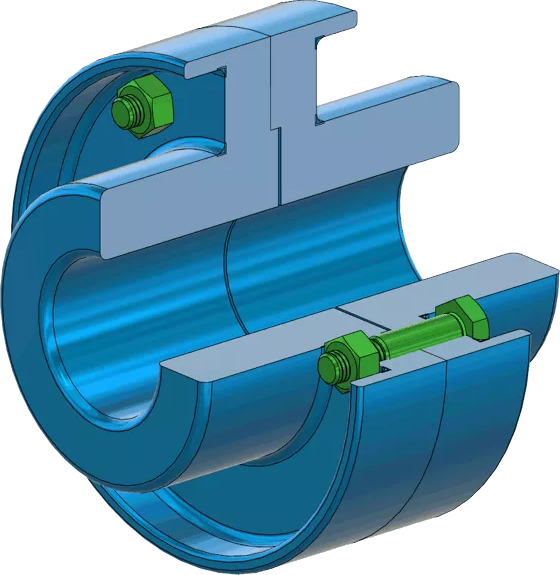
\includegraphics[width=0.68cm,height=0.6cm,keepaspectratio]{graphics/scheibenkupplung.png} & Scheiben- & \MKlvl{4}{hoch--\newline sehr~hoch} & \MKlvl{1}{klein--mittel} & \MKlvl{0}{keine} & \MKlvl{0}{keine} & \MKlvl{0}{keine} \\
  \hline
  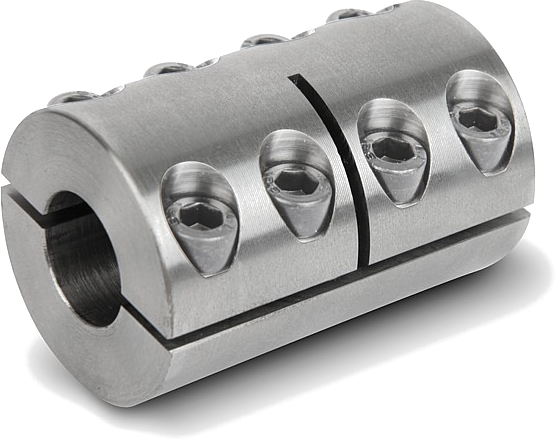
\includegraphics[width=0.68cm,height=0.6cm,keepaspectratio]{graphics/schalenkupplung.png} & Schalen- & \MKlvl{2}{klein--hoch} & \MKlvl{1}{klein--mittel} & \MKlvl{0}{keine} & \MKlvl{0}{keine} & \MKlvl{0}{keine} \\
  \hline
  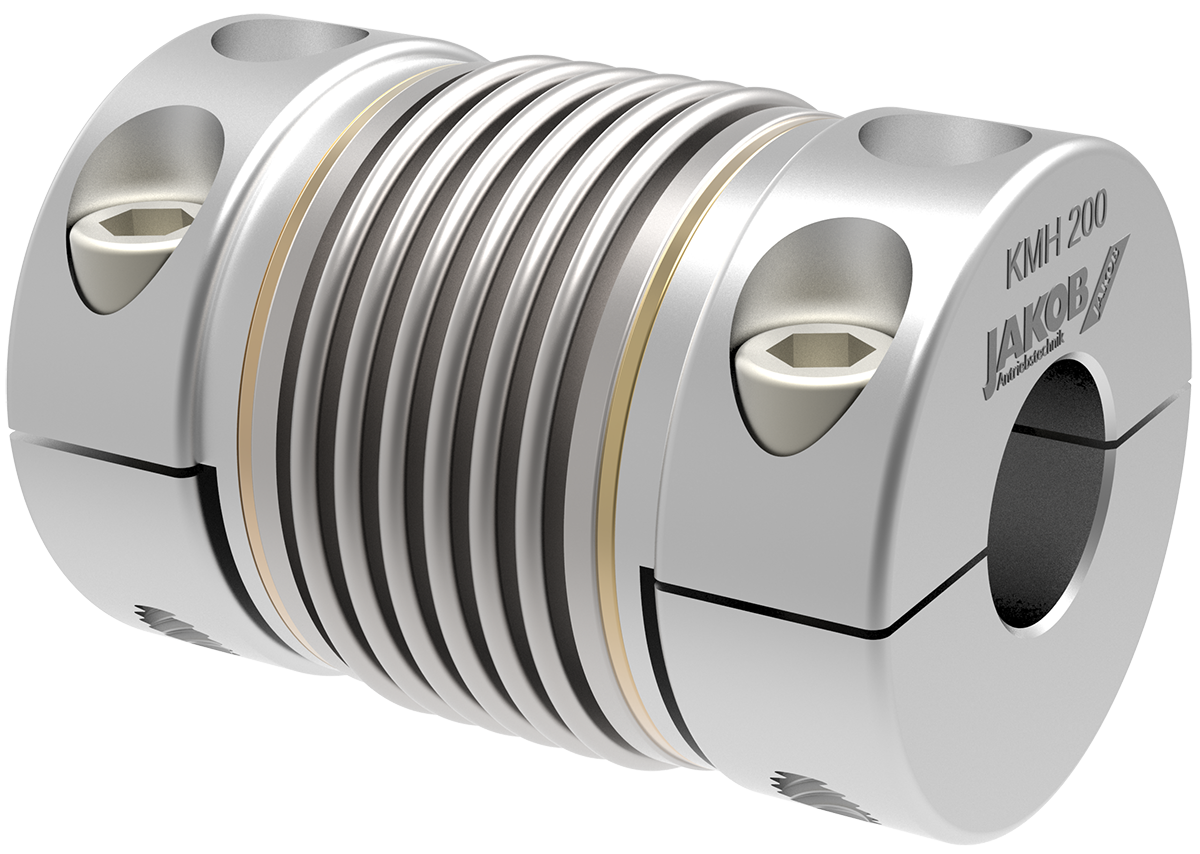
\includegraphics[width=0.68cm,height=0.6cm,keepaspectratio]{graphics/metallbalgkupplung.png} & Metall\-balg- & \MKlvl{3}{mittel--hoch} & \MKlvl{3}{mittel--hoch} & \MKlvl{3}{gut} & \MKlvl{3}{gut} & \MKlvl{4}{sehr gut} \\
  \hline
  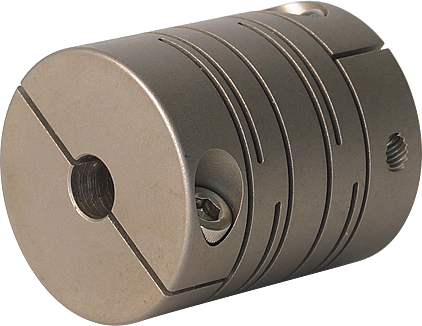
\includegraphics[width=0.68cm,height=0.6cm,keepaspectratio]{graphics/federstegkupplung.png} & Feder\-steg- & \MKlvl{1}{klein--mittel} & \MKlvl{3}{mittel--hoch} & \MKlvl{1}{kaum} & \MKlvl{3}{gut} & \MKlvl{3}{gut} \\
  \hline
  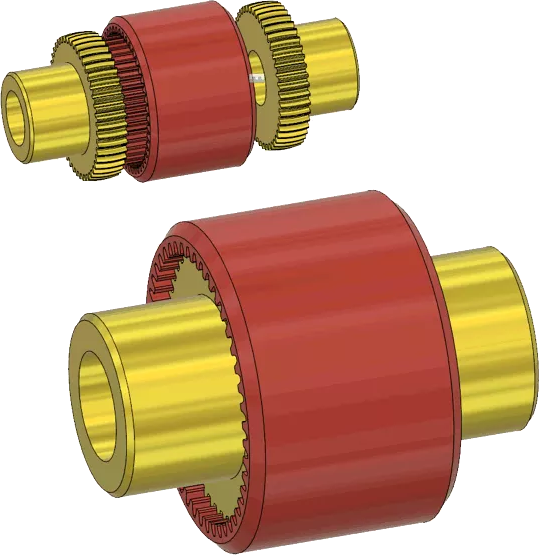
\includegraphics[width=0.68cm,height=0.6cm,keepaspectratio]{graphics/bogenzahnkupplung.png} & Bogen\-zahn- & \MKlvl{4}{hoch--\newline sehr~hoch} & \MKlvl{3}{mittel--hoch} & \MKlvl{3}{gut} & \MKlvl{4}{sehr gut} & \MKlvl{3}{gut} \\
  \hline
  \end{ZSFtablePlain}%
  \arrayrulecolor{black}}%
}

\newcommand{\ZSFKupplungenDrehelastischTabelle}{%
  {\setlength{\tabcolsep}{0.8pt}%
  \arrayrulecolor{black!35}%
  \begin{ZSFtablePlain}[\ZSFfontRel{-3bp}{0.3bp}]{|>{\columncolor{black!8}}Z{0.9}|>{\columncolor{black!8}}Z{1.42}|Z{0.98}|Z{0.95}|Z{0.9}|Z{0.9}|Z{0.95}|}
  \hline
  \ZSFheaderRow \ZSFhead{} & \ZSFhead{Kupplung} & \ZSFhead{Drehmom.} & \ZSFhead{Drehz.} & \multicolumn{3}{c|}{\ZSFhead{Versatz-Ausgleich}} \\
  \ZSFheaderRow \ZSFhead{} & \ZSFhead{} & \ZSFhead{} & \ZSFhead{} & \ZSFhead{axial} & \ZSFhead{radial} & \ZSFhead{winklig} \\
  \noalign{\global\arrayrulewidth=1.1pt}\hline\noalign{\global\arrayrulewidth=0.4pt}%
  \multicolumn{7}{|l|}{\cellcolor{white}\MKrfIcon{icon_drehelastisch}\ \textbf{Drehelastisch}{\color{black!60}: dämpft Stösse, nicht winkelsynchron}} \\
  \noalign{\global\arrayrulewidth=1.1pt}\hline\noalign{\global\arrayrulewidth=0.4pt}%
  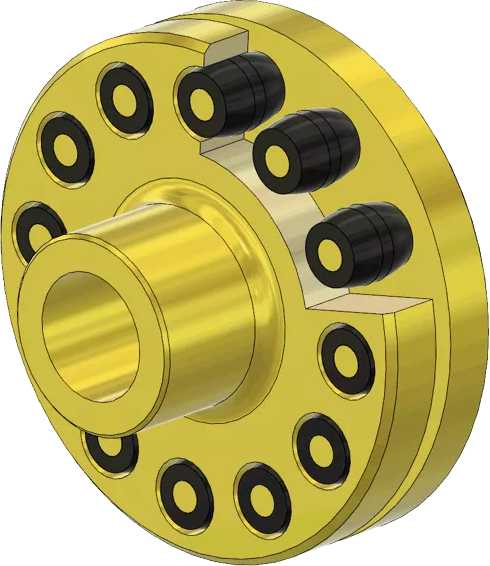
\includegraphics[width=0.68cm,height=0.6cm,keepaspectratio]{graphics/bolzenkupplung.png} & Bolzen- & \MKlvl{4}{hoch--\newline sehr~hoch} & \MKlvl{1}{klein--mittel} & \MKlvl{3}{gut} & \MKlvl{1}{kaum} & \MKlvl{3}{gut} \\
  \hline
  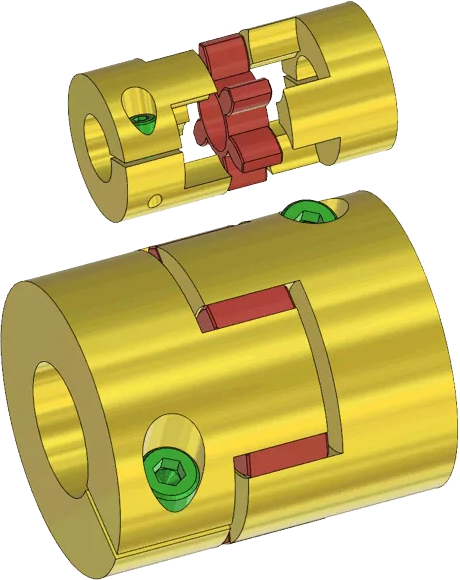
\includegraphics[width=0.68cm,height=0.6cm,keepaspectratio]{graphics/klauenkupplung.png} & Klauen- & \MKlvl{1}{klein--mittel} & \MKlvl{3}{mittel--hoch} & \MKlvl{3}{gut} & \MKlvl{1}{kaum} & \MKlvl{3}{gut} \\
  \hline
  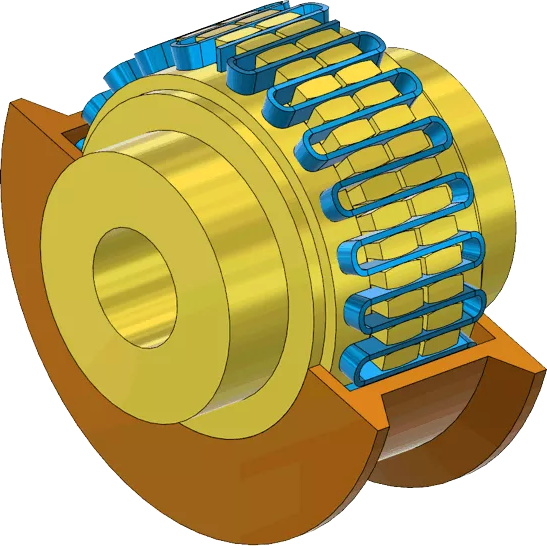
\includegraphics[width=0.68cm,height=0.6cm,keepaspectratio]{graphics/schlangenfederkupplung.png} & Schlangen\-feder- & \MKlvl{3}{mittel--hoch} & \MKlvl{1}{klein--mittel} & \MKlvl{3}{gut} & \MKlvl{3}{gut} & \MKlvl{3}{gut} \\
  \hline
  \end{ZSFtablePlain}%
  \arrayrulecolor{black}}%
}

% ============================================================
% 30_layout_spacing.tex — Layout-Grundlagen, Spacing-Skala, Box-Bindungen
% ============================================================

% MaschKo-Verdichtung: kompakteres parskip (6-Seiten-Budget, bildlastige ZSF)
\setlength{\parskip}{0.5pt plus 0.8pt minus 0.2pt}
% MaschKo-Verdichtung: engere Zeilenabstände (Inspiration nutzte 6.75pt/6pt;
% 0.86 für das 6-Seiten-Ziel — immer noch über der Vorlage (6.75/6 = 0.83)
\linespread{0.74} % 6-Seiten-Ziel: baselineskip ~6.0pt wie die Inspirationsfassung
\setlength{\parindent}{0pt}

\widowpenalty=10000
\clubpenalty=10000
\brokenpenalty=4000
\predisplaypenalty=10000

\raggedcolumns
\newcounter{zsfFirstChap}\setcounter{zsfFirstChap}{1}

% ------------------------------------------------------------
% SPACING-SKALA (4 Stufen) — die einzige Quelle für Abstände
% ------------------------------------------------------------
% MaschKo-Verdichtung: Skala enger als Template-Default (4/7/10)
\newlength{\ZSFspaceXXS}\setlength{\ZSFspaceXXS}{0.5pt} % MaschKo: Mikro-Stufe für Display-Skips (6-Seiten-Ziel)
\newlength{\ZSFspaceXS}\setlength{\ZSFspaceXS}{1pt}
\newlength{\ZSFspaceS} \setlength{\ZSFspaceS}{2pt}
\newlength{\ZSFspaceM} \setlength{\ZSFspaceM}{4pt}
\newlength{\ZSFspaceL} \setlength{\ZSFspaceL}{6pt}

% Outer (Text-Box-Bindung) und Sep (Trennlinien)
\newlength{\ZSFspaceOuter}\setlength{\ZSFspaceOuter}{2pt} % MaschKo-Verdichtung: 4 -> 2 (6-Seiten-Ziel)
\newlength{\ZSFspaceSep}  \setlength{\ZSFspaceSep}{1pt} % MaschKo-Verdichtung: 3 -> 1.5 -> 1 (Trennstriche frassen ~8pt pro \formulasep)

% Corner-Radius-Tokens: runder Grundlook, aber zentral steuerbar.
\newlength{\ZSFcornerBox}   \setlength{\ZSFcornerBox}{0.6mm}
\newlength{\ZSFcornerInline}\setlength{\ZSFcornerInline}{1mm}

% ------------------------------------------------------------
% Spalten-Layout
% ------------------------------------------------------------
\setlength{\columnsep}{4pt} % MaschKo-Verdichtung: L (6pt) -> 4pt (6-Seiten-Ziel)
\setlength{\multicolsep}{\ZSFspaceS}
\setlength{\emergencystretch}{2em}

% ------------------------------------------------------------
% Schwellwerte und Titelbalken-Hilfsgrössen
% ------------------------------------------------------------
\newlength{\ZSFbreakThreshold}\setlength{\ZSFbreakThreshold}{0pt} % Schwellwert minimiert/deaktiviert: verhindert vorzeitige Spaltenumbrüche bei geringem Restplatz
\newlength{\ZSFbreakThresholdChapter}\setlength{\ZSFbreakThresholdChapter}{3\baselineskip} % Mindesthöhe für ChapterBar (verhindert Bars am Spaltenende); MaschKo: 3 statt 10 (Platzbudget; Boxen sind breakable, Bar+erste Teilbox brauchen weniger Reserve)
\newlength{\ZSFpostChapterNudge}\setlength{\ZSFpostChapterNudge}{0pt}
\newlength{\ZSFtitleBarHeight}\setlength{\ZSFtitleBarHeight}{5.8pt} % MaschKo: 9.2 -> 7 -> 5.8 (6-Seiten-Ziel; Strut der Titelschrift bestimmt die effektive Höhe)
\newlength{\ZSFsubsectionBarBeforeSkip}\setlength{\ZSFsubsectionBarBeforeSkip}{4pt} % MaschKo: mehr Luft vor echten Unterthemen, bleibt im 6-Seiten-Budget
\newlength{\ZSFsubsubsectionBarBeforeSkip}\setlength{\ZSFsubsubsectionBarBeforeSkip}{\ZSFspaceXXS} % dritte Ebene: so kompakt wie bisherige Stern-Zwischentitel
\newlength{\ZSFsubsectionAfterChapterGap}\setlength{\ZSFsubsectionAfterChapterGap}{0pt} % Kapitelbalken + erster Abschnitt ohne Zwischenlücke
\newlength{\ZSFsubsectionAfterGap}\setlength{\ZSFsubsectionAfterGap}{\ZSFspaceXS}
\newlength{\ZSFchapterBarAfterSkip}\setlength{\ZSFchapterBarAfterSkip}{1pt} % MaschKo-Verdichtung: 2 -> 1 (6-Seiten-Ziel)

% Maximale Höhe für Bilder in figboxen (verhindert überhohe Aspect-Ratios).
\newlength{\ZSFfigMaxHeight}\setlength{\ZSFfigMaxHeight}{2.6cm}
% Globaler Skalierungsfaktor für \ZSFfig-Bilder (Seitenbudget-Hebel).
% Getestet (2026-07): 0.93 reduziert die Seitenzahl NICHT (Packverlust
% dominiert) — deshalb 1.0 = exakte Vorlagen-Verhältnisse. Werte bis 0.90
% liegen innerhalb der 10%-Toleranz, falls später nötig.
\newcommand{\ZSFfigScale}{1.0}

% Tokens für statementbox / procedure
\newlength{\ZSFstatementBarWidth}\setlength{\ZSFstatementBarWidth}{2pt}
\newlength{\ZSFstatementLeftPad} \setlength{\ZSFstatementLeftPad}{\ZSFspaceM}
\newlength{\ZSFprocStepGap}      \setlength{\ZSFprocStepGap}{\ZSFspaceXS}
\newlength{\ZSFprocItemSep}      \setlength{\ZSFprocItemSep}{\ZSFspaceXS}

% Padding für cellspace (siehe styles/20_tables.tex Konvention)
\newlength{\ZSFtextMinPad}\setlength{\ZSFtextMinPad}{\ZSFspaceXS}

% ------------------------------------------------------------
% Code-Längen — nur für die optionalen Code-Module benötigt
% (styles/65_code_style.tex + 67_code_comments.tex). Schadlos
% wenn die Module in preamble.tex deaktiviert sind.
% MaxWidth:   max. Breite des rechts-stehenden Kommentars
% Threshold:  Schwelle für Auto-Overflow (Code+Kommentar > Threshold -> oben)
% Default-Register sind immutabel und dienen \ResetCodeCommentThreshold
% als Anker; \SetCodeCommentThreshold modifiziert nur die "lebenden" Register.
% ------------------------------------------------------------
\newlength{\ZSFcodeMiniSkip}  \setlength{\ZSFcodeMiniSkip}{1mm}
\newlength{\ZSFcodeFrameRule} \setlength{\ZSFcodeFrameRule}{0.4pt}
\newlength{\ZSFcodeXMargin}   \setlength{\ZSFcodeXMargin}{8pt}
\newlength{\ZSFcodeCommentMaxWidthDefault}
  \setlength{\ZSFcodeCommentMaxWidthDefault}{.25\columnwidth}
\newlength{\ZSFcodeCommentThresholdDefault}
  \setlength{\ZSFcodeCommentThresholdDefault}{\maxdimen}
\newlength{\ZSFcodeCommentMaxWidth} \setlength{\ZSFcodeCommentMaxWidth}{\ZSFcodeCommentMaxWidthDefault}
\newlength{\ZSFcodeCommentThreshold}\setlength{\ZSFcodeCommentThreshold}{\ZSFcodeCommentThresholdDefault}
\newlength{\ZSFcodeCommentGap}      \setlength{\ZSFcodeCommentGap}{\ZSFspaceM}

% ============================================================
% TEXT-BOX-BINDUNGEN
% Koppeln Fliesstext direkt an Boxen — verhindert visuellen Bruch.
% ============================================================

% Robustes Skip-/Penalty-Aufrollen (vmode-/hmode-aware)
\newcommand{\ZSFRobustUnskip}{%
  \ifvmode
    \ifdim\lastskip>0pt\relax\vskip-\lastskip\fi
    \ifnum\lastpenalty=0\else\unpenalty\fi
    \ifdim\lastskip>0pt\relax\vskip-\lastskip\fi
  \else
    \ifdim\lastskip>0pt\relax\unskip\fi
    \ifnum\lastpenalty=0\else\unpenalty\fi
    \ifdim\lastskip>0pt\relax\unskip\fi
  \fi
}

% Text der zur Box DARUNTER gehört (Einleitung)
\newcommand{\textVorBox}[1]{%
  \par
  \addvspace{\ZSFspaceOuter}%
  \begingroup
  \setlength{\parskip}{0pt}%
  {\small\color{TextVorBoxColor} \noindent #1\par}%
  \endgroup
  \nopagebreak
  \vspace{\ZSFspaceXS}%
  \vspace{-\ZSFspaceS}%
  \nopagebreak
}

% Text der zur Box DARÜBER gehört (Ergänzung/Folgerung)
\newcommand{\textNachBox}[1]{%
  \par
  \ZSFRobustUnskip
  \vspace{\ZSFspaceXS}%
  \begingroup
  \setlength{\parskip}{0pt}%
  \nopagebreak
  {\small\color{TextNachBoxColor} \noindent #1\par}%
  \endgroup
  \addvspace{\ZSFspaceOuter}%
}

% Titel/Text vor einer Formel (innerhalb der formulabox)
\newcommand{\textVorFormel}[1]{%
  \par
  \begingroup
  \setlength{\parskip}{0pt}%
  \noindent\raggedright\textcolor{black!60}{\textbf{#1}}\par
  \endgroup
  \vspace{\ZSFspaceXS}%
  \centering
}

% Erklaerungstext nach einer Formel (innerhalb der formulabox)
\newcommand{\textNachFormel}[1]{%
  \par
  \vspace{\ZSFspaceXS}%
  \begingroup
  \setlength{\parskip}{0pt}%
  \noindent\raggedright\textcolor{black!60}{\small #1}\par
  \endgroup
  \centering
}

% ------------------------------------------------------------
% Semantische Gap-Helfer für Kapitel (sparsam einsetzen)
% ------------------------------------------------------------
\newcommand{\ZSFSectionGap}{\vspace{\ZSFspaceL}}
\newcommand{\ZSFgapXS}{\vspace{\ZSFspaceXS}}
\newcommand{\ZSFgapS}{\vspace{\ZSFspaceS}}
\newcommand{\ZSFgapM}{\vspace{\ZSFspaceM}}
\newcommand{\ZSFgapL}{\vspace{\ZSFspaceL}}
\newcommand{\ZSFmanualColumnBreak}{\columnbreak}
\newcommand{\ZSFtabColGap}{\hspace{1.5em}}

\input{styles/40_colors_structure}
% ============================================================
% 42_gear_variable_colors.tex -- Zahnrad-Variablenfarben
% ============================================================
%
% Zweck fuer die Pruefung:
% Farben dienen als Lookup-Hilfe beim Zusammensetzen von Formeln.
% Die Hauptfarbe macht Variablenfamilien und wichtige Varianten wie d_a,
% d_b, m, z oder epsilon_* an ihren Berechnungsstellen schnell auffindbar.
% Unterschiedliche kleine Zusaetze schuetzen vor Verwechslungen. Objektindizes
% wie 1, 2, 3 und s koennen eine zusaetzliche Indexfarbe tragen, damit
% gleichartige Groessen dem richtigen Zahnrad bzw. Steg zugeordnet werden.
% Farben muessen nicht projektweit eindeutig sein; entscheidend ist die
% praktische Unterscheidbarkeit im Formelblock und entlang des Lookup-Pfads.
% Neue Zahnradvariablen sollen hier als eigene Makros abgebildet werden,
% wenn sie sonst mit aehnlich geschriebenen Groessen verwechselt werden.

\definecolor{GearVarGeomColor}{HTML}{00796B}
\definecolor{GearVarToothColor}{HTML}{2E7D32}
\definecolor{GearVarAngleColor}{HTML}{6D28D9}
\definecolor{GearVarMotionColor}{HTML}{334155}
\definecolor{GearVarLoadColor}{HTML}{B42318}
\definecolor{GearVarMomentColor}{HTML}{5B21B6}
\definecolor{GearVarPowerColor}{HTML}{006B5B}
\definecolor{GearVarSpeedColor}{HTML}{0F5E9C}
\definecolor{GearVarToothThicknessColor}{HTML}{D0006F}
\definecolor{GearVarToothSpaceColor}{HTML}{0284C7}
\definecolor{GearVarStrengthColor}{HTML}{4C1D95}
\definecolor{GearObjOneColor}{HTML}{E11D48}
\definecolor{GearObjTwoColor}{HTML}{2563EB}
\definecolor{GearObjThreeColor}{HTML}{D97706}
\definecolor{GearObjFourColor}{HTML}{7C3AED}
\definecolor{GearObjCarrierColor}{HTML}{059669}
\definecolor{GearRoleSlidingColor}{HTML}{D0006F}
\definecolor{GearRoleRollingColor}{HTML}{2E7D32}
\definecolor{GearRoleTangentialColor}{HTML}{4C1D95}
\definecolor{GearRoleRadialColor}{HTML}{0F766E}
\definecolor{GearRoleAxialColor}{HTML}{D0006F}
\definecolor{GearRoleNormalColor}{HTML}{2563EB}
\definecolor{GearRoleMeanColor}{HTML}{B45309}
\definecolor{GearRoleOperatingColor}{HTML}{D0006F}
\definecolor{GearRoleTransverseColor}{HTML}{EA580C}
\definecolor{GearRoleAlphaColor}{HTML}{2563EB}
\definecolor{GearRoleBetaColor}{HTML}{EA580C}
\definecolor{GearRoleGammaColor}{HTML}{059669}
\definecolor{GearRoleDerivedColor}{HTML}{B45309}
\definecolor{GearRoleEquivalentColor}{HTML}{059669}
\definecolor{GearVarCenterColor}{HTML}{0057B8}
\definecolor{GearVarDiaPitchColor}{HTML}{0F766E}
\definecolor{GearVarDiaHeadColor}{HTML}{D0006F}
\definecolor{GearVarDiaRootColor}{HTML}{EA580C}
\definecolor{GearVarDiaBaseColor}{HTML}{7C3AED}
\definecolor{GearVarHeightHeadColor}{HTML}{0284C7}
\definecolor{GearVarHeightRootColor}{HTML}{C2410C}
\definecolor{GearVarModuleColor}{HTML}{2E7D32}
\definecolor{GearVarToothCountColor}{HTML}{B45309}
\definecolor{GearVarPitchColor}{HTML}{A21CAF}
\definecolor{GearVarWidthColor}{HTML}{0F766E}
\definecolor{GearVarJumpColor}{HTML}{0F5E9C}
\definecolor{GearVarShiftColor}{HTML}{D0006F}
\definecolor{GearVarContactColor}{HTML}{4D7C0F}
\definecolor{GearVarOverlapColor}{HTML}{DC2626}

\newcommand{\ZSFgearGeom}[1]{\ZSFVariableColor{GearVarGeomColor}{#1}}
\newcommand{\ZSFgearTooth}[1]{\ZSFVariableColor{GearVarToothColor}{#1}}
\newcommand{\ZSFgearAngle}[1]{\ZSFVariableColor{GearVarAngleColor}{#1}}
\newcommand{\ZSFgearMotion}[1]{\ZSFVariableColor{GearVarMotionColor}{#1}}
\newcommand{\ZSFgearLoad}[1]{\ZSFVariableColor{GearVarLoadColor}{#1}}
\newcommand{\ZSFgearMoment}[1]{\ZSFVariableColor{GearVarMomentColor}{#1}}
\newcommand{\ZSFgearPower}[1]{\ZSFVariableColor{GearVarPowerColor}{#1}}
\newcommand{\ZSFgearSpeed}[1]{\ZSFVariableColor{GearVarSpeedColor}{#1}}
\newcommand{\ZSFgearToothThickness}[1]{\ZSFVariableColor{GearVarToothThicknessColor}{#1}}
\newcommand{\ZSFgearToothSpace}[1]{\ZSFVariableColor{GearVarToothSpaceColor}{#1}}
\newcommand{\ZSFgearStrength}[1]{\ZSFVariableColor{GearVarStrengthColor}{#1}}
\newcommand{\ZSFgearOne}[1]{\ZSFVariableColor{GearObjOneColor}{#1}}
\newcommand{\ZSFgearTwo}[1]{\ZSFVariableColor{GearObjTwoColor}{#1}}
\newcommand{\ZSFgearThree}[1]{\ZSFVariableColor{GearObjThreeColor}{#1}}
\newcommand{\ZSFgearFour}[1]{\ZSFVariableColor{GearObjFourColor}{#1}}
\newcommand{\ZSFgearCarrier}[1]{\ZSFVariableColor{GearObjCarrierColor}{#1}}
\newcommand{\ZSFgearRoleSliding}[1]{\ZSFVariableColor{GearRoleSlidingColor}{#1}}
\newcommand{\ZSFgearRoleRolling}[1]{\ZSFVariableColor{GearRoleRollingColor}{#1}}
\newcommand{\ZSFgearRoleTangential}[1]{\ZSFVariableColor{GearRoleTangentialColor}{#1}}
\newcommand{\ZSFgearRoleRadial}[1]{\ZSFVariableColor{GearRoleRadialColor}{#1}}
\newcommand{\ZSFgearRoleAxial}[1]{\ZSFVariableColor{GearRoleAxialColor}{#1}}
\newcommand{\ZSFgearRoleNormal}[1]{\ZSFVariableColor{GearRoleNormalColor}{#1}}
\newcommand{\ZSFgearRoleMean}[1]{\ZSFVariableColor{GearRoleMeanColor}{#1}}
\newcommand{\ZSFgearRoleOperating}[1]{\ZSFVariableColor{GearRoleOperatingColor}{#1}}
\newcommand{\ZSFgearRoleTransverse}[1]{\ZSFVariableColor{GearRoleTransverseColor}{#1}}
\newcommand{\ZSFgearRoleAlpha}[1]{\ZSFVariableColor{GearRoleAlphaColor}{#1}}
\newcommand{\ZSFgearRoleBeta}[1]{\ZSFVariableColor{GearRoleBetaColor}{#1}}
\newcommand{\ZSFgearRoleGamma}[1]{\ZSFVariableColor{GearRoleGammaColor}{#1}}
\newcommand{\ZSFgearRoleDerived}[1]{\ZSFVariableColor{GearRoleDerivedColor}{#1}}
\newcommand{\ZSFgearRoleEquivalent}[1]{\ZSFVariableColor{GearRoleEquivalentColor}{#1}}

\newcommand{\ZSFgearIndexOne}[1]{\ZSFVariableColor{GearObjOneColor}{#1}}
\newcommand{\ZSFgearIndexTwo}[1]{\ZSFVariableColor{GearObjTwoColor}{#1}}
\newcommand{\ZSFgearIndexThree}[1]{\ZSFVariableColor{GearObjThreeColor}{#1}}
\newcommand{\ZSFgearIndexFour}[1]{\ZSFVariableColor{GearObjFourColor}{#1}}
\newcommand{\ZSFgearIndexCarrier}[1]{\ZSFVariableColor{GearObjCarrierColor}{#1}}

\newcommand{\ZSFgearCenter}[1]{\ZSFVariableColor{GearVarCenterColor}{#1}}
\newcommand{\ZSFgearDiaPitch}[1]{\ZSFVariableColor{GearVarDiaPitchColor}{#1}}
\newcommand{\ZSFgearDiaHead}[1]{\ZSFVariableColor{GearVarDiaHeadColor}{#1}}
\newcommand{\ZSFgearDiaRoot}[1]{\ZSFVariableColor{GearVarDiaRootColor}{#1}}
\newcommand{\ZSFgearDiaBase}[1]{\ZSFVariableColor{GearVarDiaBaseColor}{#1}}
\newcommand{\ZSFgearHeightHead}[1]{\ZSFVariableColor{GearVarHeightHeadColor}{#1}}
\newcommand{\ZSFgearHeightRoot}[1]{\ZSFVariableColor{GearVarHeightRootColor}{#1}}
\newcommand{\ZSFgearModule}[1]{\ZSFVariableColor{GearVarModuleColor}{#1}}
\newcommand{\ZSFgearToothCount}[1]{\ZSFVariableColor{GearVarToothCountColor}{#1}}
\newcommand{\ZSFgearPitch}[1]{\ZSFVariableColor{GearVarPitchColor}{#1}}
\newcommand{\ZSFgearWidth}[1]{\ZSFVariableColor{GearVarWidthColor}{#1}}
\newcommand{\ZSFgearJump}[1]{\ZSFVariableColor{GearVarJumpColor}{#1}}
\newcommand{\ZSFgearShift}[1]{\ZSFVariableColor{GearVarShiftColor}{#1}}
\newcommand{\ZSFgearContact}[1]{\ZSFVariableColor{GearVarContactColor}{#1}}
\newcommand{\ZSFgearOverlap}[1]{\ZSFVariableColor{GearVarOverlapColor}{#1}}

\newcommand{\ZSFgearA}{\ZSFgearCenter{a}}
\newcommand{\ZSFgearAd}{\ZSFgearCenter{a}_{\ZSFgearRoleDerived{d}}}
\newcommand{\ZSFgearD}{\ZSFgearDiaPitch{d}}
\newcommand{\ZSFgearDOne}{\ZSFgearDiaPitch{d_{\ZSFgearIndexOne{1}}}}
\newcommand{\ZSFgearDTwo}{\ZSFgearDiaPitch{d_{\ZSFgearIndexTwo{2}}}}
\newcommand{\ZSFgearDThree}{\ZSFgearDiaPitch{d_{\ZSFgearIndexThree{3}}}}
\newcommand{\ZSFgearDp}{\ZSFgearDiaPitch{d_p}}
\newcommand{\ZSFgearDsh}{\ZSFgearDiaPitch{d_{sh}}}
\newcommand{\ZSFgearDmOne}{\ZSFgearDiaPitch{d_{m\ZSFgearIndexOne{1}}}}
\newcommand{\ZSFgearDmTwo}{\ZSFgearDiaPitch{d_{m\ZSFgearIndexTwo{2}}}}
\newcommand{\ZSFgearDeOne}{\ZSFgearDiaPitch{d_{e\ZSFgearIndexOne{1}}}}
\newcommand{\ZSFgearDeTwo}{\ZSFgearDiaPitch{d_{e\ZSFgearIndexTwo{2}}}}
\newcommand{\ZSFgearDa}{\ZSFgearDiaHead{d_a}}
\newcommand{\ZSFgearDaOne}{\ZSFgearDiaHead{d_{a\ZSFgearIndexOne{1}}}}
\newcommand{\ZSFgearDaTwo}{\ZSFgearDiaHead{d_{a\ZSFgearIndexTwo{2}}}}
\newcommand{\ZSFgearDf}{\ZSFgearDiaRoot{d_f}}
\newcommand{\ZSFgearDb}{\ZSFgearDiaBase{d_b}}
\newcommand{\ZSFgearDbOne}{\ZSFgearDiaBase{d_{b\ZSFgearIndexOne{1}}}}
\newcommand{\ZSFgearDbTwo}{\ZSFgearDiaBase{d_{b\ZSFgearIndexTwo{2}}}}
\newcommand{\ZSFgearHa}{\ZSFgearHeightHead{h_a}}
\newcommand{\ZSFgearHf}{\ZSFgearHeightRoot{h_f}}
\newcommand{\ZSFgearH}{\ZSFgearGeom{h}}
\newcommand{\ZSFgearM}{\ZSFgearModule{m}}
\newcommand{\ZSFgearMOne}{\ZSFgearModule{m_{\ZSFgearIndexOne{1}}}}
\newcommand{\ZSFgearMTwo}{\ZSFgearModule{m_{\ZSFgearIndexTwo{2}}}}
\newcommand{\ZSFgearMn}{\ZSFgearModule{m}_{\ZSFgearRoleNormal{n}}}
\newcommand{\ZSFgearMnTriplePrime}{\ZSFgearModule{m}_{\ZSFgearRoleNormal{n}}^{\prime\prime\prime}}
\newcommand{\ZSFgearMt}{\ZSFgearModule{m}_{\ZSFgearRoleTransverse{t}}}
\newcommand{\ZSFgearZ}{\ZSFgearToothCount{z}}
\newcommand{\ZSFgearZOne}{\ZSFgearToothCount{z_{\ZSFgearIndexOne{1}}}}
\newcommand{\ZSFgearZTwo}{\ZSFgearToothCount{z_{\ZSFgearIndexTwo{2}}}}
\newcommand{\ZSFgearZThree}{\ZSFgearToothCount{z_{\ZSFgearIndexThree{3}}}}
\newcommand{\ZSFgearZFour}{\ZSFgearToothCount{z_{\ZSFgearIndexFour{4}}}}
\newcommand{\ZSFgearZg}{\ZSFgearToothCount{z_g}}
\newcommand{\ZSFgearZgPrime}{\ZSFgearToothCount{z_g'}}
\newcommand{\ZSFgearZgtPrime}{\ZSFgearToothCount{z_{gt}'}}
\newcommand{\ZSFgearZGross}{\ZSFgearToothCount{z_{\text{Grossrad}}}}
\newcommand{\ZSFgearZKlein}{\ZSFgearToothCount{z_{\text{Kleinrad}}}}
\newcommand{\ZSFgearP}{\ZSFgearPitch{p}}
\newcommand{\ZSFgearPe}{\ZSFgearPitch{p}_{\ZSFgearRoleDerived{e}}}
\newcommand{\ZSFgearPt}{\ZSFgearPitch{p}_{\ZSFgearRoleTransverse{t}}}
\newcommand{\ZSFgearU}{\ZSFgearGeom{U}}
\newcommand{\ZSFgearUJump}{\ZSFgearJump{U}}
\newcommand{\ZSFgearB}{\ZSFgearWidth{b}}
\newcommand{\ZSFgearBOne}{\ZSFgearWidth{b_{\ZSFgearIndexOne{1}}}}
\newcommand{\ZSFgearC}{\ZSFgearGeom{c}}
\newcommand{\ZSFgearGa}{\ZSFgearContact{g_a}}
\newcommand{\ZSFgearGalpha}{\ZSFgearContact{g}_{\ZSFgearRoleAlpha{\alpha}}}
\newcommand{\ZSFgearEpsAlpha}{\ZSFgearOverlap{\varepsilon}_{\ZSFgearRoleAlpha{\alpha}}}
\newcommand{\ZSFgearEpsAlphaBrace}{\ZSFgearOverlap{\varepsilon}_{\ZSFgearRoleAlpha{\alpha}}}
\newcommand{\ZSFgearEpsBeta}{\ZSFgearOverlap{\varepsilon}_{\ZSFgearRoleBeta{\beta}}}
\newcommand{\ZSFgearEpsGamma}{\ZSFgearOverlap{\varepsilon}_{\ZSFgearRoleGamma{\gamma}}}
\newcommand{\ZSFgearEpsAll}{\ZSFgearOverlap{\varepsilon}_{\ZSFgearRoleAlpha{\alpha}/\ZSFgearRoleBeta{\beta}/\ZSFgearRoleGamma{\gamma}}}
\newcommand{\ZSFgearX}{\ZSFgearShift{x}}
\newcommand{\ZSFgearXOne}{\ZSFgearShift{x_{\ZSFgearIndexOne{1}}}}
\newcommand{\ZSFgearXTwo}{\ZSFgearShift{x_{\ZSFgearIndexTwo{2}}}}
\newcommand{\ZSFgearSOne}{\ZSFgearShift{s_{\ZSFgearIndexOne{1}}}}
\newcommand{\ZSFgearSTwo}{\ZSFgearShift{s_{\ZSFgearIndexTwo{2}}}}
\newcommand{\ZSFgearV}{\ZSFgearShift{V}}
\newcommand{\ZSFgearVplus}{\ZSFgearShift{V_{plus}}}
\newcommand{\ZSFgearVminus}{\ZSFgearShift{V_{minus}}}
\newcommand{\ZSFgearPsi}{\ZSFgearWidth{\psi}}
\newcommand{\ZSFgearPsid}{\ZSFgearWidth{\psi_d}}
\newcommand{\ZSFgearEta}{\ZSFgearMotion{\eta}}
\newcommand{\ZSFgearAlpha}{\ZSFgearAngle{\alpha}}
\newcommand{\ZSFgearAlphaW}{\ZSFgearAngle{\alpha}_{\ZSFgearRoleOperating{w}}}
\newcommand{\ZSFgearAlphaN}{\ZSFgearAngle{\alpha}_{\ZSFgearRoleNormal{n}}}
\newcommand{\ZSFgearAlphaT}{\ZSFgearAngle{\alpha}_{\ZSFgearRoleTransverse{t}}}
\newcommand{\ZSFgearAlphaWT}{\ZSFgearAngle{\alpha}_{\ZSFgearRoleOperating{w}\ZSFgearRoleTransverse{t}}}
\newcommand{\ZSFgearBeta}{\ZSFgearAngle{\beta}}
\newcommand{\ZSFgearSigmaAngle}{\ZSFgearAngle{\Sigma}}
\newcommand{\ZSFgearDeltaOne}{\ZSFgearAngle{\delta}_{\ZSFgearIndexOne{1}}}
\newcommand{\ZSFgearDeltaTwo}{\ZSFgearAngle{\delta}_{\ZSFgearIndexTwo{2}}}
\newcommand{\ZSFgearF}{\ZSFgearLoad{F}}
\newcommand{\ZSFgearFOne}{\ZSFgearLoad{F}_{\ZSFgearIndexOne{1}}}
\newcommand{\ZSFgearFt}{\ZSFgearLoad{F}_{\ZSFgearRoleTangential{t}}}
\newcommand{\ZSFgearFr}{\ZSFgearLoad{F}_{\ZSFgearRoleRadial{r}}}
\newcommand{\ZSFgearFa}{\ZSFgearLoad{F}_{\ZSFgearRoleAxial{a}}}
\newcommand{\ZSFgearFn}{\ZSFgearLoad{F}_{\ZSFgearRoleNormal{n}}}
\newcommand{\ZSFgearFtOne}{\ZSFgearLoad{F}_{\ZSFgearRoleTangential{t}\ZSFgearIndexOne{1}}}
\newcommand{\ZSFgearFtTwo}{\ZSFgearLoad{F}_{\ZSFgearRoleTangential{t}\ZSFgearIndexTwo{2}}}
\newcommand{\ZSFgearFrOne}{\ZSFgearLoad{F}_{\ZSFgearRoleRadial{r}\ZSFgearIndexOne{1}}}
\newcommand{\ZSFgearFrTwo}{\ZSFgearLoad{F}_{\ZSFgearRoleRadial{r}\ZSFgearIndexTwo{2}}}
\newcommand{\ZSFgearFaOne}{\ZSFgearLoad{F}_{\ZSFgearRoleAxial{a}\ZSFgearIndexOne{1}}}
\newcommand{\ZSFgearFaTwo}{\ZSFgearLoad{F}_{\ZSFgearRoleAxial{a}\ZSFgearIndexTwo{2}}}
\newcommand{\ZSFgearFtnOne}{\ZSFgearLoad{F}_{\ZSFgearRoleTangential{t}\ZSFgearRoleNormal{n}\ZSFgearIndexOne{1}}}
\newcommand{\ZSFgearFmtOne}{\ZSFgearLoad{F}_{\ZSFgearRoleMean{m}\ZSFgearRoleTangential{t}\ZSFgearIndexOne{1}}}
\newcommand{\ZSFgearFmtTwo}{\ZSFgearLoad{F}_{\ZSFgearRoleMean{m}\ZSFgearRoleTangential{t}\ZSFgearIndexTwo{2}}}
\newcommand{\ZSFgearFtTooth}{\ZSFgearLoad{F}_{\ZSFgearRoleTangential{t},\text{\ZSFgearTooth{Zahn}}}}
\newcommand{\ZSFgearDTooth}{\ZSFgearDiaPitch{d}_{\text{\ZSFgearTooth{Zahn}}}}
\newcommand{\ZSFgearTorque}{\ZSFgearMoment{M}}
\newcommand{\ZSFgearTorqueOne}{\ZSFgearMoment{M}_{\ZSFgearIndexOne{1}}}
\newcommand{\ZSFgearTorqueTwo}{\ZSFgearMoment{M}_{\ZSFgearIndexTwo{2}}}
\newcommand{\ZSFgearTorqueAn}{\ZSFgearMoment{M}_{\ZSFgearIndexOne{an}}}
\newcommand{\ZSFgearTorqueAb}{\ZSFgearMoment{M}_{\ZSFgearIndexTwo{ab}}}
\newcommand{\ZSFgearTorqueEqOne}{\ZSFgearMoment{T}_{\ZSFgearIndexOne{1}\ZSFgearRoleEquivalent{eq}}}
\newcommand{\ZSFgearSigmaFlimOne}{\ZSFgearStrength{\sigma}_{\ZSFgearRoleAxial{F}\ZSFgearMotion{lim}\ZSFgearIndexOne{1}}}
\newcommand{\ZSFgearPowerAn}{\ZSFgearPower{P}_{\ZSFgearIndexOne{\text{an}}}}
\newcommand{\ZSFgearPowerAb}{\ZSFgearPower{P}_{\ZSFgearIndexTwo{\text{ab}}}}
\newcommand{\ZSFgearOmegaOne}{\ZSFgearSpeed{\omega}_{\ZSFgearIndexOne{1}}}
\newcommand{\ZSFgearOmegaTwo}{\ZSFgearSpeed{\omega}_{\ZSFgearIndexTwo{2}}}
\newcommand{\ZSFgearNOne}{\ZSFgearSpeed{n}_{\ZSFgearIndexOne{1}}}
\newcommand{\ZSFgearNTwo}{\ZSFgearSpeed{n}_{\ZSFgearIndexTwo{2}}}
\newcommand{\ZSFgearNThree}{\ZSFgearSpeed{n}_{\ZSFgearIndexThree{3}}}
\newcommand{\ZSFgearNCarrier}{\ZSFgearSpeed{n}_{\ZSFgearIndexCarrier{s}}}
\newcommand{\ZSFgearNAn}{\ZSFgearSpeed{n}_{\ZSFgearIndexOne{\text{an}}}}
\newcommand{\ZSFgearNAb}{\ZSFgearSpeed{n}_{\ZSFgearIndexTwo{\text{ab}}}}
\newcommand{\ZSFgearROne}{\ZSFgearDiaPitch{r}_{\ZSFgearIndexOne{1}}}
\newcommand{\ZSFgearRTwo}{\ZSFgearDiaPitch{r}_{\ZSFgearIndexTwo{2}}}
\newcommand{\ZSFgearR}{\ZSFgearDiaPitch{r}}
\newcommand{\ZSFgearSwOne}{\ZSFgearToothThickness{S}_{\ZSFgearMotion{w}\ZSFgearIndexOne{1}}}
\newcommand{\ZSFgearSwTwo}{\ZSFgearToothThickness{S}_{\ZSFgearMotion{w}\ZSFgearIndexTwo{2}}}
\newcommand{\ZSFgearSw}{\ZSFgearToothThickness{s}_{\ZSFgearMotion{w}}}
\newcommand{\ZSFgearEwOne}{\ZSFgearToothSpace{e}_{\ZSFgearMotion{w}\ZSFgearIndexOne{1}}}
\newcommand{\ZSFgearEwTwo}{\ZSFgearToothSpace{e}_{\ZSFgearMotion{w}\ZSFgearIndexTwo{2}}}
\newcommand{\ZSFgearEw}{\ZSFgearToothSpace{e}_{\ZSFgearMotion{w}}}
\newcommand{\ZSFgearS}{\ZSFgearToothThickness{s}}
\newcommand{\ZSFgearSlip}{\ZSFgearMotion{s}}
\newcommand{\ZSFgearVSliding}{\ZSFgearMotion{V}_{\ZSFgearRoleSliding{\text{gleit}}}}
\newcommand{\ZSFgearVRolling}{\ZSFgearMotion{V}_{\ZSFgearRoleRolling{\text{roll}}}}

% ============================================================
% 43_machine_variable_colors.tex -- Maschinenbau-Variablenfarben
% ============================================================
%
% Zweck fuer die Pruefung:
% Farben dienen als Lookup-Hilfe beim Zusammensetzen von Formeln.
% Hauptziel ist das schnelle Wiederfinden von Berechnungs- und Einsatzstellen.
% Das Grundsymbol markiert meist die Groessenfamilie, der Index/Zusatz trennt
% Rolle, Objekt oder Zustand und schuetzt so vor Verwechslungen.
% Dadurch bleiben z. B. F_B, F_BS und F_BT erkennbar verwandt, aber nicht
% verwechselbar.
%
% Regeln fuer Erweiterungen:
% - Kapitel verwenden nur konkrete Makros wie \ZSFscrewFB, keine rohen Farben.
% - Farben duerfen in getrennten, nicht verwechslungsgefaehrdeten Kontexten
%   wiederverwendet werden; Symbol, Index und Kontext bleiben massgebend.
% - Bei zusammengesetzten Variablen Grundsymbol und Subskript getrennt faerben,
%   wenn der Subskript fachlich einen anderen Wert/Rollenanteil markiert.
% - Vor neuen Farben zuerst pruefen, ob im gleichen Formelblock eine
%   Verwechslung mit bestehenden Variablen entstehen wuerde.

\definecolor{MechVarForceColor}{HTML}{991B1B}
\definecolor{MechVarMomentColor}{HTML}{5B21B6}
\definecolor{MechVarStressColor}{HTML}{BE185D}
\definecolor{MechVarShearColor}{HTML}{0E7490}
\definecolor{MechVarDiameterColor}{HTML}{047857}
\definecolor{MechVarDiameterAltColor}{HTML}{0369A1}
\definecolor{MechVarLengthColor}{HTML}{1D4ED8}
\definecolor{MechVarAreaColor}{HTML}{166534}
\definecolor{MechVarAngleColor}{HTML}{7E22CE}
\definecolor{MechVarMaterialColor}{HTML}{3F6212}
\definecolor{MechVarSafetyColor}{HTML}{1F2937}
\definecolor{MechVarStiffnessColor}{HTML}{92400E}
\definecolor{MechVarPressureColor}{HTML}{C2410C}
\definecolor{MechVarDeflectionColor}{HTML}{BE123C}
\definecolor{MechVarFrictionColor}{HTML}{475569}
\definecolor{MechVarFactorColor}{HTML}{9333EA}
\definecolor{MechVarPitchColor}{HTML}{A21CAF}
\definecolor{MechVarWorkColor}{HTML}{065F46}
\definecolor{MechVarPreloadColor}{HTML}{1E40AF}
\definecolor{MechVarOperatingLoadColor}{HTML}{A16207}
\definecolor{MechVarSettlementColor}{HTML}{DB2777}
\definecolor{MechVarClampColor}{HTML}{059669}
\definecolor{MechVarSpeedColor}{HTML}{0F5E9C}
\definecolor{MechVarCurrentColor}{HTML}{B83280}
\definecolor{MechVarVoltageColor}{HTML}{B91C1C}
\definecolor{MechVarResistanceColor}{HTML}{854D0E}
\definecolor{MechVarPowerColor}{HTML}{006B5B}
\definecolor{MechVarEfficiencyColor}{HTML}{6D28D9}
\definecolor{MechVarCountColor}{HTML}{9A3412}
\definecolor{MechVarMassColor}{HTML}{6B4E16}
\definecolor{MechVarVelocityColor}{HTML}{0B7189}
\definecolor{MechVarTimeColor}{HTML}{4B5563}
\definecolor{MechVarTemperatureColor}{HTML}{B45309}
\definecolor{MechVarInterferenceColor}{HTML}{DC2626}
\definecolor{MechVarClearanceColor}{HTML}{0057B8}
\definecolor{MechVarToleranceColor}{HTML}{581C87}
\definecolor{MechVarDeviationBoreColor}{HTML}{14532D}
\definecolor{MechVarDeviationShaftColor}{HTML}{9F1239}
\definecolor{MechVarRoughnessColor}{HTML}{047A6A}
\definecolor{MechVarLifeColor}{HTML}{64748B}
\definecolor{MechVarLoadRatingColor}{HTML}{15803D}
\definecolor{MechVarBearingLoadColor}{HTML}{C27803}

\definecolor{MechRoleBlue}{HTML}{2563EB}
\definecolor{MechRoleCyan}{HTML}{0284C7}
\definecolor{MechRoleTeal}{HTML}{0F766E}
\definecolor{MechRoleGreen}{HTML}{2E7D32}
\definecolor{MechRoleLime}{HTML}{4D7C0F}
\definecolor{MechRoleAmber}{HTML}{B45309}
\definecolor{MechRoleOrange}{HTML}{EA580C}
\definecolor{MechRoleRed}{HTML}{B42318}
\definecolor{MechRoleMagenta}{HTML}{D0006F}
\definecolor{MechRolePurple}{HTML}{7C3AED}
\definecolor{MechRoleViolet}{HTML}{4C1D95}
\definecolor{MechRoleSlate}{HTML}{334155}

\newcommand{\ZSFmvForce}[1]{\ZSFVariableColor{MechVarForceColor}{#1}}
\newcommand{\ZSFmvMoment}[1]{\ZSFVariableColor{MechVarMomentColor}{#1}}
\newcommand{\ZSFmvStress}[1]{\ZSFVariableColor{MechVarStressColor}{#1}}
\newcommand{\ZSFmvShear}[1]{\ZSFVariableColor{MechVarShearColor}{#1}}
\newcommand{\ZSFmvDiameter}[1]{\ZSFVariableColor{MechVarDiameterColor}{#1}}
\newcommand{\ZSFmvDiameterAlt}[1]{\ZSFVariableColor{MechVarDiameterAltColor}{#1}}
\newcommand{\ZSFmvLength}[1]{\ZSFVariableColor{MechVarLengthColor}{#1}}
\newcommand{\ZSFmvArea}[1]{\ZSFVariableColor{MechVarAreaColor}{#1}}
\newcommand{\ZSFmvAngle}[1]{\ZSFVariableColor{MechVarAngleColor}{#1}}
\newcommand{\ZSFmvMaterial}[1]{\ZSFVariableColor{MechVarMaterialColor}{#1}}
\newcommand{\ZSFmvSafety}[1]{\ZSFVariableColor{MechVarSafetyColor}{#1}}
\newcommand{\ZSFmvStiffness}[1]{\ZSFVariableColor{MechVarStiffnessColor}{#1}}
\newcommand{\ZSFmvPressure}[1]{\ZSFVariableColor{MechVarPressureColor}{#1}}
\newcommand{\ZSFmvDeflection}[1]{\ZSFVariableColor{MechVarDeflectionColor}{#1}}
\newcommand{\ZSFmvFriction}[1]{\ZSFVariableColor{MechVarFrictionColor}{#1}}
\newcommand{\ZSFmvFactor}[1]{\ZSFVariableColor{MechVarFactorColor}{#1}}
\newcommand{\ZSFmvPitch}[1]{\ZSFVariableColor{MechVarPitchColor}{#1}}
\newcommand{\ZSFmvWork}[1]{\ZSFVariableColor{MechVarWorkColor}{#1}}
\newcommand{\ZSFmvPreload}[1]{\ZSFVariableColor{MechVarPreloadColor}{#1}}
\newcommand{\ZSFmvOperatingLoad}[1]{\ZSFVariableColor{MechVarOperatingLoadColor}{#1}}
\newcommand{\ZSFmvSettlement}[1]{\ZSFVariableColor{MechVarSettlementColor}{#1}}
\newcommand{\ZSFmvClamp}[1]{\ZSFVariableColor{MechVarClampColor}{#1}}
\newcommand{\ZSFmvSpeed}[1]{\ZSFVariableColor{MechVarSpeedColor}{#1}}
\newcommand{\ZSFmvCurrent}[1]{\ZSFVariableColor{MechVarCurrentColor}{#1}}
\newcommand{\ZSFmvVoltage}[1]{\ZSFVariableColor{MechVarVoltageColor}{#1}}
\newcommand{\ZSFmvResistance}[1]{\ZSFVariableColor{MechVarResistanceColor}{#1}}
\newcommand{\ZSFmvPower}[1]{\ZSFVariableColor{MechVarPowerColor}{#1}}
\newcommand{\ZSFmvEfficiency}[1]{\ZSFVariableColor{MechVarEfficiencyColor}{#1}}
\newcommand{\ZSFmvCount}[1]{\ZSFVariableColor{MechVarCountColor}{#1}}
\newcommand{\ZSFmvMass}[1]{\ZSFVariableColor{MechVarMassColor}{#1}}
\newcommand{\ZSFmvVelocity}[1]{\ZSFVariableColor{MechVarVelocityColor}{#1}}
\newcommand{\ZSFmvTime}[1]{\ZSFVariableColor{MechVarTimeColor}{#1}}
\newcommand{\ZSFmvTemperature}[1]{\ZSFVariableColor{MechVarTemperatureColor}{#1}}
\newcommand{\ZSFmvInterference}[1]{\ZSFVariableColor{MechVarInterferenceColor}{#1}}
\newcommand{\ZSFmvClearance}[1]{\ZSFVariableColor{MechVarClearanceColor}{#1}}
\newcommand{\ZSFmvTolerance}[1]{\ZSFVariableColor{MechVarToleranceColor}{#1}}
\newcommand{\ZSFmvDeviationBore}[1]{\ZSFVariableColor{MechVarDeviationBoreColor}{#1}}
\newcommand{\ZSFmvDeviationShaft}[1]{\ZSFVariableColor{MechVarDeviationShaftColor}{#1}}
\newcommand{\ZSFmvRoughness}[1]{\ZSFVariableColor{MechVarRoughnessColor}{#1}}
\newcommand{\ZSFmvLife}[1]{\ZSFVariableColor{MechVarLifeColor}{#1}}
\newcommand{\ZSFmvLoadRating}[1]{\ZSFVariableColor{MechVarLoadRatingColor}{#1}}
\newcommand{\ZSFmvBearingLoad}[1]{\ZSFVariableColor{MechVarBearingLoadColor}{#1}}

\newcommand{\ZSFmvBlue}[1]{\ZSFVariableColor{MechRoleBlue}{#1}}
\newcommand{\ZSFmvCyan}[1]{\ZSFVariableColor{MechRoleCyan}{#1}}
\newcommand{\ZSFmvTeal}[1]{\ZSFVariableColor{MechRoleTeal}{#1}}
\newcommand{\ZSFmvGreen}[1]{\ZSFVariableColor{MechRoleGreen}{#1}}
\newcommand{\ZSFmvLime}[1]{\ZSFVariableColor{MechRoleLime}{#1}}
\newcommand{\ZSFmvAmber}[1]{\ZSFVariableColor{MechRoleAmber}{#1}}
\newcommand{\ZSFmvOrange}[1]{\ZSFVariableColor{MechRoleOrange}{#1}}
\newcommand{\ZSFmvRed}[1]{\ZSFVariableColor{MechRoleRed}{#1}}
\newcommand{\ZSFmvMagenta}[1]{\ZSFVariableColor{MechRoleMagenta}{#1}}
\newcommand{\ZSFmvPurple}[1]{\ZSFVariableColor{MechRolePurple}{#1}}
\newcommand{\ZSFmvViolet}[1]{\ZSFVariableColor{MechRoleViolet}{#1}}
\newcommand{\ZSFmvSlate}[1]{\ZSFVariableColor{MechRoleSlate}{#1}}

\newcommand{\ZSFmvIdxOne}[1]{\ZSFmvBlue{#1}}
\newcommand{\ZSFmvIdxTwo}[1]{\ZSFmvOrange{#1}}
\newcommand{\ZSFmvIdxThree}[1]{\ZSFmvPurple{#1}}
\newcommand{\ZSFmvRoleMin}[1]{\ZSFmvSlate{#1}}
\newcommand{\ZSFmvRoleMax}[1]{\ZSFmvCyan{#1}}
\newcommand{\ZSFmvRoleRes}[1]{\ZSFmvOrange{#1}}
\newcommand{\ZSFmvRoleAllowed}[1]{\ZSFmvGreen{#1}}
\newcommand{\ZSFmvRoleRequired}[1]{\ZSFmvMagenta{#1}}
\newcommand{\ZSFmvRoleMean}[1]{\ZSFmvAmber{#1}}
\newcommand{\ZSFmvRoleBending}[1]{\ZSFmvBlue{#1}}
\newcommand{\ZSFmvRoleTorsion}[1]{\ZSFmvOrange{#1}}
\newcommand{\ZSFmvRoleTangential}[1]{\ZSFmvViolet{#1}}
\newcommand{\ZSFmvRoleAxial}[1]{\ZSFmvMagenta{#1}}
\newcommand{\ZSFmvRoleRadial}[1]{\ZSFmvTeal{#1}}
\newcommand{\ZSFmvRoleScrew}[1]{\ZSFmvPurple{#1}}
\newcommand{\ZSFmvRolePart}[1]{\ZSFmvTeal{#1}}
\newcommand{\ZSFmvRolePreload}[1]{\ZSFmvBlue{#1}}
\newcommand{\ZSFmvRoleOperating}[1]{\ZSFmvAmber{#1}}
\newcommand{\ZSFmvRoleSettlement}[1]{\ZSFmvMagenta{#1}}
\newcommand{\ZSFmvRoleClamp}[1]{\ZSFmvGreen{#1}}
\newcommand{\ZSFmvRoleLimit}[1]{\ZSFmvRed{#1}}
\newcommand{\ZSFmvRoleSwitch}[1]{\ZSFmvGreen{#1}}
\newcommand{\ZSFmvRoleSpring}[1]{\ZSFmvLime{#1}}
\newcommand{\ZSFmvRoleNominal}[1]{\ZSFmvTeal{#1}}

% Mechanismen -- bestehende Formelketten visuell verknuepfen
\newcommand{\ZSFmechFt}{\ZSFmvForce{F}_{\ZSFmvRoleTangential{t}}}
\newcommand{\ZSFmechFp}{\ZSFmvForce{F}_{\ZSFmvPurple{p}}}
\newcommand{\ZSFmechFs}{\ZSFmvForce{F}_{\ZSFmvTeal{s}}}
\newcommand{\ZSFmechH}{\ZSFmvLength{H}}
\newcommand{\ZSFmechR}{\ZSFmvDiameter{R}}
\newcommand{\ZSFmechROne}{\ZSFmvDiameter{R}_{\ZSFmvIdxOne{1}}}
\newcommand{\ZSFmechRTwo}{\ZSFmvDiameter{R}_{\ZSFmvIdxTwo{2}}}
\newcommand{\ZSFmechL}{\ZSFmvLength{L}}
\newcommand{\ZSFmechEcc}{\ZSFmvDeflection{e}}
\newcommand{\ZSFmechAlpha}{\ZSFmvBlue{\alpha}}
\newcommand{\ZSFmechBeta}{\ZSFmvOrange{\beta}}
\newcommand{\ZSFmechGamma}{\ZSFmvPurple{\gamma}}
\newcommand{\ZSFmechDelta}{\ZSFmvMagenta{\delta}}
\newcommand{\ZSFmechMan}{\ZSFmvMoment{M}_{\ZSFmvPurple{an}}}
\newcommand{\ZSFmechN}{\ZSFmvSpeed{n}}
\newcommand{\ZSFmechT}{\ZSFmvTime{t}}
\newcommand{\ZSFmechTges}{\ZSFmvTime{t}_{\ZSFmvPurple{\text{ges}}}}
\newcommand{\ZSFmechTfast}{\ZSFmvTime{t}_{\ZSFmvOrange{\text{fast}}}}
\newcommand{\ZSFmechTslow}{\ZSFmvTime{t}_{\ZSFmvBlue{\text{slow}}}}
\newcommand{\ZSFmechQ}{\ZSFmvFactor{Q}}
\newcommand{\ZSFpulleyFZ}{\ZSFmvForce{F}_{\ZSFmvTeal{Z}}}
\newcommand{\ZSFpulleyFL}{\ZSFmvForce{F}_{\ZSFmvBlue{L}}}
\newcommand{\ZSFpulleyK}{\ZSFmvMagenta{k}}

% Welle-Nabe-Verbindungen
\newcommand{\ZSFwnvF}{\ZSFmvForce{F}}
\newcommand{\ZSFwnvFt}{\ZSFmvForce{F}_{\ZSFmvRoleTangential{t}}}
\newcommand{\ZSFwnvFtMax}{\ZSFmvForce{F}_{\ZSFmvRoleTangential{t},\ZSFmvRoleMax{max}}}
\newcommand{\ZSFwnvFaMax}{\ZSFmvForce{F}_{\ZSFmvRoleAxial{a},\ZSFmvRoleMax{max}}}
\newcommand{\ZSFwnvFrMax}{\ZSFmvForce{F}_{\ZSFmvRoleRadial{r},\ZSFmvRoleMax{max}}}
\newcommand{\ZSFwnvFresMax}{\ZSFmvForce{F}_{\ZSFmvRoleRes{res},\ZSFmvRoleMax{max}}}
\newcommand{\ZSFwnvFR}{\ZSFmvForce{F}_{\ZSFmvAmber{R}}}
\newcommand{\ZSFwnvFRt}{\ZSFmvForce{F}_{\ZSFmvAmber{R},\ZSFmvRoleTangential{t}}}
\newcommand{\ZSFwnvFRa}{\ZSFmvForce{F}_{\ZSFmvAmber{R},\ZSFmvRoleAxial{a}}}
\newcommand{\ZSFwnvFN}{\ZSFmvForce{F}_{\ZSFmvGreen{N}}}
\newcommand{\ZSFwnvMt}{\ZSFmvMoment{M}_{\ZSFmvRoleTorsion{t}}}
\newcommand{\ZSFwnvMmax}{\ZSFmvMoment{M}_{\ZSFmvRoleMax{max}}}
\newcommand{\ZSFwnvPm}{\ZSFmvPressure{p}_{\ZSFmvRoleMean{m}}}
\newcommand{\ZSFwnvPzul}{\ZSFmvPressure{p}_{\ZSFmvRoleAllowed{zul}}}
\newcommand{\ZSFwnvPerf}{\ZSFmvPressure{p}_{\ZSFmvRoleRequired{erf}}}
\newcommand{\ZSFwnvD}{\ZSFmvDiameter{d}}
\newcommand{\ZSFwnvDbig}{\ZSFmvDiameterAlt{D}}
\newcommand{\ZSFwnvDm}{\ZSFmvDiameter{d}_{\ZSFmvRoleMean{m}}}
\newcommand{\ZSFwnvDmF}{\ZSFmvDiameterAlt{D}_{\ZSFmvRoleMean{m}\ZSFmvViolet{F}}}
\newcommand{\ZSFwnvDOne}{\ZSFmvDiameterAlt{D}_{\ZSFmvIdxOne{1}}}
\newcommand{\ZSFwnvDTwo}{\ZSFmvDiameterAlt{D}_{\ZSFmvIdxTwo{2}}}
\newcommand{\ZSFwnvDwelle}{\ZSFmvDiameter{d}_{\ZSFmvBlue{welle}}}
\newcommand{\ZSFwnvDnabe}{\ZSFmvDiameter{d}_{\ZSFmvPurple{nabe}}}
\newcommand{\ZSFwnvL}{\ZSFmvLength{l}}
\newcommand{\ZSFwnvLt}{\ZSFmvLength{l}_{\ZSFmvMagenta{tr}}}
\newcommand{\ZSFwnvLN}{\ZSFmvLength{L}_{\ZSFmvGreen{N}}}
\newcommand{\ZSFwnvB}{\ZSFmvLength{b}}
\newcommand{\ZSFwnvH}{\ZSFmvLength{h}}
\newcommand{\ZSFwnvHt}{\ZSFmvLength{h}_{\ZSFmvMagenta{tr}}}
\newcommand{\ZSFwnvTOne}{\ZSFmvLength{t}_{\ZSFmvIdxOne{1}}}
\newcommand{\ZSFwnvA}{\ZSFmvArea{A}}
\newcommand{\ZSFwnvRe}{\ZSFmvMaterial{R}_{\ZSFmvGreen{e}}}
\newcommand{\ZSFwnvS}{\ZSFmvSafety{S}}
\newcommand{\ZSFwnvN}{\ZSFmvFactor{n}}
\newcommand{\ZSFwnvPhi}{\ZSFmvFactor{\varphi}}
\newcommand{\ZSFwnvMu}{\ZSFmvFriction{\mu}}
\newcommand{\ZSFwnvAlpha}{\ZSFmvAngle{\alpha}}
\newcommand{\ZSFwnvC}{\ZSFmvFactor{C}}

% Beanspruchungen
\newcommand{\ZSFstressF}{\ZSFmvForce{F}}
\newcommand{\ZSFstressFt}{\ZSFmvForce{F}_{\ZSFmvRoleTangential{t}}}
\newcommand{\ZSFstressFr}{\ZSFmvForce{F}_{\ZSFmvRoleRadial{r}}}
\newcommand{\ZSFstressA}{\ZSFmvArea{A}}
\newcommand{\ZSFstressAZero}{\ZSFmvArea{A}_{\ZSFmvSlate{0}}}
\newcommand{\ZSFstressSigma}{\ZSFmvStress{\sigma}}
\newcommand{\ZSFstressSigmaB}{\ZSFmvStress{\sigma}_{\ZSFmvRoleBending{b}}}
\newcommand{\ZSFstressSigmaBW}{\ZSFmvStress{\sigma}_{\ZSFmvRoleBending{b}\ZSFmvGreen{W}}}
\newcommand{\ZSFstressSigmaBWN}{\ZSFmvStress{\sigma}_{\ZSFmvRoleBending{b}\ZSFmvGreen{W}\ZSFmvLime{N}}}
\newcommand{\ZSFstressSigmaV}{\ZSFmvStress{\sigma}_{\ZSFmvRed{v}}}
\newcommand{\ZSFstressSigmaRes}{\ZSFmvStress{\sigma}_{\ZSFmvRoleRes{res}}}
\newcommand{\ZSFstressSigmaZd}{\ZSFmvStress{\sigma}_{\ZSFmvPurple{z},\ZSFmvTeal{d}}}
\newcommand{\ZSFstressSigmaMax}{\ZSFmvStress{\sigma}_{\ZSFmvRoleMax{max}}}
\newcommand{\ZSFstressSigmaN}{\ZSFmvStress{\sigma}_{\ZSFmvGreen{n}}}
\newcommand{\ZSFstressTau}{\ZSFmvShear{\tau}}
\newcommand{\ZSFstressTauT}{\ZSFmvShear{\tau}_{\ZSFmvRoleTorsion{t}}}
\newcommand{\ZSFstressTauTMax}{\ZSFmvShear{\tau}_{\ZSFmvRoleTorsion{t},\ZSFmvRoleMax{max}}}
\newcommand{\ZSFstressTauN}{\ZSFmvShear{\tau}_{\ZSFmvGreen{n}}}
\newcommand{\ZSFstressTauTzul}{\ZSFmvShear{\tau}_{\ZSFmvRoleTorsion{t},\ZSFmvRoleAllowed{zul}}}
\newcommand{\ZSFstressTauTWN}{\ZSFmvShear{\tau}_{\ZSFmvRoleTorsion{t}\ZSFmvGreen{W}\ZSFmvLime{N}}}
\newcommand{\ZSFstressTauRes}{\ZSFmvShear{\tau}_{\ZSFmvRoleRes{res}}}
\newcommand{\ZSFstressTauS}{\ZSFmvShear{\tau}_{\ZSFmvBlue{s}}}
\newcommand{\ZSFstressEps}{\ZSFmvDeflection{\varepsilon}}
\newcommand{\ZSFstressDeltaL}{\ZSFmvLength{\Delta l}}
\newcommand{\ZSFstressLZero}{\ZSFmvLength{l}_{\ZSFmvSlate{0}}}
\newcommand{\ZSFstressE}{\ZSFmvMaterial{E}}
\newcommand{\ZSFstressKt}{\ZSFmvCyan{K}_{\ZSFmvRoleTorsion{t}}}
\newcommand{\ZSFstresskt}{\ZSFmvFactor{k}_{\ZSFmvRoleTorsion{t}}}
\newcommand{\ZSFstressRe}{\ZSFmvMaterial{R}_{\ZSFmvGreen{e}}}
\newcommand{\ZSFstressRpZeroTwo}{\ZSFmvMaterial{R}_{\ZSFmvPurple{p0,2}}}
\newcommand{\ZSFstressReN}{\ZSFmvMaterial{R}_{\ZSFmvGreen{e}\ZSFmvLime{N}}}
\newcommand{\ZSFstressRm}{\ZSFmvMaterial{R}_{\ZSFmvOrange{m}}}
\newcommand{\ZSFstressRmN}{\ZSFmvMaterial{R}_{\ZSFmvOrange{m}\ZSFmvLime{N}}}
\newcommand{\ZSFstressSafetyR}{\ZSFmvSafety{R}}
\newcommand{\ZSFstressSafetyB}{\ZSFmvAmber{B}}
\newcommand{\ZSFstressS}{\ZSFmvSafety{S}}
\newcommand{\ZSFstressSD}{\ZSFmvSafety{S}_{\ZSFmvRed{D}}}
\newcommand{\ZSFstressI}{\ZSFmvArea{I}}
\newcommand{\ZSFstressIb}{\ZSFmvArea{I}_{\ZSFmvRoleBending{b}}}
\newcommand{\ZSFstressIt}{\ZSFmvArea{I}_{\ZSFmvRoleTorsion{t}}}
\newcommand{\ZSFstressW}{\ZSFmvArea{W}}
\newcommand{\ZSFstressWb}{\ZSFmvArea{W}_{\ZSFmvRoleBending{b}}}
\newcommand{\ZSFstressWt}{\ZSFmvArea{W}_{\ZSFmvRoleTorsion{t}}}
\newcommand{\ZSFstressD}{\ZSFmvDiameter{d}}
\newcommand{\ZSFstressDbig}{\ZSFmvDiameterAlt{D}}
\newcommand{\ZSFstressDmin}{\ZSFmvDiameter{d}_{\ZSFmvRoleMin{min}}}
\newcommand{\ZSFstressT}{\ZSFmvLength{t}}
\newcommand{\ZSFstressR}{\ZSFmvLength{r}}
\newcommand{\ZSFstressApos}{\ZSFmvLength{a}}
\newcommand{\ZSFstressL}{\ZSFmvLength{L}}
\newcommand{\ZSFstressMb}{\ZSFmvMoment{M}_{\ZSFmvRoleBending{b}}}
\newcommand{\ZSFstressMbMax}{\ZSFmvMoment{M}_{\ZSFmvRoleBending{b},\ZSFmvRoleMax{max}}}
\newcommand{\ZSFstressMt}{\ZSFmvMoment{M}_{\ZSFmvRoleTorsion{t}}}
\newcommand{\ZSFstressMres}{\ZSFmvMoment{M}_{\text{\ZSFmvRoleRes{res}}}}
\newcommand{\ZSFstressAlphaK}{\ZSFmvFactor{\alpha}_{\ZSFmvPurple{k}}}

% Federn
\newcommand{\ZSFspringW}{\ZSFmvWork{W}}
\newcommand{\ZSFspringWzus}{\ZSFmvWork{W}_{\ZSFmvRoleRequired{zus}}}
\newcommand{\ZSFspringF}{\ZSFmvForce{F}}
\newcommand{\ZSFspringFOne}{\ZSFmvForce{F}_{\ZSFmvIdxOne{1}}}
\newcommand{\ZSFspringFv}{\ZSFmvForce{F}_{\ZSFmvRolePreload{V}}}
\newcommand{\ZSFspringS}{\ZSFmvDeflection{s}}
\newcommand{\ZSFspringSOne}{\ZSFmvDeflection{s}_{\ZSFmvIdxOne{1}}}
\newcommand{\ZSFspringSTwo}{\ZSFmvDeflection{s}_{\ZSFmvIdxTwo{2}}}
\newcommand{\ZSFspringDeltaS}{\ZSFmvDeflection{\Delta s}}
\newcommand{\ZSFspringR}{\ZSFmvStiffness{R}}
\newcommand{\ZSFspringRers}{\ZSFmvStiffness{R}_{\ZSFmvRoleRequired{ers}}}
\newcommand{\ZSFspringROne}{\ZSFmvStiffness{R}_{\ZSFmvIdxOne{1}}}
\newcommand{\ZSFspringRTwo}{\ZSFmvStiffness{R}_{\ZSFmvIdxTwo{2}}}
\newcommand{\ZSFspringRn}{\ZSFmvStiffness{R}_{\ZSFmvLime{n}}}
\newcommand{\ZSFspringN}{\ZSFmvBlue{n}}
\newcommand{\ZSFspringNCoils}{\ZSFmvCount{n}}
\newcommand{\ZSFspringI}{\ZSFmvOrange{i}}
\newcommand{\ZSFspringE}{\ZSFmvMaterial{E}}
\newcommand{\ZSFspringG}{\ZSFmvMaterial{G}}
\newcommand{\ZSFspringD}{\ZSFmvDiameter{d}}
\newcommand{\ZSFspringDbig}{\ZSFmvDiameterAlt{D}}
\newcommand{\ZSFspringDi}{\ZSFmvDiameterAlt{D}_{\ZSFmvPurple{i}}}
\newcommand{\ZSFspringDe}{\ZSFmvDiameterAlt{D}_{\ZSFmvOrange{e}}}
\newcommand{\ZSFspringDOne}{\ZSFmvDiameter{d}_{\ZSFmvIdxOne{1}}}
\newcommand{\ZSFspringB}{\ZSFmvLength{b}}
\newcommand{\ZSFspringH}{\ZSFmvLength{h}}
\newcommand{\ZSFspringHZero}{\ZSFmvLength{h}_{\ZSFmvSlate{0}}}
\newcommand{\ZSFspringT}{\ZSFmvLength{t}}
\newcommand{\ZSFspringL}{\ZSFmvLength{l}}
\newcommand{\ZSFspringLf}{\ZSFmvLength{l}_{\ZSFmvPurple{f}}}
\newcommand{\ZSFspringLOne}{\ZSFmvLength{L}_{\ZSFmvIdxOne{1}}}
\newcommand{\ZSFspringLZero}{\ZSFmvLength{L}_{\ZSFmvSlate{0}}}
\newcommand{\ZSFspringAOne}{\ZSFmvArea{A}_{\ZSFmvIdxOne{1}}}
\newcommand{\ZSFspringPone}{\ZSFmvPressure{p}_{\ZSFmvIdxOne{1}}}
\newcommand{\ZSFspringMt}{\ZSFmvMoment{M}_{\ZSFmvRoleTorsion{t}}}
\newcommand{\ZSFspringM}{\ZSFmvMoment{M}}
\newcommand{\ZSFspringMTwo}{\ZSFmvMoment{M}_{\ZSFmvIdxTwo{2}}}
\newcommand{\ZSFspringWt}{\ZSFmvArea{W}_{\ZSFmvRoleTorsion{t}}}
\newcommand{\ZSFspringTauT}{\ZSFmvShear{\tau}_{\ZSFmvRoleTorsion{t}}}
\newcommand{\ZSFspringGamma}{\ZSFmvAngle{\gamma}}
\newcommand{\ZSFspringAlpha}{\ZSFmvAngle{\alpha}}
\newcommand{\ZSFspringAlphaTwo}{\ZSFmvAngle{\alpha}_{\ZSFmvIdxTwo{2}}}
\newcommand{\ZSFspringPhi}{\ZSFmvAngle{\varphi}}
\newcommand{\ZSFspringPhiOne}{\ZSFmvAngle{\varphi}_{\ZSFmvIdxOne{1}}}
\newcommand{\ZSFspringPhiTwo}{\ZSFmvAngle{\varphi}_{\ZSFmvIdxTwo{2}}}
\newcommand{\ZSFspringQOne}{\ZSFmvFactor{q}_{\ZSFmvIdxOne{1}}}

% Schrauben
\newcommand{\ZSFscrewAlpha}{\ZSFmvAngle{\alpha}}
\newcommand{\ZSFscrewBeta}{\ZSFmvAngle{\beta}}
\newcommand{\ZSFscrewPhi}{\ZSFmvAngle{\varphi}}
\newcommand{\ZSFscrewRho}{\ZSFmvFriction{\rho}}
\newcommand{\ZSFscrewRhoPrime}{\ZSFmvFriction{\rho^{\ZSFmvOrange{\prime}}}}
\newcommand{\ZSFscrewS}{\ZSFmvDeflection{s}}
\newcommand{\ZSFscrewP}{\ZSFmvPitch{P}}
\newcommand{\ZSFscrewH}{\ZSFmvLength{H}}
\newcommand{\ZSFscrewHThree}{\ZSFmvLength{h}_{\ZSFmvIdxThree{3}}}
\newcommand{\ZSFscrewD}{\ZSFmvDiameter{d}}
\newcommand{\ZSFscrewDTwo}{\ZSFmvDiameter{d}_{\ZSFmvIdxTwo{2}}}
\newcommand{\ZSFscrewDThree}{\ZSFmvDiameter{d}_{\ZSFmvIdxThree{3}}}
\newcommand{\ZSFscrewDs}{\ZSFmvDiameter{d}_{\ZSFmvRoleScrew{s}}}
\newcommand{\ZSFscrewDk}{\ZSFmvDiameter{d}_{\ZSFmvRed{k}}}
\newcommand{\ZSFscrewDw}{\ZSFmvDiameter{d}_{\ZSFmvCyan{w}}}
\newcommand{\ZSFscrewDh}{\ZSFmvDiameter{d}_{\ZSFmvAmber{h}}}
\newcommand{\ZSFscrewDA}{\ZSFmvDiameterAlt{D}_{\ZSFmvPurple{A}}}
\newcommand{\ZSFscrewA}{\ZSFmvArea{A}}
\newcommand{\ZSFscrewAN}{\ZSFmvArea{A}_{\ZSFmvGreen{N}}}
\newcommand{\ZSFscrewAThree}{\ZSFmvArea{A}_{\ZSFmvIdxThree{3}}}
\newcommand{\ZSFscrewAk}{\ZSFmvArea{A}_{\ZSFmvRed{k}}}
\newcommand{\ZSFscrewAs}{\ZSFmvArea{A}_{\ZSFmvRoleScrew{s}}}
\newcommand{\ZSFscrewAdOne}{\ZSFmvArea{A}_{\ZSFmvDiameter{d}\ZSFmvIdxOne{1}}}
\newcommand{\ZSFscrewAdTwo}{\ZSFmvArea{A}_{\ZSFmvDiameter{d}\ZSFmvIdxTwo{2}}}
\newcommand{\ZSFscrewAers}{\ZSFmvArea{A}_{\ZSFmvRoleRequired{ers}}}
\newcommand{\ZSFscrewSigmaZ}{\ZSFmvStress{\sigma}_{\ZSFmvPurple{z}}}
\newcommand{\ZSFscrewTauT}{\ZSFmvShear{\tau}_{\ZSFmvRoleTorsion{t}}}
\newcommand{\ZSFscrewWtThree}{\ZSFmvArea{W}_{\ZSFmvRoleTorsion{t},\ZSFmvIdxThree{3}}}
\newcommand{\ZSFscrewMA}{\ZSFmvMoment{M}_{\ZSFmvPurple{A}}}
\newcommand{\ZSFscrewMG}{\ZSFmvMoment{M}_{\ZSFmvAmber{G}}}
\newcommand{\ZSFscrewMGMax}{\ZSFmvMoment{M}_{\ZSFmvAmber{G},\ZSFmvRoleMax{max}}}
\newcommand{\ZSFscrewF}{\ZSFmvForce{F}}
\newcommand{\ZSFscrewFS}{\ZSFmvForce{F}_{\ZSFmvRoleScrew{s}}}
\newcommand{\ZSFscrewFsMax}{\ZSFmvForce{F}_{\ZSFmvRoleScrew{s},\ZSFmvRoleMax{max}}}
\newcommand{\ZSFscrewFu}{\ZSFmvForce{F}_{\ZSFmvBlue{u}}}
\newcommand{\ZSFscrewFn}{\ZSFmvForce{F}_{\ZSFmvTeal{n}}}
\newcommand{\ZSFscrewFr}{\ZSFmvForce{F}_{\ZSFmvOrange{r}}}
\newcommand{\ZSFscrewFv}{\ZSFmvForce{F}_{\ZSFmvRolePreload{V}}}
\newcommand{\ZSFscrewFvMin}{\ZSFmvForce{F}_{\ZSFmvRolePreload{V},\ZSFmvRoleMin{min}}}
\newcommand{\ZSFscrewFvMax}{\ZSFmvForce{F}_{\ZSFmvRolePreload{V},\ZSFmvRoleMax{max}}}
\newcommand{\ZSFscrewFB}{\ZSFmvForce{F}_{\ZSFmvRoleOperating{B}}}
\newcommand{\ZSFscrewFBS}{\ZSFmvForce{F}_{\ZSFmvRoleOperating{B}\ZSFmvRoleScrew{S}}}
\newcommand{\ZSFscrewFBT}{\ZSFmvForce{F}_{\ZSFmvRoleOperating{B}\ZSFmvRolePart{T}}}
\newcommand{\ZSFscrewFz}{\ZSFmvForce{F}_{\ZSFmvRoleSettlement{z}}}
\newcommand{\ZSFscrewFkl}{\ZSFmvForce{F}_{\ZSFmvRoleClamp{kl}}}
\newcommand{\ZSFscrewFSmallZ}{\ZSFmvDeflection{f}_{\ZSFmvRoleSettlement{z}}}
\newcommand{\ZSFscrewFSmall}{\ZSFmvDeflection{f}}
\newcommand{\ZSFscrewFs}{\ZSFmvDeflection{f}_{\ZSFmvRoleScrew{s}}}
\newcommand{\ZSFscrewFt}{\ZSFmvDeflection{f}_{\ZSFmvRolePart{t}}}
\newcommand{\ZSFscrewFsT}{\ZSFmvDeflection{f}_{\ZSFmvRoleScrew{s}/\ZSFmvRolePart{t}}}
\newcommand{\ZSFscrewDelta}{\ZSFmvStiffness{\delta}}
\newcommand{\ZSFscrewDeltaS}{\ZSFmvStiffness{\delta}_{\ZSFmvRoleScrew{s}}}
\newcommand{\ZSFscrewDeltaT}{\ZSFmvStiffness{\delta}_{\ZSFmvRolePart{t}}}
\newcommand{\ZSFscrewDeltaST}{\ZSFmvStiffness{\delta}_{\ZSFmvRoleScrew{s}/\ZSFmvRolePart{t}}}
\newcommand{\ZSFscrewDeltaKo}{\ZSFmvStiffness{\delta}_{\ZSFmvSlate{Ko}}}
\newcommand{\ZSFscrewDeltaOne}{\ZSFmvStiffness{\delta}_{\ZSFmvIdxOne{1}}}
\newcommand{\ZSFscrewDeltaTwo}{\ZSFmvStiffness{\delta}_{\ZSFmvIdxTwo{2}}}
\newcommand{\ZSFscrewDeltaG}{\ZSFmvStiffness{\delta}_{\ZSFmvCyan{G}}}
\newcommand{\ZSFscrewDeltaGe}{\ZSFmvStiffness{\delta}_{\ZSFmvMagenta{Ge}}}
\newcommand{\ZSFscrewDeltaM}{\ZSFmvStiffness{\delta}_{\ZSFmvGreen{M}}}
\newcommand{\ZSFscrewDeltai}{\ZSFmvStiffness{\delta}_{\ZSFmvLime{i}}}
\newcommand{\ZSFscrewR}{\ZSFmvStiffness{R}}
\newcommand{\ZSFscrewE}{\ZSFmvMaterial{E}}
\newcommand{\ZSFscrewES}{\ZSFmvMaterial{E}_{\ZSFmvRoleScrew{S}}}
\newcommand{\ZSFscrewEM}{\ZSFmvMaterial{E}_{\ZSFmvGreen{M}}}
\newcommand{\ZSFscrewET}{\ZSFmvMaterial{E}_{\ZSFmvRolePart{T}}}
\newcommand{\ZSFscrewL}{\ZSFmvLength{l}}
\newcommand{\ZSFscrewLKo}{\ZSFmvLength{l}_{\ZSFmvSlate{Ko}}}
\newcommand{\ZSFscrewLOne}{\ZSFmvLength{l}_{\ZSFmvIdxOne{1}}}
\newcommand{\ZSFscrewLTwo}{\ZSFmvLength{l}_{\ZSFmvIdxTwo{2}}}
\newcommand{\ZSFscrewLG}{\ZSFmvLength{l}_{\ZSFmvCyan{G}}}
\newcommand{\ZSFscrewLGe}{\ZSFmvLength{l}_{\ZSFmvMagenta{Ge}}}
\newcommand{\ZSFscrewLM}{\ZSFmvLength{l}_{\ZSFmvGreen{M}}}
\newcommand{\ZSFscrewLk}{\ZSFmvLength{l}_{\ZSFmvRed{k}}}
\newcommand{\ZSFscrewMu}{\ZSFmvFriction{\mu}}
\newcommand{\ZSFscrewMuG}{\ZSFmvFriction{\mu}_{\ZSFmvAmber{G}}}
\newcommand{\ZSFscrewMuk}{\ZSFmvFriction{\mu}_{\ZSFmvRed{k}}}
\newcommand{\ZSFscrewKA}{\ZSFmvFactor{k}_{\ZSFmvPurple{A}}}
\newcommand{\ZSFscrewX}{\ZSFmvFactor{x}}

% Toleranzen
\newcommand{\ZSFtolD}{\ZSFmvDiameter{d}}
\newcommand{\ZSFtolU}{\ZSFmvInterference{U}}
\newcommand{\ZSFtolS}{\ZSFmvClearance{S}}
\newcommand{\ZSFtolUmin}{\ZSFmvInterference{U}_{\ZSFmvRoleMin{min}}}
\newcommand{\ZSFtolUmax}{\ZSFmvInterference{U}_{\ZSFmvRoleMax{max}}}
\newcommand{\ZSFtolUwMin}{\ZSFmvInterference{U}_{\ZSFmvRoleRequired{w},\ZSFmvRoleMin{min}}}
\newcommand{\ZSFtolUwMax}{\ZSFmvInterference{U}_{\ZSFmvRoleRequired{w},\ZSFmvRoleMax{max}}}
\newcommand{\ZSFtolUwMinMax}{\ZSFmvInterference{U}_{\ZSFmvRoleRequired{w},\ZSFmvRoleMin{min}/\ZSFmvRoleMax{max}}}
\newcommand{\ZSFtolSmin}{\ZSFmvClearance{S}_{\ZSFmvRoleMin{min}}}
\newcommand{\ZSFtolSmax}{\ZSFmvClearance{S}_{\ZSFmvRoleMax{max}}}
\newcommand{\ZSFtolG}{\ZSFmvRoughness{G}}
\newcommand{\ZSFtolES}{\ZSFmvDeviationBore{E}\ZSFmvRoleMax{S}}
\newcommand{\ZSFtolEI}{\ZSFmvDeviationBore{E}\ZSFmvRoleMin{I}}
\newcommand{\ZSFtoles}{\ZSFmvDeviationShaft{e}\ZSFmvRoleMax{s}}
\newcommand{\ZSFtolei}{\ZSFmvDeviationShaft{e}\ZSFmvRoleMin{i}}
\newcommand{\ZSFtolIT}{\ZSFmvTolerance{IT}}
\newcommand{\ZSFtolPMinMax}{\ZSFmvPressure{p}_{\ZSFmvRoleMin{min}/\ZSFmvRoleMax{max}}}
\newcommand{\ZSFtolDF}{\ZSFmvDiameterAlt{D}_{\ZSFmvViolet{F}}}
\newcommand{\ZSFtolEA}{\ZSFmvMaterial{E}_{\ZSFmvPurple{A}}}
\newcommand{\ZSFtolE}{\ZSFmvMaterial{E}}
\newcommand{\ZSFtolK}{\ZSFmvFactor{K}}
\newcommand{\ZSFtolSigma}{\ZSFmvStress{\sigma}}
\newcommand{\ZSFtolEps}{\ZSFmvDeflection{\varepsilon}}
\newcommand{\ZSFtolDeltaL}{\ZSFmvLength{\Delta l}}
\newcommand{\ZSFtolL}{\ZSFmvLength{l}}
\newcommand{\ZSFtolDeltaD}{\ZSFmvDiameter{\Delta d}}
\newcommand{\ZSFtolP}{\ZSFmvPressure{p}}
\newcommand{\ZSFtolAlpha}{\ZSFmvMaterial{\alpha}}
\newcommand{\ZSFtolDeltaT}{\ZSFmvTemperature{\Delta T}}
\newcommand{\ZSFtolRz}{\ZSFmvRoughness{R}_{\ZSFmvMagenta{z}}}
\newcommand{\ZSFtolRzA}{\ZSFmvRoughness{Rz}_{\ZSFmvPurple{A}}}
\newcommand{\ZSFtolRzI}{\ZSFmvRoughness{Rz}_{\ZSFmvCyan{I}}}
\newcommand{\ZSFtolZone}{\ZSFmvRoughness{z}_{\ZSFmvIdxOne{1}}}
\newcommand{\ZSFtolZtwo}{\ZSFmvRoughness{z}_{\ZSFmvIdxTwo{2}}}
\newcommand{\ZSFtolZn}{\ZSFmvRoughness{z}_{\ZSFmvLime{n}}}
\newcommand{\ZSFtolN}{\ZSFmvCount{n}}
\newcommand{\ZSFtolMu}{\ZSFmvFactor{\mu}}

% Lager
\newcommand{\ZSFbearS}{\ZSFmvSafety{S}}
\newcommand{\ZSFbearSZero}{\ZSFmvSafety{S}_{\ZSFmvSlate{0}}}
\newcommand{\ZSFbearR}{\ZSFmvLoadRating{R}}
\newcommand{\ZSFbearB}{\ZSFmvBearingLoad{B}}
\newcommand{\ZSFbearC}{\ZSFmvLoadRating{C}}
\newcommand{\ZSFbearCZero}{\ZSFmvLoadRating{C}_{\ZSFmvSlate{0}}}
\newcommand{\ZSFbearCerf}{\ZSFmvLoadRating{C}_{\ZSFmvRoleRequired{erf}}}
\newcommand{\ZSFbearP}{\ZSFmvBearingLoad{P}}
\newcommand{\ZSFbearPZero}{\ZSFmvBearingLoad{P}_{\ZSFmvSlate{0}}}
\newcommand{\ZSFbearLTen}{\ZSFmvLife{L}_{\ZSFmvRed{10}}}
\newcommand{\ZSFbearLTenH}{\ZSFmvLife{L}_{\ZSFmvRed{10}\ZSFmvCyan{h}}}
\newcommand{\ZSFbearExp}{\ZSFmvFactor{p}}
\newcommand{\ZSFbearN}{\ZSFmvSpeed{n}}
\newcommand{\ZSFbearFZero}{\ZSFmvFactor{f}_{\ZSFmvSlate{0}}}
\newcommand{\ZSFbearFa}{\ZSFmvForce{F}_{\ZSFmvRoleAxial{a}}}
\newcommand{\ZSFbearFr}{\ZSFmvForce{F}_{\ZSFmvRoleRadial{r}}}
\newcommand{\ZSFbearX}{\ZSFmvBlue{X}}
\newcommand{\ZSFbearY}{\ZSFmvOrange{Y}}
\newcommand{\ZSFbearE}{\ZSFmvTeal{e}}

% Kupplungen
\newcommand{\ZSFcoupDeltaKa}{\ZSFmvDeflection{\Delta K}_{\ZSFmvRoleAxial{a}}}
\newcommand{\ZSFcoupDeltaKr}{\ZSFmvDeflection{\Delta K}_{\ZSFmvRoleRadial{r}}}
\newcommand{\ZSFcoupDeltaKw}{\ZSFmvDeflection{\Delta K}_{\ZSFmvPurple{w}}}
\newcommand{\ZSFcoupNlimit}{\ZSFmvSpeed{n}_{\text{\ZSFmvRoleLimit{limit}}}}
\newcommand{\ZSFcoupMlimit}{\ZSFmvMoment{M}_{\text{\ZSFmvRoleLimit{limit}}}}
\newcommand{\ZSFcoupFF}{\ZSFmvForce{F}_{\ZSFmvRoleSpring{F}}}
\newcommand{\ZSFcoupFV}{\ZSFmvForce{F}_{\ZSFmvRolePreload{V}}}
\newcommand{\ZSFcoupFz}{\ZSFmvForce{F}_{\ZSFmvCyan{z}}}
\newcommand{\ZSFcoupFN}{\ZSFmvForce{F}_{\ZSFmvGreen{N}}}
\newcommand{\ZSFcoupFt}{\ZSFmvForce{F}_{\ZSFmvRoleTangential{t}}}
\newcommand{\ZSFcoupFr}{\ZSFmvForce{F}_{\ZSFmvRoleRadial{r}}}
\newcommand{\ZSFcoupN}{\ZSFmvSpeed{n}}
\newcommand{\ZSFcoupNG}{\ZSFmvSpeed{n}_{\ZSFmvRoleLimit{G}}}
\newcommand{\ZSFcoupNE}{\ZSFmvSpeed{n}_{\ZSFmvRoleSwitch{E}}}
\newcommand{\ZSFcoupNB}{\ZSFmvSpeed{n}_{\ZSFmvRoleOperating{B}}}
\newcommand{\ZSFcoupNf}{\ZSFmvCount{n}_{\ZSFmvRoleSpring{f}}}
\newcommand{\ZSFcoupNFedern}{\ZSFmvCount{n}_{\text{\ZSFmvRoleSpring{Federn}}}}
\newcommand{\ZSFcoupZ}{\ZSFmvCount{z}}
\newcommand{\ZSFcoupZR}{\ZSFmvCount{z}_{\ZSFmvRoleOperating{R}}}
\newcommand{\ZSFcoupMass}{\ZSFmvMass{m}}
\newcommand{\ZSFcoupV}{\ZSFmvVelocity{v}}
\newcommand{\ZSFcoupT}{\ZSFmvTime{T}}
\newcommand{\ZSFcoupRs}{\ZSFmvLength{r}_{\ZSFmvRoleSpring{s}}}
\newcommand{\ZSFcoupRk}{\ZSFmvLength{r}_{\ZSFmvMagenta{k}}}
\newcommand{\ZSFcoupRm}{\ZSFmvLength{r}_{\ZSFmvRoleMean{m}}}
\newcommand{\ZSFcoupApos}{\ZSFmvLength{a}}
\newcommand{\ZSFcoupDa}{\ZSFmvDiameter{d}_{\ZSFmvRoleAxial{a}}}
\newcommand{\ZSFcoupDi}{\ZSFmvDiameter{d}_{\ZSFmvPurple{i}}}
\newcommand{\ZSFcoupAm}{\ZSFmvArea{A}_{\ZSFmvRoleMean{m}}}
\newcommand{\ZSFcoupP}{\ZSFmvPressure{p}}
\newcommand{\ZSFcoupR}{\ZSFmvStiffness{R}}
\newcommand{\ZSFcoupMu}{\ZSFmvFriction{\mu}}
\newcommand{\ZSFcoupMuG}{\ZSFmvFriction{\mu}_{\ZSFmvRoleLimit{G}}}
\newcommand{\ZSFcoupM}{\ZSFmvMoment{M}}
\newcommand{\ZSFcoupMG}{\ZSFmvMoment{M}_{\ZSFmvRoleLimit{G}}}

% Elektromotoren
\newcommand{\ZSFmotorKn}{\ZSFmvFactor{k}_{\ZSFmvSpeed{n}}}
\newcommand{\ZSFmotorKm}{\ZSFmvFactor{k}_{\ZSFmvMoment{m}}}
\newcommand{\ZSFmotorN}{\ZSFmvSpeed{n}}
\newcommand{\ZSFmotorNZero}{\ZSFmvSpeed{n}_{\ZSFmvSlate{0}}}
\newcommand{\ZSFmotorU}{\ZSFmvVoltage{U}}
\newcommand{\ZSFmotorUN}{\ZSFmvVoltage{U}_{\ZSFmvRoleNominal{N}}}
\newcommand{\ZSFmotorI}{\ZSFmvCurrent{I}}
\newcommand{\ZSFmotorIZero}{\ZSFmvCurrent{I}_{\ZSFmvSlate{0}}}
\newcommand{\ZSFmotorR}{\ZSFmvResistance{R}}
\newcommand{\ZSFmotorM}{\ZSFmvMoment{M}}
\newcommand{\ZSFmotorMH}{\ZSFmvMoment{M}_{\ZSFmvRoleLimit{H}}}
\newcommand{\ZSFmotorMR}{\ZSFmvMoment{M}_{\ZSFmvFriction{R}}}
\newcommand{\ZSFmotorMMechMax}{\ZSFmvMoment{M}_{\ZSFmvPower{mech},\ZSFmvRoleMax{max}}}
\newcommand{\ZSFmotorMEtaMax}{\ZSFmvMoment{M}_{\ZSFmvEfficiency{\eta},\ZSFmvRoleMax{max}}}
\newcommand{\ZSFmotorPEl}{\ZSFmvPower{P}_{\ZSFmvVoltage{el}}}
\newcommand{\ZSFmotorPMech}{\ZSFmvPower{P}_{\ZSFmvPower{mech}}}
\newcommand{\ZSFmotorPMechMax}{\ZSFmvPower{P}_{\ZSFmvPower{mech},\ZSFmvRoleMax{max}}}
\newcommand{\ZSFmotorEta}{\ZSFmvEfficiency{\eta}}
\newcommand{\ZSFmotorEtaMax}{\ZSFmvEfficiency{\eta}_{\ZSFmvRoleMax{max}}}
\newcommand{\ZSFmotorPhi}{\ZSFmvAngle{\varphi}}
\newcommand{\ZSFmotorIges}{\ZSFmvFactor{i}_{\ZSFmvPurple{ges}}}

\input{styles/50_typography_semantics}
\input{styles/55_readability}
% ============================================================
% 60_boxes.tex — tcolorbox-Stile, Balken, Boxen, Formelnoten, Listen
% ============================================================

\newcommand{\BreakIfNotEnoughSpace}{%
  \par\penalty0\vspace{0pt plus \ZSFbreakThreshold}\penalty-100\vspace{0pt plus -\ZSFbreakThreshold}\relax
}

% Strenger Break-Trigger für ChapterBar: grössere Mindesthöhe verhindert,
% dass ein neues Kapitel direkt am Spalten-/Seitenende beginnt.
\newcommand{\BreakIfNotEnoughSpaceChapter}{%
  \par\penalty0\vspace{0pt plus \ZSFbreakThresholdChapter}\penalty-100\vspace{0pt plus -\ZSFbreakThresholdChapter}\relax
}

% Einheitlicher Top-Spacing-Kontrakt für Titelbalken.
% Reihenfolge ist kritisch: \addvspace MUSS vor \BreakIfNotEnoughSpace stehen,
% damit es per Max-Semantik mit dem after-skip der Vorbox kollabiert.
% tcolorbox-Definitionen, die diesen Helper rufen, MUESSEN before skip=0pt
% setzen, damit das Spacing nicht doppelt eingerechnet wird.
\newcommand{\ZSFTitleBarTopSpacing}[1]{%
  \par
  \addvspace{#1}%
  \BreakIfNotEnoughSpace
}

% ------------------------------------------------------------
% Chapter-Bar
% ------------------------------------------------------------
\newtcolorbox{chapterbar}[1][]{
  enhanced jigsaw,
  breakable=false,
  colback=\ChapterBarColor,
  colframe=\ChapterBarColor,
  boxrule=0pt,
  boxsep=0pt,
  arc=\ZSFcornerBox, outer arc=\ZSFcornerBox,
  left=\ZSFspaceS,
  right=\ZSFspaceS,
  top=\ZSFspaceS,    % MaschKo-Verdichtung: S (erhöht um 1pt)
  bottom=\ZSFspaceS, % MaschKo-Verdichtung: S
  before skip=\ZSFspaceM, % MaschKo-Verdichtung: L -> M
  after skip=\ZSFchapterBarAfterSkip,
  fontupper=\ZSFfontChapter,
  #1
}
\newcommand{\ChapterBar}[1]{
  \BreakIfNotEnoughSpaceChapter
  \begin{chapterbar}
    \textcolor{\ChapterBarTextColor}{{\ZSFVariableColorsOff #1}}
  \end{chapterbar}
}

% ------------------------------------------------------------
% Dokument-Titel-Masthead — einmalig vor dem Front-Chapter
% ------------------------------------------------------------
\newtcolorbox{zsftitleheader}[1][]{
  enhanced jigsaw,
  breakable=false,
  colback=ZSFDocumentTitleBarColor,
  colframe=ZSFDocumentTitleBarColor,
  boxrule=0pt,
  boxsep=0pt,
  arc=\ZSFcornerBox, outer arc=\ZSFcornerBox,
  left=\ZSFspaceM,
  right=\ZSFspaceM,
  top=\ZSFspaceS,
  bottom=\ZSFspaceS,
  before skip=0pt,
  after skip=\ZSFspaceXS,
  halign=center,
  #1
}
\newcommand{\ZSFTitleHeader}[2]{%
  \penalty-500
  \begin{zsftitleheader}
    \sffamily
    {\color{ZSFDocumentTitleTextColor}\fontsize{11bp}{12.5bp}\bfseries\selectfont\ZSFVariableColorsOff #1\par}%
    \vspace{1pt}%
    {\color{ZSFDocumentTitleBylineColor}\fontsize{6.7bp}{7.5bp}\itshape\selectfont #2\par}%
  \end{zsftitleheader}
  \penalty10000
}

% ------------------------------------------------------------
% Subsection-Bar (+ unnummerierte Star-Variante)
% ------------------------------------------------------------
\newtcolorbox{subsectionbar}[1][]{
  enhanced jigsaw,
  breakable=false,
  colback=\SubsectionBarColor,
  colframe=\SubsectionBarColor,
  boxrule=0pt,
  boxsep=0pt,
  arc=\ZSFcornerBox, outer arc=\ZSFcornerBox,
  left=\ZSFspaceS,
  right=\ZSFspaceS,
  top=\ZSFspaceS,    % MaschKo-Verdichtung: S (erhöht um 1pt)
  bottom=\ZSFspaceS, % MaschKo-Verdichtung: S
  before skip=0pt,
  after skip=\ZSFsubsectionAfterGap,
  fontupper=\ZSFfontSection,
  #1
}
\newtcolorbox{subsubsectionbar}[1][]{
  enhanced jigsaw,
  breakable=false,
  colback=\SubsubsectionBarColor,
  colframe=\SubsubsectionBarColor,
  boxrule=0pt,
  boxsep=0pt,
  arc=\ZSFcornerBox, outer arc=\ZSFcornerBox,
  left=\ZSFspaceS,
  right=\ZSFspaceS,
  top=\ZSFspaceXS,
  bottom=\ZSFspaceXS,
  before skip=0pt,
  after skip=\ZSFsubsectionAfterGap,
  fontupper=\ZSFfontSubsubsection,
  #1
}
\makeatletter
\newcommand{\SubsectionBar}{\@ifstar{\SubsectionBarStar}{\SubsectionBarNumbered}}
\newcommand{\SubsectionBarNumbered}[2][]{%
  \ZSFTitleBarTopSpacing{\ZSFsubsectionBarBeforeSkip}
  \penalty-500
  \ZSFCollapseAfterChapterBar
  \refstepcounter{subsection}
  \setcounter{subsubsection}{0}
  \if\relax\detokenize{#1}\relax\else\label{#1}\fi
  \begin{subsectionbar}
    \textcolor{\SubsectionBarTextColor}{{\ZSFVariableColorsOff\thesubsection. #2}}
  \end{subsectionbar}
  \penalty10000
  \ZSFMarkAfterSubsectionBar
}
\newcommand{\SubsectionBarStar}[2][]{%
  \par\addvspace{\ZSFsubsectionBarBeforeSkip}%
  \penalty-200
  \ZSFCollapseAfterChapterBar
  \if\relax\detokenize{#1}\relax\else\label{#1}\fi
  {\ZSFfontSection\color{\SubsectionBarColor}\ZSFVariableColorsOff #2\par}%
  \penalty10000
  \ZSFMarkAfterSubsectionBar
}
% Variante: Abschnitt auf neuer Spalte beginnen (ersetzt rohes \columnbreak)
\newcommand{\SubsectionBarOnNewColumn}{\@ifstar{\SubsectionBarOnNewColumnStar}{\SubsectionBarOnNewColumnNumbered}}
\newcommand{\SubsectionBarOnNewColumnNumbered}[2][]{%
  \columnbreak
  \SubsectionBarNumbered[#1]{#2}%
}
\newcommand{\SubsectionBarOnNewColumnStar}[2][]{%
  \columnbreak
  \SubsectionBarStar[#1]{#2}%
}

% Kompakte dritte Ebene: nummeriert als x.x.x mit flachem Farbbalken.
\newcommand{\SubsubsectionBar}{\@ifstar{\SubsubsectionBarStar}{\SubsubsectionBarNumbered}}
\newcommand{\SubsubsectionBarNumbered}[2][]{%
  \par\addvspace{\ZSFsubsubsectionBarBeforeSkip}%
  \penalty-200
  \refstepcounter{subsubsection}%
  \if\relax\detokenize{#1}\relax\else\label{#1}\fi
  \begin{subsubsectionbar}
    \textcolor{\SubsubsectionTitleColor}{{\ZSFVariableColorsOff\thesubsubsection. #2}}
  \end{subsubsectionbar}
  \penalty10000
  \ZSFMarkAfterSubsectionBar
}
\newcommand{\SubsubsectionBarStar}[2][]{%
  \par\addvspace{\ZSFsubsubsectionBarBeforeSkip}%
  \penalty-200
  \if\relax\detokenize{#1}\relax\else\label{#1}\fi
  \begin{subsubsectionbar}
    \textcolor{\SubsubsectionTitleColor}{{\ZSFVariableColorsOff #2}}
  \end{subsubsectionbar}
  \penalty10000
  \ZSFMarkAfterSubsectionBar
}
\newcommand{\SubsubsectionBarOnNewColumn}{\@ifstar{\SubsubsectionBarOnNewColumnStar}{\SubsubsectionBarOnNewColumnNumbered}}
\newcommand{\SubsubsectionBarOnNewColumnNumbered}[2][]{%
  \columnbreak
  \SubsubsectionBarNumbered[#1]{#2}%
}
\newcommand{\SubsubsectionBarOnNewColumnStar}[2][]{%
  \columnbreak
  \SubsubsectionBarStar[#1]{#2}%
}
\makeatother

% ------------------------------------------------------------
% Gemeinsame tcb-Stile
% ------------------------------------------------------------
\tcbset{zsftitlebar/.style={
  fonttitle=\ZSFfontBoxTitle\strut\ZSFVariableColorsOff,
  halign title=center,
  title style={minimum height=\ZSFtitleBarHeight},
  lefttitle=\ZSFspaceXS,
  righttitle=\ZSFspaceXS,
  % MaschKo-Verdichtung: kein extra Titel-Padding — der \strut in fonttitle
  % trägt die Balkenhöhe bereits (spart ~2pt pro Titelbox)
  toptitle=0pt,
  bottomtitle=0pt,
  before title={},
  after title={},
}}

% Rechtsbuendiges Meta-/Kategorie-Tag im Titelbalken einer Titelbox.
% Verwendung im Titel-Argument der Box, z.B.:
%   \begin{defbox}[Quicksort\ZSFTitleTag{O(n log n)}] ... \end{defbox}
%   \begin{codebox}[Algorithmus\ZSFTitleTag{Python}]  ... \end{codebox}
% Schiebt das Tag per \hfill an den rechten Titelrand. Schrift: \ZSFfontTitleTag.
\newcommand{\ZSFTitleTag}[1]{\hfill{\ZSFfontTitleTag #1}}

\tcbset{zsfpanelbox/.style={
  enhanced jigsaw,
  colback=white,
  colbacktitle=\BoxTitleColor,
  colframe=\BoxTitleColor,
  coltitle=\BoxTitleTextColor,
  boxrule=0.5pt,
  titlerule=0pt,
  boxsep=0pt,
  arc=\ZSFcornerBox, outer arc=\ZSFcornerBox,
  before skip=\ZSFBoxBeforeSkip,
  after skip=\ZSFspaceXS, % MaschKo-Verdichtung: S -> XS
  before={\ZSFConsumeAfterSubsectionBar},
  zsftitlebar,
}}

% Single-Point-of-Truth für Titelboxen (defbox/tablebox/figbox/warnbox).
% left/right/top/bottom HIER setzen, damit \linewidth in jeder Titelbox
% identisch ist (sonst variierende Tabellen-Breiten je Box-Typ).
\tcbset{zsftitlebox/.style={
  enhanced jigsaw,
  breakable=false,
  colback=\BoxBackColor,
  colbacktitle=\BoxTitleColor,
  colframe=\BoxFrameColor,
  coltitle=\BoxTitleTextColor,
  boxrule=0.5pt,
  titlerule=0pt,
  boxsep=0pt,
  arc=\ZSFcornerBox, outer arc=\ZSFcornerBox,
  left=\ZSFspaceS,
  right=\ZSFspaceS,
  top=\ZSFspaceXS,    % MaschKo-Verdichtung: S -> XS (vertikales Chrome)
  bottom=\ZSFspaceXS, % MaschKo-Verdichtung: S -> XS
  before skip=\ZSFBoxBeforeSkip,
  after skip=\ZSFspaceXS, % MaschKo-Verdichtung: S -> XS
  before={\ZSFConsumeAfterSubsectionBar},
  zsftitlebar,
  before upper={\parskip=\ZSFspaceXS\relax\ZSFReadableAuto}, % MaschKo-Verdichtung: S -> XS (6-Seiten-Ziel)
}}

% tablebox: zsftitlebox-Rahmen/Ecken, aber ohne Innen-Padding um die Tabelle.
\tcbset{zsfTableboxShell/.style={
  zsftitlebox,
  left=0pt,
  right=0pt,
  top=0pt,
  bottom=0pt,
  colback=white,
  before upper={},
}}

% ------------------------------------------------------------
% Titelboxen
% ------------------------------------------------------------
\newtcolorbox{defbox}[1][]{zsftitlebox, title={#1}}
\newtcolorbox{tablebox}[1][]{zsfTableboxShell, title={#1}}
\newtcolorbox{figbox}[1][]{
  enhanced jigsaw,
  breakable=false,
  colback=\FigboxBackColor,
  frame hidden,
  boxrule=0pt,
  boxsep=0pt,
  arc=\ZSFcornerBox, outer arc=\ZSFcornerBox,
  left=0pt,
  right=0pt,
  top=\ZSFtextMinPad,
  bottom=\ZSFtextMinPad,
  before skip=\ZSFspaceXS,
  after skip=\ZSFspaceXS,
  before={\ZSFConsumeAfterSubsectionBar},
  before upper={%
    \centering
    \if\relax\detokenize{#1}\relax\else
      {\setlength{\fboxsep}{0pt}%
       \colorbox{\FigboxTitleBackColor}{\makebox[\linewidth][c]{\ZSFfontBoxTitle\color{\FigboxTitleTextColor}\ZSFVariableColorsOff #1}}\par}%
      \vspace{-\parskip}\vspace{\ZSFspaceXXS}%
    \fi
  },
}

% ------------------------------------------------------------
% Verfahrens-Baum (Box-Matrix): Verfahren (solide Box) + Beispiele
% (helle solide Box, linksbuendig) nebeneinander, beliebig viele Zeilen.
% Zeilenhöhen passen sich durch die TikZ-matrix automatisch an den
% Inhalt an; Spaltenbreiten sind relativ zu \linewidth (= Spaltenbreite
% im multicols-Layout) gesetzt -> kein \scalebox-Hack, volle Lesbarkeit.
% Als benannter tikzset-Stil (nicht Environment/Macro-Argument) definiert:
% \matrix braucht seine &/\\-Tokens im nativen Catcode-Kontext des
% Dokuments, das geht nur, wenn die matrix direkt im Kapitel steht.
% Nach der matrix (Name "mat") verbindet \ZSFverfahrenconnectors{<Zeilenzahl>}
% jede Verfahren-Box mit ihrer Beispiele-Box sowie alle Verfahren-Boxen
% untereinander über einen kurzen Stamm links — Anlehnung an den
% urspruenglichen Baum, aber ohne separate Gruppen-Spalte (die Kategorie
% steht bereits im \SubsubsectionBar* darüber).
% Nutzung (siehe z.B. chapters/ch10_fertigung.tex):
%   \SubsubsectionBar*{Titel}
%   \ZSFverfahrenBefore
%   {\centering
%   \begin{tikzpicture}[font=\ZSFfontTableDense]
%   \matrix[ZSFverfahrenmatrix, name=mat] {
%     Verfahren A & Beispiel A \\
%     Verfahren B & Beispiel B \\
%   };
%   \ZSFverfahrenconnectors{2}
%   \end{tikzpicture}\par}
% Mehrzeiliger Zellinhalt: \newline statt \\ verwenden (sonst Konflikt
% mit dem Zeilentrenner der matrix).
\tikzset{ZSFverfahrenmatrix/.style={
  matrix of nodes, nodes={align=center, inner sep=\ZSFspaceXS, very thin},
  row sep=\ZSFspaceS, column sep=\ZSFspaceM,
  column 1/.style={nodes={draw, rounded corners=\ZSFcornerBox, text width=0.33\linewidth}},
  column 2/.style={nodes={draw, rounded corners=\ZSFcornerBox, fill=black!4, draw=black!25, align=left, text width=0.52\linewidth}},
}}
\newcommand{\ZSFverfahrenconnectors}[1]{%
  \draw[thin,gray!60] ($(mat-1-1.west)+(-\ZSFspaceM,0)$) -- ($(mat-#1-1.west)+(-\ZSFspaceM,0)$);
  \foreach \ZSFvfrow in {1,...,#1} {
    \draw[thin,gray!60] ($(mat-\ZSFvfrow-1.west)+(-\ZSFspaceM,0)$) -- (mat-\ZSFvfrow-1.west);
    \draw[thin,gray!60] (mat-\ZSFvfrow-1.east) -- (mat-\ZSFvfrow-2.west);
  }
}
% Kollabiert den Abstand zwischen \SubsubsectionBar* und der Matrix
% (parskip-Trim, analog zu anderen Box-Titeln in diesem Modul).
\newcommand{\ZSFverfahrenBefore}{\par\vspace{-\parskip}\vspace{\ZSFspaceXXS}}

% Warn-Box (rot) — für Hinweise und Stolperfallen
\newtcolorbox{warnbox}[1][Achtung]{
  zsftitlebox,
  colback=WarnboxBack,
  colbacktitle=ETHRot,
  coltitle=white,
  title=#1,
}

% Randlose Tabelle mit Titelleiste (volle Box-Breite, kein Innenrand)
\newtcolorbox{fulltablebox}[2][]{
  zsfpanelbox,
  colframe=black!20,
  breakable=false,
  title={#1},
  boxsep=0pt, left=0pt, right=0pt, top=\ZSFtextMinPad, bottom=\ZSFtextMinPad,
  tabularx*={\arrayrulecolor{\ZSFtableRuleColor}\setlength{\arrayrulewidth}{\ZSFtableRuleWidth}}{#2},
  zsftitlebar,
  boxrule=0.5pt
}

% Randlose Box ohne Titel (volle Breite, zentriert)
\newtcolorbox{fulllessbox}[1]{
  enhanced jigsaw,
  breakable=false,
  colback=white,
  colframe=white,
  boxrule=0pt,
  arc=\ZSFcornerBox, outer arc=\ZSFcornerBox,
  before skip=\ZSFspaceS,
  after skip=\ZSFspaceXS, % MaschKo-Verdichtung: S -> XS
  boxsep=0pt, left=0pt, right=0pt, top=\ZSFtextMinPad, bottom=\ZSFtextMinPad,
  tabularx*={\arrayrulecolor{\ZSFtableRuleColor}\setlength{\arrayrulewidth}{\ZSFtableRuleWidth}}{#1},
  boxrule=0pt
}

% ------------------------------------------------------------
% Formula-Box + Longformula
% ------------------------------------------------------------
\newenvironment{longformula}{\[\begin{aligned}}{\end{aligned}\]}
% formulabox gehört zur Titelbox-Familie: optionales Argument ist ein Titel
% im zsftitlebar-Stil (wie defbox/tablebox). Der getoente Hintergrund
% (\FormulaboxBackColor) bleibt das Erkennungsmerkmal für Formelinhalt.
\tcbset{zsfformulastyle/.style={
  enhanced jigsaw,
  colback=\FormulaboxBackColor,
  frame hidden,
  boxrule=0pt,
  boxsep=0pt,
  arc=\ZSFcornerBox, outer arc=\ZSFcornerBox,
  left=\ZSFspaceXS,
  right=\ZSFspaceXS,
  top=\ZSFtextMinPad,
  bottom=\ZSFtextMinPad,
  before skip=\ZSFspaceXS,
  after skip=\ZSFspaceXS,
  before={\ZSFConsumeAfterSubsectionBar},
  before upper={\parskip=\ZSFspaceXXS\centering}, % kompakter Formelzeilen-Abstand
  after upper={\par},
  middle=\ZSFspaceSep,
}}
\newcommand{\ZSFCompactDisplayMathOn}{%
  \def\[{\par\noindent\hbox to \linewidth\bgroup\hfil$\displaystyle}%
  \def\]{$\hfil\egroup\par}% chktex 49
}
\NewDocumentEnvironment{formulabox}{O{}}
  {\begingroup
   \ZSFCompactDisplayMathOn
   \begin{tcolorbox}[zsfformulastyle]%
   \if\relax\detokenize{#1}\relax\else
     {\ZSFfontBoxTitle\color{TextVorBoxColor}\ZSFVariableColorsOff #1\par}%
     \vspace{-\parskip}\vspace{\ZSFspaceXXS}%
   \fi}
  {\end{tcolorbox}\endgroup}

% Formel-Note (klein, kursiv, dezent) — unter oder über Formeln
\newcommand{\formulanote}[1]{%
  \par\vspace{-\parskip}\vspace{\ZSFspaceXXS}% MaschKo-Verdichtung: S -> XS -> XXS
  \noindent{{\ZSFfontNote #1}}%
  \par\vspace{-\parskip}\vspace{\ZSFspaceXXS}% MaschKo-Verdichtung: S -> XS -> XXS
}
\let\formulanoteabove\formulanote
% Quellen der verwendeten Eingangsgrössen. Eine gemeinsame horizontale Zeile
% spart Platz und macht die Abhängigkeitsart via \ZSFsource explizit.
\newcommand{\formulasources}[1]{%
  \formulanoteabove{{\upshape\bfseries Eingaben:} #1}%
}

% Duenne, graue Trennlinie zwischen Formeln in einer formulabox.
% Als \hrule im vertikalen Modus gesetzt: eine Rule als Textabsatz wuerde
% eine volle Grundlinien-Höhe (~6pt) verbrauchen — so kostet sie nur
% 2x \ZSFspaceSep + 0.5pt.
\newcommand{\formulasep}{%
  \par\vspace{-\parskip}\vspace{\ZSFspaceSep}%
  {\color{black!30}\hrule height 0.5pt}%
  \vspace{\ZSFspaceSep}%
  \penalty-50%
}

% Zentriertes Item-Heading mit Trennstrich — für gleichwertige Fälle in Boxen
\newcommand{\ZSFItemHeading}[1]{%
  \par\vspace{-\parskip}\vspace{\ZSFspaceS}% MaschKo-Verdichtung: M -> S
  {\centering\textbf{#1}\par}\vspace{-\parskip}\vspace{\ZSFspaceXS}%
  \noindent\rule{\linewidth}{0.5pt}\par\vspace{-\parskip}\vspace{\ZSFspaceXS}%
}

% ------------------------------------------------------------
% Runintext + Grafik-Helpers
% ------------------------------------------------------------
\newenvironment{runintext}{%
  \ZSFConsumeAfterChapterBar
  \par\addvspace{\ZSFspaceXS}\noindent\ZSFReadableAuto\ignorespaces % MaschKo-Verdichtung: S -> XS
}{\par}

\newcommand{\PlaceholderGraphic}[1]{
  \fbox{\parbox{0.9\linewidth}{\centering\small [Grafik: #1]}}
}

% Dezente Bildunterschrift (leerer Text -> nichts)
\newcommand{\ZSFfigcaption}[1]{%
  \if\relax\detokenize{#1}\relax\else
    \par\vspace{\ZSFspaceXS}%
    {\ZSFfontNote\color{black!60}#1\par}%
  \fi
}

% \ZSFfig[breite]{pfad}{Titel}{Caption} — figbox mit Bild + optionaler Caption.
% Ohne optionales Argument: Bild auf min(Spaltenbreite, ZSFfigMaxHeight) skaliert.
% Mit [breite] (Bruchteil von \linewidth, z.B. [0.7]): exakte Breite ohne
% Höhen-Cap — erhaelt das gewünschte Grössenverhältnis der Vorlage.
\newcommand{\ZSFfig}[4][]{%
  \begin{figbox}[{#3}]%
    \centering
    \if\relax\detokenize{#1}\relax
      \includegraphics[width=\ZSFfigScale\linewidth,height=\ZSFfigScale\ZSFfigMaxHeight,keepaspectratio]{#2}%
    \else
      \includegraphics[width=\ZSFfigScale\dimexpr#1\linewidth\relax,keepaspectratio]{#2}%
    \fi
    \ZSFfigcaption{#4}%
  \end{figbox}%
}

% \ZSFfigside[Bildbreite]{pfad}{Titel}{Inhalt rechts} — Bild links, Inhalt rechts.
% Optionales [Bildbreite]-Argument (Bruchteil von \linewidth) überschreibt die
% Standardbreite von 30% -- Textspalte fuellt den Rest via \hfill.
\newlength{\ZSFfigsideImgWidth}\setlength{\ZSFfigsideImgWidth}{0.30\linewidth}
\newlength{\ZSFfigsideTextWidth}\setlength{\ZSFfigsideTextWidth}{0.66\linewidth}
\newcommand{\ZSFfigside}[4][0.30]{%
  \begin{figbox}[{#3}]%
    \noindent
    \begin{minipage}[c]{#1\linewidth}%
      \raggedright
      \includegraphics[width=\linewidth,height=\ZSFfigMaxHeight,keepaspectratio]{#2}%
    \end{minipage}%
    \hfill
    \begin{minipage}[c]{\dimexpr0.96\linewidth-#1\linewidth\relax}%
      \raggedright
      #4%
    \end{minipage}%
    \par
  \end{figbox}%
}

% Side-by-side-Layout (Bild + Text in gleicher Linie) — sehr platzsparend
\NewDocumentEnvironment{splitbox}{O{0.3} O{}}{%
  \begin{tcolorbox}[
    blankest,
    sidebyside,
    sidebyside align=top,
    sidebyside gap=\ZSFspaceM,
    lefthand width=#1\linewidth,
    lower separated=false,
    before={\ZSFConsumeAfterSubsectionBar},
    before skip=\ZSFspaceXS,
    after skip=\ZSFspaceXS,
    boxsep=0pt, left=0pt, right=0pt, top=\ZSFtextMinPad, bottom=\ZSFtextMinPad,
    #2
  ]%
}{%
  \end{tcolorbox}%
}

% ------------------------------------------------------------
% Aussagen / Verfahren / Listen
% ------------------------------------------------------------
% statementbox: dezent, linker Farbbalken in Kapitelfarbe.
\tcbset{zsfstatementstyle/.style={
  enhanced jigsaw,
  breakable=false,
  colback=white,
  colframe=white,
  frame hidden,
  borderline west={\ZSFstatementBarWidth}{0pt}{\StatementBarColor},
  boxrule=0pt,
  arc=\ZSFcornerBox, outer arc=\ZSFcornerBox,
  left=\ZSFstatementLeftPad,
  right=\ZSFspaceS,
  top=\ZSFspaceXS,
  bottom=\ZSFspaceXS,
  before skip=\ZSFBoxBeforeSkip,
  after skip=\ZSFspaceXS, % MaschKo-Verdichtung: S -> XS
  before={\ZSFConsumeAfterSubsectionBar},
}}

\NewDocumentEnvironment{statementbox}{O{}}
  {\begin{tcolorbox}[zsfstatementstyle]%
   \if\relax\detokenize{#1}\relax\else
     {\bfseries\color{\StatementTitleColor}\ZSFVariableColorsOff #1}\par\vspace{\ZSFspaceXS}%
   \fi\ignorespaces}
  {\end{tcolorbox}}

% procedure: nummerierte Schritt-Liste in einer statementbox.
\NewDocumentEnvironment{procedure}{O{}}
  {\begin{statementbox}[#1]%
   \begin{enumerate}[leftmargin=1.6em,labelsep=0.4em,itemsep=\ZSFprocItemSep,topsep=\ZSFspaceXS,parsep=0pt,partopsep=0pt]}
  {\end{enumerate}\end{statementbox}}
\newcommand{\ProcStep}[2]{\item {\bfseries #1}\\[\ZSFprocStepGap]#2}

% factlist: rahmenlose Liste von Definitions-/Eigenschaftsfakten.
\NewDocumentEnvironment{factlist}{}
  {\begin{itemize}[
     leftmargin=1.2em,
     labelsep=0.4em,
     label={\textcolor{\StatementBarColor}{\textbullet}},
     itemsep=\ZSFprocItemSep,
     topsep=\ZSFspaceXS,
     parsep=0pt,
     partopsep=0pt
   ]}
  {\end{itemize}}
\newcommand{\ZSFFact}[2]{\item \textbf{#1}\,---\,#2}

% propertylist: factlist innerhalb einer statementbox (mit optionalem Titel)
\NewDocumentEnvironment{propertylist}{O{}}
  {\par\addvspace{\ZSFspaceXS}%
   \if\relax\detokenize{#1}\relax\else
     {\bfseries\color{\StatementTitleColor}\ZSFVariableColorsOff #1}\par\vspace{-\parskip}\vspace{\ZSFspaceXXS}%
   \fi
   \begin{itemize}[
     leftmargin=1.2em,
     labelsep=0.4em,
     itemsep=\ZSFprocItemSep,
     topsep=\ZSFspaceXS,
     parsep=0pt,
     partopsep=0pt
   ]}
  {\end{itemize}\par}

% ------------------------------------------------------------
% Goal-System: Bedingung -> Umformung -> Ziel (Inline + Card)
% ------------------------------------------------------------
\newtcolorbox{goalbox}[1][]{
  zsfpanelbox,
  breakable=false,
  colback=white,
  left=\ZSFspaceS,
  right=\ZSFspaceS,
  top=\ZSFtextMinPad,
  bottom=\ZSFtextMinPad,
  title={#1},
  before upper={\parskip=\ZSFspaceS\centering},
  after upper={\par},
}

\newtcbox{\GoalConditionBox}{%
  on line, enhanced,
  boxrule=1.5pt,
  colback=white,
  colframe=\chaptercolorlight!22,
  borderline={0.2pt}{0pt}{black},
  arc=\ZSFcornerInline, outer arc=\ZSFcornerInline,
  left=\ZSFspaceXS, right=\ZSFspaceXS, top=\ZSFspaceXS, bottom=\ZSFspaceXS,
  nobeforeafter,
  tcbox raise base,
}
\newtcbox{\GoalTargetBox}{%
  on line, enhanced,
  boxrule=0.5pt,
  colback=\chaptercolorlight!22,
  colframe=\chaptercolor,
  arc=\ZSFcornerInline, outer arc=\ZSFcornerInline,
  left=\ZSFspaceXS, right=\ZSFspaceXS, top=\ZSFspaceXS, bottom=\ZSFspaceXS,
  nobeforeafter,
  tcbox raise base,
}

\newcommand{\GoalCondition}[1]{\par\centering\GoalConditionBox{\ZSFfontNote #1}\par}
\newcommand{\GoalStep}[1]{\par\centering$\displaystyle #1$\par}
\newcommand{\GoalTarget}[1]{\par\centering\GoalTargetBox{$\displaystyle #1$}\par}
\newcommand{\ZSFDerivationCase}[3]{%
  \GoalCondition{#1}%
  \GoalStep{#2 =}%
  \GoalTarget{#3}%
}
\newcommand{\ZSFDerivationInlineCase}[3]{%
  \GoalCondition{#1}%
  \GoalStep{#2 = \GoalTargetBox{$\displaystyle #3$}}%
}
\newcommand{\GoalCard}[4][]{%
  \begin{goalbox}[#1]
    \GoalCondition{#2}
    #3
    \GoalTarget{#4}
  \end{goalbox}%
}
\newcommand{\GoalPair}[8]{%
  \begin{tcbraster}[raster columns=2, raster column skip=\ZSFspaceM, raster row skip=0pt, raster equal height]
    \GoalCard[#1]{#2}{#3}{#4}
    \GoalCard[#5]{#6}{#7}{#8}
  \end{tcbraster}%
}

% Inline-Danger-Tag (rotes Pill-Label für Stolperfallen im Fliesstext)
\newtcbox{\ZSFdanger}{
  colback=red!80!black, colframe=red!80!black, coltext=white,
  on line, boxsep=0.5pt,
  left=\ZSFspaceS, right=\ZSFspaceS, top=0pt, bottom=0pt,
  boxrule=0pt, arc=\ZSFcornerInline, outer arc=\ZSFcornerInline,
  fontupper=\sffamily\bfseries\ZSFVariableColorsOff
}

% ------------------------------------------------------------
% Valuegrid: kompakte (tabularray-)Wertegrids in einer Panel-Box
% ------------------------------------------------------------
\newtcolorbox{compactgridbox}[1][]{
  zsfpanelbox,
  colframe=black!20,
  breakable=false,
  title={#1},
  boxsep=0pt, left=0pt, right=0pt, top=\ZSFtextMinPad, bottom=\ZSFtextMinPad,
  zsftitlebar,
  boxrule=0.5pt
}
\newcommand{\ZSFvaluegridCommon}{
  colsep=3pt, % MaschKo-Verdichtung: 4 -> 3 (6-Seiten-Ziel)
  rowsep=2pt, % MaschKo-Verdichtung: 3 -> 2
  hlines,
  vlines,
  rows={valign=m}
}
% \begin{valuegrid}{<n_datacols>}[<title>] — Spec wird automatisch generiert.
\NewDocumentEnvironment{valuegrid}{m O{}}
  {\begin{compactgridbox}[#2]\begin{tblr}{colspec={l *{#1}{c}},\ZSFvaluegridCommon}}
  {\end{tblr}\end{compactgridbox}}
% Freie colspec-Variante
\NewDocumentEnvironment{valuegridcustom}{m O{}}
  {\begin{compactgridbox}[#2]\begin{tblr}{colspec={#1},\ZSFvaluegridCommon}}
  {\end{tblr}\end{compactgridbox}}

% Komfort-Wrapper für feste Spaltenzahlen — sparen das Zählen der Datenspalten.
% \begin{valuegridthree}[Titel] ... \end{valuegridthree}  == valuegrid{3}[Titel]
\NewDocumentEnvironment{valuegridtwo}{O{}}{\begin{valuegrid}{2}[#1]}{\end{valuegrid}}
\NewDocumentEnvironment{valuegridthree}{O{}}{\begin{valuegrid}{3}[#1]}{\end{valuegrid}}
\NewDocumentEnvironment{valuegridfour}{O{}}{\begin{valuegrid}{4}[#1]}{\end{valuegrid}}
\NewDocumentEnvironment{valuegridfive}{O{}}{\begin{valuegrid}{5}[#1]}{\end{valuegrid}}
\NewDocumentEnvironment{valuegridsix}{O{}}{\begin{valuegrid}{6}[#1]}{\end{valuegrid}}
\NewDocumentEnvironment{valuegridseven}{O{}}{\begin{valuegrid}{7}[#1]}{\end{valuegrid}}

% \input{styles/65_code_style}      % opt-in: Informatik
%
%
%
%
%
%
%
%
%
%
%
%
%
%
%
%
%
%
%
%
%
%
%
%
%
%
%
%
%
%
%
%
%
%

\usepackage{makeidx}
\makeindex
\renewcommand{\seename}{siehe}
\newif\ifZSFIndexShowPageNumber
\ZSFIndexShowPageNumberfalse

% ------------------------------------------------------------
% Sofort-Writer
% ------------------------------------------------------------
\makeatletter
% Aktuelle Abschnittsnummer einfrieren; wenn vorhanden die dritte Ebene
% (x.x.x), sonst die zweite Ebene (x.x), vor der ersten \SubsectionBar
% eines Kapitels Fallback auf die Kapitelnummer.
\newcommand{\ZSF@idxnumnow}{%
  \ifnum\value{subsubsection}>0 \thesubsubsection\else
    \ifnum\value{subsection}>0 \thesubsection\else\thesection\fi
  \fi}
% #1 = Eintrag (ggf. sort@display), #2 = Encap (ZSFidxnum | see{...}).
% Im Seitenzahl-Modus wird ein zusammengesetzter Locator Abschnitt.Seite
% geschrieben. makeindex kann ihn mit page_compositor "." sortieren und
% verdichten; die Ausgabe trennt beide Teile erst am Schluss wieder.
\newcommand{\ZSF@writeidx}[2]{%
  \@ifundefined{@indexfile}{}{%
    \begingroup
      \edef\ZSF@num{\ZSF@idxnumnow}%
      \ifZSFIndexShowPageNumber
        \edef\ZSF@locator{\ZSF@num.\thepage}%
        \protected@edef\ZSF@line{\string\indexentry{#1|#2}{\ZSF@locator}}%
      \else
        \protected@edef\ZSF@line{\string\indexentry{#1|#2}{\ZSF@num}}%
      \fi
      \immediate\write\@indexfile{\ZSF@line}%
    \endgroup}}
% «siehe»-Verweise bleiben reine Abschnitts-Wegweiser und erhalten nie
% eine Seitenzahl.
\newcommand{\ZSF@writeidxsee}[2]{%
  \@ifundefined{@indexfile}{}{%
    \begingroup
      \edef\ZSF@num{\ZSF@idxnumnow}%
      \protected@edef\ZSF@line{\string\indexentry{#1|see{#2}}{\ZSF@num}}%
      \immediate\write\@indexfile{\ZSF@line}%
    \endgroup}}

% ------------------------------------------------------------
% Öffentliche Eintrags-Makros
% ------------------------------------------------------------
% (bleiben im \makeatletter-Block: Bodies referenzieren \ZSF@writeidx)
\NewDocumentCommand{\ZSFindex}{o m}{%
  \IfNoValueTF{#1}%
    {\ZSF@writeidx{#2}{ZSFidxnum}}%
    {\ZSF@writeidx{#1@#2}{ZSFidxnum}}}
\NewDocumentCommand{\ZSFindexsee}{o m m}{%
  \IfNoValueTF{#1}%
    {\ZSF@writeidxsee{#2}{#3}}%
    {\ZSF@writeidxsee{#1@#2}{#3}}}

% \ZSFkeyword (Basisdefinition in 50_typography_semantics) indexiert
% jetzt automatisch mit — Rendering bleibt \textbf.
\RenewDocumentCommand{\ZSFkeyword}{s o m}{%
  \textbf{#3}%
  \IfBooleanF{#1}{%
    \IfNoValueTF{#2}{\ZSFindex{#3}}{\ZSFindex{#2}}}}
\makeatother

% ------------------------------------------------------------
% Rendering der Eintragsnummern (Encap)
% ------------------------------------------------------------
% makeindex emittiert \ZSFidxnum{6.2} bzw. \ZSFidxnum{6.2.1}; im
% Seitenzahl-Modus wird sie als letzte Komponente angehängt. Die
% Kapitelziffer-Extraktion funktioniert wie bei
% \ZSFref (\ZSF@refExtractChap aus 50_typography_semantics). Die Farbwahl
% laeuft durch denselben Modulo-Lookup wie \StartChapter.
\makeatletter
\newcommand{\ZSF@idxrendersection}[1]{%
  \edef\ZSF@idxTargetChap{\expandafter\ZSF@refExtractChap#1.\@nil}%
  \ZSFSetPaletteColorNameFromNumber{\ZSF@idxTargetChap}{\ZSF@idxTargetColor}%
  {\upshape\bfseries\color{\ZSF@idxTargetColor}#1}}
\ExplSyntaxOn
\seq_new:N \l__zsf_index_locator_seq
\tl_new:N \l__zsf_index_section_tl
\tl_new:N \l__zsf_index_page_tl
\tl_new:N \l__zsf_index_pending_section_tl
\tl_new:N \l__zsf_index_pending_page_tl
\bool_new:N \l__zsf_index_locator_multiple_bool
\cs_new_protected:Npn \ZSFIndexLocatorListStart
  {\tl_clear:N \l__zsf_index_pending_section_tl \tl_clear:N \l__zsf_index_pending_page_tl \bool_set_false:N \l__zsf_index_locator_multiple_bool}
\cs_new_protected:Npn \ZSFIndexLocatorListMultiple
  {
    \bool_set_true:N \l__zsf_index_locator_multiple_bool
    \tl_if_empty:NF \l__zsf_index_pending_section_tl
      {\exp_args:NV \ZSF@idxrendersection \l__zsf_index_pending_section_tl}
    \tl_clear:N \l__zsf_index_pending_section_tl
    \tl_clear:N \l__zsf_index_pending_page_tl
  }
\cs_new_protected:Npn \ZSFIndexLocatorListFinish
  {
    \bool_if:NF \l__zsf_index_locator_multiple_bool
      {\tl_if_empty:NF \l__zsf_index_pending_section_tl
        {\mbox{\exp_args:NV \ZSF@idxrendersection \l__zsf_index_pending_section_tl\hspace{.2em}\textperiodcentered\hspace{.2em}(S.~\tl_use:N \l__zsf_index_pending_page_tl)}}}
    \tl_clear:N \l__zsf_index_pending_section_tl
    \tl_clear:N \l__zsf_index_pending_page_tl
  }
\cs_new_protected:Npn \ZSFIndexRenderLocator #1
  {
    \seq_set_split:Nnn \l__zsf_index_locator_seq {.} {#1}
    \seq_pop_right:NN \l__zsf_index_locator_seq \l__zsf_index_page_tl
    \tl_set:Nx \l__zsf_index_section_tl
      {\seq_use:Nn \l__zsf_index_locator_seq {.}}
    \bool_if:NTF \l__zsf_index_locator_multiple_bool
      {\exp_args:NV \ZSF@idxrendersection \l__zsf_index_section_tl}
      {\tl_set:Nx \l__zsf_index_pending_section_tl {\tl_use:N \l__zsf_index_section_tl}\tl_set:Nx \l__zsf_index_pending_page_tl {\tl_use:N \l__zsf_index_page_tl}}
  }
\ExplSyntaxOff
\newcommand{\ZSFidxnum}[1]{%
  \ifZSFIndexShowPageNumber
    \ZSFIndexRenderLocator{#1}%
  \else
    \ZSF@idxrendersection{#1}%
  \fi}
\newcommand{\ZSFidxsee}[1]{\ZSF@idxrendersection{#1}}
\makeatother

% see-Verweise zeigen zusätzlich die (farbcodierte) Abschnittsnummer des
% Ziels an, damit ein Synonym-Lookup in EINEM Schritt landet — ohne diese
% Zeile griffe makeidx' Default \see, der die Nummer (#2) verwirft.
% makeindex liefert \see{Ziel}{Nummer}; #2 ist die am kanonischen Ort
% eingefrorene Zielnummer (Konvention: \ZSFindexsee am Zielort platzieren).
\renewcommand*{\see}[2]{\emph{\seename} #1\enspace\ZSFidxsee{#2}}

% ------------------------------------------------------------
% theindex-Umgebung (Override) + Buchstaben-Heading
% ------------------------------------------------------------
% article-Default macht \twocolumn — illegal in multicols*. Stattdessen
% einfache hängende Liste im laufenden 4-Spalten-Fluss.
\makeatletter
\newcommand{\ZSF@idxitem}{\par\hangindent 1.2em\relax}
\newcommand{\ZSF@idxsubitem}{\par\hangindent 2em\hspace*{1em}}
\newcommand{\ZSF@idxsubsubitem}{\par\hangindent 2.6em\hspace*{1.8em}}
\newcommand{\ZSF@idxspace}{\par\addvspace{\ZSFspaceM}}
\renewenvironment{theindex}{%
  \begingroup
  \RaggedRight
  \setlength{\parindent}{0pt}%
  \setlength{\parskip}{0pt plus 0.3pt}%
  \let\item\ZSF@idxitem
  \let\subitem\ZSF@idxsubitem
  \let\subsubitem\ZSF@idxsubsubitem
  \let\indexspace\ZSF@idxspace
}{\par\endgroup}
\makeatother
\newcommand{\ZSFIndexLetter}[1]{%
  \par\addvspace{\ZSFspaceM}%
  {\ZSFfontBoxTitle #1}\par\nobreak\addvspace{\ZSFspaceXS}}
             % opt-in: Stichwortverzeichnis (aktiv)
\ZSFIndexShowPageNumbertrue         % optional: Abschnitt · (S. Seite)
% \input{styles/67_code_comments}   % opt-in: Informatik (nach 65_code_style)
% ============================================================
% 75_pdf_identity.tex — PDF-Identitaet und Ownership-Nachweis
% ============================================================
% Alle dynamischen Felder (Titel, Release-ID, Build-Stamp, Git-Commit)
% werden vom Makefile via -pdflatex="...\def\Foo{...}..." injiziert.
% Lokale Defaults via \providecommand sorgen dafür, dass das Dokument
% auch ohne Makefile (z.B. direkter latexmk-Aufruf) baubar bleibt.

% --- Owner (zentral hier setzen, einmal pro Person) ---
% Gemeinsame Autorenliste: Inhalt (Erne/Seiz) + Design-/Layout-Bearbeitung (Hliddal).
\newcommand{\ZSFOwnerDisplayName}{Liv Erne, Silvio Seiz, Loris Einar Kristj\'an Hliddal}
\newcommand{\ZSFOwnerNameASCII}{Liv Erne, Silvio Seiz, Loris Einar Kristjan Hliddal}
\newcommand{\ZSFOwnerID}{LEKH-ZSF-MASCHKO-2026-A1B2}

% --- Per Build injizierbare Felder (Defaults wenn ungesetzt) ---
\providecommand{\ZSFSubjectTitle}{ZSF Maschinenkonstruktion}
\providecommand{\ZSFReleaseID}{DEV}
\providecommand{\ZSFReleaseLabel}{\ZSFReleaseID}
\providecommand{\ZSFBuildStamp}{manual}
\providecommand{\ZSFGitCommit}{nogit}
\newcommand{\ZSFBuildID}{\ZSFBuildStamp-\ZSFGitCommit}

% Sichtbarer dezenter Marker auf Seite 1 (klein, hellgrau)
\newif\ifZSFVisibleMarker
\ZSFVisibleMarkerfalse

% XMP optional (graceful, wenn nicht installiert)
\IfFileExists{hyperxmp.sty}{\RequirePackage{hyperxmp}}{}
\RequirePackage{eso-pic}

\author{\ZSFOwnerNameASCII}
\title{\ZSFSubjectTitle}
\ifdefined\Author
  \Author{\ZSFOwnerNameASCII}
\fi
\ifdefined\Title
  \Title{\ZSFSubjectTitle}
\fi
\ifdefined\Subject
  \Subject{Originalfassung; owner=\ZSFOwnerID; release=\ZSFReleaseID; license=CC-BY-SA-4.0; https://creativecommons.org/licenses/by-sa/4.0/}
\fi
\ifdefined\Keywords
  \Keywords{owner-name:\ZSFOwnerNameASCII, owner-id:\ZSFOwnerID, release-id:\ZSFReleaseID, build-id:\ZSFBuildID}
\fi

\hypersetup{
  pdftitle={\ZSFSubjectTitle},
  pdfauthor={\ZSFOwnerNameASCII},
  pdfsubject={Originalfassung; owner=\ZSFOwnerID; release=\ZSFReleaseID; license=CC-BY-SA-4.0; https://creativecommons.org/licenses/by-sa/4.0/},
  pdfkeywords={owner-name:\ZSFOwnerNameASCII, owner-id:\ZSFOwnerID, release-id:\ZSFReleaseID, build-id:\ZSFBuildID},
  pdfcreator={LaTeX},
  pdfproducer={latexmk}
}

\AtBeginDocument{
  % Low-level pdfinfo fallback (stabil bei Toolchains, die Author/Keywords sonst verwerfen).
  \pdfinfo{
    /Author (\ZSFOwnerNameASCII)
    /Title (\ZSFSubjectTitle)
    /Subject (Originalfassung; owner=\ZSFOwnerID; release=\ZSFReleaseID; license=CC-BY-SA-4.0; https://creativecommons.org/licenses/by-sa/4.0/)
    /Keywords (owner-name:\ZSFOwnerNameASCII, owner-id:\ZSFOwnerID, release-id:\ZSFReleaseID, build-id:\ZSFBuildID)
  }
  \ifZSFVisibleMarker
    \AddToHook{shipout/firstpage}{
      \AtPageLowerLeft{
        \raisebox{2mm}[0pt][0pt]{%
          \makebox[0pt][l]{%
            \hspace{2mm}%
            {\color[gray]{0.90}\fontsize{4}{4}\selectfont
            id:\ZSFOwnerID\space|\space rel:\ZSFReleaseID}%
          }%
        }%
      }%
    }
  \fi
}

\input{styles/70_document_settings}
% ============================================================
% 95_migration_compat.tex — Restbestand der MaschKo-Migration
% ------------------------------------------------------------
% Nach dem Kapitel-Rework verbleibt ein kleines Erbstück der Original-ZSF
% (Liv Erne, Silvio Seiz):
%
% Gradzeichen-Mapping: Die Kapitel schreiben "°" literal (auch im
% Textmodus). Carlito (OT1) hat kein \textdegree — ohne Mapping
% fällt das Zeichen im PDF stumm weg.
%
% Entfallen (Rework abgeschlossen): \formbox/\formboxduo, wrapfig,
% graphbox, tikz-trees.
% ============================================================

\DeclareUnicodeCharacter{00B0}{\ensuremath{^\circ}}
  % Migrations-Rest: °-Zeichen-Mapping


% ============================================================
% DOCUMENT
% ============================================================

\begin{document}
\setcounter{section}{0}
\begin{multicols*}{4}

% !TEX root = ../main.tex
% SECTION 0: TITEL
% ============================================================

\ZSFTitleHeader{Maschinenkonstruktion}{Basis: {\bfseries Liv Erne, Silvio Seiz}\\Template \& kleine Anpassungen: Loris Hliddal}

% !TEX root = ../main.tex
% SECTION 1: ZAHNRÄDER
% Inhalt: Liv Erne, Silvio Seiz — Form: ZSF-Template-Rework
% ============================================================

\StartChapter[ch:zahnradtechnik]{Zahnräder}

\SubsectionBar[sec:zahnrad-grundlagen]{Grundlagen}
\ZSFindex{Leistung}

\begin{formulabox}[Mechanische Leistung]
\[ 1\,\text{W} = 1\;\text{J/s} = 1\;\text{Nm/s} = 60\;\text{Nm/min} \]
\formulasep
\[ \ZSFgearPowerAn = \ZSFgearTorqueOne\cdot\ZSFgearOmegaOne = \ZSFgearTorqueOne \cdot 2\pi\cdot \ZSFgearNOne \]
\[ \ZSFgearPowerAb = \ZSFgearTorqueTwo\cdot\ZSFgearOmegaTwo = \ZSFgearTorqueTwo \cdot 2\pi\cdot \ZSFgearNTwo \]
\formulanote{$\ZSFgearPower{P}$:~Leistung \ $\cdot$ \ $\ZSFgearTorque$:~Moment \ $\cdot$ \ $\ZSFgearSpeed{\omega}$:~Winkelges. \\ $\ZSFgearSpeed{n}$:~Drehzahl \ $\cdot$ \ $1$:~Antrieb, $2$:~Abtrieb}
\end{formulabox}

\begin{runintext}
Bei der Energieumwandlung geht Energie in Form von Wärme verloren. Der \ZSFkeyword{Wirkungsgrad} beschreibt, wie viel der Energie nach der Umwandlung noch in der gewollten Form vorliegt ‒ Reibung im Zahnkontakt führt zu Leistungsverlust:
\end{runintext}

\begin{formulabox}[Wirkungsgrad $\ZSFgearEta$]
\[ \ZSFgearPowerAn \geq \ZSFgearPowerAb \qquad \ZSFgearEta = \frac{\ZSFgearPowerAb}{\ZSFgearPowerAn} \leq 1 \]
\formulanote{Stirnrad: $0{,}96 < \ZSFgearEta < 0{,}99$ \ | \ Kegelrad: $0{,}90 < \ZSFgearEta < 0{,}98$}
\end{formulabox}

\ZSFindex[ubersetzung]{Übersetzung}
\begin{formulabox}[Übersetzung]
\formulanoteabove{Antrieb $=\ZSFgearIndexOne{1}$, Abtrieb $=\ZSFgearIndexTwo{2}$}
\[ \ZSFgearMotion{i_{12}} = \frac{\ZSFgearOmegaOne}{\ZSFgearOmegaTwo} = \frac{\ZSFgearNOne}{\ZSFgearNTwo} = \frac{\ZSFgearDTwo}{\ZSFgearDOne} = \dfrac{\ZSFgearRTwo}{\ZSFgearROne} = \frac{\ZSFgearZTwo}{\ZSFgearZOne} = \frac{\ZSFgearTorqueTwo}{\ZSFgearTorqueOne \cdot \ZSFgearEta} \]
\formulanote{$\ZSFgearMotion{i}$:~Übersetzung $\cdot$ $\ZSFgearSpeed{\omega},\ZSFgearSpeed{n}$:~Winkelgeschwindigkeit/Drehzahl \\ $\ZSFgearD,\ZSFgearR$:~Teilkreisdurchmesser/-radius $\cdot$ $\ZSFgearZ$:~Zähnezahl \\ $\ZSFgearTorque$:~Drehmoment $\cdot$ $\ZSFgearEta$:~Wirkungsgrad (nur bei Moment)}
\formulasep
\[ \ZSFgearMotion{i_{ges}} = \ZSFgearMotion{i_{12}} \cdot \ZSFgearMotion{i_{34}} \cdot \ZSFgearMotion{i_{56}} \cdot \dots \]
\end{formulabox}

\begin{defbox}[Verzahnungsgesetz]
\ZSFindex{Verzahnungsgesetz}
\begin{factlist}
\ZSFFact{Eingriffslinie}{Linie, auf der alle Berührpunkte liegen, wobei der Schnittpunkt mit der Verbindungslinie der beiden Drehzentren der \ZSFkeyword[Walzpunkt@Wälzpunkt]{Wälzpunkt} C ist. Bei der Evolvente ist die Eingriffslinie eine Gerade, womit das Drehmoment und die Drehzahl mit konstanter Übersetzung i übertragen wird. Es gibt auch andere Zahnformen mit gerader Eingriffslinie.}
\ZSFFact{Evolvente}{Durch die Evolventenform geht die Normale im Berührungspunkt immer durch den Wälzpunkt C, siehe Eingriffslinie.}
\ZSFFact{Modul}{Der Modul ($\ZSFgearM$, Zahngrösse) ist die Segmentgrösse, also wieviel Platz ein Zahn benötigt. Nur Zahnräder mit gleichem Modul $\ZSFgearMOne = \ZSFgearMTwo$ können kombiniert werden.}
\ZSFFact{Wälzen}{Kombination von Rollen und Gleiten im Zahnradeingriff führt zu Reibung an der Zahnflanken.}
\end{factlist}
\end{defbox}
\ZSFindex{Eingriffslinie}
\ZSFindex{Evolvente}
\ZSFindex{Modul}
\ZSFindex[walzen]{Wälzen}

\begin{splitbox}[0.53]
\centering
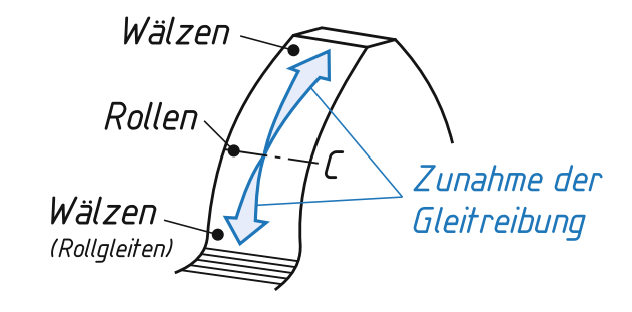
\includegraphics[width=\linewidth,keepaspectratio]{graphics/gear_rolling_process.png}
\tcblower
\textbf{\ZSFkeyword*{Spezifisches Gleiten}} $\ZSFgearSlip$:~\ZSFgapXS
{\centering $\displaystyle |\ZSFgearSlip| = \frac{\ZSFgearVSliding}{\ZSFgearVRolling} \leq 2$\par}
\ZSFgapS
Am Wälzpunkt tritt\\
reines Rollen auf, $\ZSFgearSlip = 0$.
\ZSFgapS
$|\ZSFgearSlip|$ ist maximal beim\\
Eingriffsbeginn und -Ende.
\end{splitbox}
\ZSFindex{Gleiten, spezifisches}

\SubsectionBar[sec:stirnzahnradtechnik]{Stirnzahnräder}
\ZSFindex{Stirnzahnrad}

\ZSFfig[1.0]{graphics/stirnrad_kennwerte_zahngeometrie.png}{Kennwerte Stirnrad}{}

\SubsubsectionBarOnNewColumn*{Normzahnräder}
\begin{figbox}[]
  \noindent
  \begin{minipage}[c]{0.45\linewidth}%
    \centering
    \begin{tikzpicture}[x=0.75pt, y=0.75pt, >=latex, font=\sffamily\fontsize{5.5}{6.5}\selectfont]
      % 1. Fill gear bodies
      \fill[GearObjOneColor!8] (20, 14) rectangle (60, 30);
      \fill[GearObjTwoColor!8] (50, 14) rectangle (100, 30);

      % 2. Draw solid boundaries of Gear 1 (left/top/bottom up to contact)
      \draw[thick, GearObjOneColor] (20, 14) -- (55, 14);
      \draw[thick, GearObjOneColor] (20, 30) -- (55, 30);
      \draw[thick, GearObjOneColor] (20, 14) -- (20, 30);

      % 3. Draw dashed boundaries of Gear 1 (inside Gear 2)
      \draw[thick, GearObjOneColor, dashed] (55, 14) -- (60, 14);
      \draw[thick, GearObjOneColor, dashed] (55, 30) -- (60, 30);
      \draw[thick, GearObjOneColor, dashed] (60, 14) -- (60, 30);

      % 4. Draw solid boundaries of Gear 2 (right/top/bottom from contact)
      \draw[thick, GearObjTwoColor] (55, 14) -- (100, 14);
      \draw[thick, GearObjTwoColor] (55, 30) -- (100, 30);
      \draw[thick, GearObjTwoColor] (100, 14) -- (100, 30);

      % 5. Draw dashed boundaries of Gear 2 (inside Gear 1)
      \draw[thick, GearObjTwoColor, dashed] (50, 14) -- (55, 14);
      \draw[thick, GearObjTwoColor, dashed] (50, 30) -- (55, 30);
      \draw[thick, GearObjTwoColor, dashed] (50, 14) -- (50, 30);

      % 6. Draw vertical dashed-dotted lines (pitch lines and axes)
      \draw[dashdotted, black!60, semithick] (25, 9) -- (25, 35);
      \draw[dashdotted, black!60, semithick] (40, 5) -- (40, 38);
      \draw[dashdotted, black!60, semithick] (55, 5) -- (55, 38);
      \draw[dashdotted, black!60, semithick] (75, 5) -- (75, 38);
      \draw[dashdotted, black!60, semithick] (95, 9) -- (95, 35);

      % 7. Draw solid vertical extension lines (Hilfslinien) for all dimensions
      \draw[thick, GearVarHeightHeadColor!70] (20, 14) -- (20, 7);
      \draw[thick, GearVarHeightHeadColor!70] (25, 14) -- (25, 7);
      \draw[black!40] (40, 14) -- (40, 1);
      \draw[black!40] (55, 14) -- (55, 7);
      \draw[black!40] (75, 14) -- (75, 1);
      \draw[thick, GearVarHeightHeadColor!70] (95, 14) -- (95, 7);
      \draw[thick, GearVarHeightHeadColor!70] (100, 14) -- (100, 7);

      % 8. Dimension lines with arrowheads / ticks
      \draw[<->, >=stealth, black!60] (25, 8) -- (55, 8);
      \draw[<->, >=stealth, black!60] (55, 8) -- (95, 8);
      \draw[<->, >=stealth, black!60] (40, 2) -- (75, 2);
      
      \draw[thick, GearVarHeightHeadColor] (20, 8) -- (25, 8);
      \draw[thick, GearVarHeightHeadColor] (20, 7.2) -- (20, 8.8);
      \draw[thick, GearVarHeightHeadColor] (25, 7.2) -- (25, 8.8);
      
      \draw[thick, GearVarHeightHeadColor] (95, 8) -- (100, 8);
      \draw[thick, GearVarHeightHeadColor] (95, 7.2) -- (95, 8.8);
      \draw[thick, GearVarHeightHeadColor] (100, 7.2) -- (100, 8.8);

      % 9. Draw labels inside the gear bodies
      \node[GearObjOneColor, font=\bfseries] at (40, 22) {1};
      \node[GearObjTwoColor, font=\bfseries] at (75, 22) {2};

      % 10. Draw dimension labels LAST with background masking fill
      \node[fill=\FigboxBackColor, inner sep=1.5pt] at (40, 8) {$\ZSFgearDOne$};
      \node[fill=\FigboxBackColor, inner sep=1.5pt] at (75, 8) {$\ZSFgearDTwo$};
      \node[fill=\FigboxBackColor, inner sep=1.5pt] at (57.5, 2) {$\ZSFgearAd$};

      \node[scale=0.85] at (22.5, 3.2) {$\ZSFgearHeightHead{h_{a\ZSFgearIndexOne{1}}} = \ZSFgearModule{m}$};
      \node[scale=0.85] at (97.5, 3.2) {$\ZSFgearHeightHead{h_{a\ZSFgearIndexTwo{2}}} = \ZSFgearModule{m}$};
    \end{tikzpicture}
  \end{minipage}%
  \hfill
  \begin{minipage}[c]{\dimexpr0.96\linewidth-0.45\linewidth\relax}%
    \raggedright
    \ZSFReadableOn
    \ZSFkeyword{Eingriffswinkel}:\\
    $\ZSFgearAlpha = 20^\circ$
    \ZSFgapXS

    {\centering $\displaystyle \ZSFgearAd = \frac{\ZSFgearDOne + \ZSFgearDTwo}{2} = \frac{\ZSFgearM\cdot(\ZSFgearZOne + \ZSFgearZTwo)}{2}$\par}
    \ZSFgapXS

    {\centering $\displaystyle \ZSFgearU = \ZSFgearP \cdot \ZSFgearZ = \ZSFgearD\cdot\pi$\par}
  \end{minipage}%
  \par
\end{figbox}

\phantomsection\label{formula:gear-normal-geometry}
\begin{formulabox}[Geometrie]
\[ \ZSFgearHa = \ZSFgearM \qquad \ZSFgearHf = 1,1 \dots 1,3 \cdot \ZSFgearM \qquad \ZSFgearH = \ZSFgearHa + \ZSFgearHf \]
\[ \ZSFgearDf = \ZSFgearD - 2\cdot \ZSFgearHf \qquad \ZSFgearD = \ZSFgearZ \cdot \ZSFgearM = \ZSFgearZ \cdot \dfrac{\ZSFgearP}{\pi} \]
\[ \ZSFgearDa = \ZSFgearD + 2\cdot \ZSFgearHa = \ZSFgearD + 2\cdot \ZSFgearM \qquad \ZSFgearDb =\ZSFgearD\cdot\cos\ZSFgearAlpha \]
\formulanote{%
$\ZSFgearAd$:~Null-Achsabstand $\cdot$ $\ZSFgearU$:~Umfang $\cdot$ $\ZSFgearAlpha$:~Eingriffswinkel ($20^\circ$) \\
$\ZSFgearHa$:~Kopfhöhe $\cdot$ $\ZSFgearHf$:~Fusshöhe $\cdot$ $\ZSFgearH$:~Zahnhöhe $\cdot$ $\ZSFgearM$:~Modul $\cdot$ $\ZSFgearP$:~Teilung $\cdot$ $\ZSFgearZ$:~Zähnezahl \\
$\ZSFgearD$:~Teilkreis- $\cdot$ $\ZSFgearDf$:~Fusskreis- $\cdot$ $\ZSFgearDa$:~Kopfkreis- $\cdot$ $\ZSFgearDb$:~Grundkreisdurchmesser%
}
\end{formulabox}

\ZSFindex[grenzzahnezahl]{Grenzzähnezahl}
\begin{formulabox}[Grenzzähnezahl]
\formulanoteabove{Theoretische $\ZSFgearZg$ und praktische $\ZSFgearZgPrime$ Grenzzähnezahl:}
\[ \ZSFgearZg = 17 \text{ und } \ZSFgearZgPrime = 14 \text{ für } \ZSFgearAlpha = 20° \qquad \ZSFgearZg = \frac{2}{sin^2\ZSFgearAlpha} \]
\formulanote{Die maximale Übersetzung wird mit dem kleinsten zulässigen Zahnrad (14 Zähne) und dem grössten möglichen Zahnrad erreicht.}
\end{formulabox}

\SubsubsectionBar{Profilüberdeckung}
\ZSFindex[profiluberdeckung]{Profilüberdeckung}

\begin{runintext}
Beschreibt wieviele Zähne gleichzeitig im Eingriff sind, mit Eingriffsstrecke $\ZSFgearGalpha$ und Eingriffsteilung $\ZSFgearPe$.
\end{runintext}

\begin{formulabox}
\formulasources{$\ZSFgearDa$, $\ZSFgearDb$:~Normrad \ZSFsource{aus}{formula:gear-normal-geometry}, profilversch. \ZSFsource{aus}{formula:gear-profile-shift}}
\formulanoteabove{%
Bei Schrägverzahnung: Überdeckungsformeln \ZSFref{sec:schraegverzahnung}.}
\[ \ZSFgearEpsAlpha = \frac{\ZSFgearGalpha}{\ZSFgearPe} = \frac{\frac{1}{2}\cdot(\sqrt{\ZSFgearDaOne^2-\ZSFgearDbOne^2}+\sqrt{\ZSFgearDaTwo^2-\ZSFgearDbTwo^2}) - \ZSFgearAd\cdot \sin\ZSFgearAlpha}{\pi\cdot \ZSFgearM\cdot\cos\ZSFgearAlpha} \]
\formulanote{$\ZSFgearEpsAlpha$:~Profilüberdeckung $\cdot$ $\ZSFgearGalpha$:~Eingriffsstrecke $\cdot$ $\ZSFgearPe$:~Eingriffsteilung \\ $\ZSFgearAd$:~Null-Achsabstand $\cdot$ $\ZSFgearAlpha$:~Eingriffswinkel ($20^\circ$) $\cdot$ $\ZSFgearM$:~Modul}
\end{formulabox}
\begin{statementbox}[Eigenschaften und Richtwerte]
\ZSFReadableOn
Bei grossem $\ZSFgearEpsAlpha$:~\begin{factlist}
\item vibrationsärmer und leiser
\item höhere Lebensdauer und Tragfähigkeit
\end{factlist}
\ZSFgapS
Richtwerte $\ZSFgearEpsAlpha$:~\begin{factlist}
\item \textbf{Nicht zulässig} (kein Zahnkontakt): $\ZSFgearEpsAlphaBrace < 1.0$
\item \textbf{Industriestandard}:~$1.3 \leq \ZSFgearEpsAlpha \leq 1.6$
\item \textbf{Sehr ruhiger Lauf}:~$\ZSFgearEpsAlphaBrace \geq 1.6$
\end{factlist}
\end{statementbox}

\SubsubsectionBar{Profilverschiebung}
\ZSFindex{Profilverschiebung}

\begin{runintext}
Verhältnis von aufsteigender zu absteigender Flanke (Grundkreis $\ZSFgearDb$ bis Kopfkreis $\ZSFgearDa$). Dabei ändern sich der Achsenabstand $\ZSFgearA$ und Eingriffswinkel $\ZSFgearAlpha$.
\end{runintext}

\begin{factlist}
\ZSFFact{Kleine Flanke/ viel Unterschnitt}{Geschwächter Zahnfuss durch Biegemoment}
\ZSFFact{Grosse Flanke/ wenig Unterschnitt}{Zahn wird spitz, also kein Platz für gegenüberliegenden Zahn}
\end{factlist}

\phantomsection\label{formula:gear-profile-shift}
\begin{formulabox}[Profilverschiebungsfaktor $\ZSFgearX$]
\[
\begin{array}{ll}
  \ZSFgearVplus\text{-Rad: } \ZSFgearX > 0 \ (s\uparrow, \text{Unterschnitt}\downarrow) & \quad \big| \quad \text{Null-Rad: } \ZSFgearX = 0 \\
  \ZSFgearVminus\text{-Rad: } \ZSFgearX < 0 \ (s\downarrow, \text{Unterschnitt}\uparrow) &
\end{array}
\]
\formulasep
\[ \ZSFgearX = \frac{\ZSFgearV}{\ZSFgearM} \qquad \ZSFgearDa = \ZSFgearD + 2\ZSFgearM + 2\ZSFgearV = \ZSFgearD + 2\cdot \ZSFgearM\cdot (1+\ZSFgearX) \]
\formulanote{$\ZSFgearX$:~Profilverschiebungsfaktor $\cdot$ $\ZSFgearV$:~Verschiebung (beidseitig $\Rightarrow 2\cdot \ZSFgearV$) \\ $\ZSFgearM$:~Modul $\cdot$ $\ZSFgearD, \ZSFgearDa$:~Teilkreis-/Kopfkreisdurchmesser}
\end{formulabox}

\SubsubsectionBar[sec:geradverzahnung]{Geradverzahnung Kräfte}
\ZSFindex{Geradverzahnung}

\begin{splitbox}[0.57]
\centering
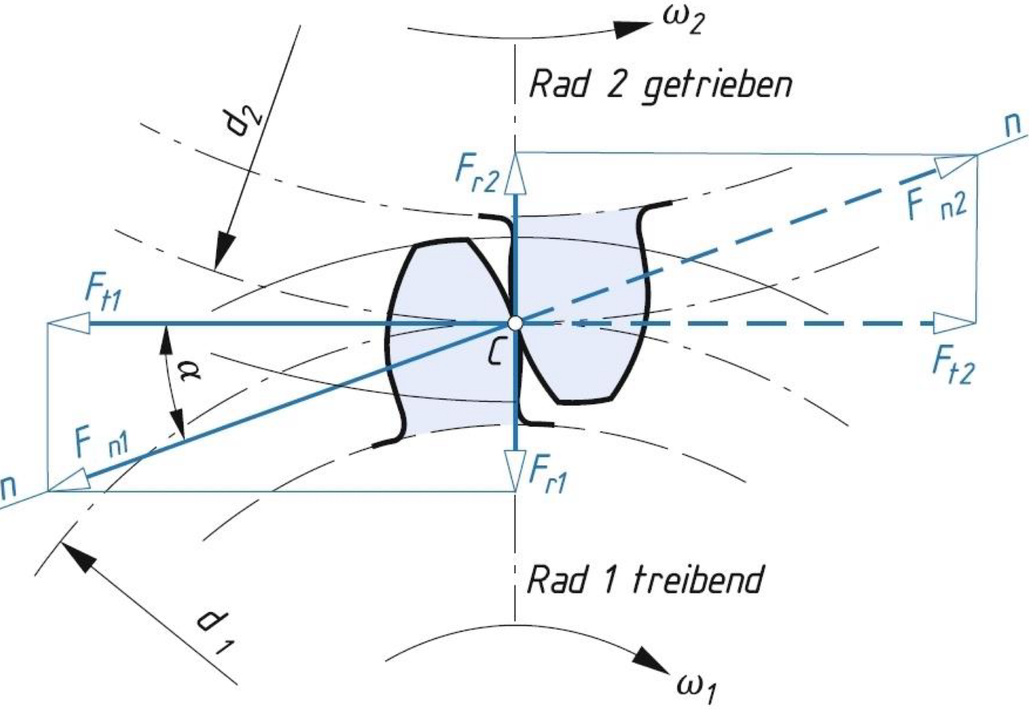
\includegraphics[width=\linewidth,keepaspectratio]{graphics/spur_gear_contact_forces_line_of_action.png}
\tcblower
Getriebenes Rad:

$\ZSFgearFtTwo = \ZSFgearFtOne$ \quad $\ZSFgearFrTwo = \ZSFgearFrOne$
\ZSFgapS

Treibendes Rad:

$\ZSFgearFtOne = \frac{\ZSFgearTorqueOne}{\ZSFgearROne} = \frac{2\cdot \ZSFgearTorqueOne}{\ZSFgearDOne}$

$\ZSFgearFrOne = \ZSFgearFtOne \cdot \tan\ZSFgearAlpha$

$\ZSFgearFn = \dfrac{\ZSFgearFt}{\cos\ZSFgearAlpha}$
\ZSFgapXS

\formulanote{%
$\ZSFgearFt$:~Tangentialkraft \\
$\ZSFgearFr$:~Radialkraft \\
$\ZSFgearFn$:~Normalkraft \\
$\ZSFgearTorque$:~Drehmoment \\
$\ZSFgearR,\ZSFgearD$:~Teilkreis- $r,d$ \\
$\ZSFgearAlpha$:~Eingriffswinkel ($20^\circ$) \\
bei Welle siehe \ZSFref{sec:biegung}%
}
\end{splitbox}

\begin{statementbox}[Kraftrichtung]
Antrieb: $\ZSFgearFrOne$ nach innen zum Antrieb, $\ZSFgearFtOne$ entgegen der Drehrichtung, $\ZSFgearFrTwo$ und $\ZSFgearFtTwo$ entgegen der $\ZSFgearFOne$ Kräfte
\end{statementbox}

\SubsubsectionBarOnNewColumn{V-Getriebe}
\ZSFindex{V-Getriebe}

\begin{runintext}
$\sum \ZSFgearX \neq 0$ und $\ZSFgearAlpha$ wird zum \ZSFkeyword{Betriebswinkel} $\ZSFgearAlphaW$.
\end{runintext}

\begin{figbox}[V-Getriebe]
  \noindent
  \begin{minipage}[c]{0.68\linewidth}
    \raggedright
    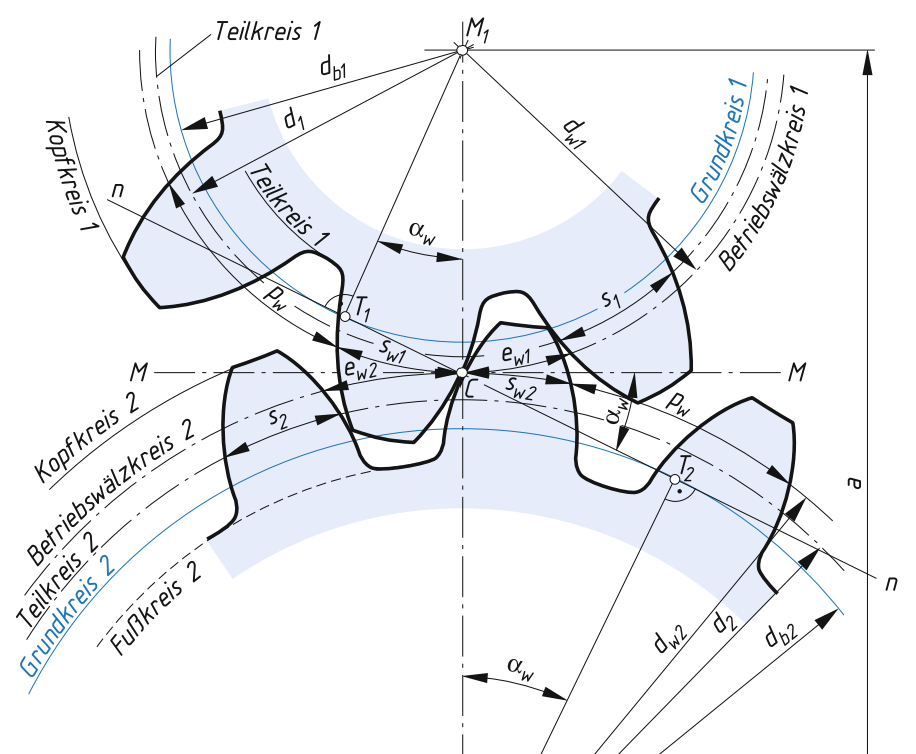
\includegraphics[width=\linewidth,keepaspectratio]{graphics/v_getriebe_kennwerte.png}
  \end{minipage}%
  \begin{minipage}[c]{0.31\linewidth}
    \centering
    $\ZSFgearSwOne = \ZSFgearEwTwo$, $\ZSFgearSwTwo = \ZSFgearEwOne$ \\[2pt]
    $\ZSFgearA = \ZSFgearAd \cdot\frac{\cos\ZSFgearAlpha}{\cos\ZSFgearAlphaW} = \ZSFgearAd + \Delta{\ZSFgearA}$ \\[3pt]
    {\ZSFfontNote $\ZSFgearSw/\ZSFgearEw$:~Wälzzahndicke/-lücke \\ $\ZSFgearA,\ZSFgearAd$:~Betriebs-/Null-Achsabstand \\ $\ZSFgearAlphaW$:~Betriebseingriffswinkel \\ $\Delta\ZSFgearA$:~Achsabstandsänderung\par}
  \end{minipage}
\end{figbox}

\begin{defbox}[Bestimmung Betriebswinkel $\ZSFgearAlphaW$]
\begin{enumerate}[leftmargin=1.1em,itemsep=0.5pt,topsep=1.5pt,parsep=0pt]
  \item $\text{inv}\,\ZSFgearAlpha = \tan\ZSFgearAlpha - \ZSFgearAlpha\cdot(\frac{\pi}{180°})$ \hfill (\small$\text{inv}\,(20°) = 0.0149$)
  \item $\text{inv}\,\ZSFgearAlphaW = 2\,\frac{\ZSFgearXOne+\ZSFgearXTwo}{\ZSFgearZOne+\ZSFgearZTwo}\,\cdot \tan\ZSFgearAlpha + \text{inv}\,\ZSFgearAlpha$
  \item $\ZSFgearAlphaW \approx (\sqrt[3]{3 \cdot \text{inv}\,\ZSFgearAlphaW} - \frac{2}{5}\text{inv}\,\ZSFgearAlphaW)\cdot (\frac{180°}{\pi})$
\end{enumerate}
\ZSFgapS
\textbf{Umgestellt:}
{\centering
$\sum \ZSFgearX = \dfrac{(\text{inv}\,\ZSFgearAlphaW - \text{inv}\,\ZSFgearAlpha)\cdot(\ZSFgearZOne+\ZSFgearZTwo)}{2 \cdot \tan\ZSFgearAlpha}$ \\[4pt]
$\ZSFgearAlphaW = \cos^{-1}\left(\frac{\ZSFgearAd}{\ZSFgearA}\cdot \cos\ZSFgearAlpha\right)$ \par}
\formulanote{$\ZSFgearAlpha$:~Eingriffswinkel ($20^\circ$) $\cdot$ $\ZSFgearAlphaW$:~Betriebseingriffswinkel \\ $\sum \ZSFgearX$:~Summe Profilverschiebung $\cdot$ $\ZSFgearZ$:~Zähnezahl}
\end{defbox}

\SubsubsectionBar{V-Null-Getriebe}
\ZSFindex{V-Null-Getriebe}

\begin{formulabox}
\[ \ZSFgearAd = \ZSFgearA = \frac{\ZSFgearDOne + \ZSFgearDTwo}{2} = \ZSFgearROne + \ZSFgearRTwo \text{ und } \sum \ZSFgearX = 0 \]
\formulanote{$\ZSFgearAd, \ZSFgearA$:~Null-/Betriebsachsabstand $\cdot$ $\ZSFgearD, \ZSFgearR$:~Teilkreisdurchmesser/-radius \\ $\ZSFgearX$:~Profilverschiebung $\cdot$ $\ZSFgearS$:~Zahndicke}
\formulanote{$\sum \ZSFgearX=0\Rightarrow \ZSFgearA=\ZSFgearAd,\ZSFgearAlphaW=\ZSFgearAlpha$; $\ZSFgearXOne>0\Rightarrow \ZSFgearSOne\uparrow$, Unterschnitt $\downarrow$; $\ZSFgearXTwo=-\ZSFgearXOne\Rightarrow \ZSFgearSTwo\downarrow$}
\end{formulabox}

\ZSFfig[1.0]{graphics/v_null_gears_characteristics.png}{V-Null-Räder}{} % chktex 25

\SubsubsectionBar[sec:schraegverzahnung]{Schrägverzahnung}
\ZSFindex[schragverzahnung]{Schrägverzahnung}

\begin{runintext}
Durch den \ZSFkeyword{Schrägungswinkel} $\ZSFgearBeta$ sind immer mehrere Zähne durch kontinuierliches Anlegen und Ablösen im Eingriff, anders als bei der Geradverzahnung. Dies ermöglicht einen kontinuierlichen Krafteinfluss und somit höhere Laufruhe und Belastbarkeit.
\end{runintext}

\begin{figbox}[Schrägverzahnung]
\centering
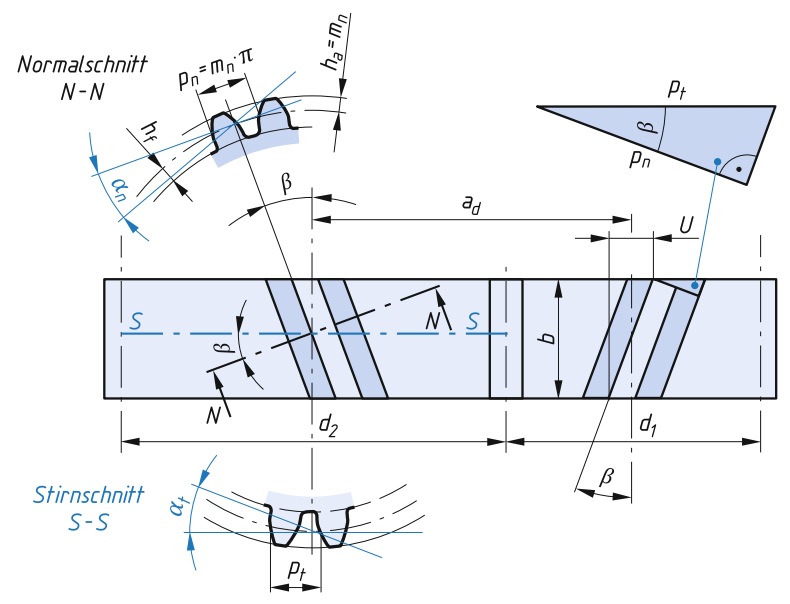
\includegraphics[width=0.73\linewidth,keepaspectratio]{graphics/helical_gear_characteristics.png}%
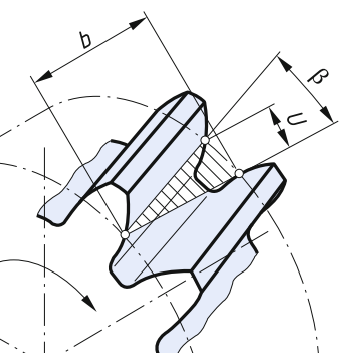
\includegraphics[width=0.25\linewidth,keepaspectratio]{graphics/helical_gear_tooth_contact_detail.png}
\end{figbox}

\phantomsection\label{formula:gear-helical-geometry}
\begin{formulabox}[Geometrie]
\[ \ZSFgearAlphaT = \tan^{-1}(\frac{\tan\ZSFgearAlphaN}{\cos{\ZSFgearBeta}}) \qquad \cos\ZSFgearBeta = \frac{\tan\ZSFgearAlphaN}{\tan\ZSFgearAlphaT} \]
\[ \ZSFgearHa = \ZSFgearMn \qquad \ZSFgearMt = \frac{\ZSFgearMn}{\cos\ZSFgearBeta} = \frac{\ZSFgearD}{\ZSFgearZ} \]
\[ \ZSFgearD = \ZSFgearMt \cdot \ZSFgearZ = \frac{\ZSFgearZ \cdot \ZSFgearMn}{cos\ZSFgearBeta} \]
\[ \ZSFgearDb = \ZSFgearD \cdot\cos\ZSFgearAlphaT = \frac{\ZSFgearZ\cdot \ZSFgearMn \cdot \cos\ZSFgearAlphaT}{\cos\ZSFgearBeta} \]
\[ \ZSFgearDa = \ZSFgearD + 2\cdot \ZSFgearHa = \ZSFgearD + 2\cdot \ZSFgearMn = \ZSFgearMn\cdot \left(2+\frac{\ZSFgearZ}{\cos\ZSFgearBeta}\right) \]
\[ \ZSFgearDf = \ZSFgearD - 2\cdot \ZSFgearHf = \ZSFgearD - 2.5 \cdot \ZSFgearMn \qquad \ZSFgearHf = 1{,}25\cdot \ZSFgearMn \]
\[ \ZSFgearAd = \frac{\ZSFgearDOne + \ZSFgearDTwo}{2}= \ZSFgearMt\cdot\frac{\ZSFgearZOne+\ZSFgearZTwo}{2} = \frac{\ZSFgearMn}{\cos\ZSFgearBeta}\cdot\frac{\ZSFgearZOne + \ZSFgearZTwo}{2} \]
\formulanote{$\ZSFgearMn$:~Normal- / $\ZSFgearMt$:~Stirnmodul \ $\cdot$ \ $\ZSFgearBeta$:~Schrägungswinkel \ $\cdot$ \ $\ZSFgearAlphaN$:~Normal- / $\ZSFgearAlphaT$:~Stirneingriffswinkel \ $\cdot$ \ $\ZSFgearAlphaWT$:~Betriebseingriffswinkel im Stirnschnitt}
\end{formulabox}

\begin{formulabox}[Überdeckungen]
\formulasources{Geometriegrössen: \ZSFsource{aus}{formula:gear-helical-geometry}}
\formulanoteabove{Null-Schrägverzahnung:}
\[ \ZSFgearEpsAlpha = \frac{\ZSFgearGalpha}{\ZSFgearPe} = \frac{\frac{1}{2}\cdot(\sqrt{\ZSFgearDaOne^2-\ZSFgearDbOne^2}+\sqrt{\ZSFgearDaTwo^2-\ZSFgearDbTwo^2}) - \ZSFgearAd\cdot \sin\ZSFgearAlphaT}{\pi\cdot \ZSFgearMt\cdot\cos\ZSFgearAlphaT} \]
\formulanoteabove{V-Schrägverzahnung:}
\[ \ZSFgearEpsAlpha = \frac{\ZSFgearGalpha}{\ZSFgearPe} = \frac{\frac{1}{2}\cdot(\sqrt{\ZSFgearDaOne^2-\ZSFgearDbOne^2}+\sqrt{\ZSFgearDaTwo^2-\ZSFgearDbTwo^2}) - \ZSFgearA\cdot \sin\ZSFgearAlphaWT}{\pi\cdot \ZSFgearMt\cdot\cos\ZSFgearAlphaT} \]
\end{formulabox}

% Spalten-Packung (6-Seiten-Ziel): eine Überdeckungs-Box in zwei geteilt,
% damit die Teile an Spaltenenden umbruchfähig sind. Inhalt unverändert.
\begin{formulabox}[Sprung- und Gesamtüberdeckung]
\[ \ZSFgearEpsBeta = \frac{\ZSFgearUJump}{\ZSFgearPt} = \frac{\ZSFgearB \cdot \tan\ZSFgearBeta}{\ZSFgearPt} = \frac{\ZSFgearB \cdot \tan\ZSFgearBeta}{\pi \cdot \ZSFgearMt} = \frac{\ZSFgearB \cdot \sin\ZSFgearBeta}{\pi \cdot \ZSFgearMn} \]
\[ \ZSFgearEpsGamma = \ZSFgearEpsAlpha + \ZSFgearEpsBeta \]
\end{formulabox}

% Spalten-Packung (6-Seiten-Ziel): Box geteilt. Inhalt unverändert.
\begin{formulabox}
\[ \ZSFgearA = \ZSFgearAd \cdot\frac{cos\ZSFgearAlpha}{cos\ZSFgearAlphaW} = \ZSFgearAd \cdot\frac{cos\ZSFgearAlphaT}{cos\ZSFgearAlphaWT} \]
\[ \ZSFgearC = 0{,}25\cdot \ZSFgearMn \qquad \ZSFgearUJump = \ZSFgearB \cdot \tan\ZSFgearBeta \qquad \ZSFgearZgtPrime = 14 \cdot \cos^3\!\ZSFgearBeta \]
\formulanote{$\ZSFgearC$:~Kopfspiel \ $\cdot$ \ $\ZSFgearUJump$:~Sprung \ $\cdot$ \ $\ZSFgearEpsAll$:~Profil-/Sprung-/Gesamtüberdeckung \ $\cdot$ \ $\ZSFgearZgtPrime$:~Grenzzähnezahl \ $\cdot$ \ $\ZSFgearB$:~Zahnbreite \ $\cdot$ \ $\ZSFgearPt$:~Stirnteilung}
\end{formulabox}
\ZSFindex[sprunguberdeckung]{Sprungüberdeckung}

\begin{figbox}[Kräfte an der Schrägverzahnung]
\centering
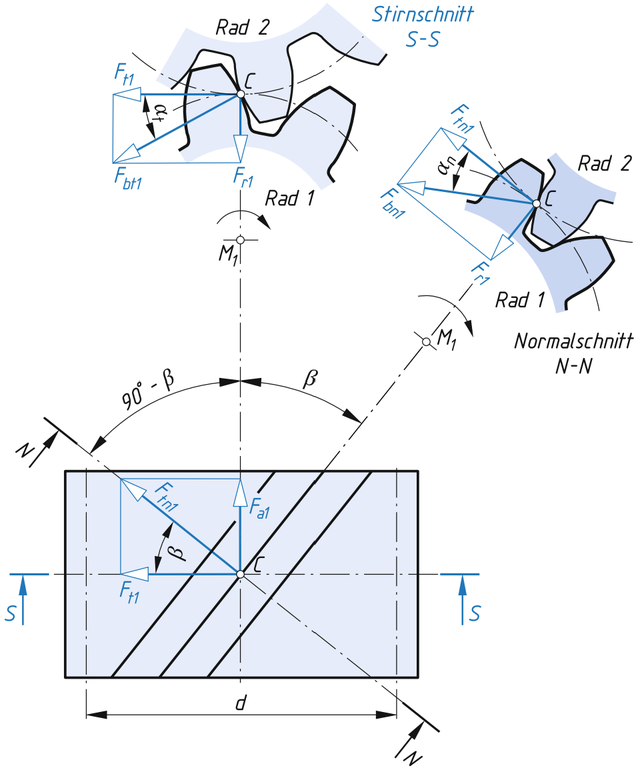
\includegraphics[width=0.62\linewidth,keepaspectratio]{graphics/helical_gear_forces.png}%
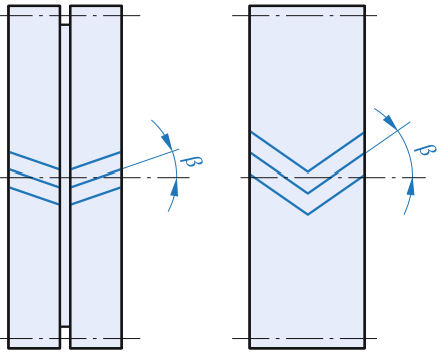
\includegraphics[width=0.38\linewidth,keepaspectratio]{graphics/helical_herringbone_gear_comparison.png}
\end{figbox}

\begin{formulabox}[Kräfte]
\[ \ZSFgearFtOne = \ZSFgearFtTwo = \frac{2\cdot \ZSFgearTorqueOne}{\ZSFgearDOne} \qquad \ZSFgearFaOne = \ZSFgearFaTwo = \ZSFgearFtOne \cdot \tan\ZSFgearBeta \]
\[ \ZSFgearFrOne = \ZSFgearFrTwo = \ZSFgearFtnOne \cdot \tan \ZSFgearAlphaN \ \text{ mit } \ \ZSFgearFtnOne = \frac{\ZSFgearFtOne}{\cos\ZSFgearBeta} \]
\formulanote{bei Welle siehe \ZSFref{sec:biegung} Biegung}
\end{formulabox}

\begin{runintext}
Axialkraft lässt sich durch Doppelschräg- oder \ZSFkeyword{Pfeilverzahnung} aufheben (siehe Bild oben).
\end{runintext}

\SubsectionBar[sec:kegelzahnradtechnik]{Kegelzahnräder}
\ZSFindex{Kegelzahnrad}
\ZSFindexsee{Kegelrad}{Kegelzahnrad}

\begin{runintext}
Umlenkung einer Drehbewegung um einen Winkel $\ZSFgearSigmaAngle$. Falls Zahnrad 1 und 2 baugleich sind: $\ZSFgearDeltaOne = \ZSFgearDeltaTwo$
\end{runintext}

\begin{formulabox}[Übersetzung und Kegelwinkel]
\[ \ZSFgearMotion{i} = \frac{\ZSFgearNOne}{\ZSFgearNTwo} = \frac{\ZSFgearDmTwo}{\ZSFgearDmOne} = \frac{\ZSFgearDeTwo}{\ZSFgearDeOne} = \frac{\ZSFgearZTwo}{\ZSFgearZOne} = \frac{\sin\ZSFgearDeltaTwo}{\sin\ZSFgearDeltaOne} = \frac{\ZSFgearTorqueTwo}{\ZSFgearTorqueOne} \]
\[ \ZSFgearSigmaAngle = \ZSFgearDeltaOne + \ZSFgearDeltaTwo \]
\end{formulabox}

\begin{formulabox}[Kegelwinkel $\ZSFgearDeltaOne$ bestimmen]
\[ \text{Für } \ZSFgearSigmaAngle \leq 90°: \ \tan\ZSFgearDeltaOne = \frac{\sin\ZSFgearSigmaAngle}{\ZSFgearMotion{i}+\cos\ZSFgearSigmaAngle} \]
\[ \text{Für } \ZSFgearSigmaAngle > 90°: \ \tan\ZSFgearDeltaOne = \frac{\sin\ (180°- \ZSFgearSigmaAngle)}{\ZSFgearMotion{i}-\cos\ (180° - \ZSFgearSigmaAngle)} \]
\end{formulabox}

\ZSFfig[0.75]{graphics/kegelradgetriebe_kennwerte_kegelradpaar.png}{Kennwerte Kegelradgetriebe}{}

\ZSFfig[0.84]{graphics/bevel_gear_pair_forces.png}{Kräfte am Kegelradpaar}{}

\begin{formulabox}[Kräfte]
\[ \ZSFgearFmtOne = \frac{2 \cdot \ZSFgearTorqueOne}{\ZSFgearDmOne} \qquad \ZSFgearFrOne = \ZSFgearFmtOne \cdot \tan\ZSFgearAlpha \cdot\cos\ZSFgearDeltaOne \]
\[ \ZSFgearFaOne = \ZSFgearFmtOne \cdot \tan\ZSFgearAlpha \cdot \sin\ZSFgearDeltaOne \]
\[ \ZSFgearFmtTwo = \ZSFgearFmtOne \qquad \ZSFgearFrTwo = \ZSFgearFmtOne\cdot \tan \ZSFgearAlpha \cdot\cos\ZSFgearDeltaTwo \]
\[ \ZSFgearFaTwo = \ZSFgearFmtOne \cdot \tan\ZSFgearAlpha \cdot \sin\ZSFgearDeltaTwo \]
\end{formulabox}

\SubsectionBar[sec:getriebe]{Getriebe}
\ZSFindex{Getriebe}

\begin{runintext}
Spannung $\Leftrightarrow$ Geometrie $\Leftrightarrow$ Kräfte
\end{runintext}

\begin{formulabox}
\[ \ZSFgearMotion{i_{ges}} = \frac{\ZSFgearNAn}{\ZSFgearNAb} \qquad \ZSFgearPsid = \frac{\ZSFgearB}{\ZSFgearDOne} = \frac{\ZSFgearB}{\ZSFgearM \cdot \ZSFgearZOne} \]
\end{formulabox}

\begin{propertylist}[Kausalität]
\ZSFFact{Welle}{Minimaler Zahnrad-Innendurchmesser $\ZSFgearDsh$}
\ZSFFact{Übersetzung}{Zähnezahlverhältnis}
\ZSFFact{Zähnezahl}{Laufruhe und Untergrenze für Modul}
\ZSFFact{Breite}{Tragfähigkeit}
\ZSFFact{Schrägung}{Laufruhe, Momente und Axialkräfte}
\ZSFFact{Modul}{Verknüpfung Zahnradgeometrie mit Materialkennwerten}
\end{propertylist}

\begin{statementbox}[Modulwahl]
\ZSFindex{Modulwahl}
\begin{factlist}
\item Keine plastische Verformungen
\item Kein statischer Bruch
\item Keine Ermüdigungsschädigung
\end{factlist}
\end{statementbox}

\begin{formulabox}[Modul-Dimensionierung]
\formulanoteabove{\textbf{Zahnfl. gehärtet:}}
\noindent $\displaystyle \ZSFgearMnTriplePrime \approx 1.85\cdot\sqrt[3]{\frac{\ZSFgearTorqueEqOne\cdot\cos^2\ZSFgearBeta}{\ZSFgearPsid\cdot \ZSFgearZOne^2\cdot\ZSFgearSigmaFlimOne}}$ \hfill {\ZSFfontNote $\ZSFgearPsid=\ZSFgearBOne/\ZSFgearDOne$}
\formulasep
\formulanoteabove{\textbf{ungehärtet bzw. vergütet:}}
\noindent $\displaystyle \ZSFgearMnTriplePrime \approx \frac{95\cdot\cos\ZSFgearBeta}{\ZSFgearZOne}\cdot\sqrt[3]{\frac{\ZSFgearTorqueEqOne}{\ZSFgearPsid\cdot\ZSFgearStrength{\sigma^2_{Hlim}}}\cdot\frac{\ZSFgearMotion{u} + 1}{\ZSFgearMotion{u}}}$ \hfill {\ZSFfontNote $\ZSFgearMotion{u} = \ZSFgearZGross/\ZSFgearZKlein$}
\formulanote{$\ZSFgearTorqueEqOne$:~äquivalentes Drehmoment an Rad 1}
\end{formulabox}

\begin{formulabox}[Spannungen und Kräfte]
\[ \ZSFgearStrength{S} = \frac{\ZSFgearStrength{R}}{\ZSFgearStrength{B}} \geq 1 \qquad \ZSFgearFt = \frac{2 \cdot \ZSFgearTorque}{\ZSFgearDOne} = \frac{2 \cdot \ZSFgearTorque}{\ZSFgearZOne \cdot \ZSFgearM} \]
\[ \ZSFgearStrength{\sigma_{zul}} \approx \frac{2 \cdot \ZSFgearTorque}{\ZSFgearPsid \cdot \ZSFgearZOne^2 \cdot \ZSFgearM^3} \]
\end{formulabox}

% Spalten-Packung (6-Seiten-Ziel): Box geteilt. Inhalt unverändert.
\begin{formulabox}
\[ \ZSFgearStrength{\sigma} = \frac{\ZSFgearF}{\ZSFgearGeom{A}} = [\frac{N}{mm^2}] = \sqrt{\frac{\ZSFgearFt}{\ZSFgearB \cdot \ZSFgearDOne}} = \ZSFgearStrength{k}\cdot\frac{\ZSFgearFt}{\ZSFgearB \cdot \ZSFgearM} \approx \frac{\ZSFgearFt}{\ZSFgearB\cdot \ZSFgearM} \]
\formulanote{$\ZSFgearStrength{B}$:~Beanspruchung \ $\cdot$ \ $\ZSFgearStrength{R}$:~Tragfähigkeit \ $\cdot$ \ $\ZSFgearStrength{k}$:~Konstante (Festigkeitsnachw.) \\
$\ZSFgearStrength{S}$:~Sicherheit \ $\cdot$ \ $\ZSFgearStrength{\sigma_{zul}}$:~Zahnfuss-Dauerfestigkeitsgrenze \\
$\ZSFgearStrength{\sigma_F}$:~Zahnfussfestigkeit (zul. Biegefestigkeit gegen Bruch am Zahnfuss) \\
$\ZSFgearStrength{\sigma_H}$:~Flankenfestigkeit (zul. Oberflächenfestigkeit gegen Fressen)}
\end{formulabox}
\ZSFindex{Zahnfussfestigkeit}
\ZSFindex{Flankenfestigkeit}

\begin{runintext}
Je grösser die Krümmung am Berührungspunkt der Flanken, desto grösser die Kräfte:~\end{runintext}

\begin{factlist}
\ZSFFact{Harter/ spröder Zahn}{Versagen am Zahnfuss (schnelle Rissbildung)}
\ZSFFact{Zäher Zahn}{Versagen an der Flanke (Elastizität der Oberfläche wirkt für den Zahnfuss dämpfend)}
\end{factlist}

\begin{defbox}[Vergütung]
\ZSFindex[vergutung]{Vergütung}
Intensives Erhitzen und schnelles, oberflächliches Abkühlen (\ZSFkeyword{Martensit}) für eine harte Oberfläche (Härtetief gegen Verschleiss) und langsames Abkühlen (\ZSFkeyword{Perlit}) für ein zäher Kern (Elastizität gegen Bruch).
\end{defbox}

\SubsubsectionBar{Planetengetriebe}
\ZSFindex{Planetengetriebe}
\ZSFindexsee{Umlaufgetriebe}{Planetengetriebe}
\ZSFindex{Sonnenrad}
\ZSFindex{Hohlrad}
\ZSFindex{Steg}

\begin{factlist}
\item Hohe Übersetzung auf kleinem Raum
\item Hoher Wirkungsgrad
\item Koaxiale Eingangs- und Ausgangswelle
\end{factlist}

\ZSFfig[1.0]{graphics/umlaufgetriebe_planetengetriebe_schema.png}{Umlaufgetriebe}{$\ZSFgearNOne$ \ZSFgearOne{Sonnenrad}; $\ZSFgearNTwo$ \ZSFgearTwo{Planetenrad}; $\ZSFgearNThree$ \ZSFgearThree{Hohlrad}; $\ZSFgearNCarrier$ \ZSFgearCarrier{Steg}}

\begin{formulabox}[Geometrie und Zähnezahlen]
\[ \ZSFgearZThree < 0\text{; Weil Hohlrad!} \qquad \ZSFgearDp = \ZSFgearDTwo \]
\[ \ZSFgearDThree = \ZSFgearD = \ZSFgearDOne + 2\cdot \ZSFgearDTwo \qquad \ZSFgearDThree = 2\cdot \ZSFgearDTwo + \ZSFgearDOne \]
\[ -\ZSFgearZThree = \ZSFgearZOne + 2\cdot \ZSFgearZTwo \qquad \mathbb{Z} = \frac{|\ZSFgearZOne| + |\ZSFgearZThree|}{\# p} \]
\end{formulabox}

\begin{formulabox}[Standübersetzung und Willis-Gleichung]
\[ \ZSFgearMotion{i_0} = \frac{\ZSFgearZThree}{\ZSFgearZOne} = \dfrac{-\ZSFgearDThree}{\ZSFgearDOne} = \dfrac{\ZSFgearNOne}{\ZSFgearNThree} = \dfrac{\ZSFgearTorqueAb}{\ZSFgearTorqueAn} \]
\formulanote{bei $\ZSFgearNCarrier = 0$; Standgetriebe}
\formulanoteabove{Willis-Gleichung:}
\[ \ZSFgearNOne - \ZSFgearNCarrier \cdot (1-\ZSFgearMotion{i_0}) - \ZSFgearMotion{i_0}\cdot \ZSFgearNThree = 0 \]
\end{formulabox}
\ZSFindex{Willis-Gleichung}

% Tabelle von luca dwellig zmf
\begin{tablebox}[Planetengetriebe: Übersetzungen]
\renewcommand{\arraystretch}{1.55}
\begin{ZSFtable}{Z{0.6} Z{0.7} Z{0.7} Z{2.0}}
\ZSFheaderRow \ZSFhead{Fest} & \ZSFhead{Ab} & \ZSFhead{An} & \ZSFhead{$\ZSFgearMotion{i}$} \\
Steg & Hohlrad & Sonne & \ZSFtablestrut $\ZSFgearMotion{i_0} = \dfrac{\ZSFgearNOne}{\ZSFgearNThree}$ \\
Steg & Sonne & Hohlrad & \ZSFtablestrut $\dfrac{1}{\ZSFgearMotion{i_0}} = \dfrac{\ZSFgearNThree}{\ZSFgearNOne}$ \\
Hohlrad & Steg & Sonne & \ZSFtablestrut $1 - \ZSFgearMotion{i_0} = \dfrac{\ZSFgearNOne}{\ZSFgearNCarrier}$ \\
Hohlrad & Sonne & Steg & \ZSFtablestrut $\dfrac{1}{1 - \ZSFgearMotion{i_0}} = \dfrac{\ZSFgearNCarrier}{\ZSFgearNOne}$ \\
Sonne & Hohlrad & Steg & \ZSFtablestrut $\dfrac{\ZSFgearMotion{i_0}}{\ZSFgearMotion{i_0} -1} = \dfrac{\ZSFgearNCarrier}{\ZSFgearNThree}$ \\
Sonne & Steg & Hohlrad & \ZSFtablestrut $1 - \dfrac{1}{\ZSFgearMotion{i_0}} = \dfrac{\ZSFgearNThree}{\ZSFgearNCarrier}$
\end{ZSFtable}
\end{tablebox}

\begin{figbox}[Sonderfälle]
\centering
$\ZSFgearNThree = 0$ \quad\qquad $\ZSFgearNOne = 0$ \qquad $\ZSFgearNOne = \ZSFgearNCarrier = \ZSFgearNThree$ \quad $\ZSFgearNCarrier = 0$\\
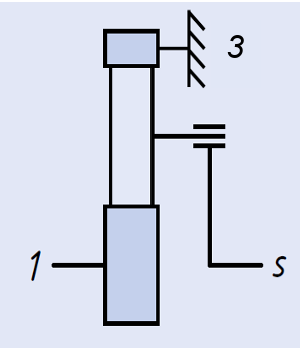
\includegraphics[width=0.23\linewidth,keepaspectratio]{graphics/v3_planetengetriebe_hohlrad_fest_n3_0.png}
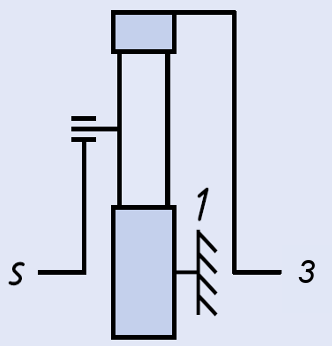
\includegraphics[width=0.25\linewidth,keepaspectratio]{graphics/v3_planetengetriebe_sonne_fest_n1_0.png}
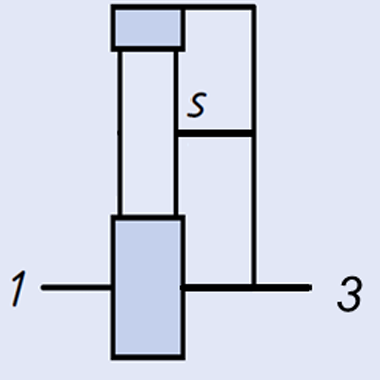
\includegraphics[width=0.24\linewidth,keepaspectratio]{graphics/v3_planetengetriebe_gleichlauf_n1_ns_n3.png}
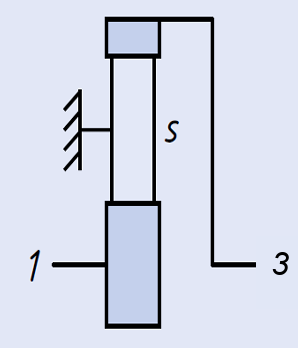
\includegraphics[width=0.23\linewidth,keepaspectratio]{graphics/v3_planetengetriebe_steg_fest_ns_0.png}
\end{figbox}

\columnbreak
% !TEX root = ../main.tex
% SECTION 2: WELLE-NABE-VERBINDUNGEN
% Inhalt: Liv Erne, Silvio Seiz — Form: ZSF-Template-Rework
% ============================================================

\StartChapter[ch:wnv]{Welle-Nabe-Verbindungen}
\ZSFindexsee{WNV}{Welle-Nabe-Verbindung}
\ZSFindex{Welle-Nabe-Verbindung}

\SubsectionBar[sec:wnv-formschluss]{Formschlüssige WNV}
\ZSFindex[formschlussige wnv]{formschlüssige WNV}

\begin{defbox}[Formschluss]
Moment wird durch \ZSFkeyword{Mitnehmerelemente} und -Geometrie übertragen. Beispiele: Zahnwelle, Polygonprofile, Längsstift, Querstift.
\end{defbox}

\begin{statementbox}[Kurzschreibweise]
DIN 6885$-$A$-10\times8\times32$\\
(DIN Norm -- Form -- Breite $\times$ Höhe $\times$ Länge)
\end{statementbox}

\SubsubsectionBar{Passfeder}
\ZSFindex{Passfeder}
\ZSFindexsee{DIN 6885}{Passfeder}

\phantomsection\label{formula:wnv-pzul}
\begin{formulabox}[Tragende Länge und Pressung]
\formulasources{$\ZSFwnvRe$:~\ZSFsource{aus}{sec:werkstoffkennwerte} \ $\cdot$ \ $\ZSFwnvS$:~\ZSFsource{aus}{sec:sicherheit}}
{\centering $\displaystyle \text{Form A (gerundet): } \ZSFwnvLt = \ZSFwnvL - \ZSFwnvB \quad \text{Form B (rechteckig): } \ZSFwnvLt = \ZSFwnvL$\par}
\formulasep
{\centering $\displaystyle \ZSFwnvPm = \frac{2 \cdot \ZSFwnvMt}{\ZSFwnvD \cdot (\ZSFwnvH-\ZSFwnvTOne)\cdot \ZSFwnvLt} = \frac{\ZSFwnvF}{\ZSFwnvA} \qquad \ZSFwnvPzul = \frac{\ZSFwnvRe}{\ZSFwnvS}$\par}
\ZSFgapXS
{\centering $\displaystyle \ZSFwnvF=\ZSFwnvFt=\frac{2\cdot \ZSFwnvMt}{\ZSFwnvD} \qquad \ZSFwnvA = \ZSFwnvHt \cdot \ZSFwnvLt = (\ZSFwnvH - \ZSFwnvTOne) \cdot \ZSFwnvLt$\par}
\end{formulabox}

\ZSFfig[0.65]{graphics/passfeder_mittlere_pressung.png}{Mittlere Pressung Passfeder}{}

\SubsubsectionBar{Keilwelle}
\ZSFindex{Keilwelle}

\begin{runintext}
Welle mit gleichmässig verteilten Keilen als Mitnehmerelemente.
\end{runintext}

\begin{formulabox}[Tragende Fläche und Pressung]
\formulasources{$\ZSFwnvLt$:~Geometrie ($\ZSFwnvLt\leq\ZSFwnvL$) \ $\cdot$ \ $\ZSFwnvPzul$:~\ZSFsource{aus}{formula:wnv-pzul}}
{\centering $\displaystyle \ZSFwnvA = \ZSFwnvLt \cdot \ZSFwnvHt \cdot \ZSFwnvN \cdot \ZSFwnvPhi \qquad \text{\TableCellNote{\dots Anzahl Keile $\ZSFwnvN$}}$\par}
\ZSFgapXS
{\centering $\displaystyle \ZSFwnvHt \approx 0,4 \cdot\frac{\ZSFwnvDbig-\ZSFwnvD}{2} \qquad \ZSFwnvH = \frac{\ZSFwnvDbig-\ZSFwnvD}{2}$\par}
\formulasep
{\centering $\displaystyle \ZSFwnvPm = \frac{10 \cdot \ZSFwnvMt}{(\ZSFwnvDbig + \ZSFwnvD)\cdot \ZSFwnvLt \cdot (\ZSFwnvDbig-\ZSFwnvD)\cdot \ZSFwnvN \cdot \ZSFwnvPhi} = \frac{\ZSFwnvF}{\ZSFwnvA} = \ZSFwnvPzul$\par}
\ZSFgapXS
{\centering $\displaystyle \ZSFwnvF = \frac{2\cdot \ZSFwnvMt}{\ZSFwnvDm} = \frac{4 \cdot \ZSFwnvMt}{\ZSFwnvDbig + \ZSFwnvD}$\par}
\end{formulabox}

\ZSFfigside[0.53]{graphics/keilwelle_zentrierungsarten.png}{Keilwelle und Zentrierungsarten}{%
  \ZSFReadableOn
  \begin{propertylist}[Tragfaktor $\ZSFwnvPhi$]
    \ZSFFact{Innenzentrierung}{Spiel an den Flanken, sehr genauer Rundlauf ($\ZSFwnvPhi = 0.75$)}
    \ZSFFact{Flankenzentrierung}{Spiel am Umfang, unempfindlich gegen Stösse ($\ZSFwnvPhi = 0.90$)}
  \end{propertylist}
}
\ZSFindex{Tragfaktor}

\SubsectionBar[sec:wnv-reibschluss]{Reibschlüssige WNV}
\ZSFindex[reibschlussige wnv]{reibschlüssige WNV}

\begin{runintext}
Moment wird durch \ZSFkeyword{Reibschluss} übertragen. Beispiele: Kegelspannelemente, Kelgelspannsatz, Schrumpfscheibe, Sternscheiben, Druckhülse, Toleranzring, Klemmverbindung, Kreiskeilverbindung.
\end{runintext}

\SubsubsectionBar[sec:zpv]{Zylindrischer Pressverband ZPV}
\ZSFindex{Pressverband, zylindrischer}
\ZSFindexsee{ZPV}{Pressverband, zylindrischer}

\begin{runintext}
Pressung, weil $\ZSFwnvDwelle > \ZSFwnvDnabe$.
\end{runintext}

\begin{figbox}[Zylindrischer Pressverband ZPV]
  \centering
  \begin{tikzpicture}[x=0.99pt, y=1pt, >=latex, font=\sffamily\fontsize{5.5}{6.5}\selectfont]
    % --- 1. Stirnansicht (left) ---
    \def\xS{28}
    \def\yS{22}
    \def\rHub{16}
    \def\rShaft{10}
    \def\rInner{5}
    
    % Fills
    \fill[fill=\chaptercolorlight!20] (\xS,\yS) circle (\rHub);
    \fill[fill=white] (\xS,\yS) circle (\rShaft);
    \fill[fill=black!6] (\xS,\yS) circle (\rShaft);
    \fill[fill=white] (\xS,\yS) circle (\rInner);
    
    % Circles
    \draw[black, thin] (\xS,\yS) circle (\rHub);
    \draw[black, thick] (\xS,\yS) circle (\rShaft);
    \draw[black, thin] (\xS,\yS) circle (\rInner);
    
    % Axes
    \draw[ultra thin, black!40, dashdotted] (\xS-19, \yS) -- (\xS+19, \yS);
    \draw[ultra thin, black!40, dashdotted] (\xS, \yS-19) -- (\xS, \yS+19);
    
    % Contact point top (28, 32)
    \coordinate (C1) at (\xS, \yS+\rShaft);
    \fill[black] (C1) circle (0.8);
    
    % FN (pointing down to contact point, head at 32, green)
    \draw[thick, MechRoleGreen, ->] (28, 44) -- (28, 32);
    \node[above, MechRoleGreen] at (28, 44) {$\ZSFwnvFN$};
    
    % Ft,max (applied tangential force, violet, pointing right, head at 28)
    \draw[thick, MechRoleViolet, ->] (12, 32) -- (28, 32);
    \node[left, MechRoleViolet] at (10, 32) {$\ZSFwnvFtMax$};
    
    % FR,t (resisting friction, amber, pointing left, head at 28)
    \draw[thick, MechRoleAmber, ->] (44, 32) -- (28, 32);
    \node[right] at (46, 32) {$\ZSFwnvFRt$};
    
    % Mt (torque arc at the outer hub edge for readability, purple)
    \draw[->, thin, MechVarMomentColor] (28, 22) ++(20:20) arc (20:70:20);
    \node[above right=-2pt, MechVarMomentColor] at (42, 38) {$\ZSFwnvMt$};
    
    % Dimension d
    \draw[ultra thin, black!50] (18, 19) -- (18, 4);
    \draw[ultra thin, black!50] (38, 19) -- (38, 4);
    \draw[<->, ultra thin, black!60] (18, 7) -- (38, 7);
    \node[below] at (28, 7) {$\ZSFwnvD$};

    % --- 2. Längsschnitt (middle) ---
    \def\xL{100}
    \def\yL{22}
    \def\wLt{28}
    
    % Stepped Shaft body with fillets (Rundungen) in the transitions
    \filldraw[fill=black!6, draw=black] 
      (81, 22) -- (81, 30) -- (83, 32) -- (114, 32) -- (114, 35) -- (120, 35) -- (120, 34) 
      to[out=270, in=180] (122, 31) -- (132, 31) -- (132, 13) -- (122, 13) 
      to[out=180, in=90] (120, 10) -- (120, 9) -- (114, 9) -- (114, 12) -- (83, 12) -- (81, 14) -- cycle;
      
    % Shaft steps/grooves representation
    \draw[black, thin] (126, 13) -- (126, 31);
    \draw[black, thin] (129, 13) -- (129, 31);
    
    % Hub halves (hatched rectangles)
    \filldraw[fill=\chaptercolorlight!20, draw=black] (86, 32) rectangle (114, 38);
    \draw[ultra thin, black!50] (88, 32) -- (94, 38);
    \draw[ultra thin, black!50] (94, 32) -- (100, 38);
    \draw[ultra thin, black!50] (100, 32) -- (106, 38);
    \draw[ultra thin, black!50] (106, 32) -- (112, 38);
    
    \filldraw[fill=\chaptercolorlight!20, draw=black] (86, 6) rectangle (114, 12);
    \draw[ultra thin, black!50] (88, 12) -- (94, 6);
    \draw[ultra thin, black!50] (94, 12) -- (100, 6);
    \draw[ultra thin, black!50] (100, 12) -- (106, 6);
    \draw[ultra thin, black!50] (106, 12) -- (112, 6);
    
    % Centerline
    \draw[ultra thin, black!40, dashdotted] (76, 22) -- (136, 22);
    
    % Contact point top (100, 32)
    \coordinate (C2) at (\xL, \yL+\rShaft);
    \fill[black] (C2) circle (0.8);
    
    % FN (pointing down to contact point, head at 32, green)
    \draw[thick, MechRoleGreen, ->] (100, 44) -- (100, 32);
    \node[above, MechRoleGreen] at (100, 44) {$\ZSFwnvFN$};
    
    % Fa,max (applied axial force, magenta, pointing right, head at 100)
    \draw[thick, MechRoleMagenta, ->] (84, 32) -- (100, 32);
    \node[above left=-1.5pt, MechRoleMagenta] at (84, 32) {$\ZSFwnvFaMax$};
    
    % FR,a (resisting friction, amber, pointing left, head at 100)
    \draw[thick, MechRoleAmber, ->] (122, 32) -- (100, 32);
    \node[above right=-1.5pt] at (122, 32) {$\ZSFwnvFRa$};
    
    % Friction coefficient and its pointer line to the contact surface
    \node[above right] at (115, 38) {$\ZSFwnvMu$};
    \draw[ultra thin, black!60] (116, 38.5) -- (109, 32);
    \fill[black!60] (109, 32) circle (0.8);
    
    % Dimension Lt (placed at the bottom to avoid top clutter)
    \draw[ultra thin, black!50] (86, 6) -- (86, -3);
    \draw[ultra thin, black!50] (114, 6) -- (114, -3);
    \draw[<->, ultra thin, black!60] (86, 0) -- (114, 0);
    \node[below] at (100, 0) {$\ZSFwnvLt$};
    
    % Dimension d
    \draw[ultra thin, black!50] (81, 32) -- (72, 32);
    \draw[ultra thin, black!50] (81, 12) -- (72, 12);
    \draw[<->, ultra thin, black!60] (74, 12) -- (74, 32);
    \node[left] at (74, 22) {$\ZSFwnvD$};

    % --- 3. Vektordreieck (right) ---
    \def\xV{155}
    \def\yV{12}
    \def\dxV{24}
    \def\dyV{17}
    
    % Ft,max (horizontal, violet)
    \draw[thick, MechRoleViolet, ->] (155, 12) -- (179, 12);
    \node[below, MechRoleViolet] at (167, 12) {$\ZSFwnvFtMax$};
    
    % Fa,max (vertical, magenta)
    \draw[thick, MechRoleMagenta, ->] (179, 12) -- (179, 29);
    \node[right, MechRoleMagenta] at (179, 20.5) {$\ZSFwnvFaMax$};
    
    % Resultant force Fres,max (hypotenuse, orange)
    \draw[very thick, MechRoleOrange, ->] (155, 12) -- (179, 29);
    \node[above left, MechRoleOrange] at (167, 20.5) {$\ZSFwnvFresMax$};
    
    % Right angle marker
    \draw (176, 12) -- (176, 15) -- (179, 15);
  \end{tikzpicture}
\end{figbox}

\begin{formulabox}[Pressung und Torsionsmoment]
\formulasources{$\ZSFwnvLt$:~Geometrie}
{\centering $\displaystyle \ZSFwnvFresMax = \sqrt{\ZSFwnvFtMax^2 + \ZSFwnvFaMax^2} \qquad \ZSFwnvFR = \ZSFwnvMu \cdot \ZSFwnvFN$\par}
\ZSFgapXS
{\centering $\displaystyle \ZSFwnvPerf = \frac{\ZSFwnvFresMax}{\ZSFwnvMu \cdot \pi \cdot \ZSFwnvD \cdot \ZSFwnvLt} \quad \text{\TableCellNote{\dots erf. Pressung}}$\par}
\formulasep
{\centering $\displaystyle \ZSFwnvMt = \frac{\ZSFwnvD \cdot \ZSFwnvFt}{2} = \frac{\ZSFwnvLt \cdot \pi \cdot \ZSFwnvD^2 \cdot \ZSFwnvPerf\cdot \ZSFwnvMu}{2}$\par}
\formulanote{Falls Zahnrad-Kraft gegeben: $\ZSFwnvFt = \ZSFgearFtTooth \cdot \frac{\ZSFgearDTooth}{\ZSFwnvD}$ (mit Zahnrad-Durchmesser $\ZSFgearDTooth$)}
\end{formulabox}


\SubsubsectionBarOnNewColumn[sec:kpv]{Kegelpressverband KPV}
\ZSFindex{Pressverband, Kegel-}
\ZSFindexsee{KPV}{Pressverband, Kegel-}

\ZSFfig[0.7]{graphics/v4_tapered_press_fit_forces.png}{Kegelpressverband}{}

\begin{formulabox}[Pressung und Kräfte]
\formulasources{$\ZSFwnvLt$:~Geometrie}
\[ \ZSFwnvDmF = \frac{\ZSFwnvDOne + \ZSFwnvDTwo}{2} \qquad \ZSFwnvFrMax = \ZSFwnvMu \cdot \ZSFwnvPerf \cdot \ZSFwnvA \]
\[ \ZSFwnvFtMax = \ZSFwnvMu \cdot \ZSFwnvPerf \cdot \pi \cdot \ZSFwnvDmF \cdot \ZSFwnvLt \qquad \tan\frac{\ZSFwnvAlpha}{2} = \frac{\ZSFwnvDOne - \ZSFwnvDTwo}{2 \cdot \ZSFwnvLt} \]
\[ \ZSFwnvPerf = \frac{2 \cdot \ZSFwnvMmax \cdot \cos\frac{\ZSFwnvAlpha}{2}}{\ZSFwnvMu \cdot \pi \cdot \ZSFwnvDmF^2 \cdot \ZSFwnvLt} \]
\[ \frac{1}{\ZSFwnvC} = \frac{\ZSFwnvDOne - \ZSFwnvDTwo}{\ZSFwnvLt} = 2 \cdot \tan\frac{\ZSFwnvAlpha}{2} \]
\formulanote{$1/\ZSFwnvC = $ Kegelverhältnis ($\ZSFwnvC = $ Kegelzahl)}
\end{formulabox}

% !TEX root = ../main.tex
% SECTION 3: BEANSPRUCHUNGEN (ACHSEN UND WELLEN)
% Inhalt: Liv Erne, Silvio Seiz — Form: ZSF-Template-Rework
% ============================================================

\StartChapter[ch:beanspruchungen]{Beanspruchungen (Achsen und Wellen)}

\SubsectionBar[sec:werkstoffkennwerte]{Werkstoffkennwerte}
\ZSFindex{Werkstoffkennwerte}
\ZSFindex{Spannungs-Dehnungs-Diagramm}

\begin{formulabox}[Spannungs-Dehnungs-Diagramm]
\[ \ZSFstressSigma = \frac{\ZSFstressF}{\ZSFstressAZero} = [\frac{N}{mm^2}] = \ZSFstressE \cdot \ZSFstressEps \qquad \ZSFstressEps = \frac{\ZSFstressDeltaL}{\ZSFstressLZero} \]
\formulanote{$\ZSFstressSigma =$ Spannung, $\ZSFstressEps =$ Dehnung}
\end{formulabox}

% Spalten-Packung (6-Seiten-Ziel): Erklaertext vor die Abbildung gezogen
% (fuellt Spaltenende); Inhalt unverändert.
\begin{runintext}
Manchmal gibt es keine klare \ZSFkeyword{Streckgrenze}, die den linear elastischen Bereich vom plastischen Bereich trennt $\rightarrow \ZSFstressRe \approx \ZSFstressRpZeroTwo$
\end{runintext}

\begin{figbox}[Streckgrenze $\ZSFstressRe$ bzw. $\ZSFstressRpZeroTwo$]
\centering
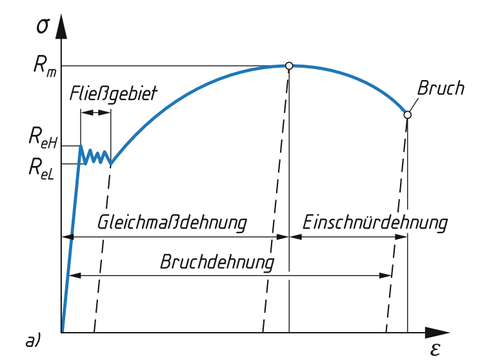
\includegraphics[width=0.40\linewidth,keepaspectratio]{graphics/spannungs_dehnungs_diagramm_streckgrenze_re.png}%
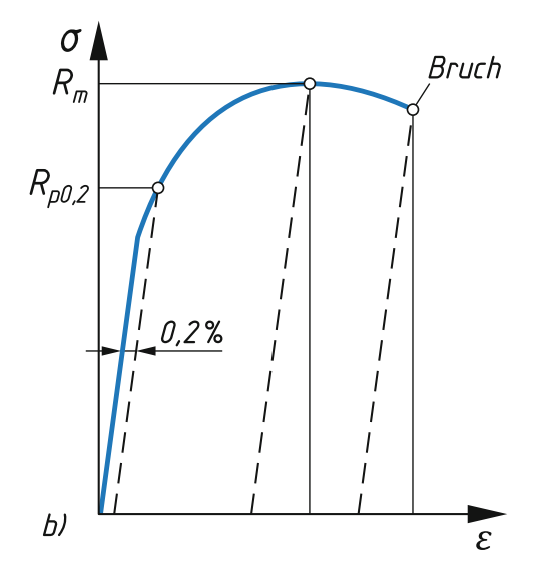
\includegraphics[width=0.30\linewidth,keepaspectratio]{graphics/spannungs_dehnungs_diagramm_dehngrenze_rp02.png}
\end{figbox}
\ZSFindex{Streckgrenze}

\SubsubsectionBar{Werkstofftabelle $\ZSFstressKt = $ Korrekturfaktor}
\ZSFindex{Korrekturfaktor}

\begin{splitbox}[0.51]
\centering
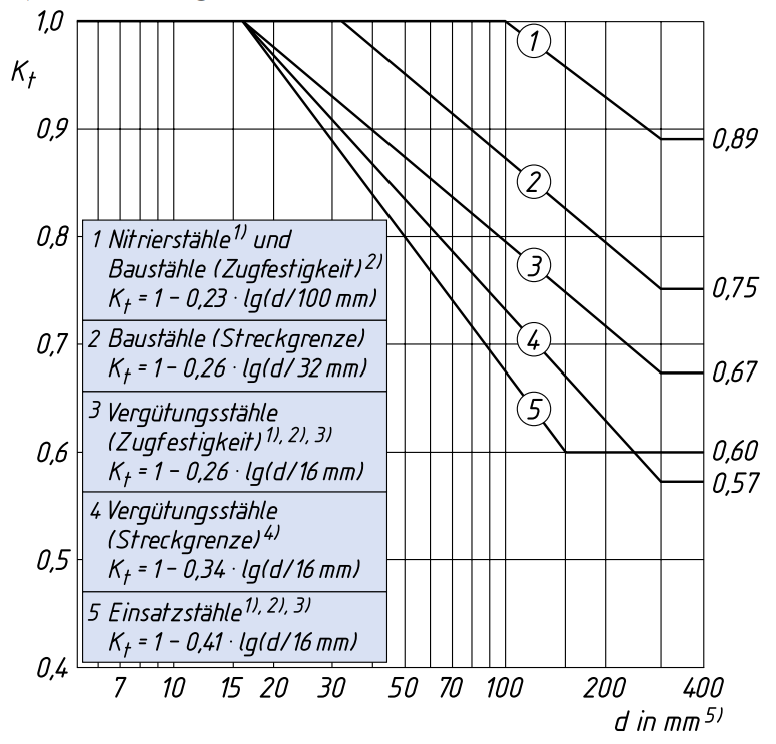
\includegraphics[width=\linewidth,keepaspectratio]{graphics/kt_size_factor_diagram.png}
\tcblower
\ZSFReadableOn
$\ZSFstressKt=1$ bis zu einem\\
bestimmten Durchmesser $\ZSFstressD$,\\
danach $\ZSFstressKt < 1$.
\ZSFgapM

{\centering $\displaystyle \ZSFstressSigmaBW=\ZSFstressKt\cdot\ZSFstressSigmaBWN$\par}
\ZSFgapXS
{\centering $\displaystyle \ZSFstressRe = \ZSFstressKt \cdot \ZSFstressReN$\par}
\ZSFgapXS
{\centering $\displaystyle \ZSFstressRm = \ZSFstressKt \cdot \ZSFstressRmN$\par}
\ZSFgapM

\formulanote{%
  $\ZSFstressSigmaBW$:~Biegewechselfestigkeit\\
  $\ZSFstressRe$:~Streckgrenze\\
  $\ZSFstressRm$:~Zugfestigkeit%
}
\end{splitbox}
\ZSFindex{Biegewechselfestigkeit}
\ZSFindex{Zugfestigkeit}

\SubsectionBar[sec:momente-spannungen]{Momente und Spannungen}

\begin{runintext}
Momente und Spannungen verursacht in Achsen und Wellen durch Zug, Druck, Scherung, Biegung und Torsion.
\end{runintext}

\begin{propertylist}[Belastungsfälle]
\item Konstant
\item Periodisch (Schwellbelastung, Wechselbelastung)
\item Nicht-periodisch
\item Stossartig
\end{propertylist}
\ZSFindex[belastungsfalle]{Belastungsfälle}

\SubsectionBar[sec:sicherheit]{Sicherheit}
\ZSFindex{Sicherheit}

\begin{formulabox}
\[ \frac{Beanspruchbarkeit\ \ZSFstressSafetyR}{Beanspruchung\ \ZSFstressSafetyB} = \frac{ertragbare\ Spannung}{vorhandene\ Spannung} \]
\end{formulabox}

\begin{runintext}
Ideal: $\ZSFstressSafetyR=\ZSFstressSafetyB$ also $\ZSFstressS=1$ \ZSFmuted{$\dots$Sicherheit} $\rightarrow$ Bauteil ist maximal ausgelastet und hält den Belastung stand.
\ZSFdanger{Aber: Keine Reserven für Unsicherheiten} (Gefügefehler, Eigenspannungen, Toleranzen und Fehlbedienungen).
\end{runintext}

\SubsectionBarOnNewColumn[sec:widerstandsmoment]{Widerstandsmoment}
\ZSFindex{Widerstandsmoment}

\begin{tablebox}[Widerstandsmoment $\ZSFstressW$]
\renewcommand{\arraystretch}{1.2}
\begin{ZSFtable}[\ZSFfontTableDense]{Z{1.3} Z{0.925} Z{0.925} Z{0.925} Z{0.925}}
  \ZSFheaderRow
  \ZSFhead{Wellenquerschnitt} & \multicolumn{2}{c}{\ZSFhead{Biegung}} & \multicolumn{2}{c}{\ZSFhead{Torsion}} \\
  \ZSFheaderRow
  & \ZSFhead{$\ZSFstressIb$} & \ZSFhead{$\ZSFstressWb$} & \ZSFhead{$\ZSFstressIt$} & \ZSFhead{$\ZSFstressWt$} \\
  \ZSFtablestrut
  \begin{tikzpicture}[scale=0.38, baseline=-0.12cm]
    \draw[dashdotted, thin, gray] (-1.1,0) -- (1.1,0);
    \draw[dashdotted, thin, gray] (0,-1.1) -- (0,1.1);
    \draw[thick, fill=gray!20] (0,0) circle (0.6);
    \draw[thin, blue] (0.6, 0.6) -- (1.1, 0.6);
    \draw[thin, blue] (0.6, -0.6) -- (1.1, -0.6);
    \draw[<->, >=stealth, thin, blue] (0.9, -0.6) -- (0.9, 0.6) node[midway, right=-1pt] {$\ZSFstressD$};
  \end{tikzpicture}
  & $\frac{\pi}{64} \cdot \ZSFstressD^4$ & $\frac{\pi}{32} \cdot \ZSFstressD^3$ & $\frac{\pi}{32} \cdot \ZSFstressD^4$ & $\frac{\pi}{16} \cdot \ZSFstressD^3$ \\
  \ZSFtablestrut
  \begin{tikzpicture}[scale=0.38, baseline=-0.12cm]
    \draw[dashdotted, thin, gray] (-1.1,0) -- (1.1,0);
    \draw[dashdotted, thin, gray] (0,-1.1) -- (0,1.1);
    \draw[thick, fill=gray!20, even odd rule] (0,0) circle (0.6) (0,0) circle (0.35);
    % d on the left
    \draw[thin, blue] (-0.35, 0.35) -- (-1.1, 0.35);
    \draw[thin, blue] (-0.35, -0.35) -- (-1.1, -0.35);
    \draw[<->, >=stealth, thin, blue] (-0.9, -0.35) -- (-0.9, 0.35) node[midway, left=-1.5pt] {$\ZSFstressD$};
    % D on the right
    \draw[thin, blue] (0.6, 0.6) -- (1.1, 0.6);
    \draw[thin, blue] (0.6, -0.6) -- (1.1, -0.6);
    \draw[<->, >=stealth, thin, blue] (0.9, -0.6) -- (0.9, 0.6) node[midway, right=-1pt] {$\ZSFstressDbig$};
  \end{tikzpicture}
  & $\frac{\pi}{64} \cdot (\ZSFstressDbig^4 - \ZSFstressD^4)$ & $\frac{\pi}{32} \cdot \frac{\ZSFstressDbig^4 - \ZSFstressD^4}{\ZSFstressDbig}$ & $\frac{\pi}{32} \cdot (\ZSFstressDbig^4 - \ZSFstressD^4)$ & $\frac{\pi}{16} \cdot \frac{\ZSFstressDbig^4 - \ZSFstressD^4}{\ZSFstressDbig}$ \\
\end{ZSFtable}
\formulanote{$\ZSFstressW = \ZSFstressI / e_{\max} =$ Widerstand gegen Randfaser-Spannung, $\ZSFstressI =$ geom.\ Widerstand gegen Verformung (Biegung/Torsion)}
\end{tablebox}

\SubsectionBar[sec:biegung]{Biegemoment $\ZSFstressMb$ und -Spannung $\ZSFstressSigmaB$}
\ZSFindex{Biegemoment}
\ZSFindex{Biegespannung}

\begin{runintext}
Durch Normalspannung verursacht (Zug/ Druck \ZSFref{sec:momverlaeufe}).
\end{runintext}

\begin{formulabox}
\formulasources{$\ZSFstressWb$:~\ZSFsource{bestimmen mit}{sec:widerstandsmoment} \ $\cdot$ \ Momentenverlauf: \ZSFsource{bestimmen mit}{sec:momverlaeufe}}
\[ \ZSFstressMb = \ZSFstressF \cdot \ZSFstressApos \qquad \ZSFstressSigmaB = \frac{\ZSFstressMb}{\ZSFstressWb} \]
\[ \ZSFstressSigmaB = \frac{32 \cdot \ZSFstressMb}{\pi \cdot \ZSFstressD^3} \]
\formulanote{$\ZSFstressApos$:~Hebelarm bzw. Position der Kraft ab Lager A}
\formulanoteabove{Max.\ Biegemoment bei 2 Lagern (Kraft bei $\ZSFstressApos$):}
\[ \ZSFstressMbMax = \frac{\ZSFstressApos\,(\ZSFstressL-\ZSFstressApos)}{\ZSFstressL}\cdot\sqrt{\ZSFstressFt^2 + \ZSFstressFr^2} \]
\ZSFgapXS
\centering
\begin{tikzpicture}[x=1pt, y=1pt, >=latex, font=\sffamily\fontsize{5.5}{6.5}\selectfont]
  \def\wL{115}
  \def\aPos{42}
  \def\leftS{8}
  \def\rightS{107}

  % Hilfslinien fuer Bemassung (sehr duenn, grau)
  \draw[ultra thin, gray, dashed] (\leftS, 6) -- (\leftS, -26);
  \draw[ultra thin, gray, dashed] (\aPos, 6) -- (\aPos, -26);
  \draw[ultra thin, gray, dashed] (\rightS, 6) -- (\rightS, -26);

  % 1. Biegemomentenverlauf
  % Momenten-Flaeche
  \fill[fill=\chaptercolorlight!40] (\leftS, -3) -- (\aPos, -10) -- (\rightS, -3) -- cycle;
  % Null-Linie
  \draw[thick, gray] (\leftS, -3) -- (\rightS, -3);
  % Verlauf
  \draw[very thick, \chaptercolor] (\leftS, -3) -- (\aPos, -10) -- (\rightS, -3);
  % Beschriftung Momentenverlauf
  \node[right, \chaptercolor, font=\sffamily\fontsize{4}{5}\selectfont] at (\rightS-22, -6.5) {$\ZSFstressMb(x)$};
  \node[below, \chaptercolor, inner sep=0.5pt, font=\sffamily\fontsize{4.5}{5.5}\selectfont] at (\aPos, -10) {$\ZSFstressMbMax$};

  % 2. Traeger (Welle)
  \draw[thick, fill=black!5] (\leftS, 6) rectangle (\rightS, 9);
  \draw[densely dashed, gray] (\leftS, 7.5) -- (\rightS, 7.5);

  % Lager A (Festlager)
  \draw[thick] (\leftS, 6) -- (\leftS, 4.5);
  \draw[thick, fill=white] (\leftS, 4.5) -- (\leftS-2.5, 0.5) -- (\leftS+2.5, 0.5) -- cycle;
  \draw[thick] (\leftS-3.5, 0.5) -- (\leftS+3.5, 0.5);
  \foreach \xx in {-2.5,-0.5,1.5}
    \draw (\leftS+\xx, 0.5) -- (\leftS+\xx-0.8, -1);
  \node[left, inner sep=0.5pt] at (\leftS-3.5, 2.5) {\scriptsize A};

  % Lager B (Loslager)
  \draw[thick] (\rightS, 6) -- (\rightS, 4.5);
  \draw[thick, fill=white] (\rightS, 4.5) -- (\rightS-2.5, 0.5) -- (\rightS+2.5, 0.5) -- cycle;
  \fill (\rightS-1.2, -0.8) circle (0.5);
  \fill (\rightS+1.2, -0.8) circle (0.5);
  \draw[thick] (\rightS-3.5, -1.8) -- (\rightS+3.5, -1.8);
  \node[right, inner sep=0.5pt] at (\rightS+3.5, 2.5) {\scriptsize B};

  % Kraft F_res (zeigt nach unten)
  \draw[->, very thick, \chaptercolor] (\aPos, 18) -- (\aPos, 10);
  \node[above, inner sep=0.5pt] at (\aPos, 17) {$\sqrt{\ZSFstressFt^2\!+\!\ZSFstressFr^2}$};

  % 3. Bemassung
  % a und L-a
  \draw[|<->|] (\leftS, -18) -- node[fill=white, inner sep=0.6pt] {$\ZSFstressApos$} (\aPos, -18);
  \draw[|<->|] (\aPos, -18) -- node[fill=white, inner sep=0.6pt] {$\ZSFstressL\!-\!\ZSFstressApos$} (\rightS, -18);
  % L darunter
  \draw[|<->|] (\leftS, -24) -- node[fill=white, inner sep=0.6pt] {$\ZSFstressL$} (\rightS, -24);
\end{tikzpicture}
\end{formulabox}

\SubsectionBar[sec:torsion]{Torsionsmoment $\ZSFstressMt$ und -Spannung $\ZSFstressTauT$}
\ZSFindex{Torsionsmoment}
\ZSFindex{Torsionsspannung}

\begin{runintext}
Durch Schubspannungen verursacht (Verschiebung).
\end{runintext}

\begin{splitbox}[0.57][sidebyside align=center]
\formulasources{$\ZSFstressWt$:~\ZSFsource{bestimmen mit}{sec:widerstandsmoment}}
{\centering $\displaystyle \ZSFstressMt = \ZSFstressF \cdot \ZSFstressR \qquad \ZSFstressTauT = \frac{\ZSFstressMt}{\ZSFstressWt}$\par}
\ZSFgapS
{\centering kreisförmiger Vollquerschnitt:\par}
\ZSFgapS
{\centering $\displaystyle \ZSFstressTauT = \frac{16 \cdot \ZSFstressMt}{\pi \cdot \ZSFstressD^3}$\par}
\tcblower
\centering
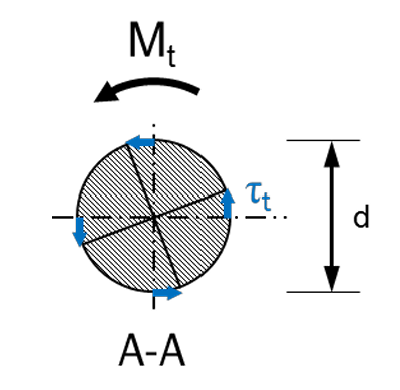
\includegraphics[width=0.6\linewidth,keepaspectratio]{graphics/v5_torsionsspannung_welle.png}
\end{splitbox}

\begin{formulabox}[Zulässige Torsionsspannung $\ZSFstressTauTzul$]
\[ \ZSFstressDmin = \sqrt[3]{\frac{16\cdot \ZSFstressMt}{\pi \cdot \ZSFstressTauTzul}} \qquad \ZSFstressTauTzul = \frac{16\cdot \ZSFstressMt}{\pi \cdot \ZSFstressDmin^3} = \frac{\ZSFstressTauTWN}{\ZSFstressSD} \]
\formulanote{\ZSFReadableOn mit Torsionswechselfestigkeit $\ZSFstressTauTWN$ und Sicherheit gegen Dauerbruch $\ZSFstressSD$}
\end{formulabox}

\begin{valuegridcustom}{l X[l]}[$\ZSFstressSD$]
\textbf{3} & Kurze und dünne Welle, keine Kerben, keine Stösse \\
\textbf{4} & Lange und dicke Welle, viele Kerben, starke Stösse
\end{valuegridcustom}

\SubsectionBar[sec:vergleichsspannung]{Vergleichsspannung $\ZSFstressSigmaV$}
\ZSFindex{Vergleichsspannung}

\begin{runintext}
Bei Kombination von Torsion und Biegung \ZSFref{sec:momverlaeufe}. Damit die Welle nicht zerbricht:
\end{runintext}

\begin{formulabox}
\formulasources{$\ZSFstressSigmaB$:~\ZSFsource{aus}{sec:biegung} \ $\cdot$ \ $\ZSFstressTauT$:~\ZSFsource{aus}{sec:torsion}}
\[ \ZSFstressSigmaV = \sqrt{\ZSFstressSigma^2 + 3\cdot   \ZSFstressTau^2} \qquad \ZSFstressSigmaV < \ZSFstressSigmaBWN \]
\[ \ZSFstressSigma= \ZSFstressSigmaRes = \ZSFstressSigmaZd + \ZSFstressSigmaB \qquad \ZSFstressTau = \ZSFstressTauRes = \ZSFstressTauS + \ZSFstressTauT \]
\formulanote{$\ZSFstressSigmaZd$:~Zug-/Druckspannung \ $\cdot$ \ $\ZSFstressTauS$:~Scherspannung}
\end{formulabox}

%\ZSFmuted{
%Schubspannungshypothese: $\sigma_v = \sqrt{\sigma^2 + 4\cdot   \tau^2}$
%Normalspannungshypothese: $\sigma_v = 0.5 \cdot (\sigma+ \sqrt{\sigma^2 + 4\cdot   \tau^2})$
%}
%\ZSFfig{graphics/vergleichsspannung_entscheidungsbaum.png}{Vergleichsspannung}{}

\SubsectionBar[sec:kerben]{Kerben}
\ZSFindex{Kerbe}
\ZSFindex{Kerbformzahl}

\begin{runintext}
\ZSFkeyword[Kerbe]{Kerben} sind kritische Stellen, da sie hohe Momente bei kleinen Durchmessern übertragen (Mehraxialer Spannungszustand im Kerbbereich).
\end{runintext}

\begin{formulabox}
\[ \ZSFstressSigmaMax = \ZSFstressAlphaK \cdot \ZSFstressSigmaN \qquad \ZSFstressTauTMax = \ZSFstressAlphaK \cdot \ZSFstressTauN \]
\[ \ZSFstressT = \frac{\ZSFstressDbig - \ZSFstressD}{2} \]
\formulanote{$\ZSFstressAlphaK$:~Kerbformzahl \ $\cdot$ \ $\ZSFstressSigmaN$, $\ZSFstressTauN$:~Nennspannung \ $\cdot$ \ $\ZSFstressT$:~Nuttiefe}
\end{formulabox}

\begin{figbox}[Kraftverteilung an Kerben]
  \centering
  $\vcenter{\hbox{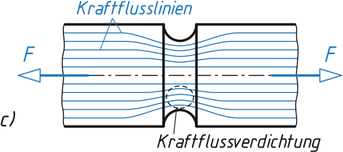
\includegraphics[width=0.25\linewidth,keepaspectratio]{graphics/kerben_split/c.png}}}$\hfill
  $\vcenter{\hbox{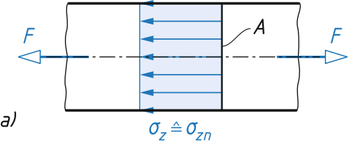
\includegraphics[width=0.25\linewidth,keepaspectratio]{graphics/kerben_split/a.png}}}$\hfill
  $\vcenter{\hbox{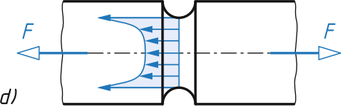
\includegraphics[width=0.25\linewidth,keepaspectratio]{graphics/kerben_split/d.png}}}$\par\ZSFgapXS
  $\vcenter{\hbox{\phantom{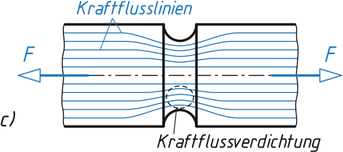
\includegraphics[width=0.25\linewidth,keepaspectratio]{graphics/kerben_split/c.png}}}}$\hfill
  $\vcenter{\hbox{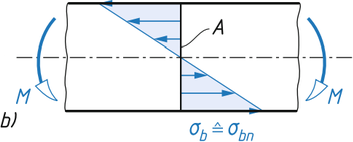
\includegraphics[width=0.25\linewidth,keepaspectratio]{graphics/kerben_split/b.png}}}$\hfill
  $\vcenter{\hbox{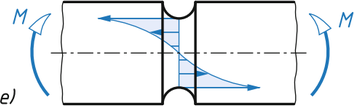
\includegraphics[width=0.25\linewidth,keepaspectratio]{graphics/kerben_split/e.png}}}$
\end{figbox}

% !TEX root = ../main.tex
% SECTION 4: TOLERANZEN
% Inhalt: Liv Erne, Silvio Seiz — Form: ZSF-Template-Rework
% ============================================================

\StartChapterOnNewColumn[ch:toleranzen]{Toleranzen}
\ZSFindex{Toleranz}

\begin{runintext}
\ZSFmuted{Bei $\ZSFtolD = 80$ wird der Tabellenabschnitt $50 - 80$ gewählt, da bis und mit gilt.}
\end{runintext}

\SubsectionBar[sec:toleranzfeldbilder]{Toleranzfeldbilder}
\ZSFindex{Toleranzfeldbild}
\ZSFindex{Passung}

\begin{runintext}
Kombinationen der Toleranzfelder von Welle und Bohrung können \ZSFkeyword[Spielpassung]{Spiel-}, \ZSFkeyword[U@Übergangspassung]{Übergangs-} und \ZSFkeyword[U@Übermasspassung]{Übermasspassungen} erzeugen:
\end{runintext}

\begin{figbox}[Spiel- / Übergangs- / Übermasspassung]
\centering
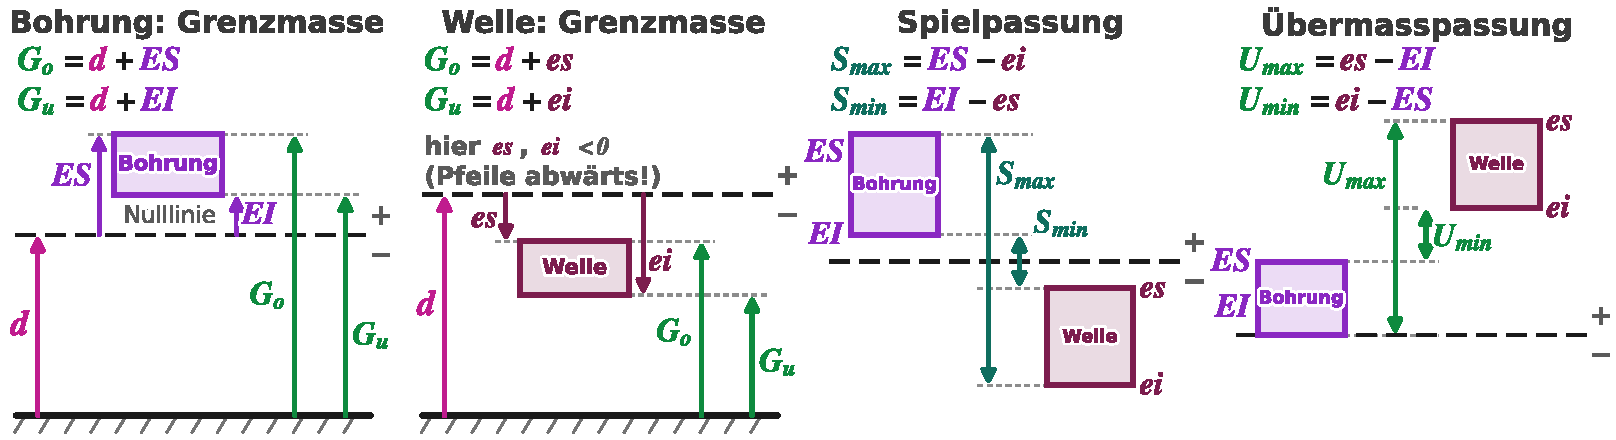
\includegraphics[width=0.88\linewidth,keepaspectratio]{graphics/toleranzfelder.pdf}
\end{figbox}

\begin{factlist}
\ZSFFact{Spielpassung}{$\ZSFtolSmin > 0 \ (\ZSFtolSmin = \ZSFtolEI - \ZSFtoles)$}
\ZSFFact{Übermasspassung}{$\ZSFtolSmax < 0 \ (\ZSFtolSmax = \ZSFtolES - \ZSFtolei)$}
\ZSFFact{Übergangspassung}{$\ZSFtolSmin < 0 < \ZSFtolSmax \ (\ZSFtolSmin = \ZSFtolEI - \ZSFtoles, \ZSFtolSmax = \ZSFtolES - \ZSFtolei)$}
\end{factlist}

%Beispiel Toleranzfeldbild:
%\ZSFfig{graphics/v6_toleranzzeichnung_welle.png}{Toleranzzeichnung Welle}{}

\begin{factlist}
\ZSFFact{Welle}{Oberes Abmass $\ZSFtoles$, unteres Abmass $\ZSFtolei$ ($\ZSFtoles > \ZSFtolei$)}
\ZSFFact{Bohrung}{Oberes Abmass $\ZSFtolES$, unteres Abmass $\ZSFtolEI$ ($\ZSFtolES > \ZSFtolEI$)}
\end{factlist}
\ZSFindex{Abmass}

\begin{formulabox}[Übermass $\ZSFtolU$ und Spiel $\ZSFtolS$]
\formulasources{$\ZSFtolUwMinMax$:~\ZSFsource{aus}{formula:tol-uw} \ $\cdot$ \ $\ZSFtolG$:~\ZSFsource{aus}{sec:rautiefe}}
\[ \ZSFtolUmin = \ZSFtolUwMin + \ZSFtolG = \ZSFtolei - \ZSFtolES = \ZSFtolei - (\ZSFtolEI + \ZSFtolIT) \]
\[ \ZSFtolUmax = \ZSFtolUwMax + \ZSFtolG = \ZSFtoles - \ZSFtolEI = (\ZSFtolei + \ZSFtolIT) - \ZSFtolEI \]
\[ \ZSFtolSmin = \ZSFtolEI - \ZSFtoles \qquad \ZSFtolSmax = \ZSFtolES - \ZSFtolei \]
\formulasep
\[ \ZSFtolEI = \ZSFtolES - \ZSFtolIT \qquad \ZSFtolei = \ZSFtoles - \ZSFtolIT \]
\formulanote{$\ZSFtolUwMinMax$:~wirksames Übermass \ $\cdot$ \ $\ZSFtolG$:~Glättung}
\end{formulabox}

\begin{figbox}[Toleranzen]
\centering
$\vcenter{\hbox{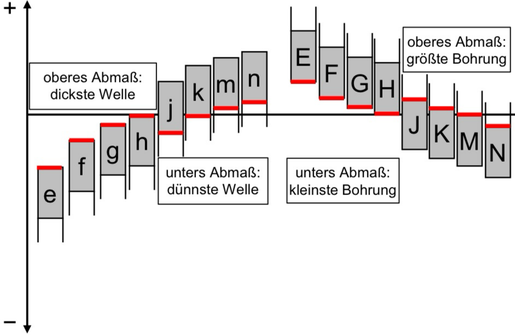
\includegraphics[width=0.62\linewidth,keepaspectratio]{graphics/toleranzfeld_lage_abmasse.png}}}%
\vcenter{\hbox{\begin{minipage}[c]{0.34\linewidth}
\centering
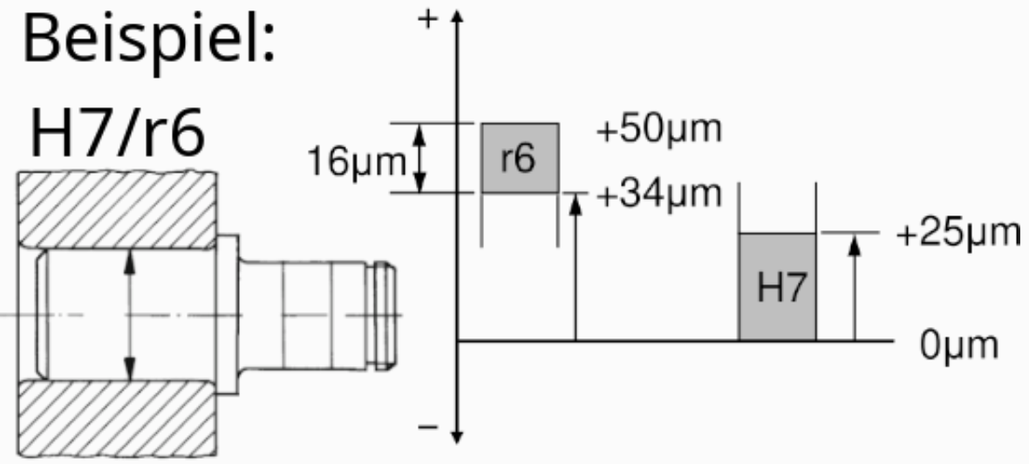
\includegraphics[width=\linewidth,keepaspectratio]{graphics/toleranzen_beispiel_h7r6.png}

\ZSFgapS
{\ZSFReadableOn Grundtoleranzgrade $\ZSFtolIT$ (Nummer nach Buchstabe) bestimmt wie gross das \textcolor{HighlightRed}{Feld} ist.\par}
\end{minipage}}}$
\end{figbox}

\phantomsection\label{formula:tol-uw}
\begin{formulabox}[Wirksames Übermass]
\formulasources{$p_{\min}$:~\ZSFsource{aus}{sec:zpv} oder \ZSFsource{aus}{sec:kpv}}
\formulanoteabove{%
$p_{\max}$:~Grenze aus zulässiger Bauteilspannung.}
\[ \ZSFtolUwMinMax = \dfrac{\ZSFtolPMinMax \cdot \ZSFtolDF}{\ZSFtolEA} \cdot \ZSFtolK \]
\formulanote{$\ZSFtolPMinMax$:~min./max. Fugenpressung \ $\cdot$ \ $\ZSFtolK$:~Hilfsgrösse \ $\cdot$ \ $\ZSFtolDF$:~Fugendurchmesser \ $\cdot$ \ $\ZSFtolEA$:~E-Modul des Aussenteils (Nabe)}
\end{formulabox}
\ZSFindex[ubermass, wirksames]{Übermass, wirksames}

\begin{warnbox}[Übermass vs. Spiel]
\ZSFconclusion{Zerbrechen bei zu grossem Übermass (Spannungen)}

\ZSFconclusion{Durchrutschen bei zu viel Spiel (keine Drehmomentübertragung)}
\end{warnbox}

\SubsectionBar[sec:hooke]{Hooke'sches Gesetz}
\ZSFindex{Hooke'sches Gesetz}

\begin{formulabox}
\formulasources{$\ZSFtolE$:~\ZSFsource{aus}{sec:werkstoffkennwerte}}
\[ \ZSFtolSigma = \ZSFtolE \cdot \ZSFtolEps = \ZSFtolE \cdot \dfrac{\ZSFtolDeltaL}{\ZSFtolL} \qquad \ZSFtolDeltaL = \dfrac{\ZSFtolSigma \ZSFtolL}{\ZSFtolE} \qquad \ZSFtolDeltaD = \dfrac{\ZSFtolP \cdot \ZSFtolDF}{\ZSFtolEA} \cdot \ZSFtolK \]
\formulasep
\formulanoteabove{Unter Temperatureinfluss:}
\[ \ZSFtolDeltaL = \ZSFtolAlpha \cdot \ZSFtolL \cdot \ZSFtolDeltaT \]
\formulanote{mit Wärmeausdehnungskoeffizient $\ZSFtolAlpha$ in $\dfrac{1}{10^{-6}K}$.}
\end{formulabox}
\ZSFindex[warmeausdehnung]{Wärmeausdehnung}

\begin{runintext}
Andernfalls kann eine Kerbe mit Gummiring eingefügt werden, um das zusätzliche Spiel durch den Temperatureinfluss zu dämpfen.
\end{runintext}

\SubsectionBar[sec:rautiefe]{Gemittelte Rautiefe $\ZSFtolRz$ und Glättung $\ZSFtolG$}
\ZSFindex{Rautiefe}
\ZSFindex[glattung]{Glättung}

\begin{runintext}
Gestaltabweichungen (Formabweichungen, Welligkeit, Riefen und Rillen) werden beim Fügevorgang geglättet.
\end{runintext}

\ZSFfigside[0.60]{graphics/v6_surface_roughness_smoothing.png}{Glättung}{%
  \ZSFReadableOn
  {\centering $\displaystyle \ZSFtolRz = \dfrac{\ZSFtolZone + \ZSFtolZtwo + \cdots + \ZSFtolZn}{\ZSFtolN}$ \par}
  \ZSFgapS
  {\centering $\displaystyle \ZSFtolG = 0.4\cdot(\ZSFtolRzA + \ZSFtolRzI)$ \par}
}

\SubsectionBarOnNewColumn[sec:genauigkeit]{Genauigkeit}
\ZSFindex{Genauigkeit}
\ZSFindex[prazision]{Präzision}
\ZSFindex{Richtigkeit}

\begin{propertylist}[Genauigkeit]
\ZSFFact{Richtigkeit}{Nähe vom Mittelwert ($\ZSFtolMu$) zum Sollwert (Zielwert) $\rightarrow$ Systematische Fehler (Im Graphen verschiebt sich die Glockenkurve nach links/ rechts)}
\ZSFFact{Präzision}{Streuung um den Mittelwert, beschrieben durch die Standardabweichung ($\ZSFtolSigma$) $\rightarrow$ Zufällige Fehler (Im Graphen flacht die Glockenkurve ab und sie wird breiter)}
\ZSFFact{Genauigkeit}{Richtigkeit und Präzision $\rightarrow$ $\ZSFtolMu =$ Sollwert, $\ZSFtolSigma$ gegen Null}
\end{propertylist}

% !TEX root = ../main.tex
% SECTION 5: FEDERN
% Inhalt: Liv Erne, Silvio Seiz — Form: ZSF-Template-Rework
% ============================================================

\StartChapter[ch:federn]{Federn}
\ZSFindex{Feder}

\begin{propertylist}[Funktionen von Federn]
\item Gewährleistung von Form- und Reibschluss
\item Speichern potentielle Energie
\item Ausgleich von Ausdehnung und Verschleiss
\item Dämpfung durch Reibung
\item Einstellen von Schwingverhalten
\end{propertylist}

\begin{figbox}[Kennlinien]
\centering
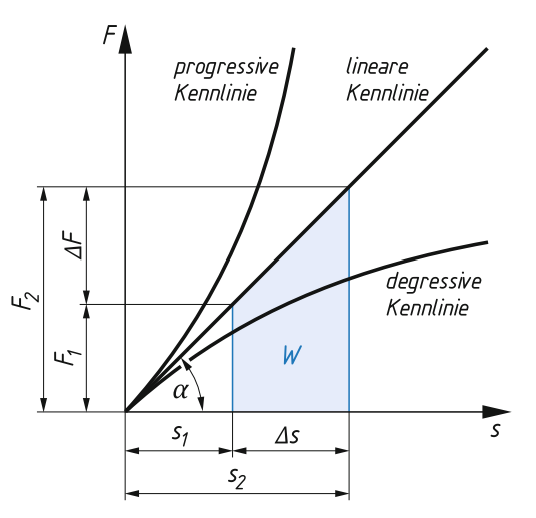
\includegraphics[width=0.5\linewidth,keepaspectratio]{graphics/schraubenfeder_kennlinie_linear_progressiv_degressiv.png}%
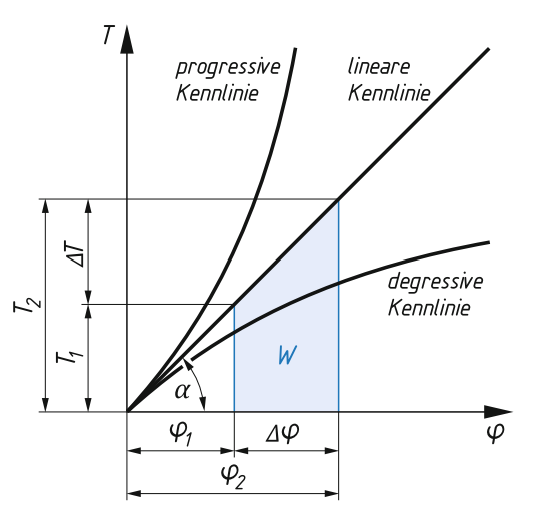
\includegraphics[width=0.5\linewidth,keepaspectratio]{graphics/drehfeder_kennlinie_linear_progressiv_degressiv.png}
\end{figbox}
\ZSFindex{Federkennlinie}

\begin{factlist}
\ZSFFact{Degressiv}{Feder wird mit steigender Belastung weicher.}
\ZSFFact{Progressiv}{Feder wird mit steigender Belastung härter.}
\end{factlist}
\ZSFgapS

\SubsectionBar{Federarbeit $\ZSFspringW$}
\ZSFindex{Federarbeit}

\begin{runintext}
Beim Spannen einer Feder wird Arbeit verrichtet, die die Feder beim Entspannen wieder abgibt. Jedoch entsteht durch die Reibung im angespannten Zustand Wärme (Dämpfungswert). Somit: $E_{Anspannen} > E_{Entspannen}$
\end{runintext}

\begin{formulabox}
\ZSFkeyword*{Federsysteme allgemein}:~$\ZSFspringW = \dfrac{1}{2}\cdot \ZSFspringF\cdot \ZSFspringS$
\formulanote{parallel: $\ZSFspringW = \dfrac{1}{2}\cdot \ZSFspringN\cdot \ZSFspringF\cdot \ZSFspringS$ mit $\ZSFspringN =$ Federn (mehrere Kräfte)}
\formulanote{in Reihe: $\ZSFspringW = \dfrac{1}{2}\cdot \ZSFspringF\cdot \ZSFspringN\cdot \ZSFspringS$ mit $\ZSFspringN =$ Federn (mehrere Wege)}
\end{formulabox}

\SubsectionBar[sec:zugdruckfedern]{Zug- und Druckfedern}
\ZSFindex{Zugfeder}
\ZSFindex{Druckfeder}

\begin{formulabox}
\ZSFkeyword*{Ersatz-Federrate $\ZSFspringRers$}: Parallelschaltung $\ZSFspringRers = \ZSFspringROne + \ZSFspringRTwo + \cdots + \ZSFspringRn$

Reihenschaltung $\ZSFspringRers = \dfrac{1}{\dfrac{1}{\ZSFspringROne} + \dfrac{1}{\ZSFspringRTwo} + \cdots + \dfrac{1}{\ZSFspringRn}}$

$\ZSFspringW = \dfrac{\ZSFspringR \cdot (\ZSFspringSTwo^2 - \ZSFspringSOne^2)}{2}\text{; } \ZSFspringWzus = \ZSFspringFv \cdot \ZSFspringDeltaS + \dfrac{1}{2}\, \ZSFspringR\, \ZSFspringDeltaS^2$
\formulanote{$\ZSFspringWzus$:~zusätzliche Federarbeit \ $\cdot$ \ $\ZSFspringFv$:~Vorspannkraft \ $\cdot$ \ $\ZSFspringDeltaS = \ZSFspringSTwo - \ZSFspringSOne$ \ $\cdot$ \ $\ZSFspringR$:~Federrate}
\formulanote{Kennlinie: je Abschnitt aktive Federn; Anschlag = aus; Steigung $\ZSFspringRers$.}
\end{formulabox}

\SubsubsectionBar{Schraubenfedern}
\ZSFindex{Schraubenfeder}

\begin{runintext}
\ZSFkeyword[Schraubenfeder]{Schraubenfedern} werden auf Torsion belastet.
\end{runintext}

\begin{figbox}[Schraubenfeder: Belastung und Geometrie]
\noindent
\begin{minipage}[c]{0.62\linewidth}
  \raggedright
  \begin{tikzpicture}[x=0.75pt,y=0.75pt,>=latex,font=\ZSFfontTableDense,every node/.style={scale=0.85}]
    % Seitenansicht: Axialkraft und Federweg
    \draw[densely dashed,gray] (30,7) -- (30,55);
    \draw[thick] (10,9) -- (50,9);
    \draw[thick] (10,51) -- (50,51);
    \draw[densely dashed,gray] (10,57) -- (50,57);
    \draw[very thick,\chaptercolor,smooth,domain=0:1440,samples=100]
      plot ({30+15*sin(\x)},{13+\x/41.15});
    \draw[->,thick,\chaptercolor] (30,63) -- (30,53) node[pos=0,left] {$\ZSFspringF$};
    \draw[->,thick,\chaptercolor] (30,-1) -- (30,7) node[pos=0,left] {$\ZSFspringF$};
    \draw[<->,thin] (6,51) -- (6,57) node[midway,left] {$\ZSFspringS$};

    % Draufsicht: Aussen-, Innen-, mittlerer und Drahtdurchmesser
    \draw[very thick,\chaptercolor] (100,29) circle (20);
    \draw[very thick,\chaptercolor] (100,29) circle (12);
    \draw[densely dashed,gray] (100,29) circle (16);
    \draw[thin] (80,49) -- (80,55);
    \draw[thin] (120,49) -- (120,55);
    \draw[<->,thin] (80,53) -- (120,53) node[midway,fill=white,inner sep=0.5pt] {$\ZSFspringDe$};
    \draw[thin] (88,9) -- (88,3);
    \draw[thin] (112,9) -- (112,3);
    \draw[<->,thin] (88,5) -- (112,5) node[midway,fill=white,inner sep=0.5pt] {$\ZSFspringDi$};
    \draw[<->,thin] (84,29) -- (116,29) node[midway,fill=white,inner sep=0.5pt] {$\ZSFspringDbig$};
    \draw[<->,thin] (100,41) -- (100,49) node[midway,right] {$\ZSFspringD$};
  \end{tikzpicture}
\end{minipage}%
\hfill
\begin{minipage}[c]{0.34\linewidth}
  \centering
  \ZSFReadableOn
  \ZSFkeyword*{Federrate}:~$\ZSFspringF = \ZSFspringR \cdot \ZSFspringS$
  \ZSFgapL
  $\displaystyle \ZSFspringDbig = \ZSFspringDi + \ZSFspringD = \ZSFspringDe -\ZSFspringD$
\end{minipage}%
\par
\ZSFgapS
\hrule
\ZSFgapS
\ZSFReadableOn
{\centering $\displaystyle \ZSFspringR = \dfrac{\ZSFspringG \cdot \ZSFspringD^4}{8 \cdot \ZSFspringDbig^3 \cdot \ZSFspringNCoils} \qquad \ZSFspringF = \dfrac{\ZSFspringG \cdot \ZSFspringD^4 \cdot \ZSFspringS}{8 \cdot \ZSFspringDbig^3 \cdot \ZSFspringNCoils}$ \par}
\ZSFgapS
{\centering $\displaystyle \ZSFspringTauT = \dfrac{\ZSFspringMt}{\ZSFspringWt} = \dfrac{16 \cdot \ZSFspringMt}{\pi \cdot \ZSFspringD^3} = \ZSFspringG \cdot \tan\ZSFspringGamma \approx \ZSFspringG \cdot \ZSFspringGamma \qquad \ZSFspringMt = \dfrac{\ZSFspringF\cdot \ZSFspringDbig}{2}$ \par}
\formulanote{$\ZSFspringG$:~Schubmodul \ $\cdot$ \ $\ZSFspringNCoils$:~aktive Windungszahl \ $\cdot$ \ $\ZSFspringGamma$:~Schubwinkel}
\end{figbox}
\ZSFindex{Federrate}

\begin{propertylist}[Gabelfedern]
\item Kleine Unebenheit $\rightarrow$ kleine Federung
\item Grosse Unebenheit $\rightarrow$ grosse Federung
\end{propertylist}
\ZSFindex{Gabelfeder}

\SubsubsectionBarOnNewColumn{Tellerfedern}
\ZSFindex{Tellerfeder}

\begin{runintext}
Halten sehr hohe Druckkräfte aus. Sie werden jedoch nie auf Block belastet ($\ZSFspringAlpha$ = 0°), weil man sonst im Bereich der plastischen Verformung ist. \ZSFdanger{Regel: $\ZSFspringS \leq 0,75 \cdot \ZSFspringHZero$}
\end{runintext}

\ZSFfig[0.65]{graphics/tellerfeder_kennwerte_abmessungen.png}{}{}
%\ZSFfig{graphics/tellerfedern_kennlinien.png}{Tellerfedern Kennlinien}{}

\begin{propertylist}[Kennlinien]
\ZSFFact{Linear}{$\ZSFspringHZero/\ZSFspringT\approx 0,4$}
\ZSFFact{Degressiv}{$\ZSFspringHZero/\ZSFspringT \approx 0,75$}
\ZSFFact{Stark degressiv (Plateau)}{$\ZSFspringHZero/\ZSFspringT \approx 1,4 \rightarrow$ Mit der Zeit verschwindet das Plateau durch Abnutzung, meistens bei Dauerbetrieb.}
\ZSFFact{Kraftmaximum erreicht}{$\ZSFspringHZero/\ZSFspringT \geq 1,4$}
\end{propertylist}

\SubsubsectionBar{Federpaket und Federsäule}
\ZSFindex{Federpaket}
\ZSFindex[federsaule]{Federsäule}

%
\ZSFfig[1.0]{graphics/tellerfeder_paket_saeule_kennlinie.pdf}{}{}

\begin{tablebox}[Paket ($\ZSFspringN$ parallel) vs. Säule ($\ZSFspringI$ in Reihe)]
\begin{ZSFtable}{Y{1.0} Y{1.0} Y{1.0}}
\ZSFheaderRow \ZSFhead{gegenüber 1 Teller} & \ZSFhead{Paket (parallel)} & \ZSFhead{Säule (Reihe)} \\
Aufbau & \ZSFtablestrut $\ZSFspringN$ Teller parallel & $\ZSFspringI$ Teller in Reihe \\
Federrate & \ZSFtablestrut $\ZSFspringRers=\ZSFspringN\cdot \ZSFspringR$ (härter) & $\ZSFspringRers=\dfrac{\ZSFspringR}{\ZSFspringI}$ (weicher) \\
bei gleichem $\ZSFspringS$:~Kraft & \ZSFtablestrut $\ZSFspringN$-fach: $\ZSFspringF\cdot \ZSFspringN$ & $\ZSFspringI$-tel: $\ZSFspringF/\ZSFspringI$ \\
bei gleichem $\ZSFspringF$:~Weg & \ZSFtablestrut $\ZSFspringN$-tel: $\ZSFspringS/\ZSFspringN$ & $\ZSFspringI$-fach: $\ZSFspringS\cdot \ZSFspringI$
\end{ZSFtable}
\formulanote{Paket teilt die Last (jeder Teller trägt $\ZSFspringF/\ZSFspringN$), Säule teilt den Weg. Gleiche Pakete ($\ZSFspringN$ parallel, $\ZSFspringI$ in Reihe): $\ZSFspringRers=\dfrac{\ZSFspringN}{\ZSFspringI}\cdot \ZSFspringR$}
\formulanote{Ungleiche Pakete in Reihe ($m$ Pakete mit $\ZSFspringN_k$ Teller): $\ZSFspringRers = \dfrac{\ZSFspringR}{\sum_{k=1}^m \frac{1}{\ZSFspringN_k}}$ \ $\cdot$ \ \ZSFdanger{Schwächstes Paket schlägt zuerst an} $\rightarrow$ Knick-Kennlinie}
\end{tablebox}

\SubsectionBar[sec:drehfedern]{Drehfedern}
\ZSFindex{Drehfeder}
\ZSFindex{Schenkelfeder}

\begin{figbox}[Schenkelfedern]
\centering
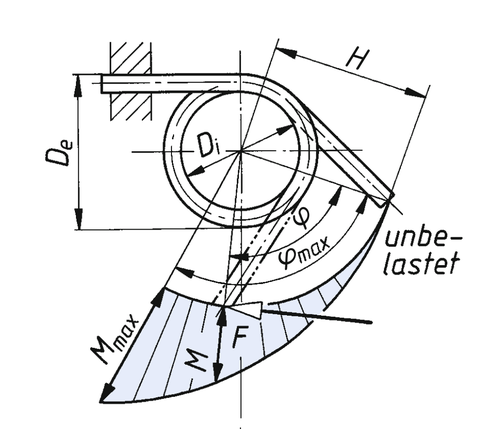
\includegraphics[width=0.4\linewidth,keepaspectratio]{graphics/drehfeder_kennwerte_moment_winkel.png}%
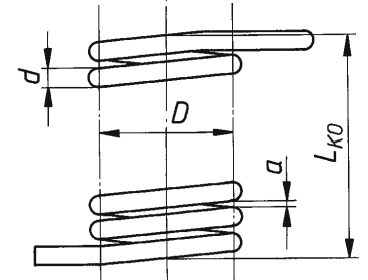
\includegraphics[width=0.35\linewidth,keepaspectratio]{graphics/drehfeder_abmessungen_drahtdurchmesser_federdurchmesser_lk0.png}
\end{figbox}

\begin{formulabox}
$\ZSFspringM = \ZSFspringR \cdot \ZSFspringPhi$

$\ZSFspringR = \dfrac{\pi}{180°}\cdot \dfrac{\ZSFspringE \cdot \ZSFspringD^4}{64 \cdot \ZSFspringDbig\cdot \ZSFspringNCoils}$
\formulanote{mit Normalkraft im Material $\ZSFspringE$}
$\ZSFspringW = \dfrac{\ZSFspringR \cdot (\ZSFspringPhiTwo^2 - \ZSFspringPhiOne^2)}{2} \text{, falls } \ZSFspringPhiOne = 0\text{; } \ZSFspringW = \dfrac{\ZSFspringMTwo \cdot \ZSFspringPhiTwo}{2}$
\end{formulabox}

\SubsubsectionBar{Drehstabfedern}
\ZSFindex{Drehstabfeder}

\begin{splitbox}[0.6]
\centering
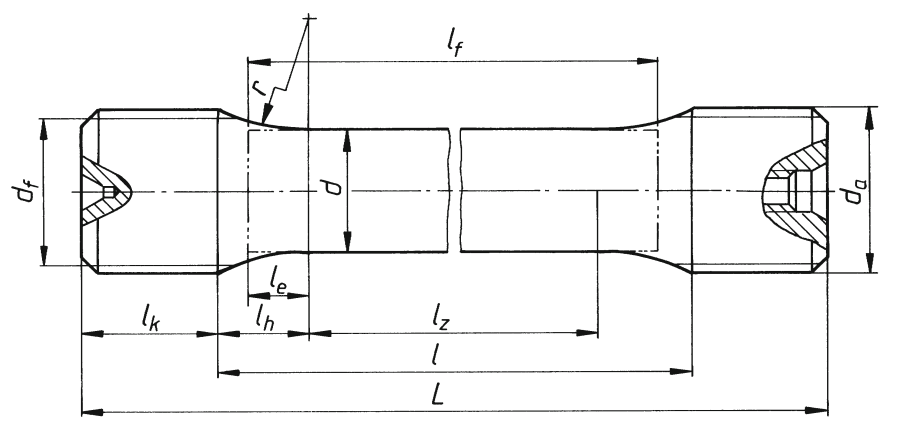
\includegraphics[width=\linewidth,keepaspectratio]{graphics/drehstabfeder_kennwerte_abmessungen.png}
\tcblower
{\centering $\displaystyle \ZSFspringR = \dfrac{\pi}{180°}\cdot \dfrac{\pi \cdot \ZSFspringG \cdot  \ZSFspringD^4}{32 \cdot \ZSFspringLf}$\par}
\ZSFgapXS
\formulanote{mit Torsion im Material $\ZSFspringG$}
\end{splitbox}

\SubsectionBarOnNewColumn[sec:biegefedern]{Biegefedern}
\ZSFindex{Biegefeder}
\ZSFindex{Blattfeder}

\ZSFfig[1.0]{graphics/v7_blattfeder_q1_werte.png}{}{}

\begin{formulabox}
$\ZSFspringR = \dfrac{\ZSFspringB \cdot \ZSFspringH^3 \cdot  \ZSFspringE}{\ZSFspringQOne \cdot \ZSFspringL^3}$
\end{formulabox}

\SubsubsectionBar{Zweiarmige Blattfedern}

\begin{splitbox}[0.45]
\centering
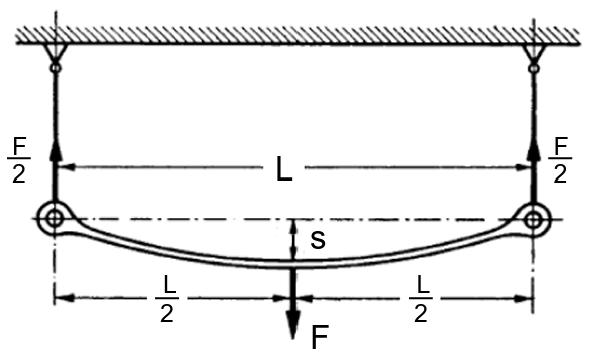
\includegraphics[width=\linewidth,keepaspectratio]{graphics/v7_zweiarmige_blattfeder_kennwerte.png}
\tcblower
$\approx$ Parallelschaltung von zwei einarmigen Blattfedern.

$\ZSFspringRers = \ZSFspringROne + \ZSFspringRTwo = 2\cdot \ZSFspringR$
\end{splitbox}

\begin{runintext}
Anwendung geschichteter Blattfedern: Federung von schweren Fahrzeugen wie Güterwagons, da zwischen den Federn starke Reibung auftritt, die dämpfend wirkt.
\end{runintext}

\SubsubsectionBar{Schnappverbindungen}
\ZSFindex{Schnappverbindung}

\begin{runintext}
Zwei einarmige Blattfedern mit Schnapphaken, die in einer Rastvorrichtung einschnappen können.
\end{runintext}

\ZSFfig[0.75]{graphics/v7_schnappverbindung_kennwerte.png}{}{}

\begin{factlist}
\item $\ZSFspringAlphaTwo < 90$° ist lösbar
\item $\ZSFspringAlphaTwo \geq 90$° nur mit einem Lösemechanismus lösbar
\end{factlist}

\begin{formulabox}
$\ZSFspringF = \ZSFspringR \cdot \ZSFspringS \qquad \ZSFspringR = \dfrac{\ZSFspringB \cdot \ZSFspringH^3 \cdot  \ZSFspringE}{4 \cdot \ZSFspringL^3}$
\end{formulabox}

% !TEX root = ../main.tex
% SECTION 6: LAGER, LAGERUNGEN UND SCHMIERUNG
% Inhalt: Liv Erne, Silvio Seiz — Form: ZSF-Template-Rework
% ============================================================

\StartChapter[ch:lager]{Lager, Lagerungen und Schmierung}

\SubsectionBar[sec:wälzlager]{Wälzlager}
\ZSFindex[walzlager]{Wälzlager}

\begin{defbox}[Wälzlager]
Bezeichnet das eigentliche mechanische Bauteil mit \ZSFkeyword{Innenring}, Käfig, Dichtung, \ZSFkeyword{Aussenring} und \ZSFkeyword[Walzkorper@Wälzkörper]{Wälzkörper}.
Verschiedene Formen mit unterschiedlichen Kontaktgeometrien, je nach Lastfall.
\end{defbox}

%\ZSFfig{graphics/rolling_bearing_deep_groove_radial_axial_load.png}{Wälzlager}{}
\begin{splitbox}[0.44]
  \begin{figbox}[Wälzlager-Bauformen]
    \centering
    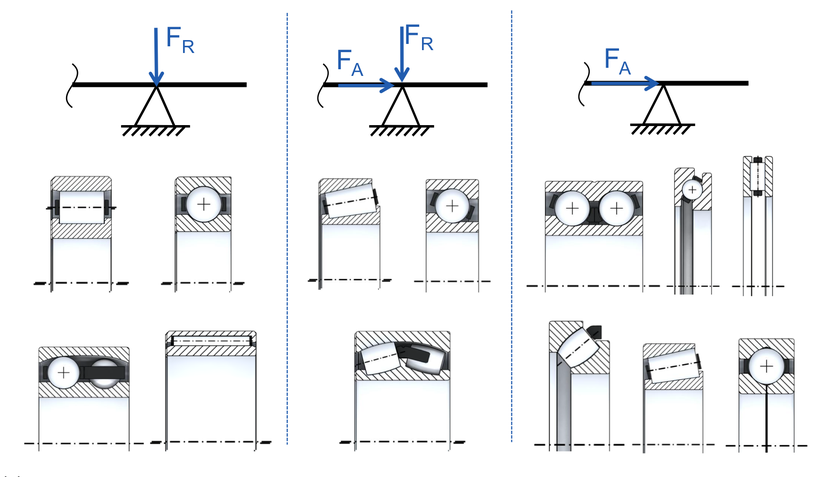
\includegraphics[width=\linewidth,keepaspectratio]{graphics/rolling_bearing_types_load_cases.png}% chktex 25
  \end{figbox}
\tcblower
  \begin{warnbox}[Lagerschäden]
    \begin{factlist}
    \item Wälzkörpereindrücke und Schlupfspuren bei falscher statischer Belastung.
    \item \ZSFkeyword{Pitting} und Fremdkörperüberrollung wenn Fremdstoffe in den Reibkontakt gelangen.
    \end{factlist}
  \end{warnbox}
\end{splitbox}
\ZSFindex[lagerschaden]{Lagerschäden}

\SubsectionBar[sec:lagerungen]{Lagerungen}
\ZSFindex{Lagerung}

\begin{tablebox}[Lagerungen: Definition, Funktion \& Bauarten]
  \ZSFReadableOn
  \setlength{\leftskip}{\ZSFspaceS}%
  \setlength{\rightskip}{\ZSFspaceS}%
  \vskip\ZSFspaceXS
  \textbf{Def:} Baugruppe, die ein Bauteil mit $\ge 2$ Lagern stützt/führt. \\
  \textbf{F1:} Rotation zulassen, Reibungsverluste reduzieren. \hfill
  \textbf{F2:} Freiheitsgrade begrenzen, Kräfte ableiten.
  \par
  \vskip\ZSFspaceXS
  \setlength{\leftskip}{0pt}%
  \setlength{\rightskip}{0pt}%
  \renewcommand{\arraystretch}{1.1}%
  \setlength{\tabcolsep}{2.0pt}%
  \begin{ZSFtable}[\ZSFfontTableDense]{Y{0.50} Y{1.30} Y{1.20}}
    \ZSFheaderRow 
    \ZSFhead{Lagerungen} & \ZSFhead{+} & \ZSFhead{--} \\
    \textbf{Fest-Los} & 
    $\cdot$ Wechselnde Axiallast \newline 
    $\cdot$ Eindeutige Position durch Festlager \newline 
    $\cdot$ Längenausgleich durch Loslager \newline 
    $\cdot$ Statisch bestimmt & 
    $\cdot$ Zusätzl. Bauteile \& Fertigungsschritte \\
    
    \textbf{Schwimmend} & 
    $\cdot$ Keine zusätzl. Bauteile oder Fertigungsschritte \newline 
    $\cdot$ Längenausgleich möglich & 
    $\cdot$ Axiales Spiel $\Rightarrow$ keine wechselnde Axiallast \newline 
    $\cdot$ Axiallast $\Rightarrow$ keine hohe Genauigkeit \\
    
    \textbf{Angestellt (X/O)} & 
    $\cdot$ Aufnahme hoher Axialkräfte \newline 
    $\cdot$ Hohe Positionsgenauigkeit \newline 
    $\cdot$ Gute Aufnahme von Kräften zw. Lagern & 
    $\cdot$ Sicherstellen der def. Vorspannung $\rightarrow$ hohe Kosten \newline 
    $\cdot$ Kein Längenausgleich $\rightarrow$ Schäden
  \end{ZSFtable}%
  
  \ZSFgapXS
  \setlength{\tabcolsep}{2.0pt}%
  \begin{ZSFtablePlain}[\ZSFfontTableDense]{Z{1.0} Z{1.0} Z{1.0} Z{1.0}}
    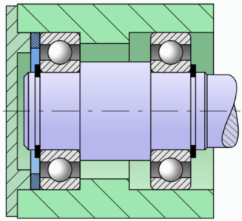
\includegraphics[width=0.95\hsize,height=1.45cm,keepaspectratio]{graphics/lagerung_fest_los.png} &
    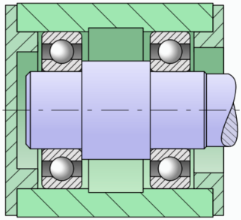
\includegraphics[width=0.95\hsize,height=1.45cm,keepaspectratio]{graphics/lagerung_schwimmend.png} &
    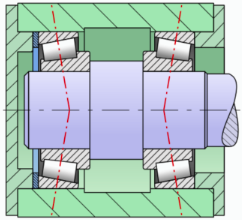
\includegraphics[width=0.95\hsize,height=1.45cm,keepaspectratio]{graphics/lagerung_angestellt_x.png} &
    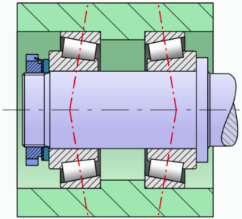
\includegraphics[width=0.95\hsize,height=1.45cm,keepaspectratio]{graphics/lagerung_angestellt_o.png} \\
    \TableTitle{Fest-Los} &
    \TableTitle{Schwimmend} &
    \TableTitle{Angestellt (X)} &
    \TableTitle{Angestellt (O)}
  \end{ZSFtablePlain}%
\end{tablebox}
\ZSFindex{Fest-Los-Lagerung}



\SubsubsectionBarOnNewColumn{Passungen / Punkt- und Umfangslast}
\ZSFindex{Punktlast}
\ZSFindex{Umfangslast}
\ZSFindex{Lebensdauer}

\begin{runintext}
Spiel-, Übergangs- und Presspassungen \ZSFref{sec:toleranzfeldbilder} beim Konstruieren von Wälzlagern zwischen Innenring und Welle, sowie Aussenring und Gehäude.
\end{runintext}

\ZSFfig[1.0]{graphics/rolling_bearing_point_circumferential_load_fit.png}{Punkt- und Umfangslast}{} % chktex 25

\begin{formulabox}[Lebensdauer und Tragfähigkeit]
\formulasources{$\ZSFbearP$:~\ZSFsource{bestimmen mit}{proc:lager-p}}
\[ \ZSFbearS = \dfrac{\ZSFbearR}{\ZSFbearB} \qquad \ZSFbearSZero = \dfrac{\ZSFbearCZero}{\ZSFbearPZero} \]
\[ \ZSFbearLTen = (\dfrac{\ZSFbearC}{\ZSFbearP})^\ZSFbearExp \qquad \ZSFbearLTenH = (\dfrac{\ZSFbearC}{\ZSFbearP})^\ZSFbearExp \cdot \dfrac{10^6}{60\cdot \ZSFbearN} \]
\[ \ZSFbearCerf = \ZSFbearP\cdot \sqrt[\ZSFbearExp]{\dfrac{60\cdot \ZSFbearN\cdot \ZSFbearLTenH}{10^6}} \]
\formulanote{$\ZSFbearLTen$:~nom. Lebensdauer \ $\cdot$ \ $\ZSFbearSZero$:~stat. Tragfähigkeit \ $\cdot$ \ $\ZSFbearCZero$:~stat. Tragzahl \\
$\ZSFbearPZero$:~stat. äquiv. Belastung \ $\cdot$ \ $\ZSFbearC$:~dyn. Tragzahl \ $\cdot$ \ $\ZSFbearP$:~dyn. äquiv. Tragzahl \\
$\ZSFbearExp$:~Lebensdauerexponent (Kugellager $\ZSFbearExp=3$, Rollenlager $\ZSFbearExp=10/3$)}
\end{formulabox}

\phantomsection\label{proc:lager-p}
\begin{procedure}[Dynamisch äquivalente Belastung $\ZSFbearP$ bestimmen]
\ProcStep{$\ZSFbearX$, $\ZSFbearY$, $\ZSFbearE$ bestimmen}{$\dfrac{\ZSFbearFZero\cdot \ZSFbearFa}{\ZSFbearCZero}\rightarrow Tabelle$ \ \ZSFmuted{$\dots\ZSFbearX, \ZSFbearY$ abhängig vom Lager}}
\ProcStep{Fallunterscheidung}{$\dfrac{\ZSFbearFa}{\ZSFbearFr} > \ZSFbearE \rightarrow \ZSFbearP = \ZSFbearX\cdot \ZSFbearFr + \ZSFbearY\cdot \ZSFbearFa$ \quad $\dfrac{\ZSFbearFa}{\ZSFbearFr} \leq \ZSFbearE \rightarrow \ZSFbearP = \ZSFbearFr$}
\end{procedure}

\SubsectionBar[sec:schmierung]{Schmierung}
\ZSFindex{Schmierung}

\begin{runintext}
\ZSFkeyword{Schmiermittel} wie Öle und Fette bilden auf den Oberflächen einen Film, der den direkten Kontakt von Stahl auf Stahl verhindert, um Reibung zu minimieren.
\end{runintext}

\begin{splitbox}[0.54]
  \begin{warnbox}[Beanspruchung \& Schädigung]
    \ZSFReadableOn
    \begin{factlist}
      \item \ZSFkeyword{Hertzsche Pressung}:~Höchste Beanspruchung knapp \ZSFhl{unter der Oberfläche} $\rightarrow$ Risskeime, \ZSFkeyword{Pitting} (Grübchen).
      \item \textbf{Verschleiss}:~Abrieb durch Schmutz/Mangelschmierung.
      \item \textbf{Korrosion}:~Rost/Stromdurchgang schädigt Laufbahnen.
    \end{factlist}
  \end{warnbox}
\tcblower
  \begin{figbox}[Stribeck-Kurve]
    \centering
    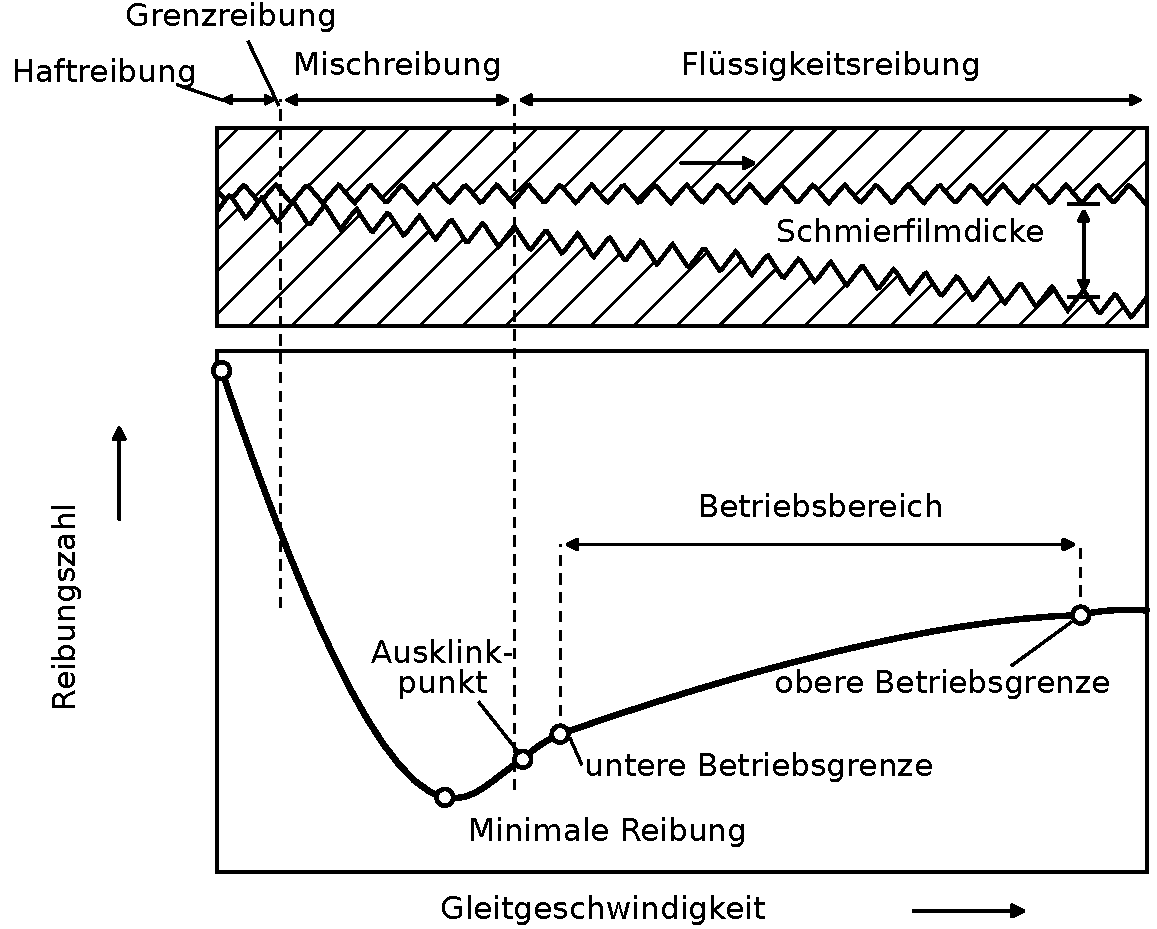
\includegraphics[width=0.98\linewidth,keepaspectratio]{graphics/stribeck.pdf}
  \end{figbox}
\end{splitbox}
\ZSFindex{Stribeck-Kurve}

% !TEX root = ../main.tex
% SECTION 7: KUPPLUNGEN
% Inhalt: Liv Erne, Silvio Seiz — Form: ZSF-Template-Rework
% ============================================================

\StartChapter[ch:kupplungen]{Kupplungen}
\ZSFindex{Kupplung}

\ZSFfig[0.70]{graphics/v9_kupplungsbaum_entscheidungsbaum.png}{Kupplungsbaum}{}\begin{propertylist}[Eigenschaften]
\ZSFFact{Schaltbar}{Verbindung/Trennung des Drehmomentflusses}
\ZSFFact{Drehsteif}{Drehmomentstösse/Schwankungen gehen ungefiltert durch}
\ZSFFact{Drehelastisch}{Dämpfung von Stössen/Schwankungen (Gummi, Federn)}
\ZSFFact{Ausgleichend}{Ausgleich von Versatz:~axial ($\ZSFcoupDeltaKa$), radial ($\ZSFcoupDeltaKr$), winklig ($\ZSFcoupDeltaKw$)}
\ZSFFact{Fremdbetätigt}{Betätigung von aussen (manuell, hydr., el.)}
\ZSFFact{Selbstbetätigt}{Schaltet selbsttätig bei Grenzwert:\\
-- \textbf{Drehzahl}:~Schalten ab $\ZSFcoupNlimit$ (Fliehkraftkupplung)\\
-- \textbf{Moment}:~Rutschen bei Überlast $\ZSFcoupMlimit$ (Sicherheitsk.)\\
-- \textbf{Richtung}:~Freilauf / Sperrrichtung (Freilaufkupplung)}
\end{propertylist}

\SubsectionBarOnNewColumn[sec:fliehkraftkupplung]{Fliehkraftkupplung (drehzahlbetätigt)}
\ZSFindex{Fliehkraftkupplung}

\begin{splitbox}[0.45]
Durch die Drehbewegung werden die \ZSFkeyword[Fliehgewicht]{Fliehgewichte} im Inneren der Kupplung nach aussen gedrückt, wodurch ein Reibschluss mit der Kupplungsglocke entsteht. Die Berechnungen weichen, je nach Anzahl Fliehgewichte, ab: Gleichgewicht zwischen Federkraft $\ZSFcoupFF = \ZSFcoupFV$ und $\ZSFcoupFz$ aufstellen.
\tcblower
\centering
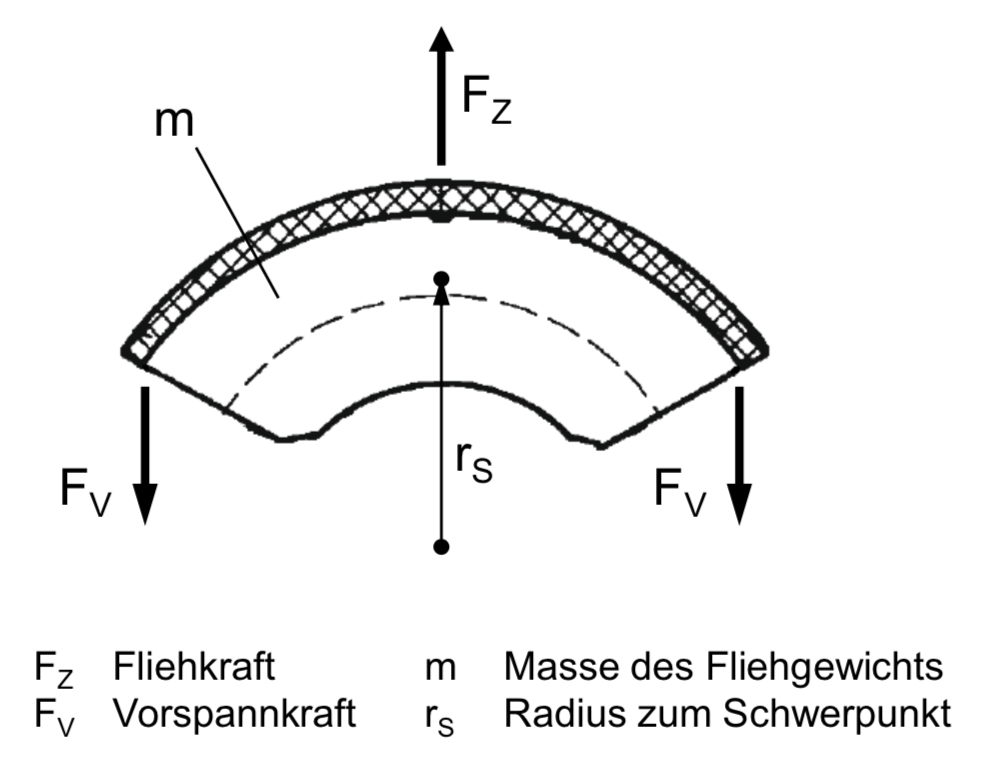
\includegraphics[width=\linewidth,keepaspectratio]{graphics/centrifugal_clutch_weight_forces.png}
\end{splitbox}
% Danger-Pill unbrechbar (~190pt) — passt nur in voller Spaltenbreite,
% deshalb direkt nach der splitbox statt in deren schmaler Textspalte.
\ZSFdanger{so kann es bei den Drehzahl Formeln auch sin oder cos drin haben}

\begin{formulabox}[Drehzahlen]
\formulasources{$\ZSFcoupFV$, $\ZSFcoupR$:~gegeben oder \ZSFsource{bestimmen mit}{sec:zugdruckfedern}}
\[ \ZSFcoupFz = \ZSFcoupNf\cdot \ZSFcoupFV = \dfrac {\ZSFcoupMass\cdot \ZSFcoupV^2}{\ZSFcoupRs} = \ZSFcoupMass\cdot \ZSFcoupRs \cdot (2\cdot \pi \cdot \ZSFcoupN)^2 = \dfrac{\ZSFcoupMass\cdot \ZSFcoupRs \cdot 4\cdot \pi^2}{\ZSFcoupT^2} \]
\[ \ZSFcoupNG^2 = \dfrac{\ZSFcoupNf\cdot \ZSFcoupFV}{\ZSFcoupMass\cdot \ZSFcoupRs \cdot 4\cdot \pi^2} \quad \text{\textbf{Grenzdrehzahl}} \]
\formulasep
\[ \ZSFcoupNE^2 = \dfrac{\ZSFcoupNf\cdot (\ZSFcoupFV + \ZSFcoupR\cdot \ZSFcoupApos)}{\ZSFcoupMass\cdot (\ZSFcoupRs + \ZSFcoupApos) \cdot 4\cdot \pi^2} \quad \text{\textbf{Einschaltdrehzahl}} \]
\[ \ZSFcoupNB^2 = \dfrac{\ZSFcoupFN + \ZSFcoupNf\cdot (\ZSFcoupFV + \ZSFcoupR\cdot \ZSFcoupApos)}{\ZSFcoupMass\cdot (\ZSFcoupRs + \ZSFcoupApos) \cdot 4\cdot \pi^2} \quad \text{\textbf{Betriebsdrehzahl}} \]
\formulanote{$\ZSFcoupN^2 = [s^{-2}]$, $\ZSFcoupN = [s^{-1}]\rightarrow\cdot 60 = \ZSFcoupN = [min^{-1}]$}
\[ \ZSFcoupFN = \dfrac{\ZSFcoupM}{\ZSFcoupZ\cdot \ZSFcoupMu \cdot \ZSFcoupRk} \]
\formulanote{$\ZSFcoupZ$:~Anzahl Fliehgewichte \ $\cdot$ \ $\ZSFcoupRk$:~wirksamer Reibradius}
\formulanote{$\ZSFcoupNf$:~Anzahl Federn pro Fliehgewicht \ $\cdot$ \ $\ZSFcoupR$:~Federrate}
\formulanote{\ZSFdanger{Achtung:} $2\cdot \ZSFcoupR\cdot \ZSFcoupApos$, anstelle $\ZSFcoupR\cdot \ZSFcoupApos$, falls der Weg a zweimal gemacht wird.}
\end{formulabox}
\ZSFindex{Grenzdrehzahl}
\ZSFindex{Einschaltdrehzahl}
\ZSFindex{Betriebsdrehzahl}

\SubsectionBar[sec:rutschkupplung]{Rutsch- o. Sicherheitskupplung (momentbetätigt)}
\ZSFindex{Rutschkupplung}
\ZSFindex{Sicherheitskupplung}

\begin{splitbox}[0.57]
\centering
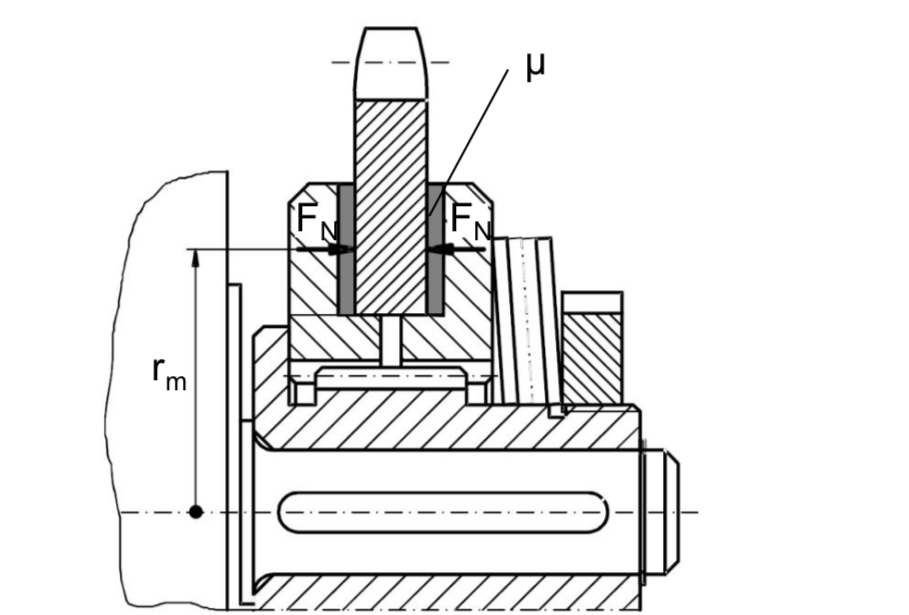
\includegraphics[width=\linewidth,keepaspectratio]{graphics/rutschkupplung_reibscheiben_normalkraft_reibwert.png}
\tcblower
\centering
$\begin{aligned}
\ZSFcoupFt &= \ZSFcoupZR\cdot \ZSFcoupFr \\[1pt]
\ZSFcoupFr &= \ZSFcoupMu \cdot \ZSFcoupFN \\[1pt]
\ZSFcoupRm &= \dfrac{\ZSFcoupDa + \ZSFcoupDi}{4} \\[1pt]
\ZSFcoupP &= \dfrac{\ZSFcoupFN}{\ZSFcoupAm} \\[1pt]
\ZSFcoupAm &= \dfrac{\pi}{4}\cdot (\ZSFcoupDa^2 - \ZSFcoupDi^2) \\[1pt]
\ZSFcoupFN &= \ZSFcoupNFedern \cdot \ZSFcoupFV
\end{aligned}$

\ZSFgapXS
{\ZSFfontNote $\ZSFcoupFV$:~Vorspannkraft einer Feder \ $\cdot$ \ $\ZSFcoupZR$:~Anzahl Reibflächen \\
$\ZSFcoupDa$:~Aussendurchmesser \ $\cdot$ \ $\ZSFcoupDi$:~Innendurchmesser\par}
\end{splitbox}

\begin{formulabox}[Grenzmoment $\ZSFcoupMG$]
\[ \ZSFcoupMG = \ZSFcoupFt \cdot \ZSFcoupRm = \ZSFcoupZR\cdot \ZSFcoupMuG \cdot \ZSFcoupFN \cdot \ZSFcoupRm \]
\formulanote{$\ZSFcoupMuG$:~Gleitreibwert \ $\cdot$ \ $\ZSFcoupZR$:~Anzahl Flächen oder Reibkontakte}
\end{formulabox}

\SubsectionBar[sec:nichtschaltbar]{Nicht schaltbare Kupplungen}
\ZSFindex{Kupplung!nicht schaltbar}

\begin{tablebox}[Nicht schaltbare Kupplungen: Drehsteif]
\ZSFKupplungenDrehsteifTabelle
\end{tablebox}

\begin{tablebox}[Nicht schaltbare Kupplungen: Drehelastisch]
\ZSFKupplungenDrehelastischTabelle
\end{tablebox}

\begin{tablebox}[Grosser Radialversatz / Winkelausgleich]
\setlength{\tabcolsep}{2.0pt}
\begin{ZSFtablePlain}[\ZSFfontTableDense]{Z{1.0} Z{1.0} Z{1.0}}
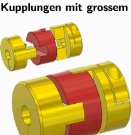
\includegraphics[height=0.7cm,keepaspectratio]{graphics/kreuzscheibenkupplung.png} &
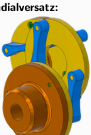
\includegraphics[height=0.7cm,keepaspectratio]{graphics/parallelkurbelkupplung.png} &
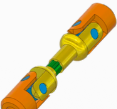
\includegraphics[height=0.7cm,keepaspectratio]{graphics/kardangelenkwelle.png} \\
\TableTitle{Kreuzscheiben\-kupplung} &
\TableTitle{Parallelkurbel\-kupplung} &
\TableTitle{Kardangelenkwelle}
\end{ZSFtablePlain}
\end{tablebox}

% !TEX root = ../main.tex
% SECTION 8: SCHRAUBEN
% Inhalt: Liv Erne, Silvio Seiz — Form: ZSF-Template-Rework
% ============================================================

\StartChapter[ch:schrauben]{Schrauben}
\ZSFindex{Schraube}

\begin{runintext}
Mit Schraubenmutter, Innengewinde, Schraubenkopf, Schraubenschaft und Aussengewinde.
\end{runintext}

\begin{formulabox}
\ZSFkeyword*{Eindrehwinkel und Weg}:~$\ZSFscrewAlpha = \dfrac{\ZSFscrewS}{\ZSFscrewP}\cdot 360° \qquad \ZSFscrewS = \dfrac{\ZSFscrewAlpha}{360°}\cdot \ZSFscrewP$
\formulanote{$\ZSFscrewAlpha =$ Eindrehwinkel, $\ZSFscrewS =$ Weg, $\ZSFscrewP =$ Steigung}
\end{formulabox}

\begin{tablebox}[Schraubenköpfe]
\renewcommand{\arraystretch}{1.3}
\begin{ZSFtable}[\ZSFfontTableDense]{Z{0.75} Z{1.25} Z{1.125} Z{0.75} Z{1.125}}
\ZSFheaderRow \ZSFhead{Kopf} & \ZSFhead{Name} & \ZSFhead{Anzieh\-moment} & \ZSFhead{Preis} & \ZSFhead{Montage} \\

\includegraphics[width=0.65\hsize,keepaspectratio]{graphics/v10_slotted_screw_drive.png} & Längsschlitz & niedrig & günstig & schlechte Zentrierung \\

\includegraphics[width=0.65\hsize,keepaspectratio]{graphics/v10_schraubenantrieb_kreuzschlitz.png} & Kreuzschlitz & niedrig & günstig & gute Zentrierung \\

\includegraphics[width=0.65\hsize,keepaspectratio]{graphics/v10_schraubenkopf_aussensechskant.png} & Aussensechskant & hoch & günstig & grosser Platzbedarf \\

\includegraphics[width=0.65\hsize,keepaspectratio]{graphics/v10_schraubenantrieb_innensechskant.png} & Innensechskant (Imbus) & mittel & günstig & wenig Platzbedarf \\

\includegraphics[width=0.65\hsize,keepaspectratio]{graphics/v10_schraubenkopf_aussenvielzahn.png} & Aussenvielzahn & sehr hoch & teuer & grosser Platzbedarf \\

\includegraphics[width=0.65\hsize,keepaspectratio]{graphics/v10_schraubenantrieb_innenvielzahn_torx.png} & Innenvielzahn (Torx) & hoch & teuer & wenig Platzbedarf
\end{ZSFtable}
\end{tablebox}
\ZSFindex[schraubenkopfe]{Schraubenköpfe}

\SubsectionBar[sec:gewinde]{Gewinde}
\ZSFindex{Gewinde}

\begin{runintext}
Wandelt Rotation in Translation. Links- und Rechtsgewinde (Standard).
\end{runintext}

\begin{valuegrid}{1}[Gewindearten]
Metrisch & $\ZSFscrewBeta = 60^\circ$ \\
Whitworth & $\ZSFscrewBeta = 55^\circ$ \\
Trapez & $\ZSFscrewBeta = 30^\circ$ \\
Sägen & $\ZSFscrewBeta = 30^\circ$ resp. $3^\circ$
\end{valuegrid}

\begin{valuegridtwo}[Metrisches Gewinde (Beispiele)]
Regelgewinde & M10 & $\ZSFscrewD = 10\,\text{mm}, \ZSFscrewP = 1.5\,\text{mm}$ \\
Feingewinde & $M10\times 1.25$ & $\ZSFscrewD = 10\,\text{mm}, \ZSFscrewP = 1.25\,\text{mm}$
\end{valuegridtwo}
\ZSFindex{Feingewinde}
\ZSFindex{Gewinde, metrisches}

\begin{formulabox}[Gewindeprofil (ISO)]
\[ \ZSFscrewH = \dfrac{\sqrt{3}}{2}\cdot \ZSFscrewP \qquad \ZSFscrewHThree = \ZSFscrewH - \dfrac{\ZSFscrewH}{6}- \dfrac{\ZSFscrewH}{8} \]
\formulanote{$\ZSFscrewH$:~Profilhöhe \ $\cdot$ \ $\ZSFscrewHThree$:~Gewindetiefe \ $\cdot$ \ $\ZSFscrewP$:~Steigung}
\end{formulabox}

\begin{figbox}[Gewindegeometrie]
\begin{minipage}[c]{0.54\linewidth}\centering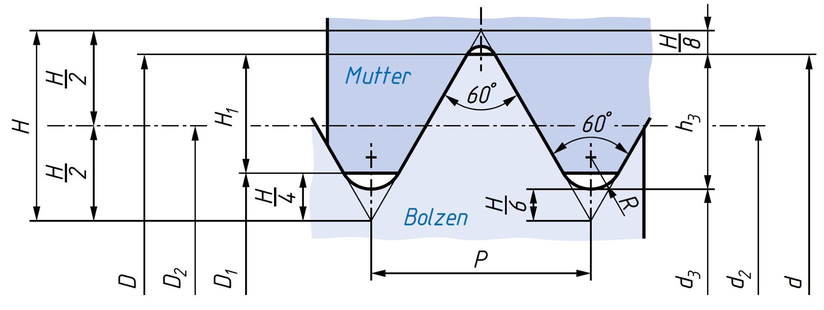
\includegraphics[width=\linewidth,keepaspectratio]{graphics/v10_schrauben_metrisches_iso_gewinde.png}\end{minipage}\hfill\begin{minipage}[c]{0.42\linewidth}\centering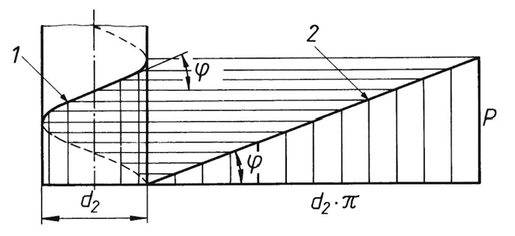
\includegraphics[width=\linewidth,keepaspectratio]{graphics/v10_schrauben_gewinde_kennwerte.png}\end{minipage}
\end{figbox}

\ZSFfig[0.85]{graphics/v10_schraubenquerschnitte.png}{}{}

\begin{formulabox}[Steigungswinkel \& Querschnitte]
\[ \tan \ZSFscrewPhi = \dfrac{\ZSFscrewP}{\ZSFscrewDTwo \cdot \pi} \qquad \ZSFscrewDs = \dfrac{1}{2} \cdot (\ZSFscrewDTwo + \ZSFscrewDThree) \]
\formulanote{$\ZSFscrewPhi$:~Steigungswinkel \ $\cdot$ \ $\ZSFscrewDTwo$:~Flankend. \ $\cdot$ \ $\ZSFscrewDThree$:~Kernd. \ $\cdot$ \ $\ZSFscrewDs$:~Spannungsd. \ $\cdot$ \ $\ZSFscrewA = \ZSFscrewAN$:~Nennquerschn. \ $\cdot$ \ $\ZSFscrewAk = \ZSFscrewAThree$:~Kernquerschn.}
\end{formulabox}

\SubsectionBar[sec:festigkeitsklassen]{Festigkeitsklassen}
\ZSFindex{Festigkeitsklasse}

\begin{figbox}
\centering
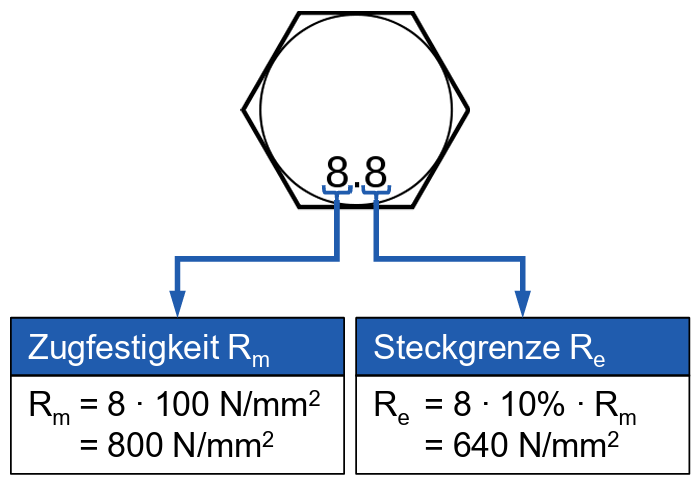
\includegraphics[width=0.38\linewidth,keepaspectratio]{graphics/v10_schraube_festigkeitsklasse_beispiel_8_8.png}%
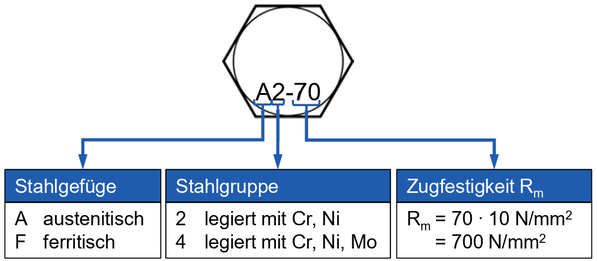
\includegraphics[width=0.58\linewidth,keepaspectratio]{graphics/v10_schraube_festigkeitsklassen_tabelle.png}
\end{figbox}

\SubsectionBar[sec:schraubenverbindungen]{Schraubenverbindungen}
\ZSFindex{Schraubenverbindung}

\begin{runintext}
Weil die Schraube beim Festziehen wie eine Feder auf Zug belastet wird, werden zwei Bauteile kraftschlüssig aufeinandergepresst, wodurch die Verbindung durch \ZSFkeyword*{Reibschluss} hält. Der Lastanteil nimmt pro Windung der Schraube immer mehr ab.
\end{runintext}

\begin{figbox}
  \noindent
  \begin{minipage}[c]{0.46\linewidth}%
    \centering
    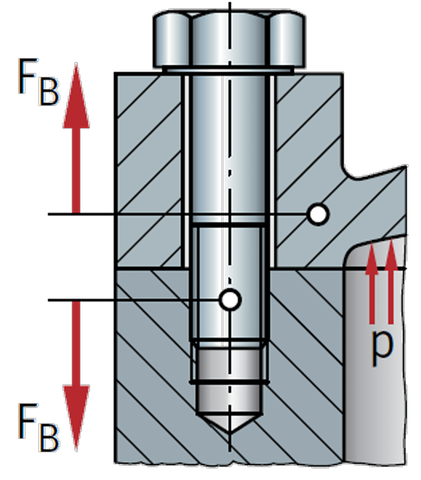
\includegraphics[width=0.48\linewidth,keepaspectratio]{graphics/v10_schraubenverbindung_einschraubverbindung.png}\hfill
    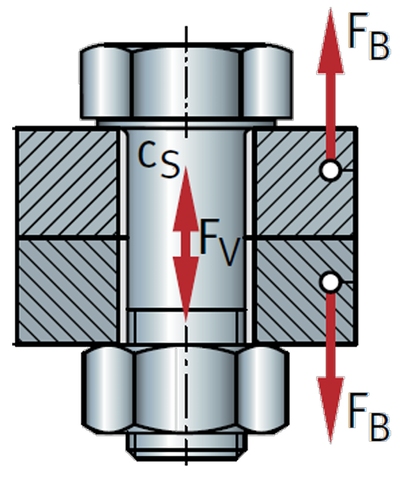
\includegraphics[width=0.48\linewidth,keepaspectratio]{graphics/v10_schraubenverbindung_durchsteckverbindung.png}%
  \end{minipage}%
  \hfill
  \begin{minipage}[c]{0.50\linewidth}%
    \raggedright
    \ZSFReadableOn
    \textbf{Gestaltungsfehler}:
    \begin{factlist}
    \item Kein Platz für Schraubenkopf
    \item Zu wenig Plattenmaterial
    \item Kein Spiel zwischen Schraubenkopf und Platten
    \item Unebene Auflagefläche für Schraubenkopf und -Mutter
    \end{factlist}
  \end{minipage}%
  \par
\end{figbox}
\ZSFindex{Einschraubverbindung}
\ZSFindex{Durchsteckverbindung}
\ZSFindex{Gestaltungsfehler}

\SubsectionBar[sec:schraubenbelastung]{Belastung der Schraube}
\ZSFindex{Anziehdrehmoment}

\begin{runintext}
Beim Anziehen entsteht ein zwei-achsiger Spannungszustand: \ZSFkeyword{Zugspannung} ($\ZSFscrewSigmaZ$) durch die Vorspannkraft $\ZSFscrewFv$ und \ZSFkeyword{Torsionsspannung} ($\ZSFscrewTauT$) durch Verdrehen gegen Gewindesteigung ($\ZSFscrewPhi$), Flanken- ($\ZSFscrewRhoPrime$) und Kopfreibung ($\ZSFscrewMuk$) beim Anziehdrehmoment $\ZSFscrewMA$.
\end{runintext}

\begin{formulabox}
\formulasources{Kräfte:~\ZSFsource{aus}{sec:verspannungsschaubild} \ $\cdot$ \ Gewindegrössen:~\ZSFsource{aus}{sec:gewinde} \ $\cdot$ \ $\ZSFscrewWtThree$:~\ZSFsource{bestimmen mit}{sec:widerstandsmoment}}
\ZSFkeyword*{Spannungen beim Anziehen}:~$\ZSFscrewSigmaZ = \frac{\ZSFscrewFsMax}{\ZSFscrewAs} \qquad \ZSFscrewTauT = \dfrac {\ZSFscrewMGMax}{\ZSFscrewWtThree}$

$\ZSFscrewMGMax = \tan(\ZSFscrewPhi + \ZSFscrewRhoPrime) \cdot \dfrac{\ZSFscrewFvMax \cdot \ZSFscrewDTwo}{2} \qquad \tan \ZSFscrewRhoPrime = \dfrac{\ZSFscrewMuG}{\cos(\ZSFscrewBeta/2)}$
\formulanote{$\ZSFscrewRhoPrime$:~Reibungswinkel \ $\cdot$ \ $\ZSFscrewFvMax$:~maximale Montagevorspannkraft (Axialkraft der Schraube) \ $\cdot$ \ $\ZSFscrewMG$:~Gewindemoment \ $\cdot$ \ $\ZSFscrewWtThree$:~Torsionswiderstandsmoment bei $\ZSFscrewDThree$}
\end{formulabox}

\begin{figbox}
\noindent
\begin{minipage}[c]{0.52\linewidth}
  \raggedright
  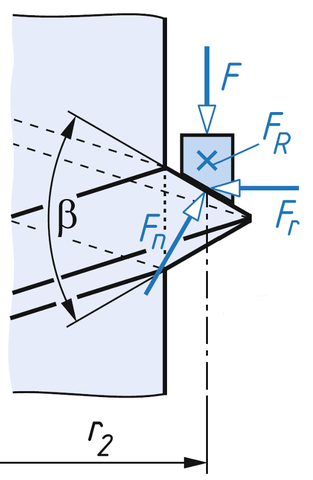
\includegraphics[width=0.48\linewidth,keepaspectratio]{graphics/v10_schraube_modell_spitzgewinde.png}\hfill
  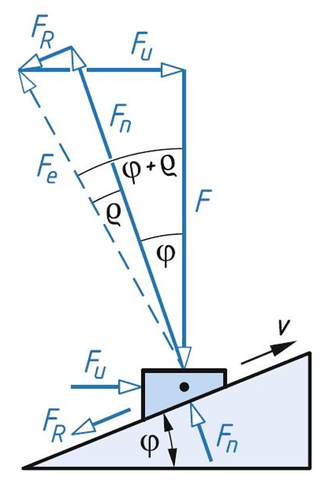
\includegraphics[width=0.48\linewidth,keepaspectratio]{graphics/v10_schraube_modell_reibung_steigung.png}
\end{minipage}\hfill
\begin{minipage}[c]{0.44\linewidth}
  \centering
  $\displaystyle \ZSFscrewFu = \ZSFscrewFv\cdot\tan(\ZSFscrewPhi + \ZSFscrewRhoPrime)$
  \par\ZSFgapS
  {\ZSFfontNote In der Grafik gilt: $\ZSFscrewF = \ZSFscrewFv$.\par}
\end{minipage}
\end{figbox}

\begin{formulabox}
\formulasources{Gewindegrössen:~\ZSFsource{aus}{sec:gewinde} \ $\cdot$ \ $\ZSFscrewFvMax$:~\ZSFsource{aus}{sec:verspannungsschaubild}}
\ZSFkeyword*{Modell: Reibung und Steigung}: $\ZSFscrewFu = \ZSFscrewF\cdot \tan(\ZSFscrewPhi + \ZSFscrewRho) \qquad \ZSFscrewMG = \dfrac{\ZSFscrewDTwo \cdot \ZSFscrewFu}{2} \qquad \ZSFscrewMu = \tan \ZSFscrewRho$

$\ZSFscrewFn = \dfrac{\ZSFscrewF}{cos(\ZSFscrewBeta/2)} \qquad \tan \ZSFscrewPhi = \dfrac{\ZSFscrewFu}{\ZSFscrewF}$
\formulanote{$\dots$ohne Reibung}
$\ZSFscrewFr = \ZSFscrewMu \cdot \ZSFscrewFn = \tan \ZSFscrewRho \cdot \ZSFscrewFn$
\formulanote{$\dots$mit Reibung}
\formulasep
\ZSFkeyword*{Anziehdrehmoment $\ZSFscrewMA$}: $\ZSFscrewMA = \ZSFscrewFvMax \cdot (\dfrac{\ZSFscrewDTwo}{2}\cdot \tan(\ZSFscrewPhi + \ZSFscrewRhoPrime) + \ZSFscrewMuk \cdot \dfrac{\ZSFscrewDk}{2}) \approx 0,17 \cdot \ZSFscrewFvMax \cdot \ZSFscrewD$
\formulanote{$\dots$Anziehdrehmoment mit Kopfreibung $\ZSFscrewMuk$ und maximaler Montagevorspannkraft $\ZSFscrewFvMax$. Bei Sechskant- und Zylinderschrauben, mit metrischem Gewinde ist $\ZSFscrewMuk = 0.12$ und $\dfrac{\ZSFscrewDk}{2} = 0.65\cdot \ZSFscrewD$.}
\end{formulabox}

\SubsectionBar[sec:verspannungsschaubild]{Verspannungsschaubild / Nachgiebigkeit}
\ZSFindex{Verspannungsschaubild}
\ZSFindex{Nachgiebigkeit}
\ZSFindex{Setzkraftverlust}

\begin{runintext}
Durch die \ZSFkeyword{Vorspannkraft} $\ZSFscrewFv$ der Schraube werden die Platten gestaucht ($\ZSFscrewFt$) und die Schrauben verlängert ($\ZSFscrewFs$), wobei $\ZSFscrewDeltaST$ die \ZSFkeyword*{Nachgiebigkeit} der Schraube/ verspannten Teile ist. Ebenfalls führt sie in den hochbelasteten Oberflächen zu plastischen Verformungen (\ZSFkeyword{Setzen}), also zur Abnahme der Vorspannkraft $\rightarrow$ \ZSFkeyword*{Setzkraftverlust} $\ZSFscrewFz$
\end{runintext}

\phantomsection\label{formula:screw-compliances}
\begin{formulabox}[Nachgiebigkeiten $\ZSFscrewDelta$]
\formulasources{Lage der $\ZSFscrewDeltai$:~\ZSFsource{aus}{sec:nachgiebigkeiten-orte}}
\[ \ZSFscrewF = \dfrac{\ZSFscrewFSmall}{\ZSFscrewDelta} \qquad \ZSFscrewDelta = \dfrac{\ZSFscrewL}{\ZSFscrewE\cdot \ZSFscrewA} \qquad \ZSFscrewR = \dfrac{\ZSFscrewE \cdot \ZSFscrewA}{\ZSFscrewL} \qquad \ZSFscrewFsT = \ZSFscrewDeltaST \cdot \ZSFscrewFv \]
\[ \ZSFscrewDeltaS = \ZSFscrewDeltaKo + \ZSFscrewDeltaOne + \ZSFscrewDeltaTwo + \ZSFscrewDeltaG + \ZSFscrewDeltaGe + \ZSFscrewDeltaM =\sum\ZSFscrewDeltai \]
\[ \ZSFscrewDeltaS = \frac{1}{\ZSFscrewES}\cdot\left(\frac{\ZSFscrewLKo}{\ZSFscrewAN}+\frac{\ZSFscrewLOne}{\ZSFscrewAdOne}+\frac{\ZSFscrewLTwo}{\ZSFscrewAdTwo}+\frac{\ZSFscrewLG}{\ZSFscrewAThree}+\frac{\ZSFscrewLGe}{\ZSFscrewAThree}\right)+\frac{\ZSFscrewLM}{\ZSFscrewEM\cdot \ZSFscrewAN} \]
\[ \ZSFscrewAN = \dfrac{\pi}{4}\cdot \ZSFscrewD^2 \qquad \ZSFscrewDeltaT = \dfrac{\ZSFscrewLk}{\ZSFscrewET \cdot \ZSFscrewAers} \]
\[ \ZSFscrewAers = \frac{\pi}{4}\cdot(\ZSFscrewDw^2 -\ZSFscrewDh^2) + \frac{\pi}{8}\cdot \ZSFscrewDw \cdot(\ZSFscrewDA - \ZSFscrewDw) \cdot ((\ZSFscrewX+1)^2-1) \]
\[ \ZSFscrewX = \sqrt[3]{\frac{\ZSFscrewLk\cdot \ZSFscrewDw}{\ZSFscrewDA^2}} \qquad \ZSFscrewDA \leq \ZSFscrewDw + \ZSFscrewLk \]
\end{formulabox}

\begin{figbox}[Nachgiebigkeit (Geometrie)]
\centering
\raisebox{\depth}{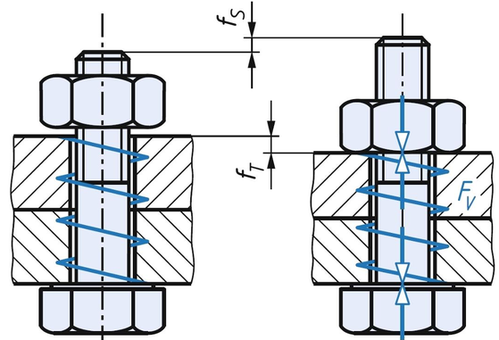
\includegraphics[width=0.33\linewidth,angle=-90,keepaspectratio]{graphics/v10_schraube_verspannungsschaubild.png}}%
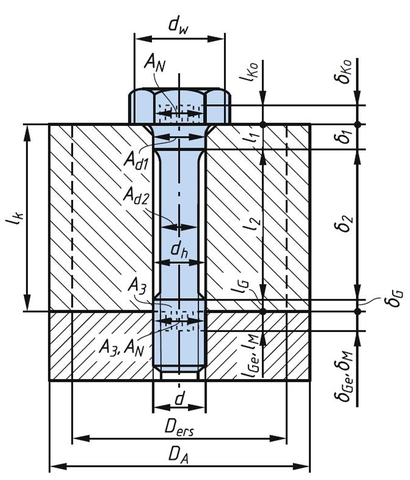
\includegraphics[width=0.36\linewidth,keepaspectratio]{graphics/v10_nachgiebigkeit_schraube.png}%
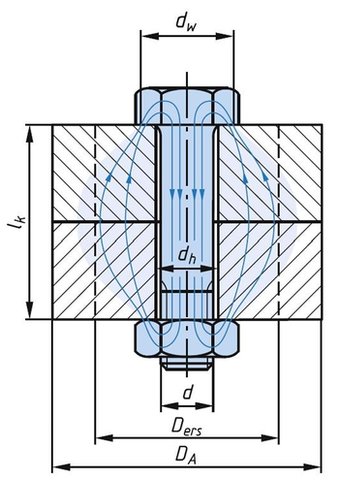
\includegraphics[width=0.30\linewidth,keepaspectratio]{graphics/v10_nachgiebigkeit_verspannte_teile.png}
\end{figbox}

\begin{formulabox}[Betriebs- und Vorspannkräfte]
\formulasources{$\ZSFscrewDeltaS$, $\ZSFscrewDeltaT$:~\ZSFsource{aus}{formula:screw-compliances} \ $\cdot$ \ $\ZSFscrewKA$:~\ZSFsource{aus}{sec:anziehwert}}
\[ \ZSFscrewFB = \ZSFscrewFBS + \ZSFscrewFBT \qquad \ZSFscrewFBS = \dfrac{\ZSFscrewDeltaT \cdot \ZSFscrewFB}{\ZSFscrewDeltaS + \ZSFscrewDeltaT} \qquad \ZSFscrewFBT = \dfrac{\ZSFscrewDeltaS \cdot \ZSFscrewFB}{\ZSFscrewDeltaS + \ZSFscrewDeltaT} \]
\[ \ZSFscrewFz = \dfrac{\ZSFscrewFSmallZ}{\ZSFscrewDeltaS + \ZSFscrewDeltaT} \qquad \ZSFscrewFsMax = \ZSFscrewFvMax + \ZSFscrewFBS \]
\[ \ZSFscrewFvMin = \ZSFscrewFkl + \ZSFscrewFz + \ZSFscrewFBT \qquad \ZSFscrewFvMax = \ZSFscrewKA \cdot \ZSFscrewFvMin \]
\formulanote{$\ZSFscrewFz =$ Setzkraftverlust, $\ZSFscrewFkl =$ Klemmkraft, $\ZSFscrewKA =$ Anziehfaktor, $\ZSFscrewFvMax =$ maximale Montagevorspannkraft, $\ZSFscrewFS =$ Schraubenkraft}
\end{formulabox}
\ZSFindex{Klemmkraft}
\ZSFindex{Montagevorspannkraft}

\begin{figbox}[Verspannungsschaubilder]
\centering
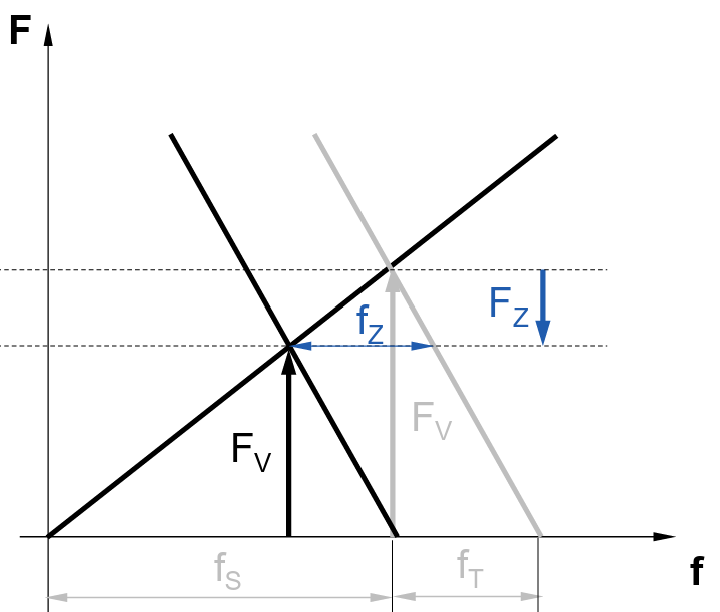
\includegraphics[width=0.22\linewidth,keepaspectratio]{graphics/v10_schraube_setzkraftverlust_diagramm.png}%
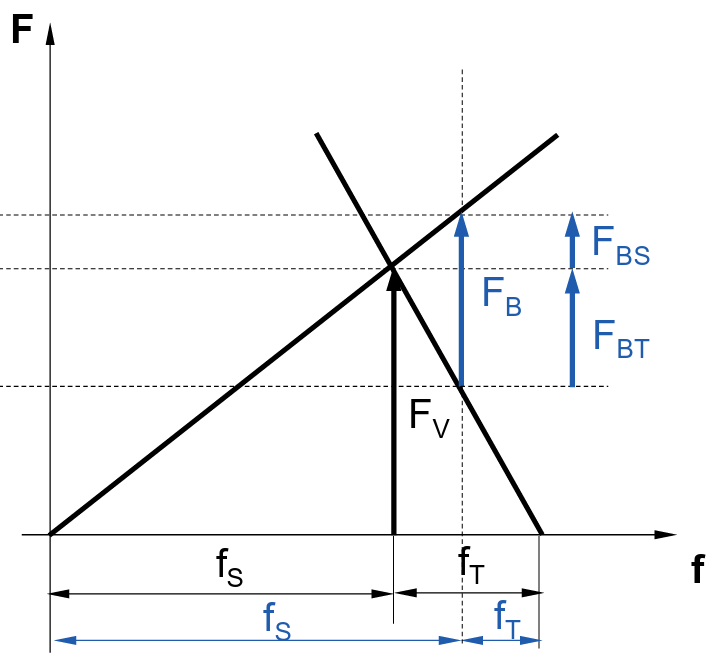
\includegraphics[width=0.22\linewidth,keepaspectratio]{graphics/v10_bolt_force_components_diagram.png}
\end{figbox}

% !TEX root = ../main.tex
% SECTION 9: MECHANISCHE MECHANISMEN
% Inhalt: Liv Erne, Silvio Seiz — Form: ZSF-Template-Rework
% ============================================================

\StartChapter[ch:mechanismen]{Mechanische Mechanismen}
\ZSFindex{Mechanismus}

\begin{runintext}
Kopplung von Elementen, bei der jede Bewegung eine andere bewirkt: Kraftverstärkung, Rotation zu Translation
\end{runintext}

\SubsectionBar[sec:force-amplification]{Kraftverstärkung}
\ZSFindex[kraftverstarkung]{Kraftverstärkung}

\begin{runintext}
$\rightarrow$ Weniger Kraft, mehr Weg: $W_1 = W_2$ also $F_1 \cdot s_1 = F_2 \cdot s_2$
\end{runintext}

\SubsubsectionBar{Hebel}
\ZSFindex{Hebel}

\begin{defbox}[Hebelgesetz \& Momentengleichgewicht]
  \ZSFkeyword{Momentengleichgewicht}:~Kräfte senkrecht auf Achse stellen.
  \ZSFgapXS
  {\centering
  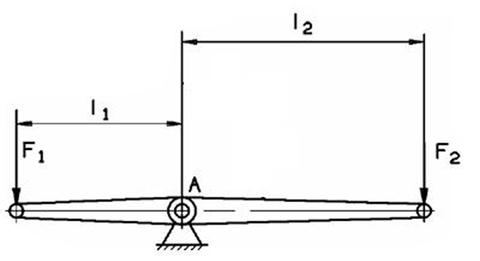
\includegraphics[width=0.48\linewidth,keepaspectratio]{graphics/v11_zweiseitiger_hebel.png}\hfill
  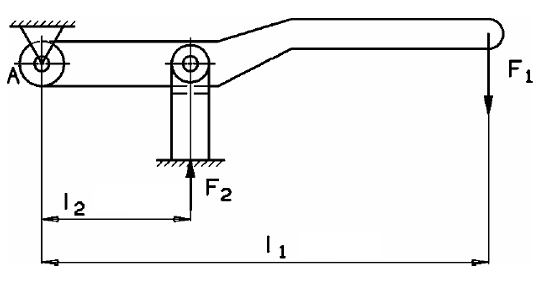
\includegraphics[width=0.48\linewidth,keepaspectratio]{graphics/v11_einseitiger_hebel.png}\par}
  \formulasep
  \ZSFkeyword*{Hebelgesetz}:~$\displaystyle F_2 = \frac{l_1}{l_2} \cdot F_1 = k \cdot F_1$
  \formulanote{Reihenschaltung: $\displaystyle F_3 = \frac{l_1}{l_2}\cdot \frac{l_3}{l_4} \cdot F_1 = k_1 \cdot k_2 \cdot F_1$}
\end{defbox}

\begin{defbox}[Kniehebel]
  \noindent
  \begin{minipage}[c]{0.16\linewidth}
    \centering
    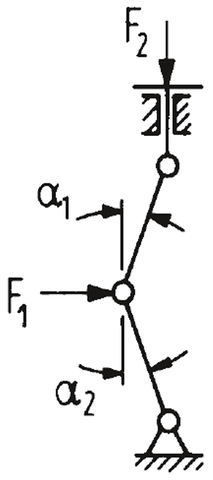
\includegraphics[width=\linewidth,keepaspectratio]{graphics/v11_toggle_lever_force_ratio.png}
  \end{minipage}%
  \hfill
  \begin{minipage}[c]{0.80\linewidth}
    \centering
    $\displaystyle
    \begin{aligned}
      F_2 &= \frac{F_1}{\tan\alpha_1 + \tan\alpha_2} = \frac{F_1}{2\cdot \tan\alpha} \\[4pt]
      K   &= \frac{1}{2\cdot \tan\alpha}
    \end{aligned}
    $
    \par\ZSFgapXS
    {\ZSFfontNote\ZSFmuted{$K$:~Kräfteverhältnis}}
  \end{minipage}
\end{defbox}
\ZSFindex{Kniehebel}

\begin{defbox}[Kniehebel-Spannvorrichtung (Beispiel)]
  \noindent
  \begin{minipage}[c]{0.38\linewidth}
    \centering
    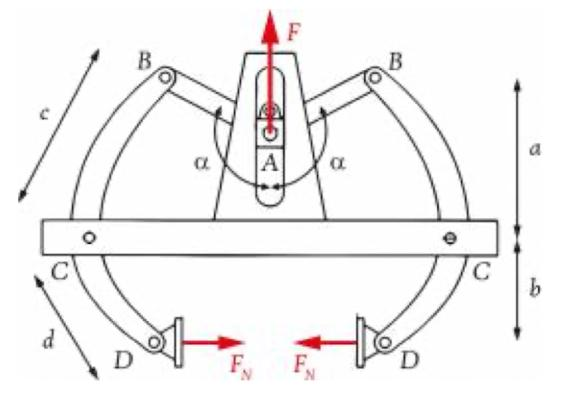
\includegraphics[width=\linewidth,keepaspectratio]{graphics/v11_kniehebel_spannvorrichtung_beispiel.jpeg}
  \end{minipage}%
  \hfill
  \begin{minipage}[c]{0.58\linewidth}
    \centering
    $\displaystyle
    \begin{aligned}
      F_N &= \frac{c \cdot F}{2\cdot \sin(\alpha - 90^\circ)\cdot b} \\[4pt]
          &= \frac{c \cdot F}{2\cdot \cos(180^\circ - \alpha)\cdot b}
    \end{aligned}
    $
  \end{minipage}
\end{defbox}

\SubsubsectionBar{Schiefe Ebene/ Keil}
\ZSFindex{Schiefe Ebene}
\ZSFindex{Keil}

\begin{figbox}
  \begin{minipage}[c]{0.44\linewidth}
    \centering
    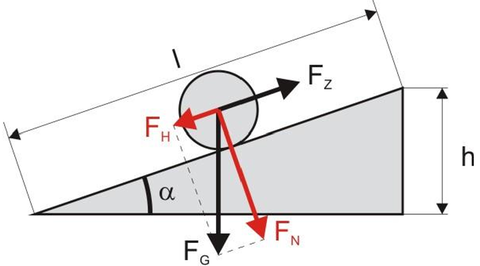
\includegraphics[width=\linewidth,keepaspectratio]{graphics/v11_inclined_plane_forces.png}
    $\displaystyle F_G = \frac{F_z}{\sin\alpha}$ \\[1pt]
    $\displaystyle F_2 = \frac{s_1}{s_2}{\cdot}F_1 = \frac{F_1}{\tan\alpha}$
  \end{minipage}\hfill
  \begin{minipage}[c]{0.52\linewidth}
    \centering
    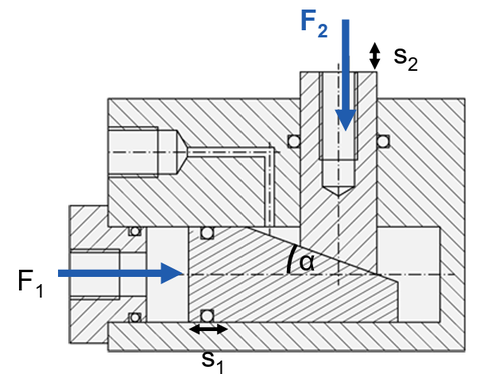
\includegraphics[width=\linewidth,keepaspectratio]{graphics/v11_wedge_force_ratio.png}
  \end{minipage}
\end{figbox}

\SubsubsectionBar{Schraube}

\begin{splitbox}[0.42]
\centering
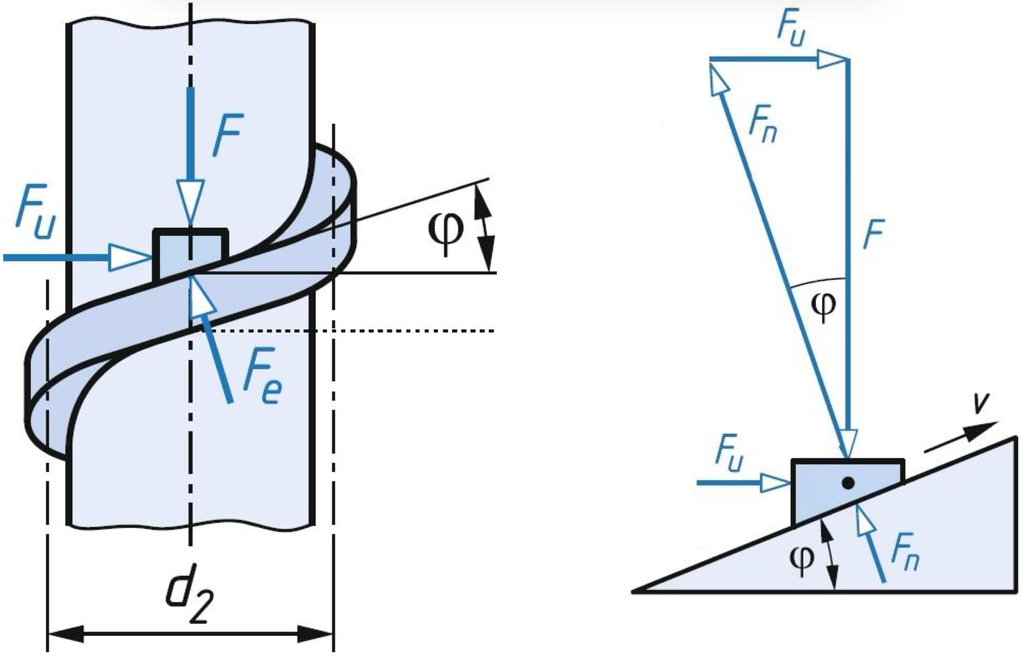
\includegraphics[width=\linewidth,keepaspectratio]{graphics/schraube_als_schiefe_ebene.png}
\tcblower
$\ZSFscrewF = \dfrac{\ZSFscrewFu}{\tan\ZSFscrewPhi}$

\ZSFmuted{Formel \ZSFsource{aus}{sec:schraubenbelastung}}
\end{splitbox}

\SubsubsectionBar{Flaschenzug}
\ZSFindex{Flaschenzug}

\begin{splitbox}[0.54]
\centering
\begin{tikzpicture}[x=1.35pt, y=1.35pt, >=latex, font=\sffamily\fontsize{4.5}{5.5}\selectfont]
  % Example 1: k=1 (Feste Rolle)
  \begin{scope}
    % Decke
    \draw[thick, gray] (1, 40) -- (13, 40);
    \foreach \x in {1,3,...,13} \draw[gray] (\x, 40) -- (\x+1.5, 42.5);

        % Aufhaengung feste Rolle (Ablenkrolle)
    \draw[very thick, ETHRot] (7, 40) -- (7, 30);
    \draw[ETHRot, thick] (5.5, 36.5) -- (8.5, 33.5);
    \draw[ETHRot, thick] (8.5, 36.5) -- (5.5, 33.5);

    % Rolle (weiss gefuellt)
    \draw[thick, fill=white] (7, 30) circle (4);
    \fill (7, 30) circle (1.2);

    % Seil (k=1)
    \draw[very thick, \chaptercolor] (3, 12) -- (3, 30);
    \draw[very thick, \chaptercolor] (3, 30) arc (180:0:4);
    \draw[very thick, \chaptercolor, ->] (11, 30) -- (16, 15) node[right, scale=0.8] {$\ZSFpulleyFZ$};

    % Last
    \draw[thick] (3, 12) -- (3, 7);
    \draw[thick, fill=black!10] (0, 7) rectangle (6, -1) node[pos=0.5, scale=0.8] {$\ZSFpulleyFL$};

    % Annotations
    \node[circle, fill=\chaptercolorlight!80, text=\chaptercolor, font=\tiny\bfseries, inner sep=1pt] at (1, 21) {1};
    \node[circle, fill=\chaptercolorlight!80, text=\chaptercolor, font=\tiny\bfseries, inner sep=1pt] at (15, 20) {1};
    \node[circle, fill=MathHLTertiary!15, text=MathHLTertiary, font=\tiny\bfseries, inner sep=1.2pt] at (3, 9.5) {1};
    \node[below, scale=0.8] at (3, -1) {\textbf{$\ZSFpulleyK = 1$}};
  \end{scope}

  % Example 2: k=2 (Faktorenflaschenzug)
  \begin{scope}
    % Decke
    \draw[thick, gray] (21, 40) -- (33, 40);
    \foreach \x in {21,23,...,33} \draw[gray] (\x, 40) -- (\x+1.5, 42.5);

    % Aufhaengung feste Rolle (Ablenkrolle)
    \draw[very thick, ETHRot] (27, 40) -- (27, 30);
    \draw[ETHRot, thick] (25.5, 36.5) -- (28.5, 33.5);
    \draw[ETHRot, thick] (28.5, 36.5) -- (25.5, 33.5);

    % Rollen
    \draw[thick, fill=white] (27, 30) circle (4);
    \fill (27, 30) circle (1.2);
    \draw[thick, fill=white] (27, 15) circle (4);
    \fill (27, 15) circle (1.2);

    % Seil 1 (k=2)
    \draw[very thick, \chaptercolor] (27, 30) -- (23, 15);
    \draw[very thick, \chaptercolor] (23, 15) arc (180:360:4);
    \draw[very thick, \chaptercolor] (31, 15) -- (31, 30);
    \draw[very thick, \chaptercolor] (31, 30) arc (0:180:4);
    \draw[very thick, \chaptercolor, ->] (23, 30) -- (18, 15) node[left, scale=0.8] {$\ZSFpulleyFZ$};

    % Last
    \draw[thick] (27, 15) -- (27, 7);
    \draw[thick, fill=black!10] (24, 7) rectangle (30, -1) node[pos=0.5, scale=0.8] {$\ZSFpulleyFL$};

    % Annotations
    \node[circle, fill=\chaptercolorlight!80, text=\chaptercolor, font=\tiny\bfseries, inner sep=1pt] at (20, 20) {1};
    \node[circle, fill=\chaptercolorlight!80, text=\chaptercolor, font=\tiny\bfseries, inner sep=1pt] at (24.6, 22) {1};
    \node[circle, fill=\chaptercolorlight!80, text=\chaptercolor, font=\tiny\bfseries, inner sep=1pt] at (33, 22) {1};
    \node[circle, fill=MathHLTertiary!15, text=MathHLTertiary, font=\tiny\bfseries, inner sep=1.2pt] at (27, 11) {2};
    \node[below, scale=0.8] at (27, -1) {\textbf{$\ZSFpulleyK = 2$}};
  \end{scope}

  % Example 3: k=4 (Potenzierter Flaschenzug)
  \begin{scope}
    % Decke
    \draw[thick, gray] (39, 48) -- (65, 48);
    \foreach \x in {39,41,...,65} \draw[gray] (\x, 48) -- (\x+1.5, 50.5);

    % Aufhaengung feste Rolle (Ablenkrolle)
    \draw[very thick, ETHRot] (45, 48) -- (45, 35);
    \draw[ETHRot, thick] (43.5, 43) -- (46.5, 40);
    \draw[ETHRot, thick] (46.5, 43) -- (43.5, 40);

    % Rollen
    \draw[thick, fill=white] (45, 35) circle (4);
    \fill (45, 35) circle (1.2);

    \draw[thick, fill=white] (53, 25) circle (4);
    \fill (53, 25) circle (1.2);

    \draw[thick, fill=white] (57, 10) circle (4);
    \fill (57, 10) circle (1.2);

    % Seil 1 (Teal)
    \draw[very thick, \chaptercolor] (57, 48) -- (57, 25);
    \draw[very thick, \chaptercolor] (57, 25) arc (0:-180:4);
    \draw[very thick, \chaptercolor] (49, 25) -- (49, 35);
    \draw[very thick, \chaptercolor] (49, 35) arc (0:180:4);
    \draw[very thick, \chaptercolor, ->] (41, 35) -- (36, 15) node[left, scale=0.8] {$\ZSFpulleyFZ$};

    % Seil 2 (Orange)
    \draw[very thick, MathHLSecondary] (53, 25) -- (53, 10);
    \draw[very thick, MathHLSecondary] (53, 10) arc (180:360:4);
    \draw[very thick, MathHLSecondary] (61, 10) -- (61, 48);

    % Last
    \draw[thick] (57, 10) -- (57, 2);
    \draw[thick, fill=black!10] (53, 2) rectangle (61, -6) node[pos=0.5, scale=0.8] {$\ZSFpulleyFL$};

    % Annotations
    \node[circle, fill=\chaptercolorlight!80, text=\chaptercolor, font=\tiny\bfseries, inner sep=1pt] at (38, 20) {1};
    \node[circle, fill=\chaptercolorlight!80, text=\chaptercolor, font=\tiny\bfseries, inner sep=1pt] at (47.5, 30) {1};
    \node[circle, fill=\chaptercolorlight!80, text=\chaptercolor, font=\tiny\bfseries, inner sep=1pt] at (58.5, 33) {1};
    \node[circle, fill=MathHLSecondary!15, text=MathHLSecondary, font=\tiny\bfseries, inner sep=1pt] at (51.5, 18) {2};
    \node[circle, fill=MathHLSecondary!15, text=MathHLSecondary, font=\tiny\bfseries, inner sep=1pt] at (62.5, 25) {2};
    \node[circle, fill=MathHLTertiary!15, text=MathHLTertiary, font=\tiny\bfseries, inner sep=1.2pt] at (57, 5) {4};
    \node[below, scale=0.8] at (57, -6) {\textbf{$\ZSFpulleyK = 4$}};
  \end{scope}

  % Warning Box: Ablenkrolle (unter Example 1 & 2)
  \begin{scope}[shift={(0,-52)}]
    % Decke
    \draw[thick, gray] (11, 40) -- (23, 40);
    \foreach \x in {11,13,...,23} \draw[gray] (\x, 40) -- (\x+1.5, 42.5);

    % Feste Rolle Support (Ablenkrolle)
    \draw[very thick, ETHRot] (17, 40) -- (17, 30);
    \node[right, ETHRot, scale=0.7, font=\bfseries] at (18, 35) {Ablenkrolle};

    % Pulley
    \draw[thick, fill=white] (17, 30) circle (4);
    \fill (17, 30) circle (1.2);

    % Rope
    \draw[very thick, \chaptercolor] (13, 20) -- (13, 30);
    \draw[very thick, \chaptercolor] (13, 30) arc (180:0:4);
    \draw[very thick, \chaptercolor, ->] (21, 30) -- (26, 15) node[right, scale=0.8] {$\ZSFpulleyFZ$};

    % Red cross on the support
    \draw[ETHRot, thick] (15.5, 36.5) -- (18.5, 33.5);
    \draw[ETHRot, thick] (18.5, 36.5) -- (15.5, 33.5);

    % Annotations
    \node[circle, fill=\chaptercolorlight!80, text=\chaptercolor, font=\tiny\bfseries, inner sep=1pt] at (11, 25) {1};
    \node[circle, fill=\chaptercolorlight!80, text=\chaptercolor, font=\tiny\bfseries, inner sep=1pt] at (25, 23) {1};
  \end{scope}
\end{tikzpicture}
\tcblower
\ZSFReadableOn
\ZSFkeyword{Kraftzahl-Methode} zur Bestimmung von \mbox{$\ZSFpulleyFZ = \ZSFpulleyFL / \ZSFpulleyK$}:
\begin{enumerate}[leftmargin=1.1em, itemsep=1.5pt, parsep=0pt, topsep=1pt]
  \item \textbf{\color{\chaptercolor}Zugende = 1}: Das Seilende am Kraftangriff $\ZSFpulleyFZ$ erh\"alt die Kraftzahl \textcolor{\chaptercolor}{\textbf{1}}.
  \item \textbf{\color{\chaptercolor}Gleiches Seil}: Ein ununterbrochenes Seil hat \"uberall dieselbe Kraftzahl.
  \item \textbf{\color{MathHLSecondary}Rollen-Summe}: Eine lose Rolle addiert die Werte ihrer tragenden Seile auf ihre Aufh\"angung (z.\,B. \mbox{\textcolor{MathHLSecondary}{\textbf{2}} = \textcolor{\chaptercolor}{\textbf{1}} + \textcolor{\chaptercolor}{\textbf{1}}}).
  \item \textbf{\color{MathHLTertiary}Last-Summe $\ZSFpulleyK$}: Die Summe aller an der Last ziehenden Seilwerte ergibt \textbf{$\ZSFpulleyK$}.
\end{enumerate}
\par\ZSFgapXS
\ZSFdanger{Ablenkrollen} (fest an Decke) \"andern nur die Richtung und tragen nicht zu \textbf{$\ZSFpulleyK$} bei!
\end{splitbox}


\SubsectionBar[sec:rotation-translation]{Rotation zu Translation}

\SubsubsectionBar{Schubkurbel (Slider Crank)}
\ZSFindex{Schubkurbel}
\ZSFindexsee{Slider Crank}{Schubkurbel}

\begin{runintext}
Tangentialkraft $\ZSFmechFt$ der Kurbel (Rotation) führt zu Kraft im Pleuel $\ZSFmechFp$, führt zu Kraft im Stössel $\ZSFmechFs$ (Translation).
\end{runintext}

\begin{defbox}[Zentrische Schubkurbel]
  {\centering
  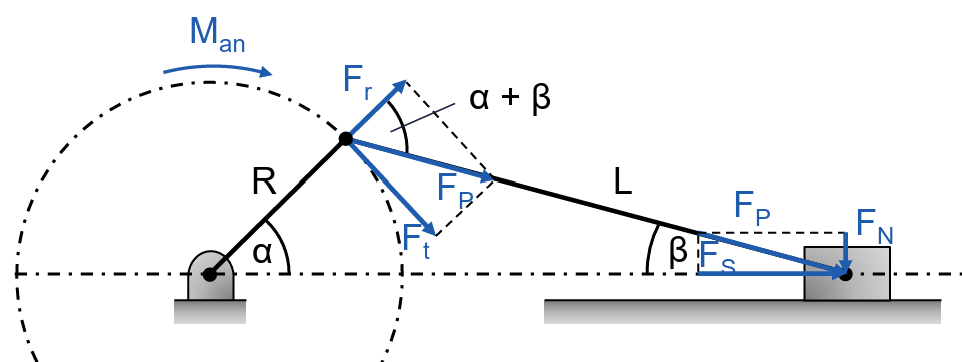
\includegraphics[width=0.85\linewidth,keepaspectratio]{graphics/v11_zentrische_schubkurbel.png}\par}
  \formulasep
  \centering
  $\displaystyle
  \begin{aligned}
    \ZSFmechH &= 2\cdot \ZSFmechR & \ZSFmechT &= \frac{1}{\ZSFmechN} = \frac{60s}{40} \quad (\text{wenn } \ZSFmechN = 40\text{min}^{-1}) \\[4pt]
    \ZSFmechGamma &= \frac{\ZSFmechR}{\ZSFmechL} = \frac{\sin\ZSFmechBeta}{\sin\ZSFmechAlpha} & \ZSFmechFs &= \frac{\cos\ZSFmechBeta \cdot \ZSFmechMan}{\sin(\ZSFmechAlpha+\ZSFmechBeta)\cdot \ZSFmechR}
  \end{aligned}
  $
  \par\ZSFgapXS
  \formulanote{$\ZSFmechH$:~Hub, $\ZSFmechT$:~Taktzeit ($360^\circ$), $\ZSFmechGamma$:~Schubstangenverhältnis ($\frac{R}{L}$, kleiner $\implies$ gleichförmiger), $\ZSFmechR$:~Kurbelradius, $\ZSFmechL$:~Pleuellänge, $\ZSFmechAlpha$/$\ZSFmechBeta$:~Kurbel-/Pleuelwinkel, $\ZSFmechFs$:~Stösselkraft, $\ZSFmechMan$:~Antriebsmoment, $\ZSFmechN$:~Drehzahl}
\end{defbox}

\begin{defbox}[Exzentrische Schubkurbel (Quick-Return)]
  {\centering
  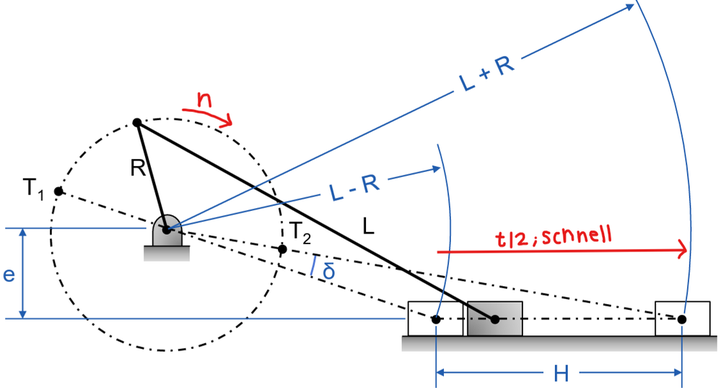
\includegraphics[width=0.70\linewidth,keepaspectratio]{graphics/v11_exzentrische_schubkurbel_quick_return.png}\par}
  \formulasep
  \ZSFkeyword{Zeitenverhältnis} $\ZSFmechQ$:~\par\ZSFgapXS
  \centering
  $\displaystyle \ZSFmechQ = \frac{\ZSFmechTslow}{\ZSFmechTfast} = \frac{180^\circ + \ZSFmechDelta}{180^\circ - \ZSFmechDelta}
  \quad \ZSFmechDelta = 180^\circ \cdot \frac{\ZSFmechQ - 1}{\ZSFmechQ+1}
  \quad \ZSFmechTges = \ZSFmechTslow + \ZSFmechTfast = \frac{1}{\ZSFmechN}$ \\[4pt]
  $\displaystyle \ZSFmechTfast = \frac{180^\circ - \ZSFmechDelta}{360^\circ} \cdot \frac{60}{\ZSFmechN}
  \quad \ZSFmechTslow = \frac{180^\circ + \ZSFmechDelta}{360^\circ} \cdot \frac{60}{\ZSFmechN}$
  \par\ZSFgapS
  \begin{factlist}
    \item Falls Winkel zwischen $T_1$ und $T_2 < 180^\circ \rightarrow$ schnell
    \item Falls Winkel zwischen $T_1$ und $T_2 > 180^\circ \rightarrow$ langsam
    \item $\ZSFmechEcc \uparrow \implies \ZSFmechDelta \uparrow \implies \ZSFmechQ \uparrow$
  \end{factlist}
  \par\ZSFgapXS
  \formulanote{$\ZSFmechQ$:~Zeitenverhältnis, $\ZSFmechTslow$/$\ZSFmechTfast$:~Zeit langsam/schnell, $\ZSFmechDelta$:~Symmetriewinkel, $\ZSFmechEcc$:~Exzentrizität}
\end{defbox}
\ZSFindex{Quick-Return}

\SubsubsectionBar{Kurbelschleife (Quick-Return)}
\ZSFindex{Kurbelschleife}

\begin{splitbox}[0.55]
\centering
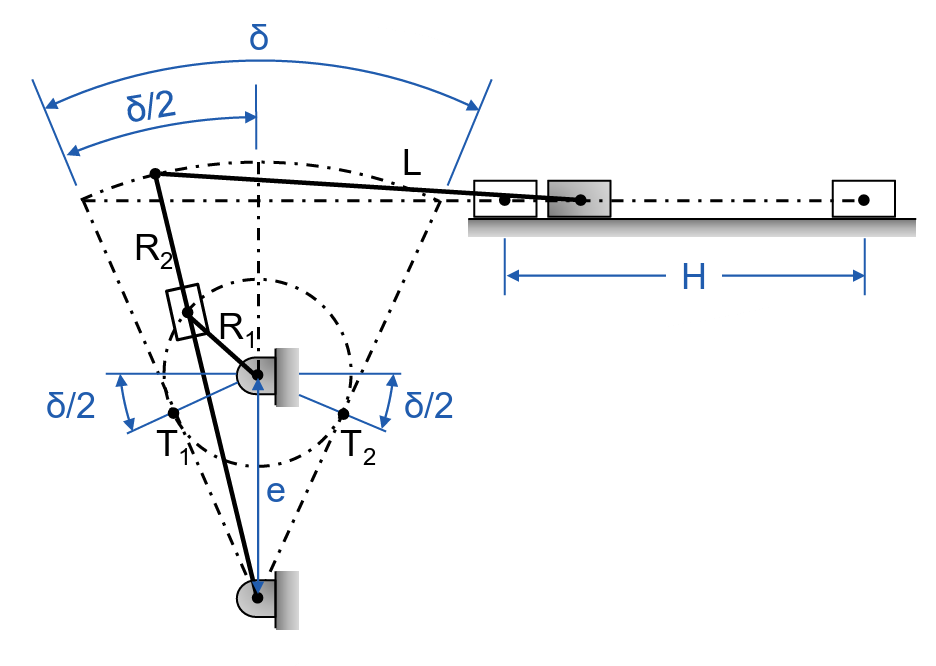
\includegraphics[width=\linewidth,keepaspectratio]{graphics/v11_kurbelschleife_quick_return.png}
\tcblower
$\sin(\dfrac{\ZSFmechDelta}{2})= \dfrac{\ZSFmechROne}{\ZSFmechEcc} = \dfrac{\ZSFmechH}{2\cdot \ZSFmechRTwo}$

$\ZSFmechQ = \dfrac{180° + \ZSFmechDelta}{180° - \ZSFmechDelta}$

$\ZSFmechTslow/\ZSFmechTfast = \dfrac{180° \pm \ZSFmechDelta}{360°} \cdot \dfrac{60}{\ZSFmechN}$
\par\ZSFgapXS
\formulanote{$\ZSFmechROne$:~Antriebsradius, $\ZSFmechRTwo$:~Schwingenlänge, $\ZSFmechEcc$:~Pivot-Abstand}
\end{splitbox}


\SubsubsectionBar{Viergelenkkette (Four Bar Linkage)}
\ZSFindex{Viergelenkkette}
\ZSFindexsee{Four Bar Linkage}{Viergelenkkette}

\begin{splitbox}[0.38]
\ZSFindex[drehfahigkeit]{Drehfähigkeit}
\ZSFkeyword*{Drehfähigkeit}:~"Die Kurbel ist voll drehfähig, wenn die Summe des kleinsten und grössten Stabes kleiner als die Summe der mittleren Stäbe ist."
\par\ZSFgapXS
{\ZSFfontNote \textbf{Grenzgetriebe} (durchschlagend): Summe zweier Stäbe = Summe der anderen}
\par\ZSFgapXS
{\sffamily\fontsize{5.8bp}{6.3bp}\selectfont
\begin{enumerate}[leftmargin=1.0em, itemsep=0.5pt, parsep=0pt, topsep=1pt]
  \item Kurbelschwinge
  \item Kurbelschwinge
  \item durchsch. Kurbelschwinge
  \item durchsch. Kurbelschwinge
  \item Kurbelschwinge
  \item Parallelkurbelgetriebe
  \item durchsch. Kurbelschwinge
\end{enumerate}
}
\tcblower
\centering
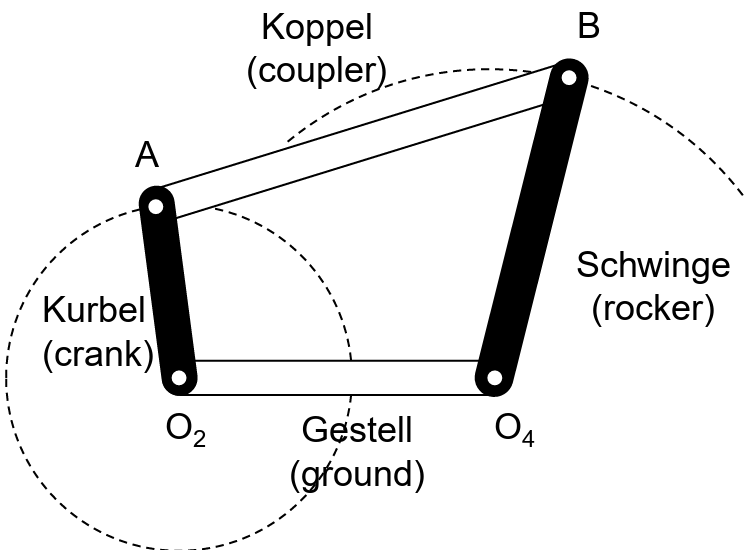
\includegraphics[width=0.86\linewidth,keepaspectratio]{graphics/v11_viergelenkkette_four_bar_linkage.png}
\end{splitbox}






\ZSFfig[1.0]{graphics/v11_four_bar_rotatability_cases.png}{}{}

\SubsubsectionBar{Koppelgetriebe}
\ZSFindex{Koppelgetriebe}

% Spalten-Packung (6-Seiten-Ziel): Bilderstapel in zwei figboxen geteilt,
% damit die Teile an Spaltenenden umbruchfähig sind. Bildgrössen unverändert.
\begin{figbox}
\centering
% kein \quad: 0.35+0.62+quad > Zeilenbreite -> Bilder wuerden untereinander rutschen
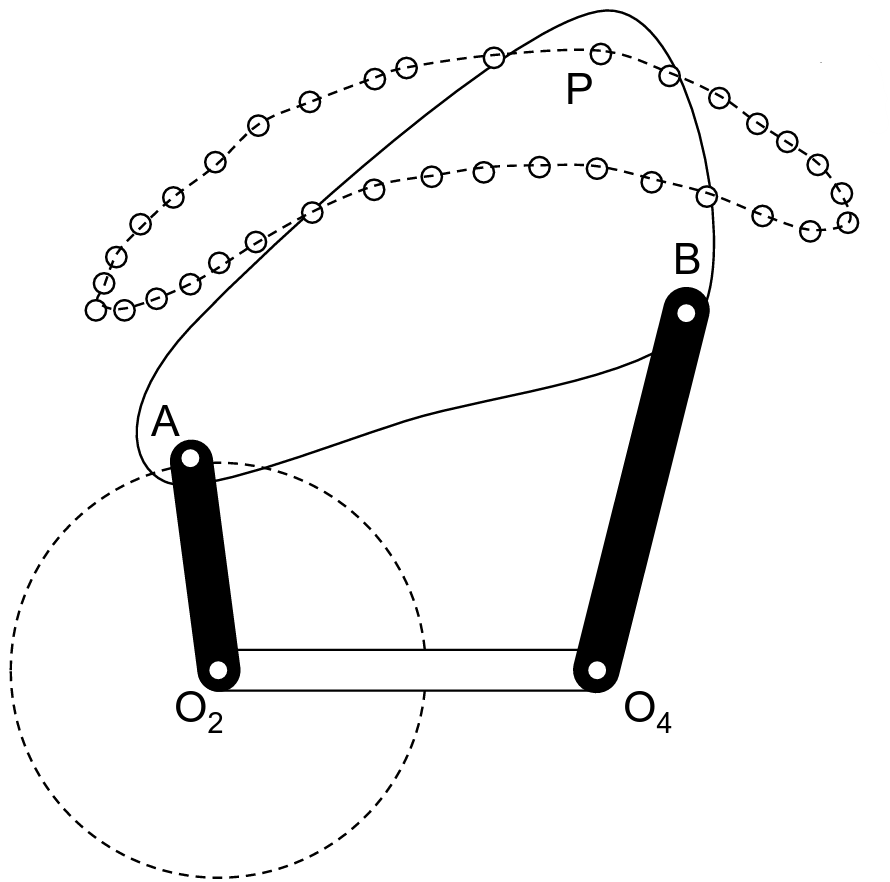
\includegraphics[width=0.35\linewidth,keepaspectratio]{graphics/v11_koppelkurve.png}
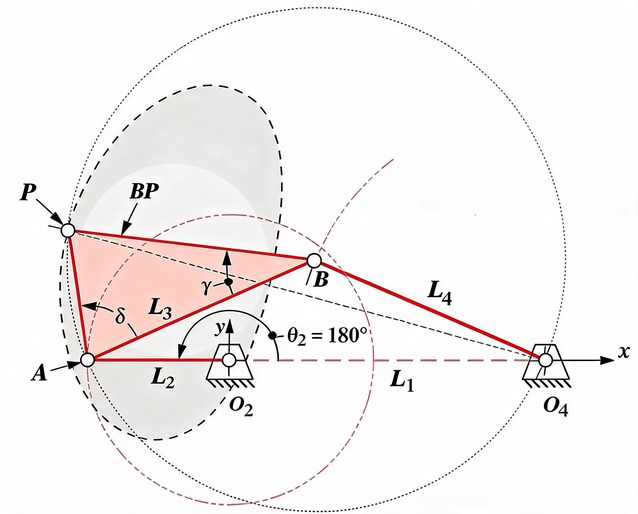
\includegraphics[width=0.62\linewidth,keepaspectratio]{graphics/v11_coupler_mechanism_lengths_angles.jpg}
\end{figbox}

% !TEX root = ../main.tex
% SECTION 10: GESTALTUNG UND FERTIGUNG
% Inhalt: Liv Erne, Silvio Seiz — Form: ZSF-Template-Rework
% ============================================================

\StartChapter[ch:fertigung]{Gestaltung und Fertigung}

\begin{factlist}
\ZSFFact{Idealgestalt}{$\leftarrow$ Lösungsprinzip}
\ZSFFact{Realgestalt}{$\leftarrow$ Betrieb, Werkstoffe, Wirtschaft, Umwelt und Herstellung}
\end{factlist}

\SubsectionBar[sec:fertigungsverfahren]{Fertigungsverfahren}
\ZSFindex{Fertigungsverfahren}
\ZSFindex{Urformen}
\ZSFindex{Umformen}
\ZSFindex{Trennen}
\ZSFindex[fugen]{Fügen}
\ZSFindex{Beschichten}

\SubsubsectionBar*{1. Urformen}
\ZSFverfahrenBefore
{\centering
\begin{tikzpicture}[font=\ZSFfontTableDense]
\matrix[ZSFverfahrenmatrix, name=mat] {
Giessen & Zahnbürsten, Motorkolben \\
Sintern & Bremsbeläge, Zahnräder \\
Additive Manuf. & 1.~Bauteilentwicklung am CAD-System\newline 2.~Slice-Vorgang\newline 3.~Bauteilerstellung an der SLM-Maschine\newline 4.~Bauteilnachbearbeitung \\
};
\ZSFverfahrenconnectors{3}
\end{tikzpicture}\par}

\SubsubsectionBar*{2. Umformen}
\ZSFverfahrenBefore
{\centering
\begin{tikzpicture}[font=\ZSFfontTableDense]
\matrix[ZSFverfahrenmatrix, name=mat] {
Walzen & Bleche, Schienen \\
Schmieden & Hufeisen, Werkzeug \\
Tiefziehen & Alu-Dosen, Invisalign \\
};
\ZSFverfahrenconnectors{3}
\end{tikzpicture}\par}

\SubsubsectionBar*{3. Trennen}
\ZSFverfahrenBefore
{\centering
\begin{tikzpicture}[font=\ZSFfontTableDense]
\matrix[ZSFverfahrenmatrix, name=mat] {
Drehen & Antriebsachsen \\
Fräsen & MacBook-Casing \\
Schleifen & Präzisionslager, Linsen \\
Schneiden/Stanzen & Fahrrad-Bremsscheiben \\
};
\ZSFverfahrenconnectors{4}
\end{tikzpicture}\par}

\SubsubsectionBar*{4. Fügen}
\ZSFverfahrenBefore
{\centering
\begin{tikzpicture}[font=\ZSFfontTableDense]
\matrix[ZSFverfahrenmatrix, name=mat] {
Schweissen & Stahlrahmen, Brücken \\
Löten & Leiterplatten, Kupferrohr \\
Kleben & Windschutzscheiben, CFK-Bauteile \\
};
\ZSFverfahrenconnectors{3}
\end{tikzpicture}\par}

\SubsubsectionBar*{5. Beschichten}
\ZSFverfahrenBefore
{\centering
\begin{tikzpicture}[font=\ZSFfontTableDense]
\matrix[ZSFverfahrenmatrix, name=mat] {
Lackieren & Karosserie, Möbel \\
Galvanisieren & Chromfelgen, Schmuck \\
PVD / CVD & Werkzeuge, Solarzellen \\
};
\ZSFverfahrenconnectors{3}
\end{tikzpicture}\par}

\SubsubsectionBar*{6. Stoffeigensch. ändern}
\ZSFverfahrenBefore
{\centering
\begin{tikzpicture}[font=\ZSFfontTableDense]
\matrix[ZSFverfahrenmatrix, name=mat] {
Härten & Getriebewellen, Werkzeugstahl \\
Glühen & Federstahl, Kaltumformteile \\
Nitrieren & Kurbelwellen, Zahnräder \\
};
\ZSFverfahrenconnectors{3}
\end{tikzpicture}\par}

% !TEX root = ../main.tex
% SECTION 11: ELEKTROMOTOREN
% Inhalt: Liv Erne, Silvio Seiz — Form: ZSF-Template-Rework
% ============================================================

\StartChapter[ch:elektromotoren]{Elektromotoren}
\ZSFindex{Elektromotor}

\SubsectionBar[sec:dc-motoren]{DC-Motoren (Permanentmagneterregte Gleichstrommotoren)}
\ZSFindex{DC-Motor}
\ZSFindexsee{Gleichstrommotor}{DC-Motor}

\ZSFfig[0.9]{graphics/v13_dc_motor_aufbau.png}{}{}

\begin{runintext}
\ZSFReadableOn
\ZSFkeyword{Stator}:~ortsfestes Magnetfeld. \ZSFkeyword{Rotor}:~Spulen erzeugen Drehbewegung durch Anziehung/Abstossung. \ZSFkeyword{Kommutator}:~mitdrehende Ringsegmente + ortsfeste Kohlebürsten wechseln Stromrichtung in Spulen bei Drehung.
\end{runintext}

\begin{figbox}[Vor und nach Stromrichtungswechsel]
\centering
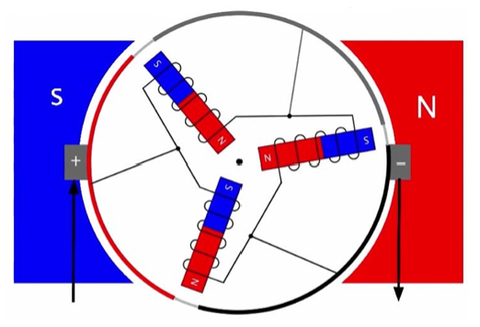
\includegraphics[width=0.27\linewidth,keepaspectratio]{graphics/v13_dc_motor_vor_stromrichtungswechsel.png}\quad
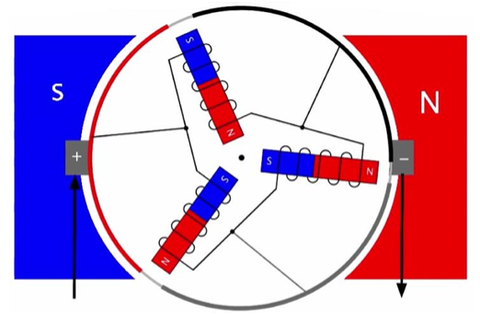
\includegraphics[width=0.27\linewidth,keepaspectratio]{graphics/v13_dc_motor_nach_stromrichtungswechsel.png}
\end{figbox}

\begin{formulabox}[Kennwerte \& Konstanten]
$1\cdot \dfrac{A}{mNm} = 60'000 \cdot \dfrac{min^{-1}}{V}$

$\ZSFmotorKn = \dfrac{1}{2\pi \ZSFmotorKm}\, [\dfrac{s^{-1}}{V}] \rightarrow \cdot 60 = [\dfrac{min^{-1}}{V}]$

$\ZSFmotorKm = \dfrac{\ZSFmotorM}{\ZSFmotorI} \qquad \ZSFmotorIZero = \dfrac{\ZSFmotorMR}{\ZSFmotorKm}$
\formulanote{$\ZSFmotorKn$:~Drehzahlkonst., $\ZSFmotorKm$:~Drehmomentkonst.}
\end{formulabox}

\phantomsection\label{formula:motor-drehzahl}
\begin{formulabox}[Drehzahl]
$\ZSFmotorN = \ZSFmotorKn \cdot \ZSFmotorU \ [min^{-1}] \qquad \ZSFmotorNZero = \ZSFmotorKn \cdot (\ZSFmotorUN - \ZSFmotorIZero \cdot \ZSFmotorR)$

$\ZSFmotorN = \ZSFmotorKn \cdot (\ZSFmotorUN - \ZSFmotorIZero \cdot \ZSFmotorR) - \dfrac{\ZSFmotorKn}{\ZSFmotorKm}\cdot \ZSFmotorR \cdot \ZSFmotorM = \ZSFmotorNZero - \dfrac{\ZSFmotorNZero \cdot \ZSFmotorM}{\ZSFmotorMH}$
\formulanote{$\ZSFmotorUN$:~Nennspannung \ $\cdot$ \ $\ZSFmotorIZero$:~Leerlaufstrom \ $\cdot$ \ $\ZSFmotorNZero$:~Leerlaufdrehzahl \ $\cdot$ \ $\ZSFmotorR$:~Wicklungswiderstand}
\end{formulabox}

\begin{splitbox}[0.39]
  \begin{figbox}[Motorkennlinien]
    \centering
    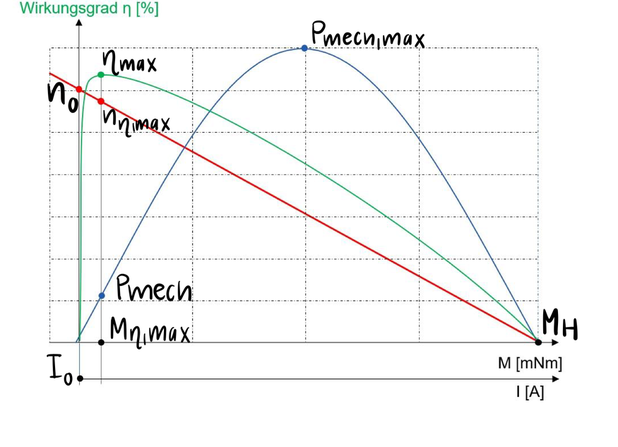
\includegraphics[width=\linewidth,keepaspectratio]{graphics/dc_motor_motorkennlinien_drehmoment_wirkungsgrad_leistung.png}
  \end{figbox}
\tcblower
  \phantomsection\label{formula:motor-drehmoment}
  \begin{formulabox}[Drehmoment]
    \centering
    $\displaystyle \ZSFmotorM = \ZSFmotorKm \cdot \ZSFmotorI \qquad \ZSFmotorMR = \ZSFmotorIZero\cdot \ZSFmotorKm$
    \par\vskip\ZSFspaceXS
    $\displaystyle \ZSFmotorMH = \dfrac{\ZSFmotorNZero \ZSFmotorKm}{\ZSFmotorKn \ZSFmotorR} = (\ZSFmotorUN - \ZSFmotorIZero \ZSFmotorR)\cdot \dfrac{\ZSFmotorKm}{\ZSFmotorR}$
    \par\vskip\ZSFspaceXS
    $\displaystyle \ZSFmotorMMechMax = \dfrac{\ZSFmotorMH - \ZSFmotorMR}{2}$
    \par\vskip\ZSFspaceXS
    $\displaystyle \ZSFmotorMEtaMax = \sqrt{\ZSFmotorMH \cdot \ZSFmotorMR}$
    \formulanote{$\ZSFmotorMH$:~Anhaltemoment, $\ZSFmotorMR$:~Reibmoment}
  \end{formulabox}
\end{splitbox}

\begin{formulabox}[Leistung \& Wirkungsgrad]
\formulasources{$\ZSFmotorN$:~\ZSFsource{aus}{formula:motor-drehzahl}, $\ZSFmotorM$:~\ZSFsource{aus}{formula:motor-drehmoment} \ $\cdot$ \ $\ZSFmotorNZero$:~nur Leerlauf}
$\ZSFmotorPEl = \ZSFmotorU \cdot \ZSFmotorI = \ZSFmotorR \cdot \ZSFmotorI^2 + \ZSFmotorM\cdot 2\pi \ZSFmotorN \qquad \ZSFmotorPMech = 2\pi \ZSFmotorN \ZSFmotorM$

$\ZSFmotorPMechMax = \dfrac{\ZSFmotorR}{4}\cdot (\dfrac{\ZSFmotorUN}{\ZSFmotorR} - \ZSFmotorIZero)^2$

$\ZSFmotorEta = \dfrac{\ZSFmotorPMech}{\ZSFmotorPEl} = \dfrac{-\ZSFmotorR\cdot \ZSFmotorI^2 + (\ZSFmotorU+\ZSFmotorR\cdot \ZSFmotorIZero)\cdot \ZSFmotorI - \ZSFmotorU\cdot \ZSFmotorIZero}{\ZSFmotorU\cdot \ZSFmotorI}$

$\ZSFmotorEtaMax = (1-\sqrt{\dfrac{\ZSFmotorIZero \cdot \ZSFmotorR}{\ZSFmotorUN}})^2$
\end{formulabox}


\ZSFindex{Motorkennlinie}
\ZSFindex{Drehzahlkonstante}
\ZSFindex{Drehmomentkonstante}
\ZSFindex{Anhaltemoment}

\SubsectionBar[sec:servos]{Servos (Geregelte Antriebssysteme)}
\ZSFindex{Servo}

\begin{splitbox}[0.46]
\centering
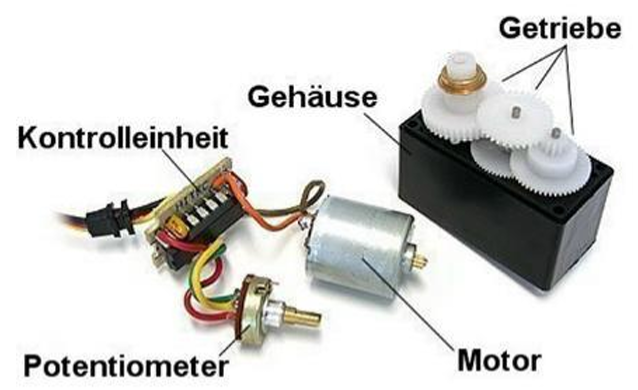
\includegraphics[width=\linewidth,keepaspectratio]{graphics/v13_servo_aufbau_motor_getriebe_potentiometer.png}
\tcblower
\ZSFReadableOn
Ist-Position wird gemessen und mit Soll-Position verglichen. Bei Differenz wird der Motor aktiviert, bis Soll erreicht. Der \ZSFkeyword{Potentiometer} ändert seinen Widerstand je nach Drehwinkel $\ZSFmotorPhi$. Drehbereich: $270^\circ$.
\end{splitbox}

\ZSFfig[0.9]{graphics/v13_servo_blockdiagramm_funktion.png}{}{}

\SubsectionBar[sec:stepper]{Stepper (Hybridschrittmotoren)}
\ZSFindex{Stepper}
\ZSFindexsee{Schrittmotor}{Stepper}

\begin{defbox}[Aufbau]
\ZSFReadableOn
Rotor aus axial magnetisierten \ZSFkeyword{Permanentmagneten} mit gezahnten Polscheiben. Stator aus Kupferspulen mit innenverzahnten Ringsegmenten. Gleiche Teilung, aber Segmente verschoben — nur zwei gegenüberliegende Segmente gleich ausgerichtet.

\formulasep
\noindent
\begin{minipage}[c]{0.48\linewidth}
\centering
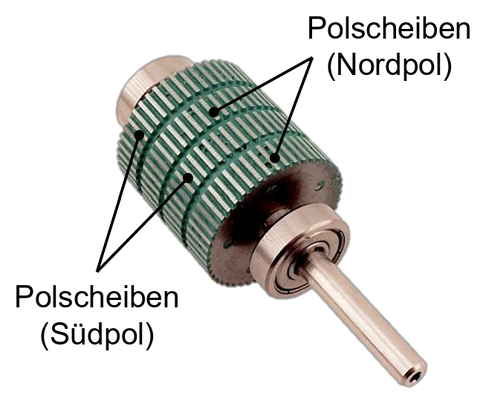
\includegraphics[width=0.75\linewidth,keepaspectratio]{graphics/v13_schrittmotor_aufbau_rotor_polscheiben.png}
\end{minipage}\hfill
\begin{minipage}[c]{0.48\linewidth}
\centering
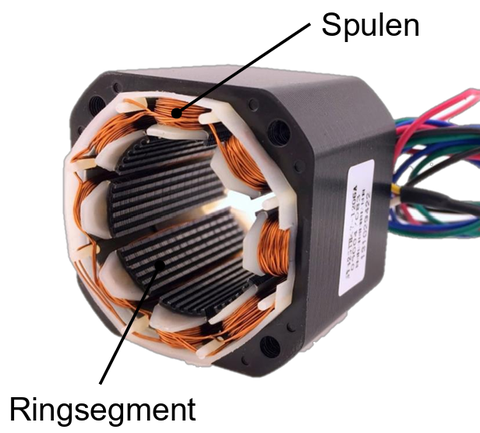
\includegraphics[width=0.75\linewidth,keepaspectratio]{graphics/v13_schrittmotor_aufbau_stator_spulen.png}
\end{minipage}
\end{defbox}

\begin{defbox}[Funktionsweise \& Betriebsarten]
\ZSFReadableOn
\ZSFkeyword*{Funktionsweise}:~Rotation durch schrittweises Spulen-Aktivieren. Gegenüberliegende Spulen zeitgleich \& gleichgerichtet. Versatz um $\tau/2$ $\rightarrow$ max. Anziehung/Abstossung.
\par\formulasep
\noindent
\begin{minipage}[c]{0.48\linewidth}
\centering
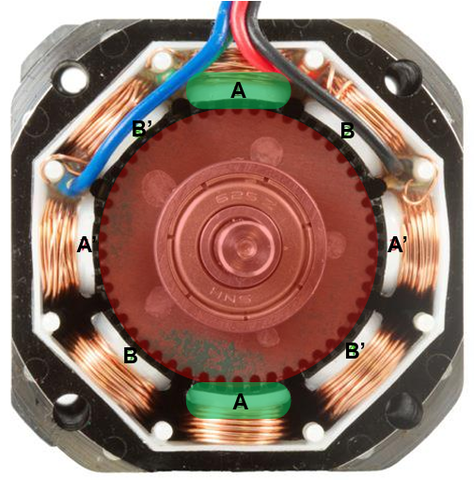
\includegraphics[width=0.72\linewidth,keepaspectratio]{graphics/v13_schrittmotor_unipolarer_betrieb.png}
\end{minipage}\hfill
\begin{minipage}[c]{0.48\linewidth}
\centering
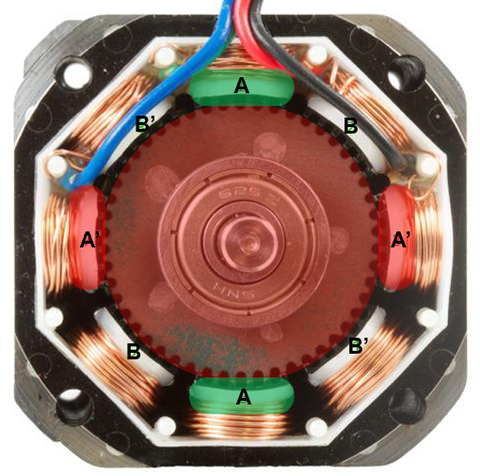
\includegraphics[width=0.72\linewidth,keepaspectratio]{graphics/v13_schrittmotor_bipolarer_betrieb.png}
\end{minipage}
\par\formulasep
\ZSFdanger{Uhrzeigersinn!} bei folgenden Aktivierungsfolgen:
\par\ZSFgapXS
\begin{ZSFtable}[\ZSFfontTableDense]{Z{1.4} Z{1.0} Z{0.9} Z{0.9} Z{0.9} Z{0.9}}
  \ZSFheaderRow
  \ZSFhead{Betrieb} & \ZSFhead{Schritt} & \ZSFhead{A} & \ZSFhead{B} & \ZSFhead{A'} & \ZSFhead{B'} \\
  Unipolar & Halb & grün & grün & aus & aus \\
  Unipolar & Voll & aus & grün & aus & aus \\
  Bipolar & Halb & grün & grün & rot & rot \\
  Bipolar & Voll & aus & grün & aus & rot
\end{ZSFtable}
\par\ZSFgapXS
\ZSFdanger{Halbschritt: Drehmomentschwankung (ungerade Spulenpaare).}\par\ZSFgapXS
\ZSFdanger{Bipolar: höheres Haltemoment, tiefer Wirkungsgrad.}
\end{defbox}
\ZSFindex{unipolarer Betrieb}
\ZSFindex{bipolarer Betrieb}

%
%
%
%
%

\StartChapter[ch:anhang]{Anhang}
\tcbset{breakable}
\renewcommand{\BreakIfNotEnoughSpace}{}
\renewcommand{\BreakIfNotEnoughSpaceChapter}{}
\SubsectionBar{Reib- und Formschluss}
\ZSFindex{Reibschluss}
\ZSFindex{Formschluss}

\ZSFReibschlussFormschlussTabelle

\SubsectionBar[sec:wnv-uebersicht]{WNV-Übersicht (Bauformen erkennen)}
\ZSFindex{Welle-Nabe-Verbindung!Bauformen}

% --- Formschluss: Übersichtsgrid + Vergleichspaar (Mitnehmer) ---
\begin{tablebox}[Formschlüssige WNV\ZSFTitleTag{\ZSFref{sec:wnv-formschluss}}]
  \setlength{\tabcolsep}{2pt}%
  \begin{ZSFtablePlain}{Z{0.78} Y{1.22} Z{0.78} Y{1.22}}
    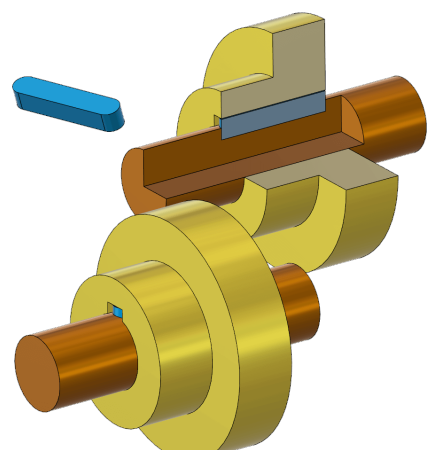
\includegraphics[width=13mm,keepaspectratio]{graphics/wnv_passfeder.png} &
    {\ZSFReadableOn \ZSFkeyword*{Passfeder}\newline 1 Mitnehmer $\Rightarrow$ kleine Momente, günstig} &
    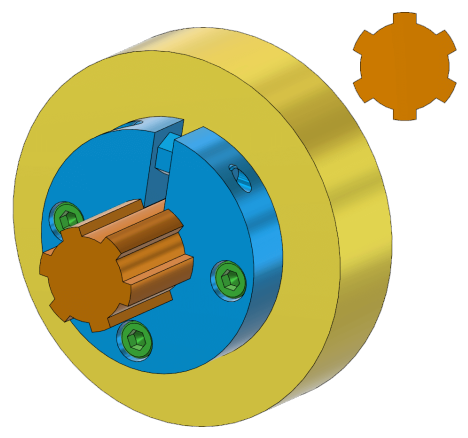
\includegraphics[width=13mm,keepaspectratio]{graphics/wnv_keilwelle.png} &
    {\ZSFReadableOn \ZSFkeyword*{Keilwelle}\newline mehrere Mitnehmer $\Rightarrow$ hohe Momente, teuer} \\
  \end{ZSFtablePlain}
  \ZSFgapXS
  {\centering
  \begin{tikzpicture}
    \node[anchor=south west,inner sep=0] (im) at (0,0)
      {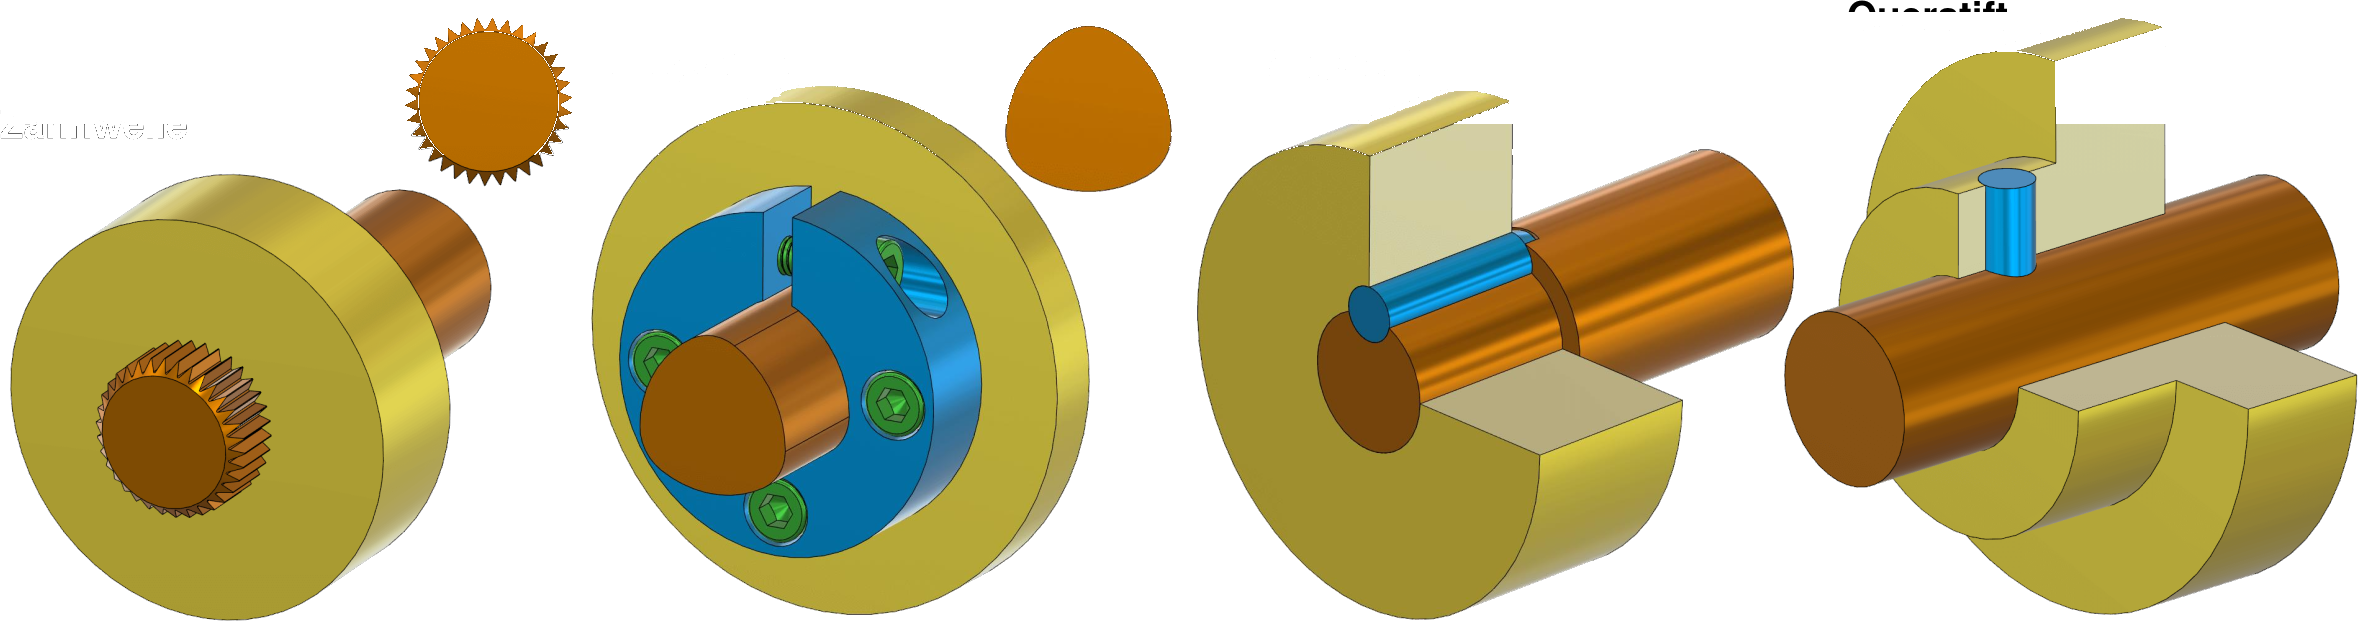
\includegraphics[width=0.72\linewidth,keepaspectratio]{graphics/wnv_uebersicht_formschluss.png}};
    \begin{scope}[x={(im.south east)},y={(im.north west)},
      every node/.style={font=\sffamily\bfseries\fontsize{5}{5.5}\selectfont,
        inner sep=0.5pt, fill=white, fill opacity=0.82, text opacity=1, rounded corners=0.5pt}]
      \node at (0.12,0.87) {Zahnwelle};
      \node at (0.37,0.66) {Polygonprofil};
      \node at (0.62,0.87) {Längsstift};
      \node at (0.88,0.66) {Querstift};
    \end{scope}
  \end{tikzpicture}\par}%
\end{tablebox}
\ZSFindex{Passfeder}
\ZSFindex{Keilwelle}
\ZSFindex{Zahnwelle}
\ZSFindex{Polygonprofil}
\ZSFindex[langsstift]{Längsstift}
\ZSFindex{Querstift}

% --- Reibschluss: Vergleichspaar (Pressverbände) + Übersichtsgrid ---
\begin{tablebox}[Reibschlüssige WNV\ZSFTitleTag{\ZSFref{sec:wnv-reibschluss}}]
  \setlength{\tabcolsep}{2pt}%
  \begin{ZSFtablePlain}{Z{0.78} Y{1.22} Z{0.78} Y{1.22}}
    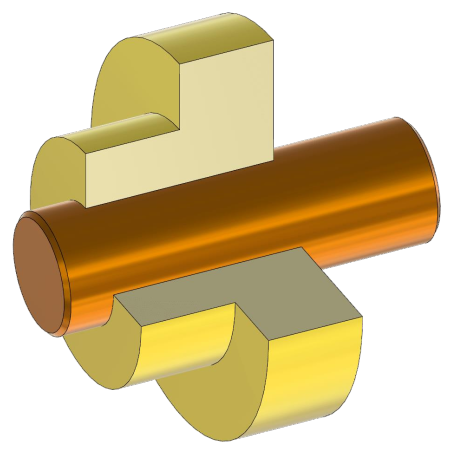
\includegraphics[width=13mm,keepaspectratio]{graphics/wnv_zpv.png} &
    {\ZSFReadableOn \ZSFkeyword*{Zylindr.\ Pressverband} \ZSFref{sec:zpv}\newline Übermass $\Rightarrow$ nicht lösbar, günstig} &
    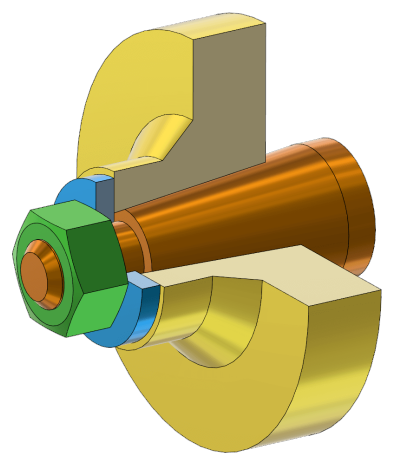
\includegraphics[width=13mm,keepaspectratio]{graphics/wnv_kpv.png} &
    {\ZSFReadableOn \ZSFkeyword*{Kegelpressverband} \ZSFref{sec:kpv}\newline Schraube $\Rightarrow$ lösbar/nachstellbar, teuer} \\
  \end{ZSFtablePlain}
  \ZSFgapXS
  {\centering
  \begin{tikzpicture}
    \node[anchor=south west,inner sep=0] (im) at (0,0)
      {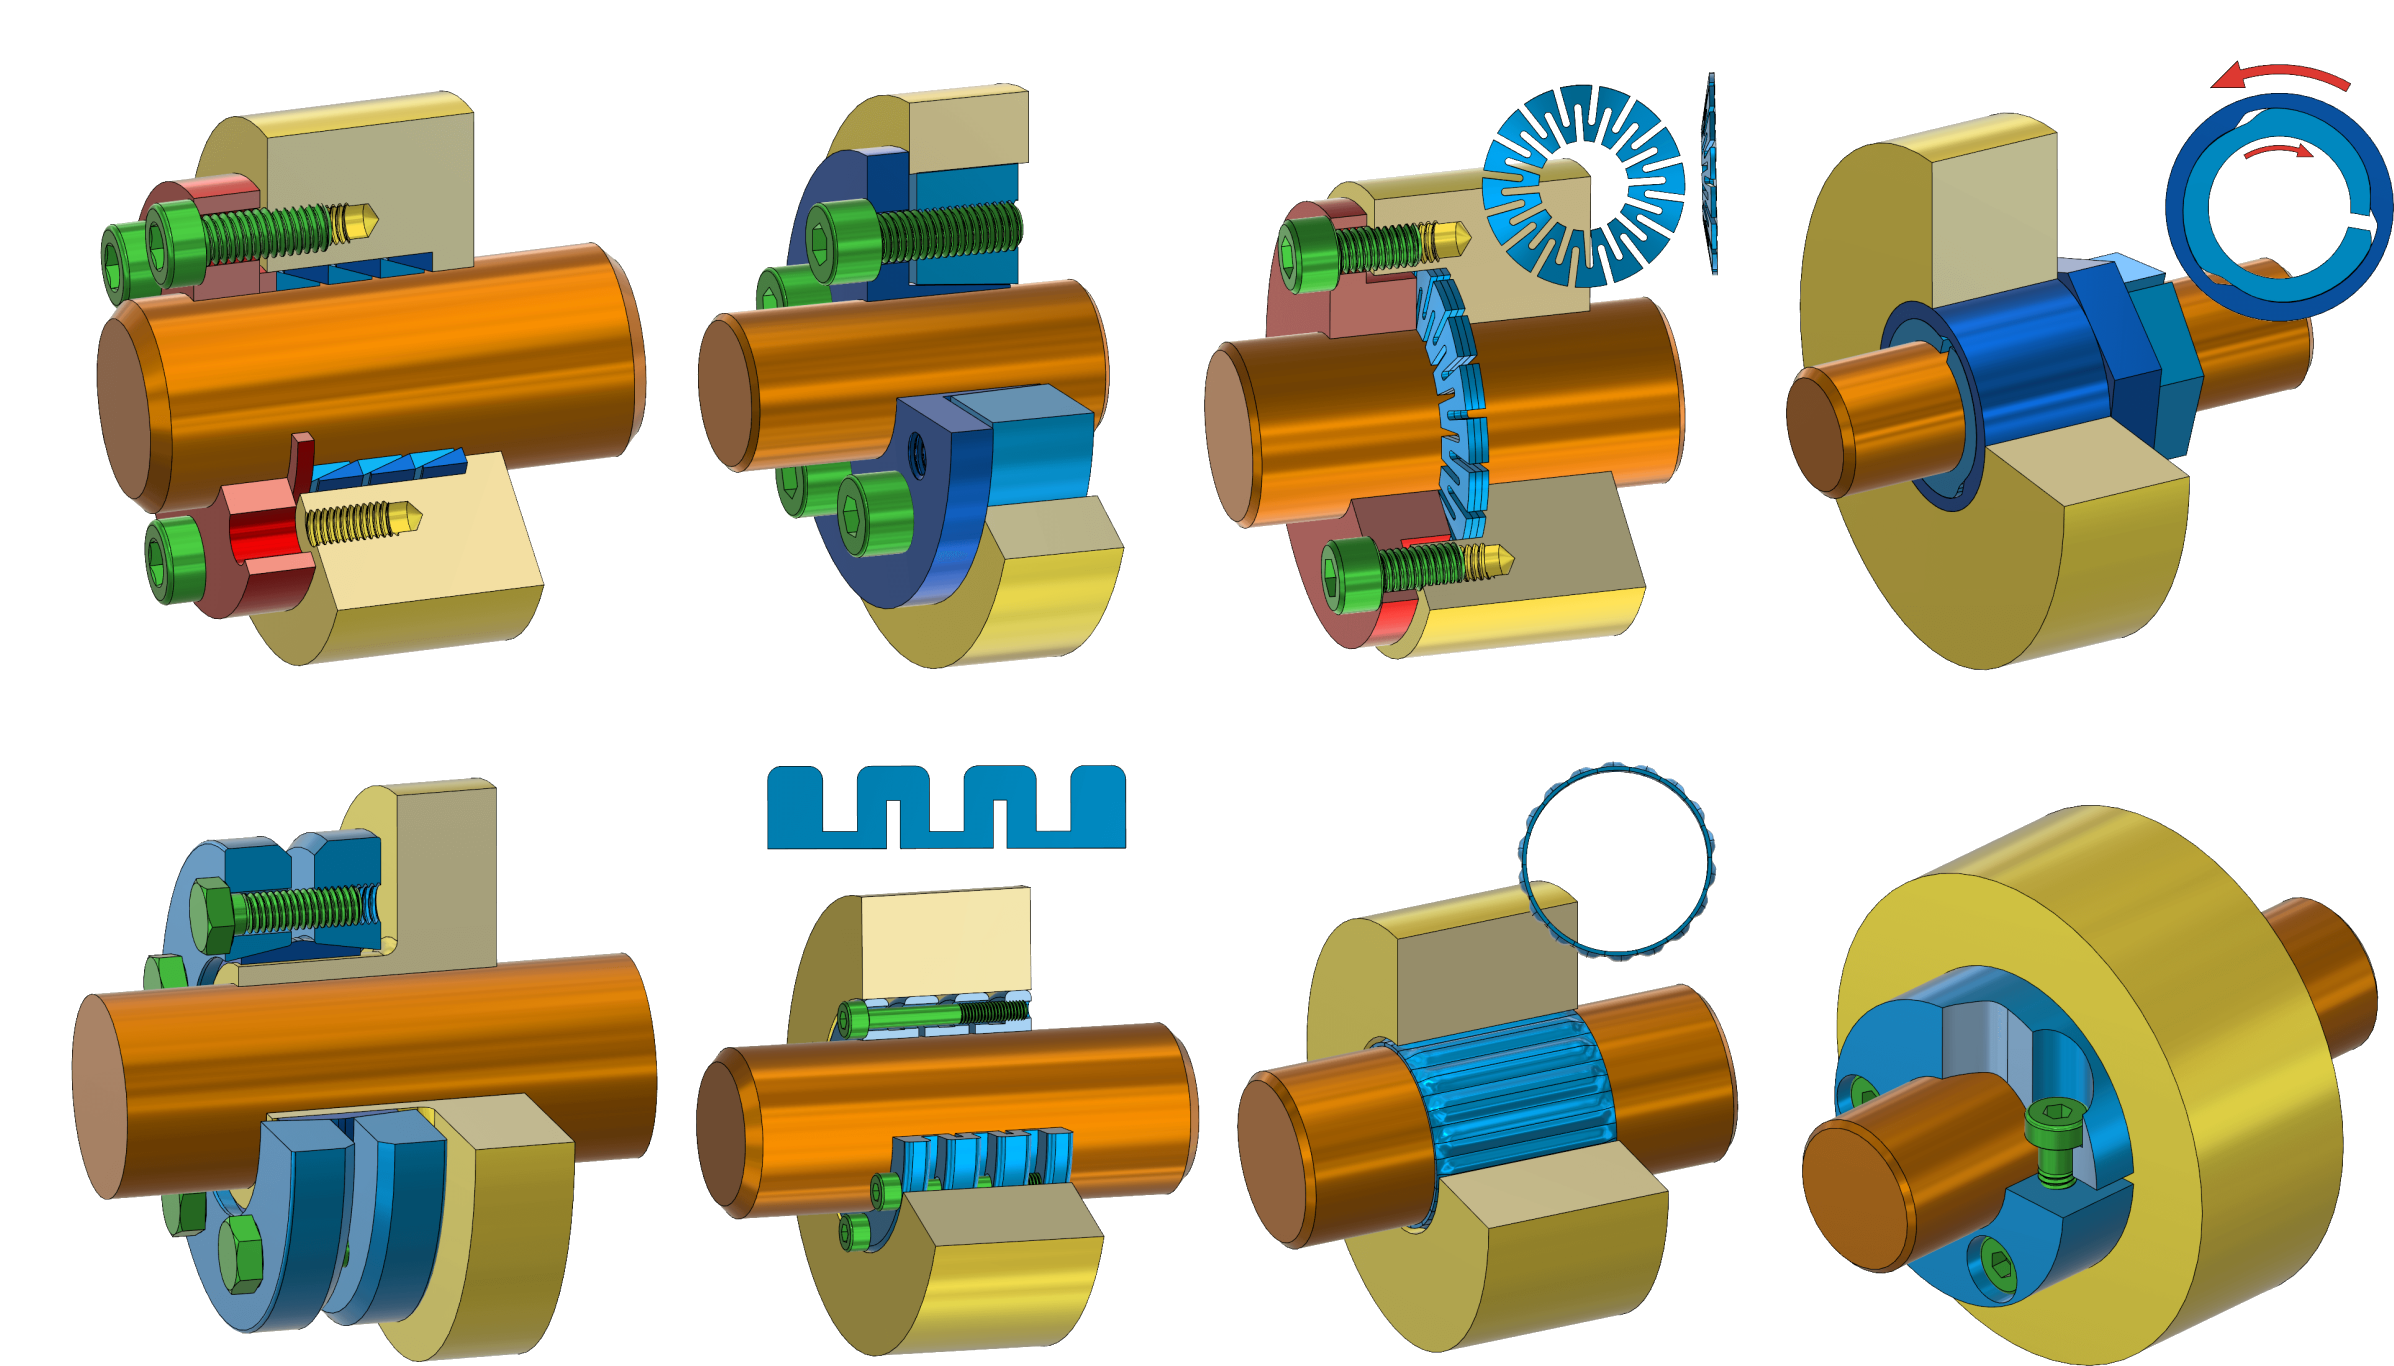
\includegraphics[width=0.72\linewidth,keepaspectratio]{graphics/wnv_uebersicht_reibschluss.png}};
    \begin{scope}[x={(im.south east)},y={(im.north west)},
      every node/.style={font=\sffamily\bfseries\fontsize{5}{5.5}\selectfont,
        inner sep=0.5pt, fill=white, fill opacity=0.82, text opacity=1, rounded corners=0.5pt}]
      \node at (0.13,0.965) {Kegelspannelemente};
      \node at (0.37,0.885) {Kegelspannsatz};
      \node at (0.62,0.965) {Sternscheiben};
      \node at (0.87,0.885) {Kreiskeilverbindung};
      \node at (0.13,0.505) {Schrumpfscheibe};
      \node at (0.37,0.425) {Druckhülse};
      \node at (0.62,0.505) {Toleranzring};
      \node at (0.87,0.425) {Klemmverbindung};
    \end{scope}
  \end{tikzpicture}\par}%
\end{tablebox}
\ZSFindex{Kegelspannelemente}
\ZSFindex{Kegelspannsatz}
\ZSFindex{Sternscheiben}
\ZSFindex{Kreiskeilverbindung}
\ZSFindex{Schrumpfscheibe}
\ZSFindex[druckhulse]{Druckhülse}
\ZSFindex{Toleranzring}
\ZSFindex{Klemmverbindung}

\SubsectionBar[sec:anziehwert]{Anziehwert $\ZSFscrewKA$}
\ZSFindex{Anziehwert}

\ZSFfig[1.0]{graphics/schrauben_anziehwert_ka_tabelle.png}{}{}

\SubsectionBar[sec:nachgiebigkeiten-orte]{Orte der einzelnen Nachgiebigkeiten}

\ZSFfig[0.47]{graphics/schraubenverbindung_nachgiebigkeit_bauteile.png}{}{}

\columnbreak

\SubsectionBar{Lager-Eignungsvergleich}
\ZSFindex{Wälzlagerwahl}
\ZSFindex{Lagereignung}

\ZSFfig[1.0]{graphics/lager_eignung.pdf}{}{}

\SubsectionBar[sec:momverlaeufe]{Dimensionierung \& Momentenverläufe}
\ZSFindex{Momentenverlauf}
\ZSFindex{Welle!Dimensionierung}

\begin{tablebox}[Standard-Lastfälle \& Vorgehen]
  \ZSFReadableOn
  \textbf{Regel}:~Nicht die ganze Welle berechnen -- nur kritische Stellen: kleine $\ZSFstressD$, hohe $\ZSFstressMb$, grosse Kerbwirkungen.\par
  \textbf{Superposition}:~Mehrere Momentenverläufe $\Rightarrow$ $\ZSFstressSigmaV$ an der Stelle max. Auslastung auswerten (kleinstes $\ZSFstressD$, höchstes $\ZSFstressMb$, schärfste Kerbe).
  \par\vskip\ZSFspaceXS
  \setlength{\tabcolsep}{1.0pt}%
  \begin{ZSFtablePlain}{Z{1.0} Z{1.0} Z{1.0}}
    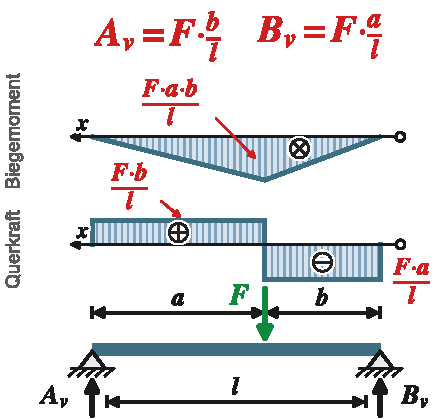
\includegraphics[width=0.98\linewidth]{graphics/momv_1.pdf} &
    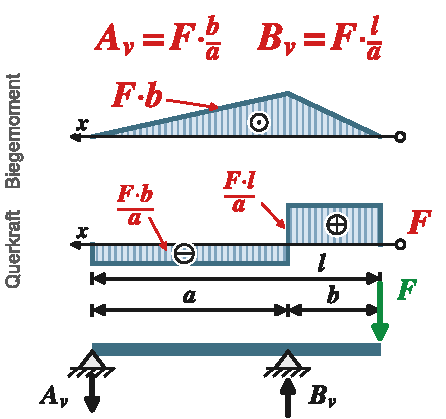
\includegraphics[width=0.98\linewidth]{graphics/momv_2.pdf} &
    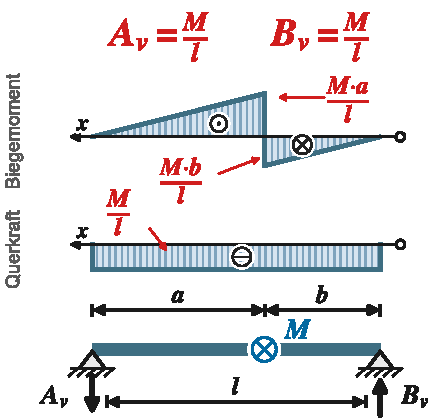
\includegraphics[width=0.98\linewidth]{graphics/momv_3.pdf} \\
    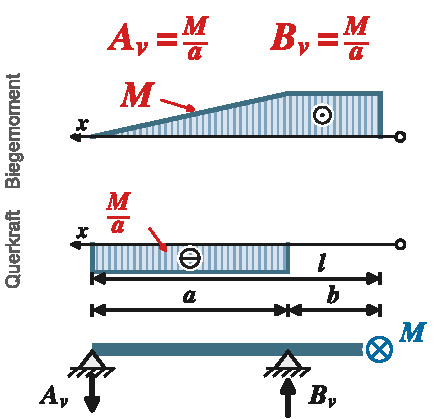
\includegraphics[width=0.98\linewidth]{graphics/momv_4.pdf} &
    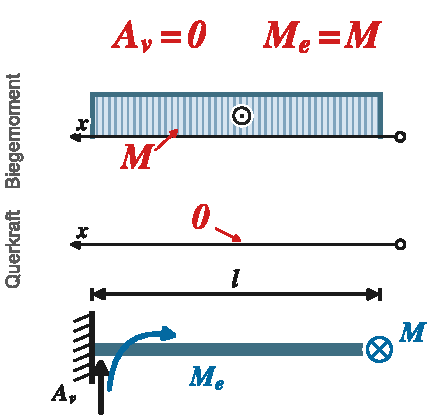
\includegraphics[width=0.98\linewidth]{graphics/momv_5.pdf} &
    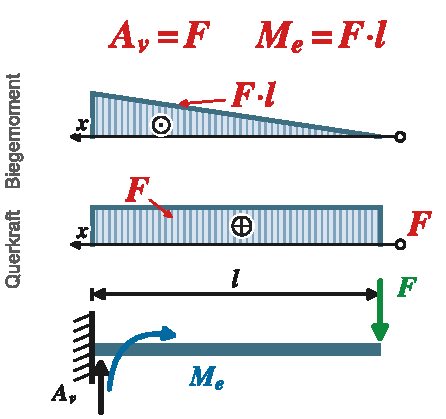
\includegraphics[width=0.98\linewidth]{graphics/momv_6.pdf} \\
    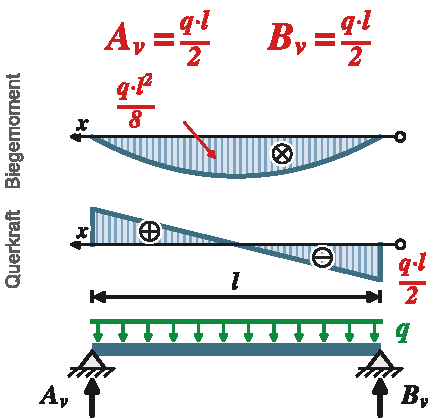
\includegraphics[width=0.98\linewidth]{graphics/momv_7.pdf} &
    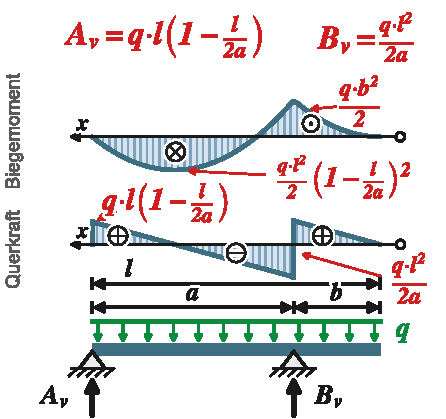
\includegraphics[width=0.98\linewidth]{graphics/momv_8.pdf} &
    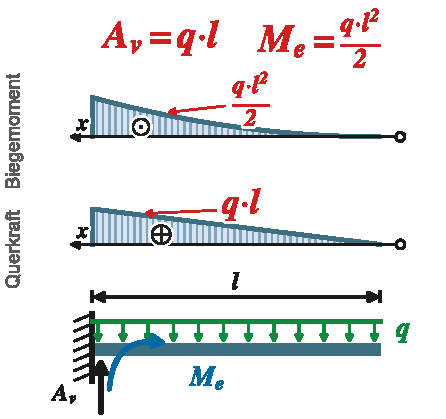
\includegraphics[width=0.98\linewidth]{graphics/momv_9.pdf}
  \end{ZSFtablePlain}
\end{tablebox}

\SubsectionBar[sec:cam-typ]{Kurvenscheiben-Typ (Cam) bestimmen}
\ZSFindex{Kurvenscheibe}
\ZSFindex{Cam}

\begin{defbox}[Kurvenscheiben-Typ (Cam) bestimmen]
  \ZSFReadableOn
  \ZSFkeyword*{Code}:~\textcolor{MechRoleBlue}{\textbf{D}} = \ZSFkeyword{Dwell} (Radius konst. $\Rightarrow$ Stössel ruht), \textcolor{MechRoleGreen}{\textbf{R}} = \ZSFkeyword{Rise} (Radius $\uparrow$), \textcolor{MechRoleRed}{\textbf{F}} = \ZSFkeyword{Fall} (Radius $\downarrow$). $\text{Drehzahl } n = \text{konst.} \Rightarrow$ nur Kontur zählt.
  \par\vskip\ZSFspaceXS
  \setlength{\tabcolsep}{1.0pt}%
  \begin{ZSFtablePlain}{Z{1.0} Z{1.0} Z{1.0} Z{1.0}}
    
\includegraphics[width=0.55\linewidth,keepaspectratio]{graphics/cam_d.pdf} &
    
\includegraphics[width=0.55\linewidth,keepaspectratio]{graphics/cam_rf.pdf} &
    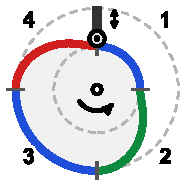
\includegraphics[width=0.55\linewidth,keepaspectratio]{graphics/cam_drdf.pdf} &
    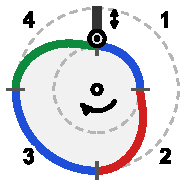
\includegraphics[width=0.55\linewidth,keepaspectratio]{graphics/cam_rdfd.pdf} \\
    {\ZSFfontNote \textcolor{MechRoleBlue}{\textbf{D}}: Kreis konz. $\Rightarrow$ Stössel ruht} &
    {\ZSFfontNote \textcolor{MechRoleGreen}{\textbf{R}}--\textcolor{MechRoleRed}{\textbf{F}}: Exzenter, kein Dwell} &
    {\ZSFfontNote \textcolor{MechRoleBlue}{\textbf{D}}--\textcolor{MechRoleGreen}{\textbf{R}}--\textcolor{MechRoleBlue}{\textbf{D}}--\textcolor{MechRoleRed}{\textbf{F}}: Ziff. = Ber.} &
    {\ZSFfontNote \textcolor{MechRoleGreen}{\textbf{R}}--\textcolor{MechRoleBlue}{\textbf{D}}--\textcolor{MechRoleRed}{\textbf{F}}--\textcolor{MechRoleBlue}{\textbf{D}}: andersrum $\Rightarrow$ inv. + \textcolor{MechRoleGreen}{\textbf{R}} $\leftrightarrow$ \textcolor{MechRoleRed}{\textbf{F}}}
  \end{ZSFtablePlain}
\end{defbox}

\ZSFStartClosingSubsection
\SubsectionBar*{Schlusswort}

\begin{statementbox}
Ich wünsche allen viel Erfolg bei der Prüfung!\par\ZSFgapXS

Den fachlichen Grundstein zu dieser ZSF haben meine Kollegen \ZSFkeyword{Liv Erne} und \ZSFkeyword{Silvio Seiz} gelegt. Ohne die beiden gäbe es diese Zusammenfassung nicht. Ich habe mein eigenes \ZSFkeyword{Hliddal Template} verwendet und hier und da noch ein paar kleine Dinge nach meinem Ermessen angepasst.

\ZSFgapS
\noindent\textbf{Links \& Ressourcen:}
\\
\textbf{Aktuelle Version \& Hliddal Template:}\\
\href{https://garcon-studios.ch/zsf}{garcon-studios.ch/zsf}
\end{statementbox}

% % !TEX root = ../main.tex
% STICHWORTVERZEICHNIS (Opt-in-Modul 66_index)
% Einträge entstehen im Rework über \ZSFkeyword / \ZSFindex / \ZSFindexsee.
% ============================================================

\StartFrontChapter{Stichwortverzeichnis}
\printindex
  % Index ausgetoggelt (Modul 66 bleibt in preamble.tex geladen, da Kapitel \ZSFindex nutzen)

\end{multicols*}
\end{document}
